\PassOptionsToPackage{unicode}{hyperref}

\PassOptionsToPackage{hyphens}{url}
\documentclass[12pt,a4paper,oneside]{report}
\usepackage{xcolor}
\usepackage{amsmath,amssymb}
\setcounter{secnumdepth}{3} % enable section numbering
\usepackage{iftex}
\ifPDFTeX
  \usepackage[T1]{fontenc}
  \usepackage[utf8]{inputenc}
  \usepackage{textcomp} % provide euro and other symbols
\else % if luatex or xetex
  \usepackage{unicode-math} % this also loads fontspec
  \defaultfontfeatures{Scale=MatchLowercase}
  \defaultfontfeatures[\rmfamily]{Ligatures=TeX,Scale=1}
\fi
\usepackage{times}
\usepackage{titlesec}
\usepackage[normalem]{ulem}
\usepackage{setspace}
\singlespacing
\usepackage{graphicx}
\usepackage{subcaption}
% Margins
\usepackage[margin=1in]{geometry}

% Chapter (Main Heading): Bold, 16pt, Center-aligned, ALL CAPS
\titleformat{\chapter}[block]
  {\normalfont\fontsize{16}{20}\bfseries\filcenter\MakeUppercase}
  {\chaptertitlename\ \thechapter:\ }
  {0pt}
  {}
\titlespacing*{\chapter}{0pt}{-20pt}{20pt}

% Section (Sub-heading): Bold, 14pt, Left-aligned
\titleformat{\section}[block]
  {\normalfont\fontsize{14}{18}\bfseries}
  {\thesection\ }
  {0pt}
  {}

% Subsection (Side heading): Bold, 14pt, Left-aligned, Underlined
\titleformat{\subsection}[block]
  {\normalfont\fontsize{14}{18}\bfseries}
  {}
  {0pt}
  {\uline}

\usepackage{lmodern}
\ifPDFTeX\else
  % xetex/luatex font selection
\fi
% Use upquote if available, for straight quotes in verbatim environments
\IfFileExists{upquote.sty}{\usepackage{upquote}}{}
\IfFileExists{microtype.sty}{% use microtype if available
  \usepackage[]{microtype}
  \UseMicrotypeSet[protrusion]{basicmath} % disable protrusion for tt fonts
}{}
\makeatletter
\@ifundefined{KOMAClassName}{% if non-KOMA class
  \IfFileExists{parskip.sty}{%
    \usepackage{parskip}
  }{% else
    \setlength{\parindent}{0pt}
    \setlength{\parskip}{6pt plus 2pt minus 1pt}}
}{% if KOMA class
  \KOMAoptions{parskip=half}}
\makeatother
\usepackage{longtable,booktabs,array}
\newcounter{none} % for unnumbered tables
\usepackage{calc} % for calculating minipage widths
% Correct order of tables after \paragraph or \subparagraph
\usepackage{etoolbox}
\makeatletter
\patchcmd\longtable{\par}{\if@noskipsec\mbox{}\fi\par}{}{}
\makeatother
% Allow footnotes in longtable head/foot
\IfFileExists{footnotehyper.sty}{\usepackage{footnotehyper}}{\usepackage{footnote}}
\makesavenoteenv{longtable}
\usepackage{graphicx}
\makeatletter
\newsavebox\pandoc@box
\newcommand*\pandocbounded[1]{% scales image to fit in text height/width
  \sbox\pandoc@box{#1}%
  \Gscale@div\@tempa{\textheight}{\dimexpr\ht\pandoc@box+\dp\pandoc@box\relax}%
  \Gscale@div\@tempb{\linewidth}{\wd\pandoc@box}%
  \ifdim\@tempb\p@<\@tempa\p@\let\@tempa\@tempb\fi% select the smaller of both
  \ifdim\@tempa\p@<\p@\scalebox{\@tempa}{\usebox\pandoc@box}%
  \else\usebox{\pandoc@box}%
  \fi%
}
% Set default figure placement to htbp
\def\fps@figure{htbp}
\makeatother
\ifLuaTeX
  \usepackage{luacolor}
  \usepackage[soul]{lua-ul}
\else
  \usepackage{soul}
\fi
\setlength{\emergencystretch}{3em} % prevent overfull lines
\providecommand{\tightlist}{%
  \setlength{\itemsep}{0pt}\setlength{\parskip}{0pt}}
\usepackage{bookmark}
\IfFileExists{xurl.sty}{\usepackage{xurl}}{} % add URL line breaks if available
\urlstyle{same}
\hypersetup{
  hidelinks,
  pdfcreator={LaTeX via pandoc}}

\author{}
\date{}
\begin{document}

\begin{titlepage}
\centering
\vspace*{1cm}
{\fontsize{16}{20}\bfseries\MakeUppercase{Pharos University in Alexandria}\par}
\vspace{0.3cm}
{\fontsize{14}{18}\bfseries\MakeUppercase{Faculty of Computer Science and Artificial Intelligence}\par}
\vspace{2cm}
{\fontsize{16}{20}\bfseries\MakeUppercase{APMS: An Integrated Automated Pharmacy Management System with Intellectual Prescription OCR, Robotic Dispensing, and AI-Driven Inventory Analytics}\par}
\vspace{1.5cm}
{\fontsize{14}{18}\bfseries B.Sc. Graduation Thesis\par}
\vspace{1.5cm}
{\large \emph{Submitted by:}\par}
\vspace{0.3cm}
{\large
Ahmed Sherif Hamdy\\
Demiana Said Eshak\\
Mohamed Bakr Mohamed\\
Ghada Mohamed Sedik\\
Youssef Ahmed Ibrahim\\
Nadia Hossny Mohamed\par}
\vspace{1cm}
{\large \emph{Supervised by:}\par}
\vspace{0.3cm}
{\large Dr. Sahar Ghanem\par}
\vfill
{\large June 2026\par}
\end{titlepage}

% Front matter: Roman numeral page numbering
\pagenumbering{roman}

\chapter*{ABSTRACT}
\addcontentsline{toc}{chapter}{Abstract}
Pharmaceutical dispensing and inventory management represent critical
bottlenecks in modern healthcare systems, particularly in community
pharmacies where handwritten prescriptions, manual stock reconciliation,
and high workloads can lead to medical errors and financial
inefficiencies. This thesis presents the \textbf{Automated Pharmacy
Management System (APMS)}, an end-to-end integrated hardware-software
solution that digitizes and automates community pharmacy operations from
prescription entry to mechanical dispensing and inventory optimization.

APMS comprises four core integrated subsystems:

\begin{enumerate}
\def\labelenumi{\arabic{enumi})}
\item
  \textbf{Prescription OCR Core Pipeline}: A vision-language model based
  on GLM-OCR that extracts handwritten drug names from prescription
  images. Spelling mistakes and handwritten irregularities are resolved
  using a novel five-stage sequential fallback search engine that
  queries local and crawl-based external drug databases (FDA, Vezeeta)
  with early-exit criteria and a five-layer safety filter.
\item
  \textbf{AI-Driven Adaptive Robotic Dispensing Hand}: An
  anthropomorphic 3D-printed InMoov robotic hand driven by an ESP32
  microcontroller and five servo motors. It utilizes a continuous
  neural network trained on human demonstrations to interpolate target
  object distances (measured via an HC-SR04 ultrasonic palm sensor) into
  joint angle trajectories, executing distance-adaptive grasps under
  MediaPipe vision guidance.
\item
  \textbf{PharmaSys Dashboard \& Roshetety Patient Mobile App}: A
  full-stack software suite built with Flutter (frontend), Node.js,
  Express, and PostgreSQL (backend), employing WebSockets for real-time
  bidirectional synchronization between mobile patient orders,
  pharmacist approval interfaces, and local serial-port robotic
  dispensing triggers.
\item
  \textbf{AI-Driven Inventory Analytics Engine}: A suite of models
  trained on 60 months of historical pharmacy transaction data. It
  applies a segmented forecasting strategy (LightGBM for fast-moving
  items, Croston's method for slow-moving items, and historical averages
  for intermittent items), computes dynamic expiry-priority scores for
  discount clearance, runs an ECOD-LOF shift anomaly ensemble to flag
  cash reconciliation errors, and trains a Soft Actor-Critic (SAC)
  reinforcement learning agent to optimize monthly replenishment reorder
  decisions, reducing costs by 60\% over classical rule-based inventory policies (Fixed Reorder Point and Min-Max).
\end{enumerate}

Empirical evaluations demonstrate that the robotic arm achieves an
85.7\% grasp success rate and 94.5\% OCR recognition accuracy under
optimal lighting. The sequential fallback search engine reduces API
queries by 72\% compared to parallel voting. Segmented forecasting
improves demand signal capturing by 8.45\% R\textsuperscript{2} over
global models, while the SAC agent converges to an optimal policy in
simulation. This work demonstrates the feasibility of combining low-cost
open-source hardware, state-of-the-art vision-language models, and deep
reinforcement learning to build a secure, on-premise, and affordable
community pharmacy automation system.

\clearpage
\tableofcontents

\clearpage
\addcontentsline{toc}{chapter}{List of Figures}
\listoffigures

\clearpage
\addcontentsline{toc}{chapter}{List of Tables}
\listoftables

\clearpage

% Main matter: Switch to Arabic numeral page numbering
\pagenumbering{arabic}

\chapter{INTRODUCTION}\label{introduction}

\section{Background}\label{background}

The pharmacy industry is currently undergoing a significant digital
transformation. Traditional community pharmacies face numerous
operational challenges, including manual inventory tracking, paper-based
prescription handling, inefficient stock management (leading to either
overstocking or stockouts), and a distinct lack of real-time data-driven
decision-making. In Egypt and the broader Middle East region, the vast
majority of community pharmacies still operate with paper prescriptions,
manual ledger-based inventory systems, and limited technological
integration.

Simultaneously, patient expectations are rapidly evolving. The modern
patient seeks unparalleled levels of convenience---specifically, the
ability to submit prescriptions digitally, track order status in real
time, and communicate securely with pharmacy staff without necessarily
visiting the physical location.

While automation and robotic dispensing have become more accessible,
they have historically been confined to large, high-budget hospital
environments. The lack of integrated software that connects the digital
prescription pipeline from the patient directly to physical on-premise
robotic dispensing hardware remains a significant hurdle for community
pharmacies. Furthermore, medical errors in pharmaceutical dispensing
present a severe threat to patient safety. A primary source of these
errors is the misinterpretation of handwritten medical prescriptions.
Doctors' handwriting is notoriously difficult to read, and many drug
names are visually or phonetically similar (Look-Alike/Sound-Alike or
LASA drugs). When pharmacists misread a prescription, they may dispense
the wrong medication, wrong dosage, or wrong frequency, with potentially
fatal consequences. Automating the extraction and validation of drug
names from handwritten prescriptions via Optical Character Recognition
(OCR)

combined with intelligent search databases represents a crucial safety
layer.

Finally, pharmacy operations are financially constrained. Stock
management is often done heuristically, resulting in expired medicines
(financial write-offs), stockouts of high-demand items (lost revenue and
patient trust), and capital tied up in slow-moving inventory. Optimizing
inventory replenishment through modern machine learning and
decision-support algorithms is critical to making healthcare operations
sustainable.

\section{Problem Statement and Current Situation
Evaluation}\label{problem-statement-and-current-situation-evaluation}

Community pharmacies face several interconnected operational failures
that highlight the inefficiencies of manual systems:

\begin{itemize}
\item
  \textbf{Manual Prescription Handling}: Paper prescriptions are highly
  prone to physical damage, loss, misinterpretation, and administrative
  inefficiency. Pharmacists must manually read handwritten scripts under
  time pressure, leading to critical errors. Traditional OCR systems
  fail on cursive, continuous handwriting, and standard search
  algorithms fail to match misspelled OCR outputs against formal drug
  registries.
\item
  \textbf{Underutilized Automation and Dispensing Latency}: In cases
  where pharmacies possess mechanical dispensing aids, the software
  layer connecting patient orders to robotic hardware is fragmented or
  non-existent. Pharmacists must manually enter commands to trigger
  dispensing, creating a bottleneck.
\item
  \textbf{Inventory Inefficiency}: Stock reordering is performed
  heuristically or based on basic min-max limits. This static approach
  cannot adapt to seasonal demand spikes, leading to overstocking of
  slow items or stockouts of life-saving medications.
\item
  \textbf{Financial Anomaly and Theft Exposure}: Daily shift cash
  reconciliation is performed manually. Due to the high volume of
  micro-transactions, internal theft, manual input errors, and cash
  reconciliation anomalies are difficult for management to detect
  without automated statistical audits.
\item
  \textbf{Patient Communication Gap}: Patients have zero visibility into
  their prescription preparation status once submitted. They are forced
  to wait in long physical queues, reducing overall patient
  satisfaction.
\end{itemize}

\section{User Personas and Stakeholder
Requirements}\label{user-personas-and-stakeholder-requirements}

To ground the system design in real-world constraints, we define three
primary user personas representing different stakeholders:

\begin{enumerate}
\def\labelenumi{\arabic{enumi})}
\item
  \textbf{Dr. Ahmed (Community Pharmacist)}: Dr. Ahmed works in a
  high-traffic community pharmacy. He faces continuous cognitive load,
  handling dozens of prescriptions hourly while answering patient
  inquiries. He requires a system that transcribes handwritten
  prescriptions automatically with high precision, presents the results
  in a clear interface, highlights safety warnings, and allows him to
  trigger robotic dispensing with a single click after verification.
\item
  \textbf{Marian (Chronic Patient)}: Marian is a patient who regularly
  purchases maintenance medication. She values her time and experiences
  frustration when waiting in long pharmacy queues only to find her
  required medication is out of stock. She requires a mobile application
  where she can upload prescription images, view pricing, choose generic
  alternatives, track order progress, and receive notifications when the
  order is ready for pickup or delivery.
\item
  \textbf{Khaled (Pharmacy Business Owner / Inventory Manager)}: Khaled
  manages the pharmacy's financials and supply chain. He is concerned
  about capital locked in dead stock, profit losses due to expired
  drugs, and inventory stockouts. He requires an intelligent dashboard
  that forecasts product-level demand, ranks expiry risk dynamically to
  target clearances, audits cashier shift records for fraud, and
  automates reordering through optimized inventory policies.
\end{enumerate}

\section{Proposed Solution: The Integrated APMS
Framework}\label{proposed-solution-the-integrated-apms-framework}

To address these challenges, we propose the \textbf{Automated Pharmacy
Management System (APMS)}, an end-to-end framework that bridges digital
patient-facing services, intelligent prescription translation, backend
pharmacy operations, and on-premise robotic dispensing. The system
architecture coordinates the following components:

\begin{enumerate}
\def\labelenumi{\arabic{enumi})}
\item
  \textbf{Roshetety Mobile Application}: A mobile interface for patients
  to capture and upload handwritten prescriptions, submit orders, and
  track preparation status in real time.
\item
  \textbf{PharmaSys Staff Dashboard}: An enterprise dashboard for
  pharmacists to verify OCR results, track inventory levels, monitor
  robotic hand status, review financial anomaly reports, and approve
  automated replenishment orders.
\item
  \textbf{Prescription OCR \& Intelligent Search Engine}: A local
  processing pipeline running a vision-language model (GLM-OCR via
  Ollama) and a five-stage sequential fallback search engine that
  resolves spelling errors by querying local tables, fuzzy databases,
  and external web-crawled resources.
\item
  \textbf{Adaptive Grasping Robotic Hand}: A 3D-printed, 5-servo
  mechanical hand that executes distance-adaptive grasping based on
  neural-network interpolation of ultrasonic distance measurements,
  automatically dispensing physical packaging.
\item
  \textbf{AI-Driven Analytics Engine}: A background intelligence layer
  that performs segmented time-series demand forecasting, expiry risk
  scoring, shift reconciliation anomaly detection, and reinforcement
  learning-based reordering.
\end{enumerate}

\section{Research Aims and
Objectives}\label{research-aims-and-objectives}

The specific objectives of this project are:

\begin{itemize}
\item
  To design and print a low-cost, anthropomorphic robotic hand (InMoov
  design) with 16 degrees of freedom (DoF) and 5 active servo actuators.
\item
  To implement a real-time computer vision teleoperation system using
  MediaPipe hand landmark tracking for demonstration recording.
\item
  To train a multi-layer perceptron neural network capable of mapping a
  scalar object distance to a complete continuous servo trajectory for
  adaptive grasping.
\item
  To develop a local OCR pipeline using GLM-OCR and design a sequential
  search fallback engine to match spelling errors against Egyptian and
  global drug databases.
\item
  To construct a robust Node.js backend using TypeScript, PostgreSQL,
  and WebSockets to synchronize order status and serial robotic control.
\item
  To build a responsive staff dashboard and patient app in Flutter.
\item
  To deploy and evaluate time-series forecasting (LightGBM, Croston's)
  and reinforcement learning (Soft Actor-Critic) on a real 60-month
  dataset.
\end{itemize}

These project objectives and their corresponding success metrics are
summarized in Table~\ref{tab:table1}.

\begin{longtable}[]{@{}
  >{\raggedright\arraybackslash}p{(\linewidth - 4\tabcolsep) * \real{0.1823}}
  >{\raggedright\arraybackslash}p{(\linewidth - 4\tabcolsep) * \real{0.2136}}
  >{\raggedright\arraybackslash}p{(\linewidth - 4\tabcolsep) * \real{0.6041}}@{}}
\caption{System Objectives and Success Criteria\label{tab:table1}}\\

\toprule\noalign{}
\begin{minipage}[b]{\linewidth}\raggedright

\textbf{Objective}

\end{minipage} & \begin{minipage}[b]{\linewidth}\raggedright

\textbf{Target Metric}

\end{minipage} & \begin{minipage}[b]{\linewidth}\raggedright

\textbf{Validation Method}

\end{minipage} \\
\begin{minipage}[b]{\linewidth}\raggedright

OCR Accuracy

\end{minipage} & \begin{minipage}[b]{\linewidth}\raggedright

\emph{$\ge$} 85.0\%

\end{minipage} & \begin{minipage}[b]{\linewidth}\raggedright

Correctly transcribe handwritten drug names from prescriptions

\end{minipage} \\
\begin{minipage}[b]{\linewidth}\raggedright

Search Precision

\end{minipage} & \begin{minipage}[b]{\linewidth}\raggedright

Near-zero false positives

\end{minipage} & \begin{minipage}[b]{\linewidth}\raggedright

0\% false matches on known non-drug words (e.g. toothpaste)

\end{minipage} \\
\begin{minipage}[b]{\linewidth}\raggedright

Hardware Dexterity

\end{minipage} & \begin{minipage}[b]{\linewidth}\raggedright

\emph{$\ge$} 80.0\% grasp rate

\end{minipage} & \begin{minipage}[b]{\linewidth}\raggedright

Successful grasping and retention of medicine boxes (4.0--9.5 cm)

\end{minipage} \\
\begin{minipage}[b]{\linewidth}\raggedright

Query Latency

\end{minipage} & \begin{minipage}[b]{\linewidth}\raggedright

Sub-second query

\end{minipage} & \begin{minipage}[b]{\linewidth}\raggedright

Search resolution under 1 second; VLM pipeline under 10 seconds

\end{minipage} \\
\begin{minipage}[b]{\linewidth}\raggedright

Safety Filters

\end{minipage} & \begin{minipage}[b]{\linewidth}\raggedright

100\% compliance

\end{minipage} & \begin{minipage}[b]{\linewidth}\raggedright

Reject corrupt inputs, prevent incorrect command dispatch via
confirmation

\end{minipage} \\
\begin{minipage}[b]{\linewidth}\raggedright

Replenishment Cost

\end{minipage} & \begin{minipage}[b]{\linewidth}\raggedright

\emph{$\ge$} 40\% reduction

\end{minipage} & \begin{minipage}[b]{\linewidth}\raggedright

Soft Actor-Critic model reduces holding/stockout costs vs. Min-Max

\end{minipage} \\
\begin{minipage}[b]{\linewidth}\raggedright

Anomaly Consensus

\end{minipage} & \begin{minipage}[b]{\linewidth}\raggedright

\emph{$\ge$} 95\% agreement

\end{minipage} & \begin{minipage}[b]{\linewidth}\raggedright

ECOD and LOF consensus on shift cash reconciliation logs

\end{minipage} \\
\midrule\noalign{}
\endhead
\bottomrule\noalign{}
\endlastfoot
\end{longtable}

\section{Key Contributions}\label{key-contributions}

The five principal contributions of this work are:
\begin{itemize}
\item \textbf{Sequential Fallback Search Architecture}: A priority-ordered, early-exit search strategy that reduces average operations from 35+ to 2.5 per query while eliminating vote-accumulation false positives.
\item \textbf{GLM-OCR-Based Extraction}: A locally deployed vision-language model extraction with zero API dependency, deterministic output, and prompt-engineered structured parsing.
\item \textbf{OCR Visual Confusion Correction System}: 43 probabilistic character mappings (26 single-character, 12 multi-character, 5 drug-specific) for systematic handwritten error recovery.
\item \textbf{Five-Layer Safety Filter Framework}: A multi-phase validation system achieving near-zero false positive rates on known non-drug products.
\item \textbf{Unified Drug Database with API-Based Crawler}: Integration of FDA NDC, EDA, and real-time Vezeeta Egypt data into a priority-deduplicated pharmaceutical reference database.
\end{itemize}

\section{Thesis Organization}\label{thesis-organization}

This thesis is organized into five chapters. Chapter 1 outlines the
background, problem statement, proposed solution, objectives, and
stakeholder requirements. Chapter 2 reviews the literature on medical
OCR, approximate string matching, robotic grasping, 3D printing
mechanics, pharmacy dashboards, and inventory forecasting, identifying
the gaps bridged by our system. Chapter 3 details the structural system
design, kinematics, database schema, and model architectures. Chapter 4
describes the software implementation, data collection pipelines, and
presents comprehensive experimental results and discussion. Chapter 5
summarizes the work, addresses regulatory and ethical considerations,
identifies limitations, and suggests future research directions.

\chapter{LITERATURE REVIEW}\label{literature-review}

\section{Medical OCR and Handwriting
Recognition}\label{medical-ocr-and-handwriting-recognition}

Optical Character Recognition (OCR) of medical prescriptions has been a
subject of research for decades. Traditional OCR systems (such as
Tesseract) rely on character segmentation and hand-crafted feature
extraction. While highly effective on printed text, these systems fail
on handwritten prescriptions due to the continuous nature of cursive
writing, varying stroke widths, and the visual similarity between
characters (e.g., 'm' vs 'rn', 'i' vs 'l'). Recent advancements in deep
learning have introduced Sequence-to-Sequence models and Vision-Language
Models (VLMs) like GLM-4 and LLaVA. These models leverage large-scale
pre-training to capture contextual semantics, allowing them to
transcribe handwritten text with high fidelity by predicting character
sequences based on surrounding context. However, on-device deployment of
such large models remains a challenge in resource-constrained
environments like local pharmacies.

\section{Spelling Correction and Drug Database
Search}\label{spelling-correction-and-drug-database-search}

Even with state-of-the-art OCR, transcribed medical text frequently
contains spelling errors. In pharmacy dispensing, matching these
erroneous strings to a valid medication name is critical. Standard
search engines utilize exact string matching, which fails on a single
character mismatch. Information retrieval literature utilizes
approximate string matching algorithms, primarily categorized into edit
distance-based metrics (Levenshtein distance, Jaro-Winkler) and phonetic
similarity metrics (Soundex, Metaphone). Furthermore, semantic search
using dense vector embeddings (e.g., Sentence-BERT) has emerged to match
text based on semantic meaning. However, medical terms are highly
specialized, and applying semantic models to short, misspelled drug
names often yields poor results. A combined sequential fallback
architecture that leverages local database structures before querying
heavy fuzzy or external APIs is a key research area.

\section{Robotic Grasping and Kinematic
Mimicry}\label{robotic-grasping-and-kinematic-mimicry}

Robotic grasping of arbitrary objects has transitioned from rigid
parallel-jaw grippers to multi-fingered anthropomorphic hands.
Anthropomorphic designs, such as the open-source InMoov hand, provide
human-like dexterity and passive compliance due to tendon-driven
mechanisms. Controlling these highly underactuated systems traditionally
involves solving complex inverse kinematics or using expensive motion
capture systems. Learning from Demonstration (LfD) has emerged as an
intuitive paradigm where human operators demonstrate motions that the
robot learns to replicate. With the release of real-time computer vision
frameworks like MediaPipe Hand Landmarker, teleoperation via standard
webcams has become feasible, eliminating the need for glove-based
interfaces. However, interpolating these demonstrations to execute
stable, autonomous grasps at arbitrary distances using low-cost
microcontrollers remains an open challenge.

\section{3D Printing Parameters and FDM
Mechanics}\label{d-printing-parameters-and-fdm-mechanics}

Fused Deposition Modeling (FDM) is the primary manufacturing method for
low-cost robotic prototypes. Research in additive manufacturing
highlights that 3D-printed parts' structural integrity, weight, and
print time are highly dependent on infill density and pattern
configurations. Studies (e.g., Cetin \& Eryildiz, 2022) demonstrate that
while tensile strength increases with

infill density, it exhibits diminishing returns above 30\%. In robotic
arm design, minimizing the mass of moving components is crucial to
prevent motor overload and reduce inertia. Therefore, selecting optimal
infill densities (20\% to 35\%) and specialized patterns (Gyroid for
isotropic strength, Grid for thin walls) is essential to balance weight
reduction with structural load resistance.

\section{HCI and Pharmacy Dashboard
Design}\label{hci-and-pharmacy-dashboard-design}

Human-Computer Interaction (HCI) in medical informatics is critical, as
software usability directly correlates with clinical errors. Pharmacy
environments are characterized by high cognitive load, frequent
interruptions, and physical multitasking. Nielsen's usability heuristics
emphasize ''visibility of system status'' and ''error prevention.''
Studies demonstrate that PMS interfaces that fail to highlight critical
alerts (e.g., expired stock or duplicate prescriptions) lead to
cognitive fatigue and dispensing errors. Implementing structured design
systems, clear typography (such as Inter and Cairo for bilingual
legibility), and redundant encoding of status indicators (color, icons,
and text) is recognized as standard best practice to reduce errors.

\section{Inventory Forecasting and Decision
Models}\label{inventory-forecasting-and-decision-models}

Pharmacy inventory management involves thousands of Stock Keeping Units
(SKUs) exhibiting highly diverse demand patterns. Traditional
replenishment models rely on static Min-Max policies, which lead to
stockouts for fast-moving seasonal items or excessive holding costs for
slow items. Time-series forecasting models (e.g., ARIMA, Prophet,
LightGBM [24]) have been widely applied to predict retail demand. However,
pharmacy datasets are highly sparse, with a large proportion of
''zero-sales'' periods. For such intermittent demand, classical
statistical models like Croston's Method [48] are theoretically superior, as
they forecast demand size and demand interval separately. Recently,
Deep Reinforcement Learning (DRL) algorithms, such as Soft Actor-Critic
(SAC) [25], have been proposed for inventory optimization, learning
continuous ordering policies directly from simulated cost feedback,
showing significant improvements over static heuristics.

\section{Drug Naming Databases and Reference
Sources}\label{drug-naming-databases-and-reference-sources}

Authentic drug identification requires robust reference datasets. We
integrated three distinct reference sources to build our unified
database, comparing their properties in Table~\ref{tab:table2}.

\begin{longtable}[]{@{}
  >{\raggedright\arraybackslash}p{(\linewidth - 8\tabcolsep) * \real{0.1922}}
  >{\raggedright\arraybackslash}p{(\linewidth - 8\tabcolsep) * \real{0.1802}}
  >{\raggedright\arraybackslash}p{(\linewidth - 8\tabcolsep) * \real{0.4209}}
  >{\raggedright\arraybackslash}p{(\linewidth - 8\tabcolsep) * \real{0.0985}}
  >{\raggedright\arraybackslash}p{(\linewidth - 8\tabcolsep) * \real{0.1081}}@{}}
\caption{Comparison of Reference Data Sources\label{tab:table2}}\\

\toprule\noalign{}
\begin{minipage}[b]{\linewidth}\raggedright

\textbf{Source}

\end{minipage} & \begin{minipage}[b]{\linewidth}\raggedright

\textbf{Authority}

\end{minipage} & \begin{minipage}[b]{\linewidth}\raggedright

\textbf{Key Features}

\end{minipage} & \begin{minipage}[b]{\linewidth}\centering
\textbf{Coverage}
\end{minipage} & \begin{minipage}[b]{\linewidth}\centering
\textbf{Priority}
\end{minipage} \\
\begin{minipage}[b]{\linewidth}\raggedright

FDA NDC Directory

\end{minipage} & \begin{minipage}[b]{\linewidth}\raggedright

U.S. Government

\end{minipage} & \begin{minipage}[b]{\linewidth}\raggedright

Standardized active ingredients, brand names

\end{minipage} & \begin{minipage}[b]{\linewidth}\centering
Global
\end{minipage} & \begin{minipage}[b]{\linewidth}\centering
1 (Highest)
\end{minipage} \\
\begin{minipage}[b]{\linewidth}\raggedright

Vezeeta Egypt API

\end{minipage} & \begin{minipage}[b]{\linewidth}\raggedright

Commercial API

\end{minipage} & \begin{minipage}[b]{\linewidth}\raggedright

Current market prices, local packaging forms

\end{minipage} & \begin{minipage}[b]{\linewidth}\centering
Regional
\end{minipage} & \begin{minipage}[b]{\linewidth}\centering
2
\end{minipage} \\
\begin{minipage}[b]{\linewidth}\raggedright

EDA Dataset (Kaggle)

\end{minipage} & \begin{minipage}[b]{\linewidth}\raggedright

Egyptian Drug Auth.

\end{minipage} & \begin{minipage}[b]{\linewidth}\raggedright

Egyptian brand names, EGP pricing, local companies

\end{minipage} & \begin{minipage}[b]{\linewidth}\centering
Regional
\end{minipage} & \begin{minipage}[b]{\linewidth}\centering
3
\end{minipage} \\
\midrule\noalign{}
\endhead
\bottomrule\noalign{}
\endlastfoot
\end{longtable}

\section{Autonomous Mobile Robotics in Pharmaceutical
Logistics}\label{autonomous-mobile-robotics-in-pharmaceutical-logistics}

Autonomous Mobile Robots (AMRs) have become increasingly prominent in
healthcare settings for transporting medical supplies, laboratory
specimens, and pharmaceuticals. Traditional AMRs rely heavily on
expensive LiDAR-based Simultaneous Localization and Mapping (SLAM)
systems for navigation. However, visual navigation using consumer-grade
webcams and deep learning has emerged as a cost-effective alternative.

For object detection in mobile logistics, real-time algorithms like YOLO
(You Only Look Once) are widely used due to their low latency. When
deployed on mobile platforms, detecting target items from a distance is
challenging because the target objects occupy a very small portion of
the camera frame. Slicing Aided Hyper Inference (SAHI) solves this
small-object detection bottleneck by partitioning high-resolution video
frames into overlapping search windows, running inference on each slice,
and merging predictions.

To enable the robot to perform precise docking and drop-off, fiducial
markers (such as ArUco markers) are utilized. ArUco markers are
synthetic square binary patterns that provide robust 3D pose estimation
and orientation tracking with low computational overhead, facilitating
closed-loop visual servoing to docking stations. Combining
deep-learning-based perception for target identification with fiducial
tracking for precise alignment creates a hybrid perception pipeline
suitable for low-cost mobile pharmacy dispensing platforms.

\section{Gap Analysis}\label{gap-analysis}

Despite substantial research in each individual domain, a significant
gap remains, as summarized in Table~\ref{tab:table3}.

\begin{longtable}[]{@{}
  >{\raggedright\arraybackslash}p{(\linewidth - 8\tabcolsep) * \real{0.2361}}
  >{\raggedright\arraybackslash}p{(\linewidth - 8\tabcolsep) * \real{0.1739}}
  >{\raggedright\arraybackslash}p{(\linewidth - 8\tabcolsep) * \real{0.1374}}
  >{\raggedright\arraybackslash}p{(\linewidth - 8\tabcolsep) * \real{0.1862}}
  >{\raggedright\arraybackslash}p{(\linewidth - 8\tabcolsep) * \real{0.1633}}@{}}
\caption{Gap Analysis of Existing Pharmacy Systems\label{tab:table3}}\\

\toprule\noalign{}
\begin{minipage}[b]{\linewidth}\raggedright

\textbf{Feature}

\end{minipage} & \begin{minipage}[b]{\linewidth}\centering
\textbf{Commercial PMS}
\end{minipage} & \begin{minipage}[b]{\linewidth}\centering
\textbf{IoT Research}
\end{minipage} & \begin{minipage}[b]{\linewidth}\centering
\textbf{Industrial Robotics}
\end{minipage} & \begin{minipage}[b]{\linewidth}\centering
\textbf{Proposed APMS}
\end{minipage} \\
\begin{minipage}[b]{\linewidth}\raggedright

Digital Prescription App

\end{minipage} & \begin{minipage}[b]{\linewidth}\centering

Yes

\end{minipage} & \begin{minipage}[b]{\linewidth}\centering
No
\end{minipage} & \begin{minipage}[b]{\linewidth}\centering
No
\end{minipage} & \begin{minipage}[b]{\linewidth}\centering
\textbf{Yes}
\end{minipage} \\
\begin{minipage}[b]{\linewidth}\raggedright

Handwritten OCR Pipeline

\end{minipage} & \begin{minipage}[b]{\linewidth}\centering
No
\end{minipage} & \begin{minipage}[b]{\linewidth}\centering
No
\end{minipage} & \begin{minipage}[b]{\linewidth}\centering
No
\end{minipage} & \begin{minipage}[b]{\linewidth}\centering
\textbf{Yes}
\end{minipage} \\
\begin{minipage}[b]{\linewidth}\raggedright

Robotic Arm Dispensing

\end{minipage} & \begin{minipage}[b]{\linewidth}\centering
No
\end{minipage} & \begin{minipage}[b]{\linewidth}\centering
No
\end{minipage} & \begin{minipage}[b]{\linewidth}\centering
Yes
\end{minipage} & \begin{minipage}[b]{\linewidth}\centering
\textbf{Yes}
\end{minipage} \\
\begin{minipage}[b]{\linewidth}\raggedright

On-Device Local VLM

\end{minipage} & \begin{minipage}[b]{\linewidth}\centering
No
\end{minipage} & \begin{minipage}[b]{\linewidth}\centering
No
\end{minipage} & \begin{minipage}[b]{\linewidth}\centering
No
\end{minipage} & \begin{minipage}[b]{\linewidth}\centering
\textbf{Yes}
\end{minipage} \\
\begin{minipage}[b]{\linewidth}\raggedright

AI Inventory Forecasting

\end{minipage} & \begin{minipage}[b]{\linewidth}\centering
Basic
\end{minipage} & \begin{minipage}[b]{\linewidth}\centering
Yes
\end{minipage} & \begin{minipage}[b]{\linewidth}\centering
No
\end{minipage} & \begin{minipage}[b]{\linewidth}\centering
\textbf{Yes}
\end{minipage} \\
\begin{minipage}[b]{\linewidth}\raggedright

Low-Cost / Affordable

\end{minipage} & \begin{minipage}[b]{\linewidth}\centering

Yes

\end{minipage} & \begin{minipage}[b]{\linewidth}\centering
Yes
\end{minipage} & \begin{minipage}[b]{\linewidth}\centering
No
\end{minipage} & \begin{minipage}[b]{\linewidth}\centering
\textbf{Yes}
\end{minipage} \\
\midrule\noalign{}
\endhead
\bottomrule\noalign{}
\endlastfoot
\end{longtable}

Existing commercial pharmacy software remains purely administrative,
requiring manual data entry. Robotic dispensing research is confined to
high-cost industrial parallel-jaw grippers in hospital settings. No
current solution provides an integrated pipeline that takes a patient's
prescription image, extracts the text locally, verifies the medication
through a sequential safety-filtered search, triggers a low-cost
3D-printed anthropomorphic hand to physically dispense the medication,
and uses reinforcement learning to manage stock levels. The APMS
framework bridges this gap.

\chapter{SYSTEM DESIGN AND METHODOLOGY}\label{system-design-and-methodology}

\section{High-Level System Architecture and
Flowcharts}\label{high-level-system-architecture-and-flowcharts}

The Automated Pharmacy Management System (APMS) is designed using a
modular, three-phase architecture operating under a ''Sense-Plan-Act''
cycle. The high-level data flow connects three key domains: the
patient, the pharmacist (and AI analytics), and the physical hardware
actuators.

To ensure complete clarity, we document the operational phases in three
separate high-level flowcharts.

\begin{figure}[htbp]
\centering
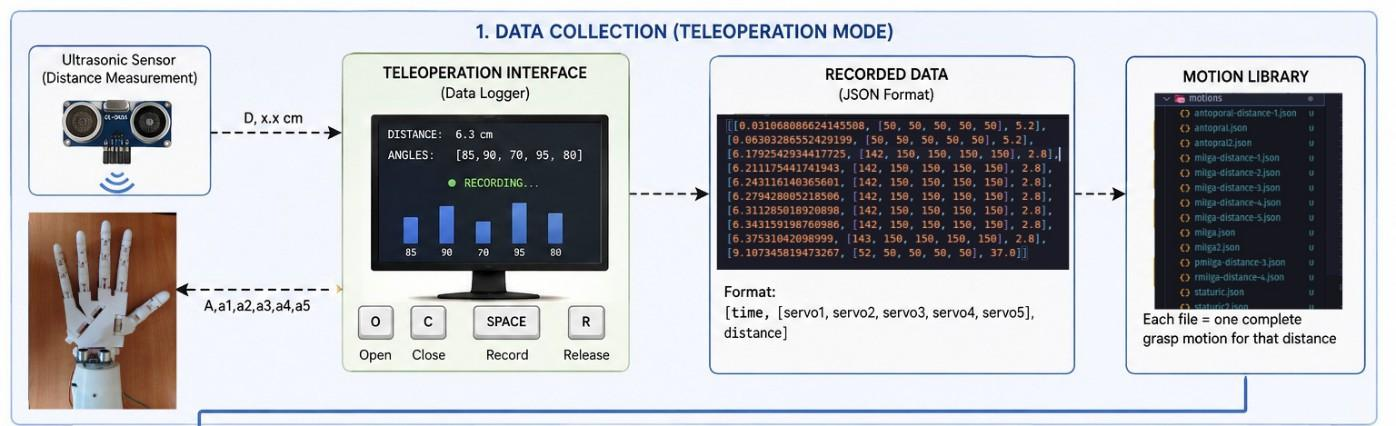
\includegraphics[width=5.38042in,height=1.64187in]{./media/image67.jpg}
\caption{APMS Architectural Phase 1: Data Collection and Trajectory Recording\label{fig:fig1}}
\end{figure}

During Phase 1 (Data Collection), hand gestures are captured via an IP
camera. The MediaPipe Hand Landmarker tracks landmarks and computes
finger extension ratios. Concurrently, an HC-SR04 ultrasonic distance
sensor records target distance. The calculated angles and distances are
serialized into JSON trajectory files, which populate the local Motion
Library.

\begin{figure}[htbp]
\centering
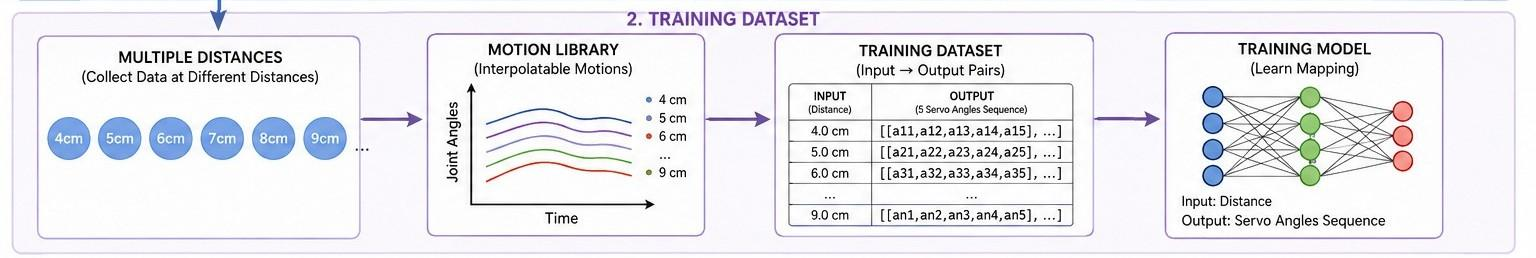
\includegraphics[width=5.28in,height=0.88687in]{./media/image35.jpg}
\caption{APMS Architectural Phase 2: Neural Network Trajectory Model Training\label{fig:fig2}}
\end{figure}

During Phase 2 (Model Training), the JSON files in the Motion Library
are parsed to construct a structured training database. A Multi-Layer
Perceptron (MLP) neural network is trained using backpropagation to
interpolate continuous joint trajectories for any distance within the
operational bounds (4.0 cm to 9.5 cm).

\begin{figure}[htbp]
\centering
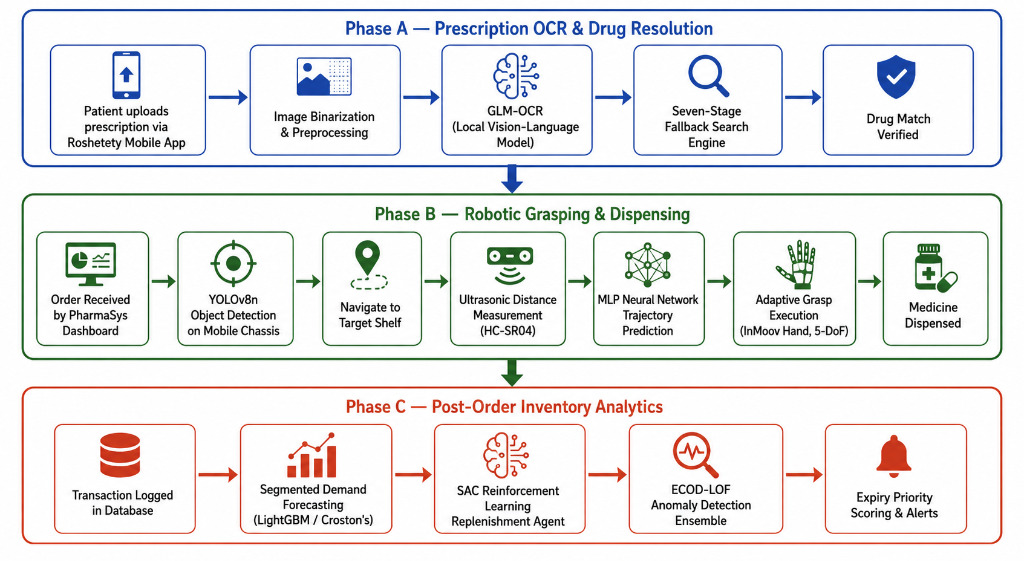
\includegraphics[width=5.34187in,height=1.225in]{./media/image29.jpg}
\caption{APMS Architectural Phase 3: Autonomous Grasping and Dispensing Execution\label{fig:fig3}}
\end{figure}

During Phase 3 (Autonomous Operation), the system functions
independently. The ultrasonic sensor measures the package distance,
which is filtered and checked for stability.

The MLP model generates the joint angles, driving the ESP32 to execute
the grasp. The camera captures the label, which is processed by local
GLM-OCR and matched against the reference database using the sequential
fallback engine before database inventory updates are completed.

\section{Subsystem Hardware Components
Overview}\label{subsystem-hardware-components-overview}

The physical dispensing hardware consists of four interconnected
components:

(a) MG995 Servos Assembly (b) Palm-mounted HC-SR04 Sensor

\begin{figure}[htbp]
\centering
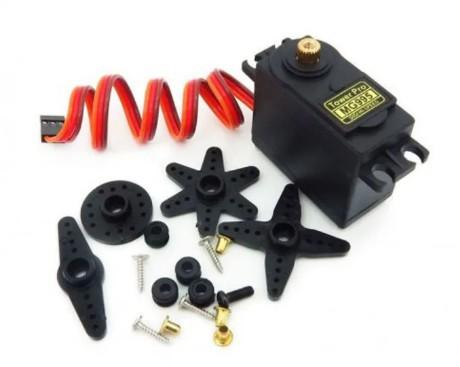
\includegraphics[width=2.25in,height=1.5in]{./media/image64.jpg}
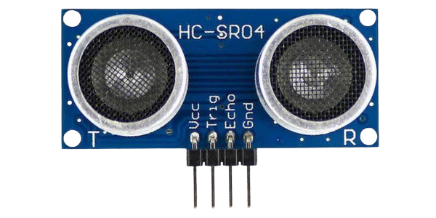
\includegraphics[width=2.25in,height=1.5in]{./media/image60.png}
\caption{APMS Hardware Integrations\label{fig:fig4}}
\end{figure}

\begin{itemize}
\item
  \textbf{InMoov Robotic Hand}: A 3D-printed anthropomorphic hand
  containing 5 MG995 metal gear servos mounted in the forearm. MG995
  servos provide a maximum torque of 12 kg\emph{$\cdot$}cm, driving finger
  flexion/extension via high-strength nylon tendons. The fingers operate
  within an experimental angular range of 50$^\circ$ (fully
  open) to 150$^\circ$ (fully closed).
\item
  \textbf{HC-SR04 Ultrasonic Distance Sensor}: Mounted on the palm of
  the hand to measure the distance to the target medicine pack
  (operational range: 4.0 cm to 9.5 cm). The sensor operates by emitting
  a 40 kHz ultrasonic pulse and measuring the echo return time, sampled
  at 50 Hz.
\item
  \textbf{ESP32 Microcontroller}: Acting as the hardware interface. It
  samples the ultrasonic sensor and drives the five PWM servo signals.
  It communicates with the host PC via serial USB communication at
  115200 baud.
\item
  \textbf{IP Camera Module}: Captures a high-resolution video feed of
  the workspace for both MediaPipe hand tracking (Phase 1) and label
  capture (Phase 3).
\end{itemize}

\section{Mechanical Kinematics and Joint Mapping
Equations}\label{mechanical-kinematics-and-joint-mapping-equations}

\subsection{Kinematic Linkage
Analysis}\label{kinematic-linkage-analysis}

Each of the five fingers is modeled as a serial kinematic chain
containing three revolute joints: the Metacarpophalangeal (MCP) joint,
the Proximal Interphalangeal (PIP) joint, and

the Distal Interphalangeal (DIP) joint. In the InMoov mechanical hand,
the PIP and DIP joints are coupled via a shared tendon linkage. When the
actuator pulls the tendon, both joints flex simultaneously, reducing the
active Degrees of Freedom (DoF) from 15 in a human hand to 5 active DoFs
in the robot (one servo per finger). Wrist pitch and twist represent an
additional 2 DoFs. Denavit-Hartenberg (D-H) coordinate frames are
established at each knuckle to trace the fingertip trajectories relative
to the base wrist frame.

\begin{figure}[htbp]
\centering
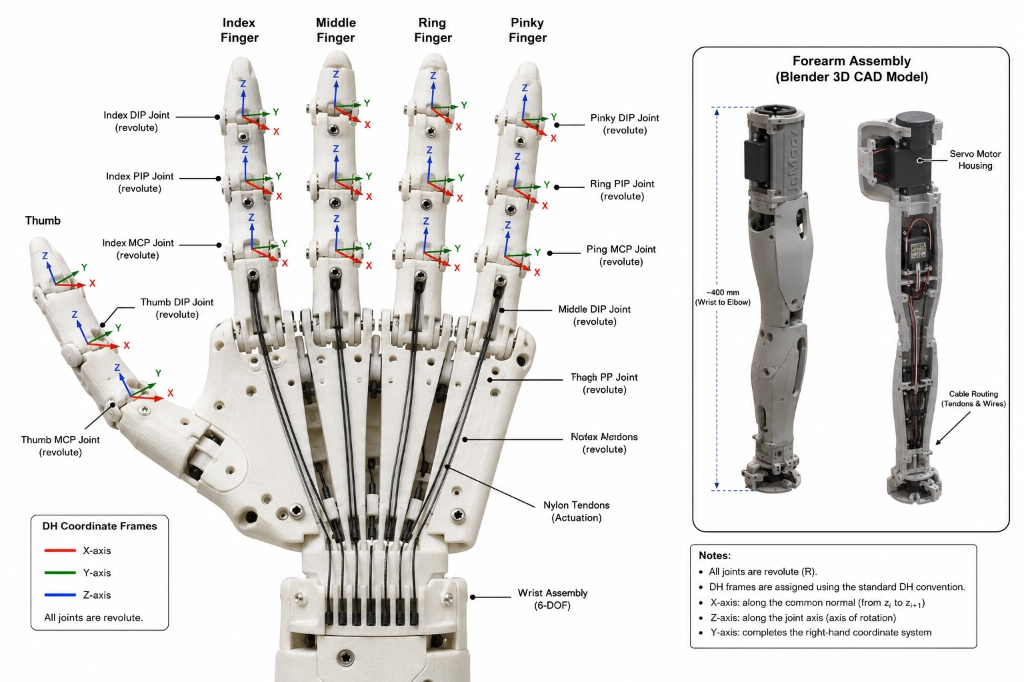
\includegraphics[width=3.00625in,height=1.34375in]{./media/image80.jpg}
% 
\includegraphics[width=2.93614in,height=2.93614in]{./media/image18.png}
\caption{Robotic Kinematics and Blender 3D Design: (a) DH Coordinate Frames (b) Blender Forearm Assembly View\label{fig:fig5}}
\end{figure}

\subsection{Finger-to-Servo Joint Mapping Equations}
\label{finger-to-servo-joint-mapping-equations}

To perform mimicry, the joint angles are computed from MediaPipe landmarks. We define the normalized extension ratio $R_i$ for finger $i$ based on the Euclidean distance from the fingertip to the wrist, normalized by the distance from the Metacarpophalangeal (MCP) knuckle to the wrist:

\begin{equation}
R_i = \frac{\|\mathbf{p}_{\text{tip},i} - \mathbf{p}_{\text{wrist}}\|}{\|\mathbf{p}_{\text{MCP},i} - \mathbf{p}_{\text{wrist}}\|}
\end{equation}

The target PWM command angle $A_i$ (constrained between fully open $A_{\text{open}} = 50^\circ$ and fully closed $A_{\text{closed}} = 150^\circ$) is calculated using a linear clamp-and-scale inversion mapping:

\begin{equation}
A_i = \text{clamp}\left( A_{\text{closed}} - \frac{R_i - R_{i,\min}}{R_{i,\max} - R_{i,\min}} \times (A_{\text{closed}} - A_{\text{open}}), \, A_{\text{open}}, \, A_{\text{closed}} \right)
\end{equation}

where $R_{i,\min}$ and $R_{i,\max}$ represent the calibration limits of the operator's finger extension. This normalization allows the system to remain invariant to the user's physical hand size.
\subsection{3D Printing Infill Density
Selection}\label{d-printing-infill-density-selection}

To manufacture the robotic hand, Blender was utilized to assemble,
verify tolerances, and repair STL meshes. The 3D printing parameters are
critical: printing with a high infill density (70\% to 100\%) increases
the mass of moving components, overloading the MG995 servos and
increasing power consumption. Conversely, very low infill
(\emph{\textless{}}15\%) leads to mechanical

failure under grasp load. Research in FDM tensile strength demonstrates
that structural resistance plateaues above 30\% infill density.

We deployed a segmented infill strategy:

\begin{itemize}
\item
  \textbf{Fingers and Phalanges}: Grid pattern at 25\% infill, balancing
  low inertia with high wall rigidity (1.6 mm walls prevent buckling
  under flexion stress).
\item
  \textbf{Palm Plate}: Gyroid pattern at 30\% infill, providing
  isotropic load resistance to absorb multi-directional grip forces.
\item
  \textbf{Forearm Housing}: Rectilinear pattern at 20\% infill,
  minimizing weight since it serves primarily as a protective shell.
\item
  \textbf{Wrist Gear Train}: Cubic subdivision pattern at 35\% infill to
  support gear teeth shear stresses.
\end{itemize}

This design achieved a 35\% to 40\% weight reduction compared to fully
dense parts, keeping motor loads well within the 12 kg\emph{$\cdot$}cm rated
torque.

\begin{figure}[htbp]
\centering
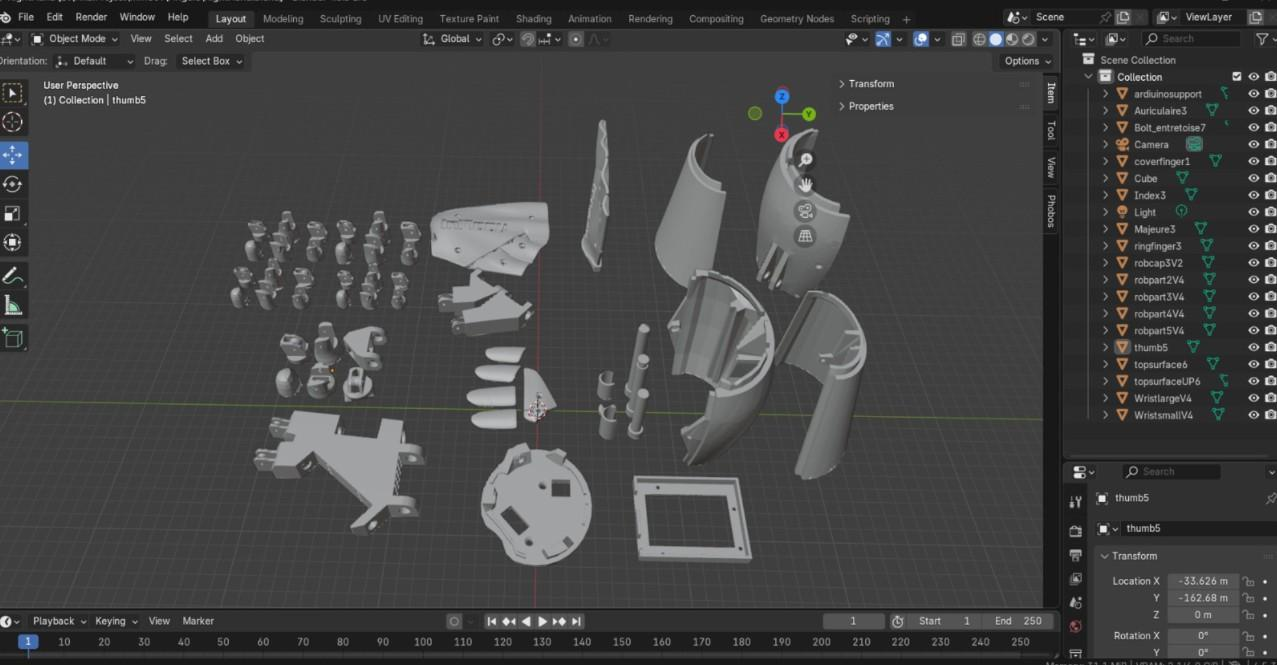
\includegraphics[width=4.20313in,height=2.17644in]{./media/image73.jpg}
\caption{3D-Printed Components: High-Level and Low-Level Exploded Assembly View\label{fig:fig6}}
\end{figure}

\section{Software Clean Architecture and Database
Design}\label{software-clean-architecture-and-database-design}

The automated pharmacy management system software infrastructure
connects the interfaces, the relational database, and the hardware.

(a)Figure: Flutter Clean Architecture (b)Figure: Backend Architecture

\begin{figure}[htbp]
\centering
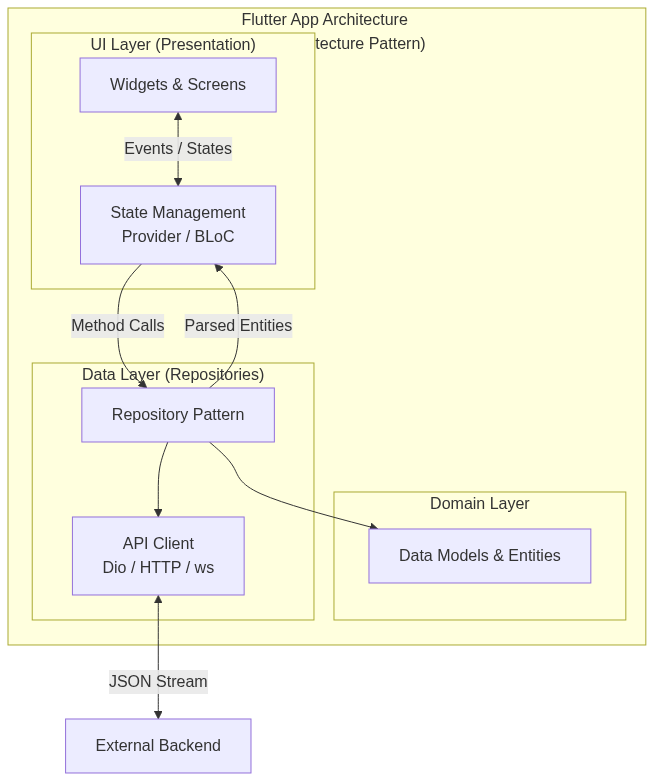
\includegraphics[width=2.74082in,height=3.44912in]{./media/image17.png}
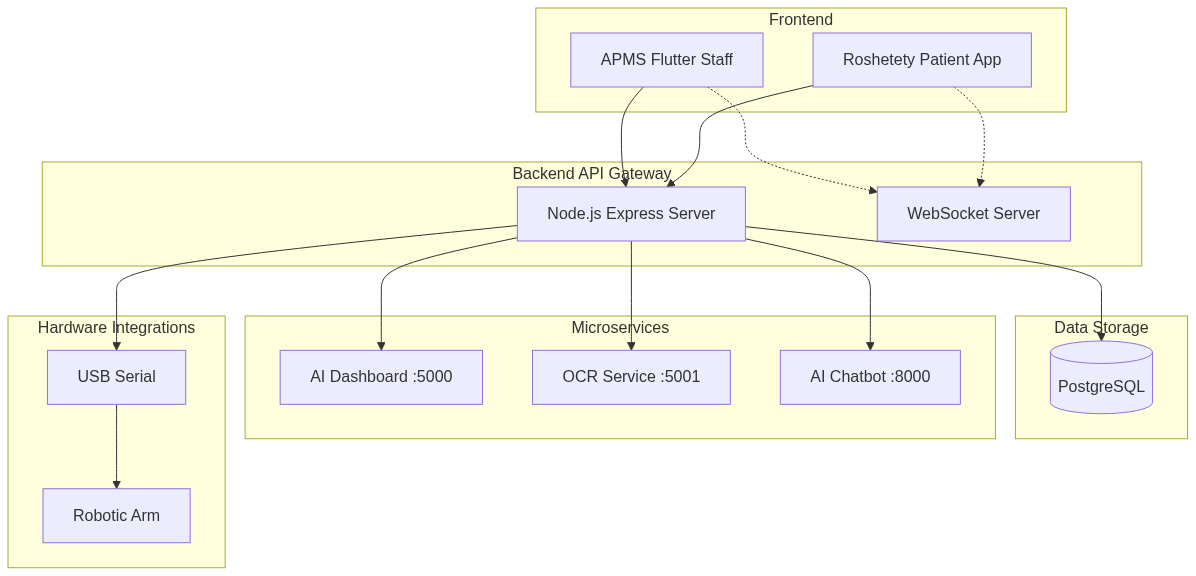
\includegraphics[width=4.00521in,height=2.44593in]{./media/image68.png}
\caption{APMS Software Subsystem Design\label{fig:fig7}}
\end{figure}

\textbf{Frontend Implementation}: The frontend is developed using
Flutter (Dart), enabling natively compiled cross-platform applications
from a single codebase based on Clean Architecture principles.

\begin{itemize}
\item
  \textbf{PharmaSys Staff Dashboard} The PharmaSys app is organized into
  a clean, feature-based architecture. It implements a responsive design
  approach using LayoutBuilder to seamlessly switch between Desktop
  (multi-column grid with sidebar navigation), Tablet, and Mobile
  layouts. State management is handled via Provider, ensuring
  lightweight and efficient UI updates. A comprehensive API Service
  Client manages all HTTP requests, featuring custom exception classes,
  timeout management, offline detection, and a dedicated WebSocket
  client for real-time robotic hardware updates.
\item
  \textbf{Roshetety Patient App} The patient app follows a flat
  navigation model optimized for minimal friction. It includes full
  Arabic/English bilingual support using Flutter\textquotesingle s
  Directionality widget for Right-to-Left (RTL) layout switching. A live
  WebSocket connection provides patients with real-time order tracking
  updates (Pending $\rightarrow$ Processing $\rightarrow$ Dispensed $\rightarrow$ Ready).
\end{itemize}

\textbf{Database Implementation}: The system relies on a PostgreSQL
relational database designed to guarantee data integrity, historical
accuracy, and efficient querying. The schema comprises core tables
designed for normalized efficiency:

\begin{itemize}
\item
  users: Manages staff authentication and role-based access.
\item
  medicines\_inventory: The central repository tracking trade names,
  active substances, stock levels, costs, and expiration dates.
\item
  invoices\_fawateer \& invoice\_items: Tracks supplier deliveries and
  financial payables.
\item
  prescriptions \& prescription\_items: Manages patient orders, linking
  requested items directly to the physical inventory. The database is
  accessed via the pg (node-postgres) driver utilizing connection
  pooling to ensure high-throughput performance during peak pharmacy
  hours.
\end{itemize}

\begin{figure}[htbp]
\centering
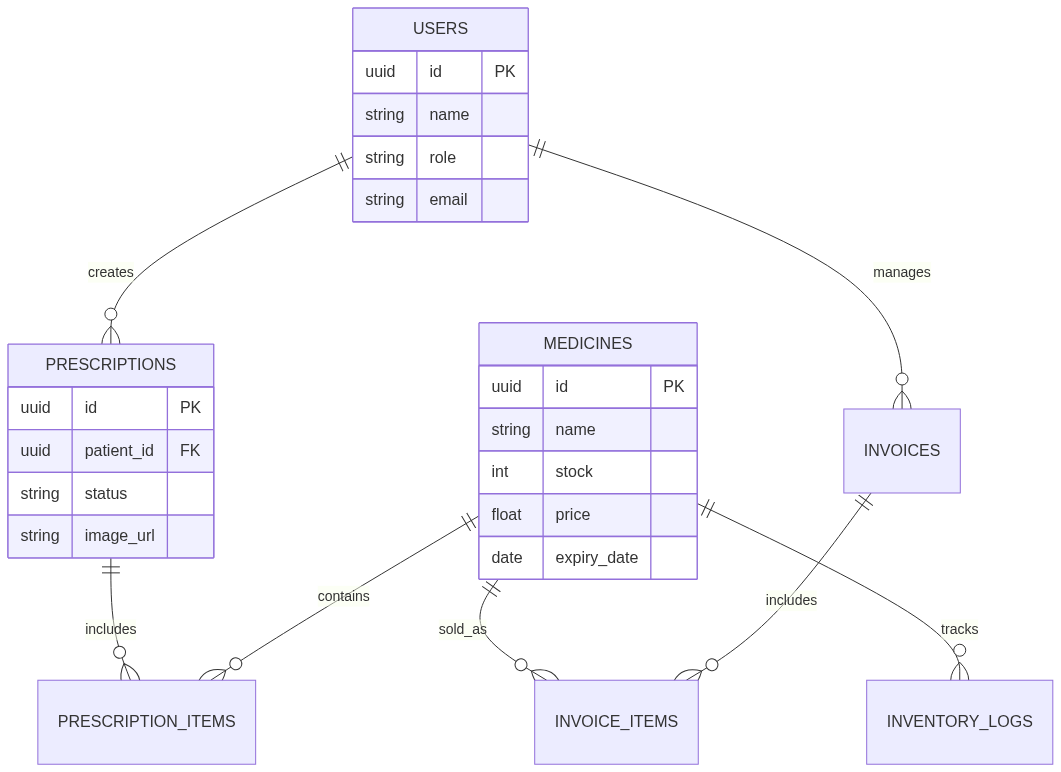
\includegraphics[width=3.0971in,height=2.23997in]{./media/image21.png}
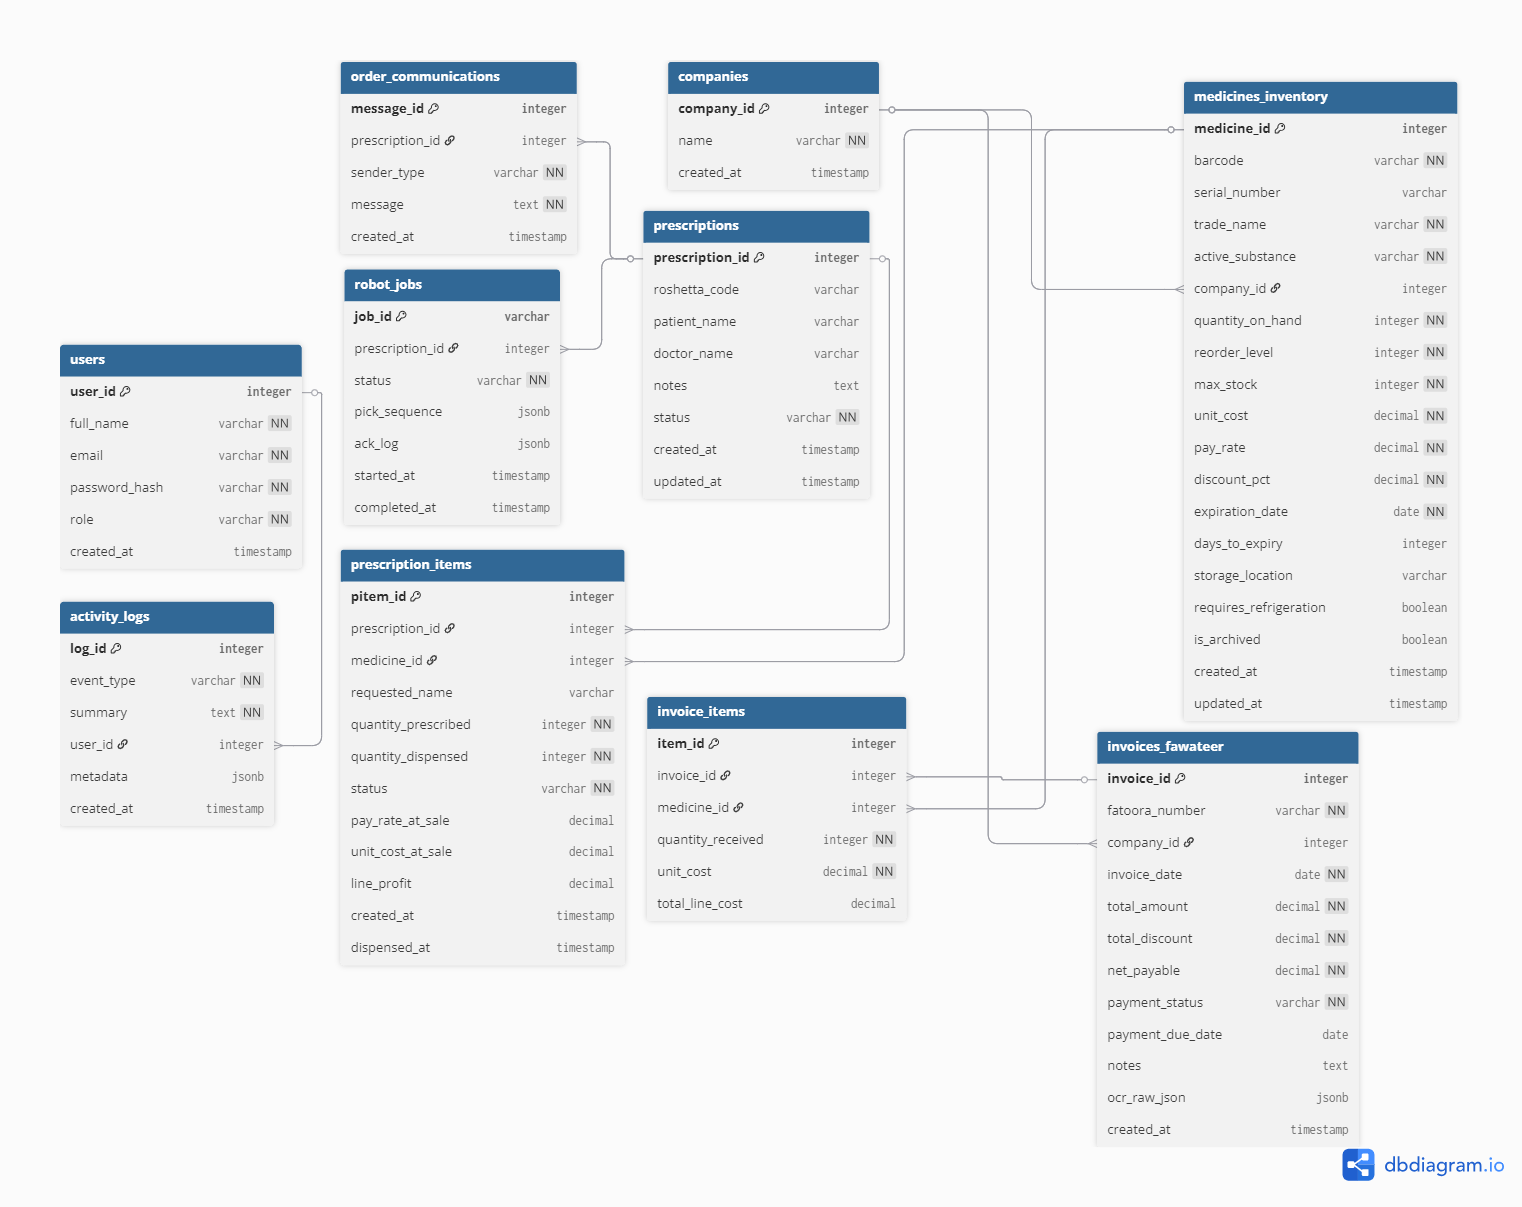
\includegraphics[width=3.60782in,height=2.16469in]{./media/image4.png}
\caption{Database ER Diagram Figure: Database Schema\label{fig:database_er_diagram}}
\end{figure}

\textbf{Backend Implementation}: The backend gateway is built using
Node.js and Express 5.x with TypeScript, adopting a modular three-tier
microservices architecture. It acts as the central hub connecting the
Flutter frontends, the PostgreSQL database, and the physical hardware.

\textbf{API Gateway Architecture}: The Express server features a modular
router architecture separating concerns (Auth, Medicines, Invoices,
Prescriptions, Robot).

\begin{itemize}
\item
  Authentication \& Security: Implemented via JSON Web Tokens (JWT) and
  bcryptjs for password hashing. Role Guards strictly differentiate
  between Staff and Manager endpoints.
\item
  Validation: Request body validation is strongly typed using the zod
  library.
\item
  File Processing: Utilizes multer for multipart uploads and xlsx for
  bulk Excel data imports.
\end{itemize}

\begin{figure}[htbp]
\centering
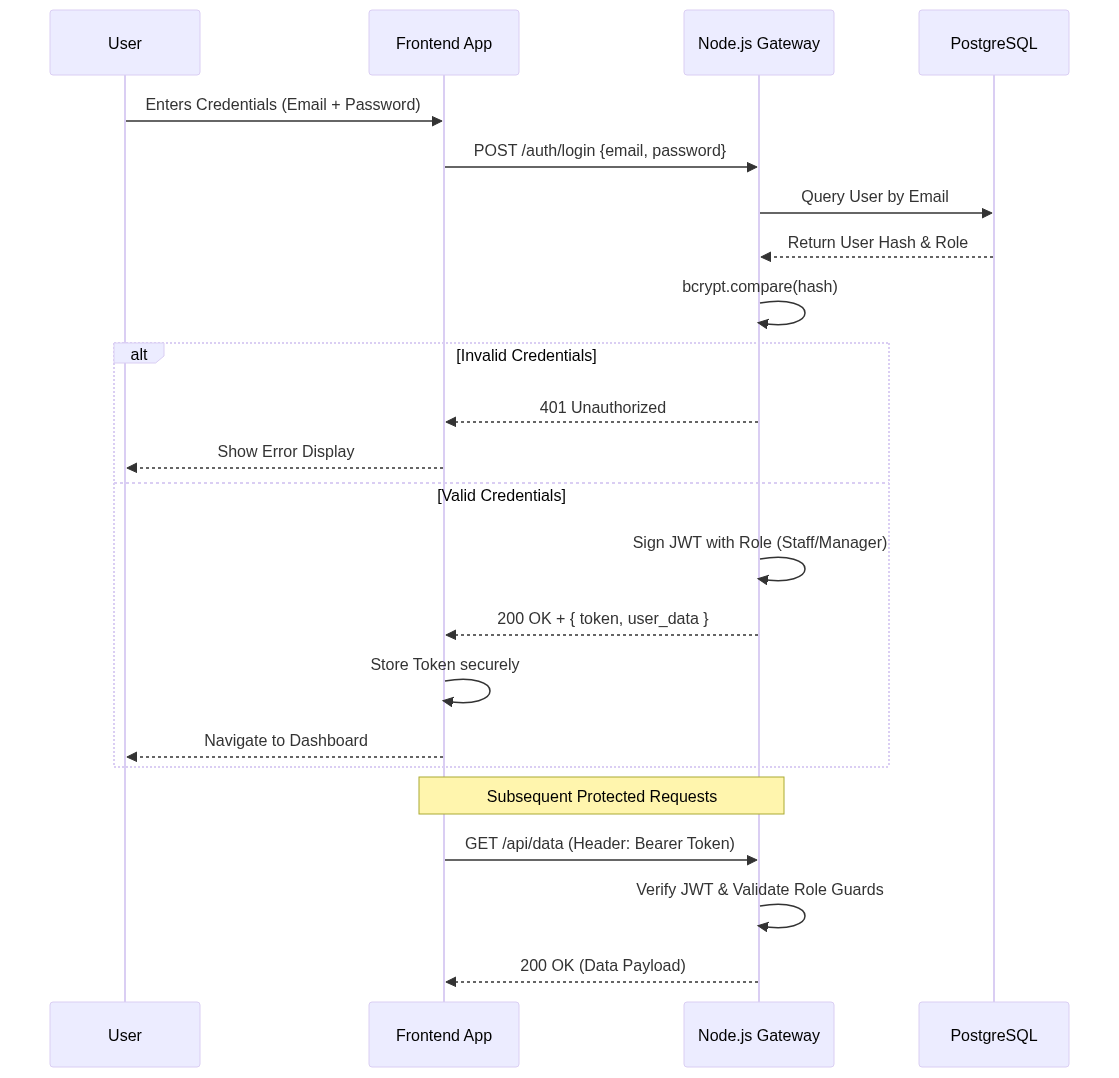
\includegraphics[width=4.18073in,height=4.00602in]{./media/image23.png}
\caption{Security Authentication Flow\label{fig:security_authentication_flow}}
\end{figure}

\section{UI/UX and HCI Design}\label{uiux-and-hci-design}

The UI/UX design methodology for both the PharmaSys Staff Dashboard and
the Roshetety Patient Application is strictly grounded in established
Human-Computer Interaction (HCI) principles. The design was informed by
the specific cognitive and environmental demands of pharmacy work, such
as high time pressure and frequent interruptions.

\begin{figure}[htbp]
\centering
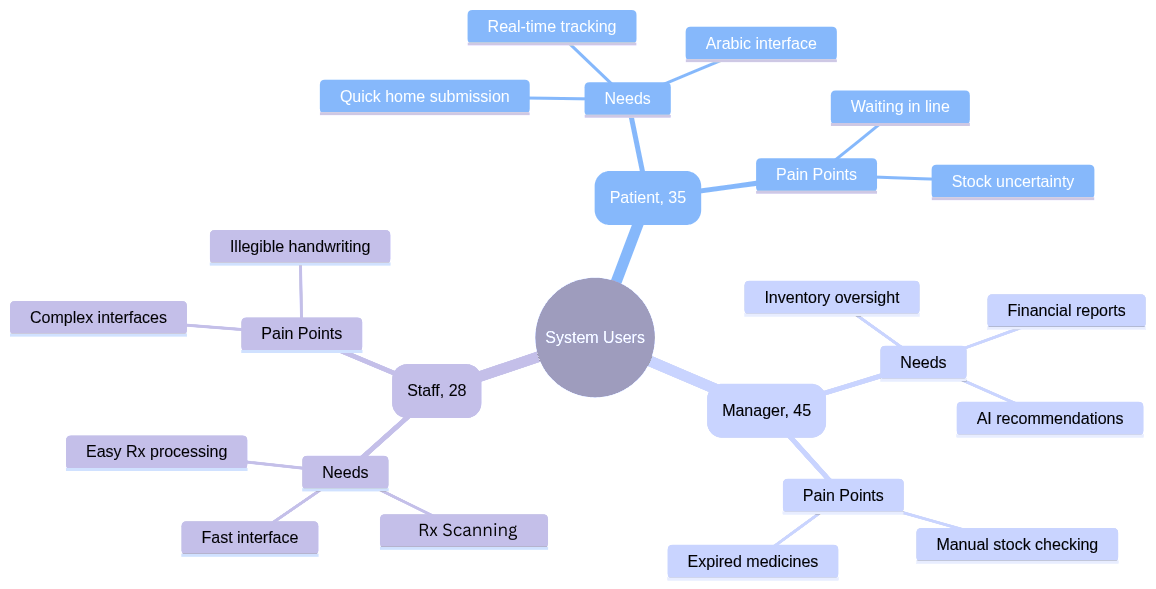
\includegraphics[width=5.36593in,height=2.70245in]{./media/image33.png}
\caption{User Personas\label{fig:user_personas}}
\end{figure}

\begin{figure}[htbp]
\centering
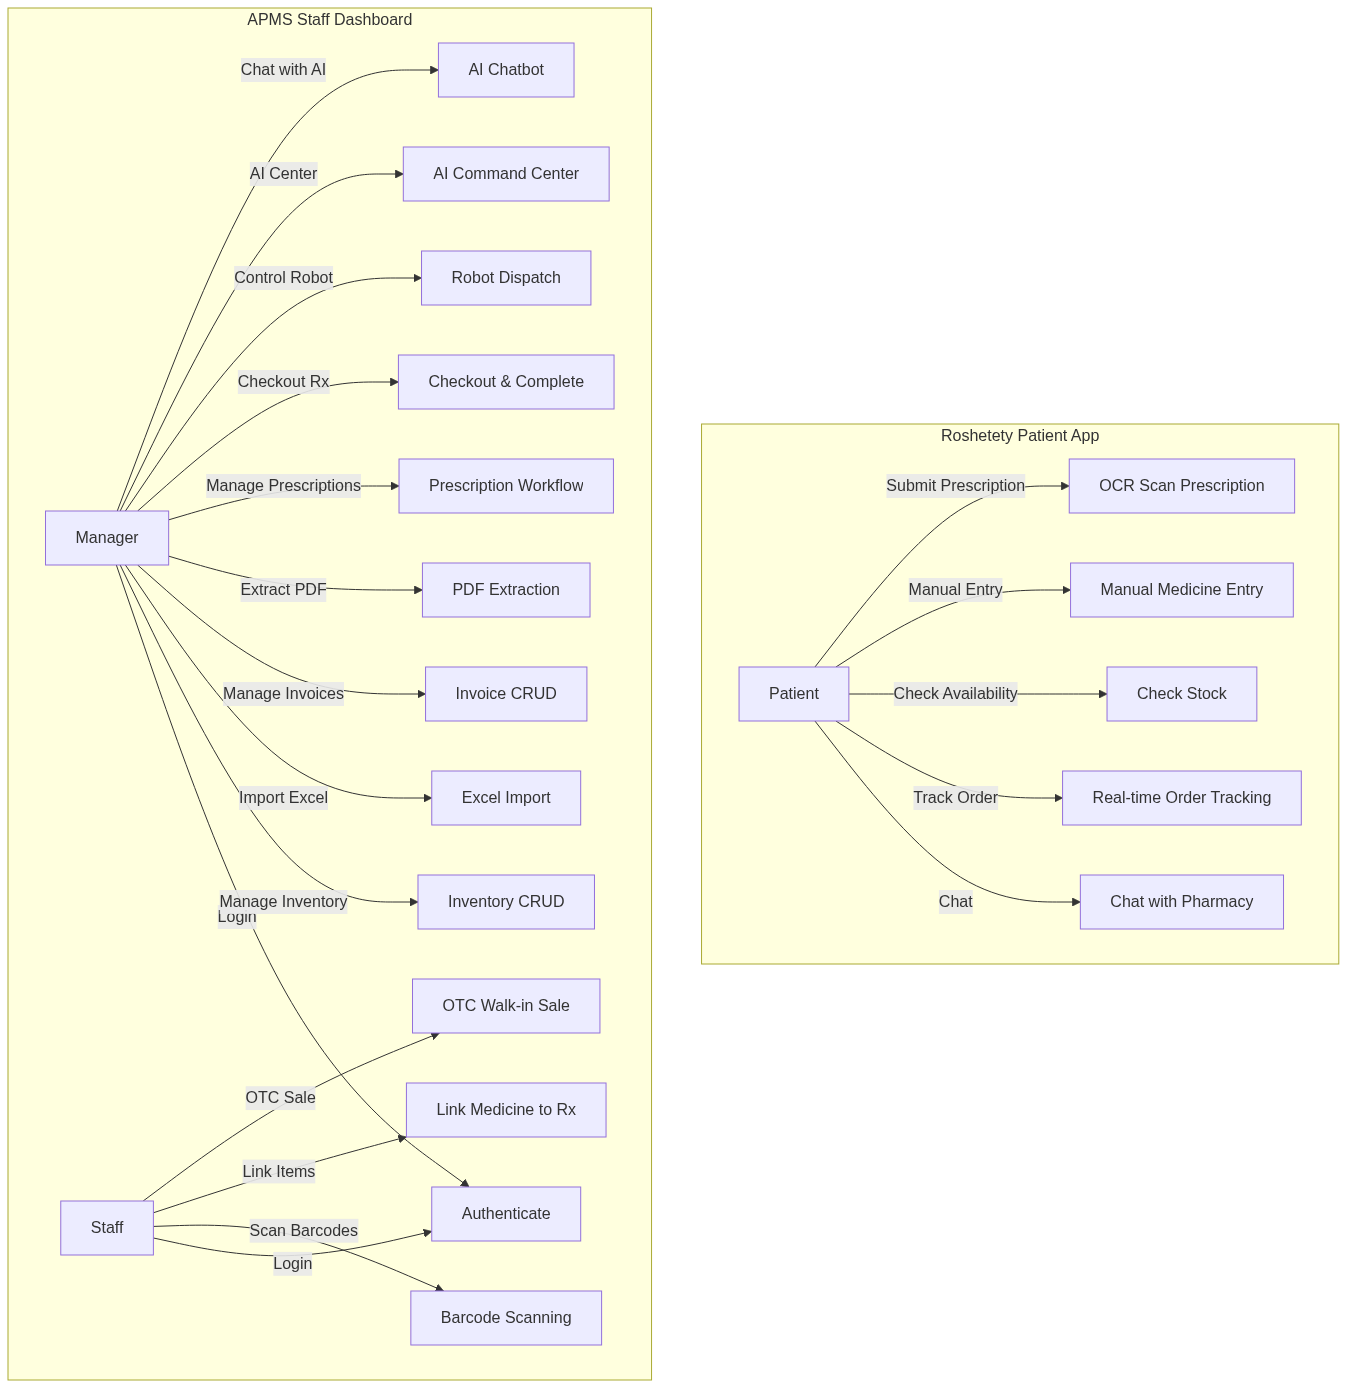
\includegraphics[width=5.52771in,height=5.72396in]{./media/image37.png}
\caption{System Use Cases\label{fig:system_use_cases}}
\end{figure}

\textbf{User Research and Interviews}: To ensure the interface met the
operational reality of Egyptian community pharmacies, a series of
structured interviews were conducted with three pharmacy managers and
five pharmacy staff members. The feedback collected highlighted several
core pain points:

\begin{itemize}
\item
  High Cognitive Load: Staff reported that existing software required
  too many clicks to complete a single sale, leading to user fatigue.
\item
  Screen Clutter: Managers complained that crucial data (like low stock
  alerts) was often buried under menus.
\item
  Physical Constraints: Staff often operate the software while holding
  physical products or talking to patients, necessitating larger click
  targets and keyboard-navigable workflows. These insights directly
  translated into our User-Centered Design (UCD) approach. We
  implemented large touch targets ($\ge$ 44px), flattened the navigation
  hierarchy to minimize steps for common tasks like checking out a
  prescription, and introduced global keyboard shortcuts to speed up
  high-volume data
  entry.
\end{itemize}

\begin{figure}[htbp]
\centering
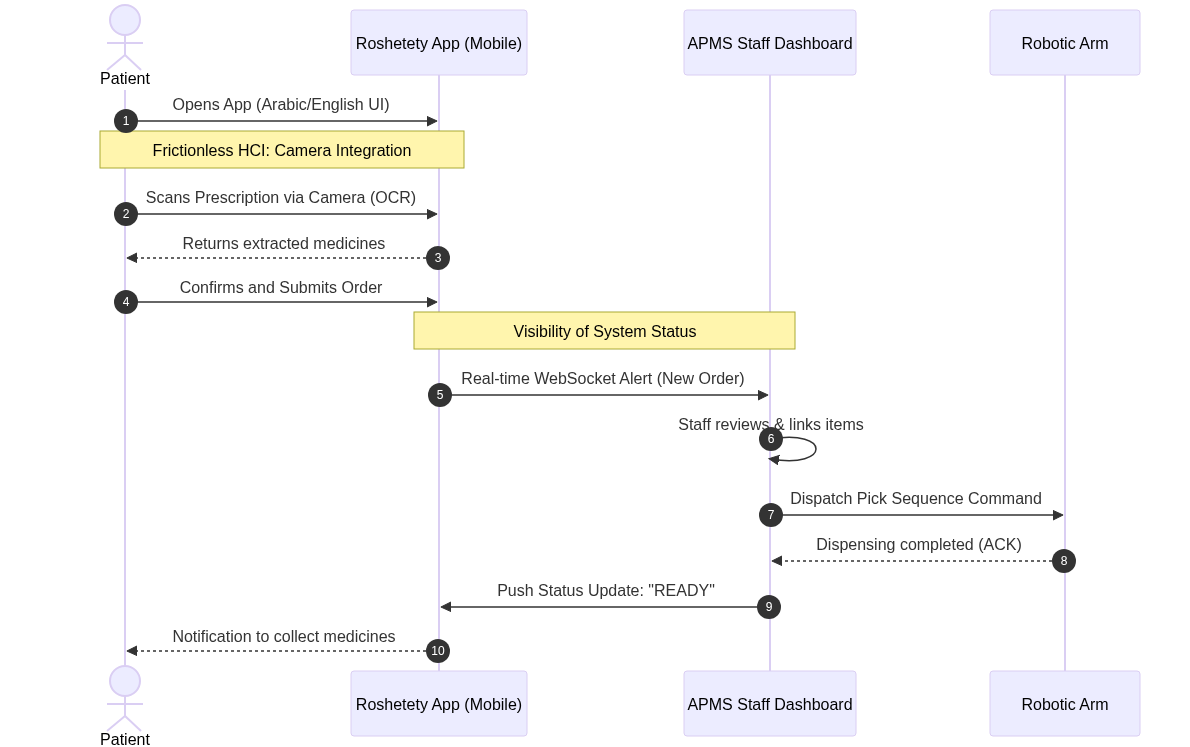
\includegraphics[width=5.42992in,height=3.42188in]{./media/image66.png}
\caption{User Journey Sequence\label{fig:user_journey_sequence}}
\end{figure}

\textbf{Design System and Tokens}: A comprehensive Design System was
established to guarantee visual consistency and reduce development
overhead. This system is driven by predefined "Design Tokens" that
control color, typography, and spacing across both the staff and patient
applications.

\begin{itemize}
\item
  Typography Strategy: The system employs a dual-font approach to
  support seamless bilingual (Arabic/English) interfaces. "Inter" is
  utilized for crisp English legibility, while "Cairo" ensures modern,
  highly readable Arabic text.
\item
  Color Palette: The PharmaSys staff dashboard utilizes a professional
  "Medical Blue" primary palette (\#02569B), designed to reduce eye
  strain during prolonged enterprise use. The Roshetety patient app
  utilizes a softer, more inviting aesthetic.
\item
  Accessibility and Status: Status indicators rely on redundant
  encoding---combining color, icons, and text labels---to ensure
  accessibility for color-blind users (e.g., a green checkmark for
  in-stock, an amber triangle for low stock, a red cross for expired
  items).
\end{itemize}

\begin{figure}[htbp]
\centering
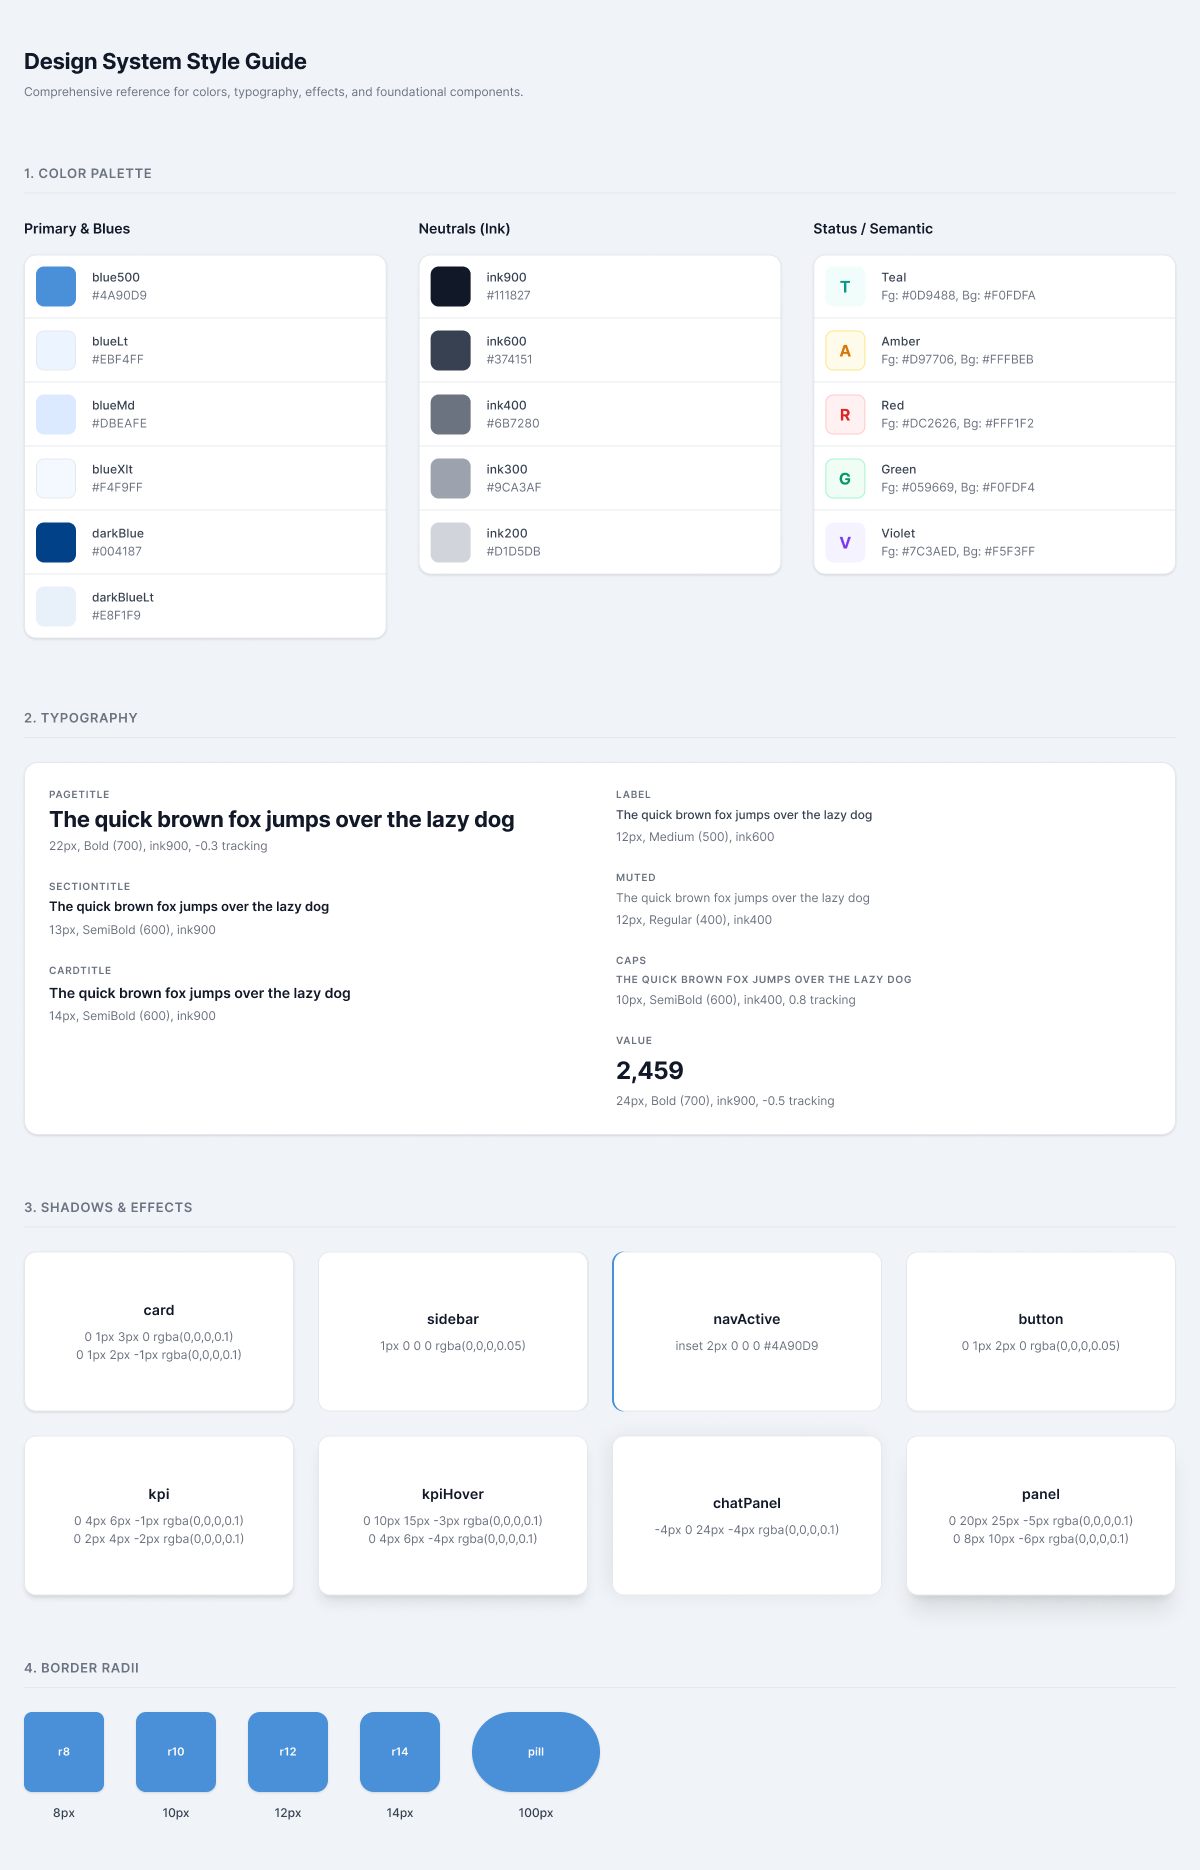
\includegraphics[width=4.01042in,height=2.3295in]{./media/image24.png}
\caption{Design System Tokens\label{fig:design_system_tokens}}
\end{figure}

\textbf{Visibility of System Status and Navigation}: Real-time
indicators are used throughout the system. Key Performance Indicator
(KPI) cards update dynamically, WebSocket badges show connection status,
and the robot control panel displays live arm status. The navigation
pattern relies on a collapsible sidebar, ensuring that the main
workspace is maximized for data-heavy views.

\begin{figure}[htbp]
\centering
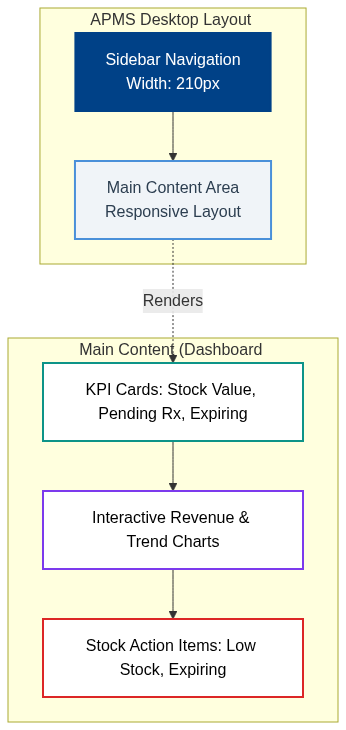
\includegraphics[width=1.80208in,height=2.77742in]{./media/image7.png}
\caption{Navigation Wireframe\label{fig:navigation_wireframe}}
\end{figure}

A summary of the APMS software technology stack is documented in Table~\ref{tab:tech_stack}.

\begin{table}[htbp]
    \centering
    \caption{APMS Technology Stack Overview}
    \label{tab:tech_stack}
    \vspace{0.5em}
    \small
    \begin{tabular}{ll p{3.2cm} p{5.5cm}}
        \toprule
        \textbf{Subsystem} & \textbf{Framework/Tech} & \textbf{Component} & \textbf{Rationale} \\
        \midrule
        Frontends & Flutter (Dart) & PharmaSys \& Roshetety & Multi-platform compilation from a single codebase. \\
        \addlinespace
        Backend & Node.js, Express & API Server gateway & Asynchronous event loop, rapid JSON handling. \\
        \addlinespace
        Database & PostgreSQL & Relational Database & Relational consistency, native JSON support, connection pooling. \\
        \addlinespace
        OCR Engine & Ollama & GLM-OCR & Local execution ensures HIPAA patient data privacy. \\
        \addlinespace
        Search Index & Elasticsearch & Inverted n-gram indexing & Sub-millisecond approximate string retrieval. \\
        \addlinespace
        Microcontroller & ESP32 & Servo & High-frequency hardware PWM signal generation. \\
        \bottomrule
    \end{tabular}
\end{table}

\textbf{Integrations (Hardware \& Real-time Synchronization)} A critical
component of this methodology is the seamless integration between
software logic and external/hardware services.

\begin{itemize}
\item
  \textbf{Real-Time Synchronization via WebSockets} A standalone
  WebSocket server operates alongside the HTTP server to broadcast
  real-time events. For example, when a bulk inventory upload occurs via
  the fallback Google Sheets bridge, the backend parses the CSV,
  validates it, and triggers a WebSocket broadcast. This allows the
  staff dashboard to instantly refresh the inventory view without manual
  page reloads.
\item
  \textbf{Robotic Arm Hardware Integration} The backend integrates
  directly with a robotic dispensing arm via a USB Serial Port (RS-232).
  When pharmacy staff dispatch a prescription, the backend generates a
  specific JSON pick sequence. This payload is transmitted over the
  serial port using the serialport Node.js package. The Arduino Mega
  micro-controller processes the command, drives the stepper motors to
  the specified bin, dispenses the medicine, and sends an
  Acknowledgement (ACK) back through the serial interface. The Node.js
  server receives this ACK, updates the PostgreSQL database, and
  instantly broadcasts the status change via WebSockets to both the
  staff dashboard and the patient\textquotesingle s mobile app
\end{itemize}

\begin{figure}[htbp]
\centering
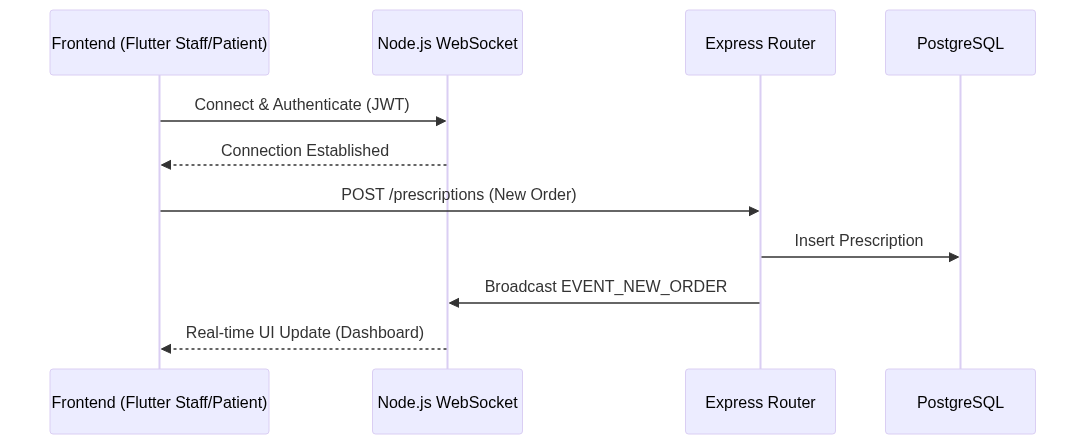
\includegraphics[width=6.13021in,height=2.5157in]{./media/image28.png}
\caption{WebSocket Sequence\label{fig:websocket_sequence}}
\end{figure}

\section{System Initialization Bootstrap
Sequence}\label{system-initialization-bootstrap-sequence}

The system bootstrap module acts as the initialization orchestrator for
the entire pipeline, executing all intensive resource-loading operations
before the FastAPI server begins accepting requests. This ensures
minimal response latency. The bootstrap sequence consists of three
sequential steps:

\begin{enumerate}
\def\labelenumi{\arabic{enumi})}
\item
  \textbf{Step 1: Resource Loading (init\_search())}: Loads the unified
  drug database CSV file into a pandas DataFrame, loads the FAISS index
  and pre-computed embeddings from disk, initializes the
  SentenceTransformer model in memory, builds the Python set lookup
  structure for exact matching, and establishes the connection pool to
  Elasticsearch.
\item
  \textbf{Step 2: Model Availability Check}: Performs a local HTTP
  health check on the Ollama API to verify that the GLM-OCR model is
  running, loaded, and responsive.
\item
  \textbf{Step 3: FastAPI Port Binding}: Binds the application to the
  configured host port, initializing the REST endpoints and WebSocket
  channels with all resources fully preloaded.
\end{enumerate}

\section{AI Models Design and Analytics
Architecture}\label{ai-models-design-and-analytics-architecture}

The background intelligence layer running in the APMS backend contains
four distinct models:

\begin{figure}[htbp]
\centering
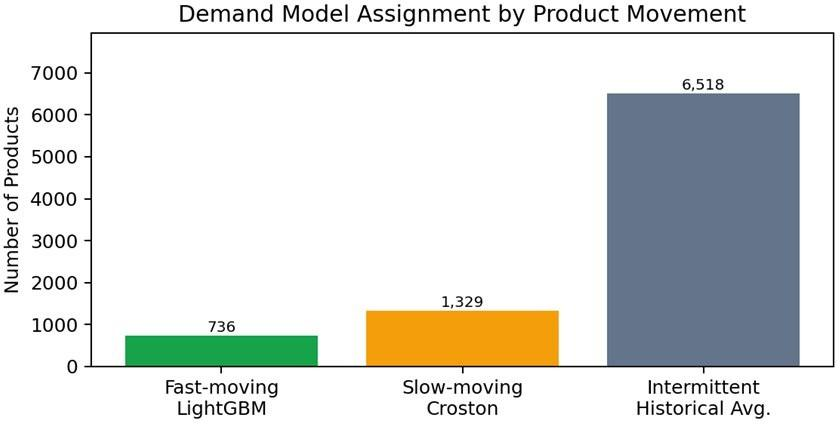
\includegraphics[width=4.8125in,height=2.42917in]{./media/image78.jpg}
\caption{Product Segmentation Pipeline for Demand Forecasting\label{fig:fig8}}
\end{figure}

\begin{enumerate}
\def\labelenumi{\arabic{enumi})}
\item
  \textbf{Segmented Demand Forecasting}: Products are divided into three
  segments: Fast-Moving, Slow-Moving, and Intermittent. Fast-moving
  items are modeled using a LightGBM regressor trained on engineered
  features (historical lag variables of 1, 2, 3, 6, and 12 months,
  rolling means, trend variables, and cyclical month encodings).
  Slow-moving items are modeled using Croston's Method, which separately
  forecasts demand sizes and inter-demand intervals. Intermittent items
  with sparse sales are assigned a 12-month historical trailing average
  baseline.
\item
  \textbf{Expiry Priority Scoring}: Computes a composite risk score for
  all inventory lines:
\end{enumerate}

\emph{S} = 0\emph{.}45\emph{$\times$S}\textsubscript{expiry}
+0\emph{.}25\emph{$\times$S}\textsubscript{value}
+0\emph{.}15\emph{$\times$S}\textsubscript{coverage}
+0\emph{.}10\emph{$\times$S}\textsubscript{demand}
+0\emph{.}05\emph{$\times$I}\textsubscript{warning} (3)

where \emph{S}\textsubscript{expiry} is inversely proportional to days
to expiry, \emph{S}\textsubscript{value} represents the financial value
at risk, \emph{S}\textsubscript{coverage} represents current stock
coverage, \emph{S}\textsubscript{demand} represents historical velocity,
and \emph{I}\textsubscript{warning} is a binary flag triggered below 60
days. This score prioritizes clearance discounts (up to 40\% discount).

\begin{enumerate}
\def\labelenumi{\arabic{enumi})}
\setcounter{enumi}{2}
\item
  \textbf{Shift Anomaly Detection}: Monitors cash reconciliation logs.
  It uses expected cash, actual cash, expected/actual ratio, cash
  discrepancy, and weekday features. A non-parametric unsupervised
  ensemble of ECOD (Empirical Cumulative Distribution Outlier Detection)
  and LOF (Local Outlier Factor) detects cashier fraud or logging errors
  by requiring consensus between global density and local outlier
  models.
\item
  \textbf{SAC Replenishment Agent}: Formulates replenishment ordering as
  a Markov Decision Process (MDP) with a 5-dimensional state space:
\end{enumerate}

\emph{x\textsubscript{t}} = {[}\emph{I\textsubscript{t},
D\textsubscript{t}, V\textsubscript{t}, C\textsubscript{t},
R\textsubscript{t}}{]}\emph{\textsuperscript{T}} (4)

where \emph{I\textsubscript{t}} is stock on hand,
\emph{D\textsubscript{t}} is days since last order,
\emph{V\textsubscript{t}} is rolling demand, \emph{C\textsubscript{t}}
is coverage, and \emph{R\textsubscript{t}} is reorder ratio. The action
space is continuous (reorder quantity). The Soft Actor-Critic agent
maximizes cumulative reward:

\emph{R} = Revenue \emph{-} Ordering Cost \emph{-} Holding Cost \emph{-}
Stockout Penalty (5)

trained in a simulation environment calibrated on real historical
pharmacy transaction distributions.

\subsection{Croston's Method Mathematical Formulation}
\label{crostons-method-mathematical-formulation}

Croston's method separates the demand time-series into two distinct components: the non-zero demand size $z_t$ and the time interval between demands $p_t$. 

If demand $y_t > 0$ at time $t$, the estimates are updated as follows:
\begin{equation}
\hat{z}_t = \hat{z}_{t-1} + \alpha(y_t - \hat{z}_{t-1})
\end{equation}

\begin{equation}
\hat{p}_t = \hat{p}_{t-1} + \alpha(q - \hat{p}_{t-1})
\end{equation}

where $q$ represents the number of periods elapsed since the last non-zero demand, and $\alpha$ is a smoothing parameter (typically $0.1 \le \alpha \le 0.3$).

If demand $y_t = 0$ at time $t$, the estimates remain unchanged:
\begin{equation}
\hat{z}_t = \hat{z}_{t-1}
\end{equation}

\begin{equation}
\hat{p}_t = \hat{p}_{t-1}
\end{equation}

and the elapsed time counter is incremented:
\begin{equation}
q = q + 1
\end{equation}

The final demand forecast for any future horizon $h$ is predicted as the ratio of the components:
\begin{equation}
\hat{y}_{t+h|t} = \frac{\hat{z}_t}{\hat{p}_t}
\end{equation}

% \subsection{ECOD and LOF Anomaly
% Models}\label{ecod-and-lof-anomaly-models}

% ECOD is a fast, non-parametric anomaly detection algorithm that computes
% the empirical cumulative distribution function (ECDF) for each dimension
% \emph{d} of a sample \emph{x}:

% \uline{1}
% \textsuperscript{$\Sigma$}
\includegraphics[width=0.10417in,height=0.12153in]{./media/image49.png}

% \emph{F} (\emph{x} ) = I(\emph{x $\le$ x} )
% (11)
\includegraphics[width=\linewidth,height=0.12153in,keepaspectratio]{./media/image49.png}
\includegraphics[width=\linewidth,height=0.12153in,keepaspectratio]{./media/image49.png}
\includegraphics[width=0.14097in,height=0.17708in]{./media/image49.png}
\includegraphics[width=0.14375in,height=0.12153in]{./media/image49.png}
\includegraphics[width=\linewidth,height=0.12153in,keepaspectratio]{./media/image49.png}

% The anomaly score is calculated based on the tail probabilities:

% \emph{D}
\includegraphics[width=0.25139in,height=0.52917in]{./media/image49.png}

% \emph{O}(\emph{x}) = max (\emph{-} log
% \emph{F\textsubscript{d}}(\emph{x\textsubscript{d}})\emph{, -} log(1
% \emph{- F\textsubscript{d}}(\emph{x\textsubscript{d}}))) (12)

% \emph{d}=1

% which captures both left-tail and right-tail outliers.

% LOF measures the local density deviation of a data point relative to its
% neighbors. The local reachability density (lrd) of point \emph{p} is:

% lrd\emph{\textsubscript{k}}(\emph{p}) = $\Sigma$

% \emph{o}$\in$\emph{N\textsubscript{k}}(\emph{p})

% \emph{\textbar N\textsubscript{k}}(\emph{p})\emph{\textbar{}}

% reach-dist\emph{\textsubscript{k}}
\includegraphics[width=1.74097in,height=\textheight,keepaspectratio]{./media/image49.png}

% (13)

% (\emph{p, o})

% where \emph{N\textsubscript{k}}(\emph{p}) is the \emph{k}-distance
% neighborhood of \emph{p}, and
% reach-dist\emph{\textsubscript{k}}(\emph{p, o}) =
% max(\emph{d\textsubscript{k}}(\emph{o})\emph{, d}(\emph{p, o})). The LOF
% score is then:

% \textsuperscript{$\Sigma$}
% \uline{lrd\emph{\textsubscript{k}}(\emph{o})}
\includegraphics[width=1.46806in,height=0.25278in]{./media/image49.png}
\includegraphics[width=0.32569in,height=0.21181in]{./media/image49.png}
\includegraphics[width=0.28819in,height=0.21181in]{./media/image49.png}

% \emph{\textsuperscript{k} \textbar N}
% (\emph{p})\emph{\textbar{}}
\includegraphics[width=\linewidth,height=0.12153in,keepaspectratio]{./media/image49.png}

% An LOF score close to 1 indicates a normal point, while a score
% significantly greater than 1 indicates an outlier.

\subsection{ECOD [26] and LOF [27] Anomaly Models}
\label{ecod-and-lof-anomaly-models}

\subsubsection{Empirical Cumulative Distribution-Based Outlier Detection (ECOD)}
ECOD is a fast, non-parametric anomaly detection algorithm that computes the empirical cumulative distribution function (ECDF) for each dimension $d$ of a sample $x$. For a dataset of size $N$, the ECDF for dimension $d$ is defined as:
\begin{equation}
\hat{F}_d(x_d) = \frac{1}{N} \sum_{i=1}^{N} I(x_{i,d} \le x_d)
\end{equation}
where $I(\cdot)$ is the indicator function.

The anomaly score for a $D$-dimensional point $x$ is calculated based on the tail probabilities to capture both left-tail and right-tail outliers:
\begin{equation}
O(x) = \sum_{d=1}^{D} \max\left(-\log \hat{F}_d(x_d), -\log(1 - \hat{F}_d(x_d))\right)
\end{equation}

\subsubsection{Local Outlier Factor (LOF)}
LOF measures the local density deviation of a data point relative to its $k$-nearest neighbors. The local reachability density ($\text{lrd}$) of a point $p$ is defined as:
\begin{equation}
\text{lrd}_k(p) = \frac{|N_k(p)|}{\sum_{o \in N_k(p)} \text{reach-dist}_k(p, o)}
\end{equation}
where $N_k(p)$ is the $k$-distance neighborhood of $p$, and the reachability distance is given by:
\begin{equation}
\text{reach-dist}_k(p, o) = \max(d_k(o), d(p, o))
\end{equation}

The LOF score is then calculated as the average ratio of the $\text{lrd}$ of $p$'s neighbors to that of $p$:
\begin{equation}
\text{LOF}_k(p) = \frac{\sum_{o \in N_k(p)} \frac{\text{lrd}_k(o)}{\text{lrd}_k(p)}}{|N_k(p)|}
\end{equation}

An LOF score close to 1 indicates a normal inlier point, while a score significantly greater than 1 indicates an outlier.

\subsection{Model Hyperparameters}\label{model-hyperparameters}

The hyperparameter selections for the MLP trajectory generator and the
SAC replenishment agent are summarized below:

\begin{itemize}
\item
  \textbf{MLP Trajectory Model}: Dense input layer (1 node), 3 hidden
  layers (64, 128, 64 nodes with ReLU activation), and output layer (500
  nodes, representing 100 timesteps for 5 servos). Trained using the
  Adam optimizer (learning rate \emph{$\eta$} = 0\emph{.}001, batch size 32)
  over 500 epochs with Mean Squared Error (MSE) loss.
\item
  \textbf{SAC Agent}: Actor network with 2 hidden layers (256 nodes,
  ReLU) outputting mean and standard deviation of grasp sizes. Critic
  networks with 2 hidden layers (256 nodes, ReLU) modeling Q-values.
  Learning rate is 0\emph{.}0003, discount factor \emph{$\gamma$} =
  0\emph{.}99, and target update coefficient \emph{$\tau$} = 0\emph{.}005,
  utilizing a 1,000,000 transition capacity experience replay buffer.
\end{itemize}

\section{Prescription Dataset Collection and Ground Truth
Annotation}\label{prescription-dataset-collection-and-ground-truth-annotation}

To train, calibrate, and evaluate the prescription transcription
pipeline, we collected an authentic dataset of 500 physical
prescription papers from local polyclinics and community pharmacies
across Alexandria and Cairo, Egypt. These documents exhibit the diverse
handwriting styles, fading ink, non-standard cursive abbreviations, and
physical wrinkles typical of real-world clinical environments.

The dataset capture and preprocessing workflow proceeded as follows:

\begin{itemize}
\item
  \textbf{Image Acquisition}: High-resolution digital photographs of the
  prescriptions were captured using mid-range mobile phone cameras under
  three distinct ambient lighting levels: bright day/fluorescent
  lighting (250 lm), moderate room lighting (100 lm), and low-light
  evening setups (15 lm).
\item
  \textbf{Ground Truth Transcription}: To establish a rigorous baseline
  for evaluation, three licensed pharmacists independently transcribed
  each prescription. They manually extracted the brand name, active
  substance, dosage strength (e.g., 50 mg, 1 g), formulation type
  (tablet, syrup, injection), and dosage frequency instructions.
  Discrepancies between the transcribers were resolved via a majority
  consensus panel, resulting in a clean, standardized ground truth
  dataset.
\item
  \textbf{Reference Drug Directory}: In parallel, we built a local
  reference database containing 15,000+ drug brand and generic names.
  This database consolidated regional datasets from the Egyptian Drug
  Authority (EDA), U.S. FDA National Drug Code (NDC) Directory, and
  scraped web metadata from Vezeeta Egypt.
\end{itemize}

\section{OCR Model Selection and Comparison}\label{ocr-model-selection-and-comparison}

Selection of an appropriate OCR model was a critical design decision. Five candidates were evaluated against criteria relevant to Egyptian prescription processing: handwritten text recognition, medical text understanding, Arabic-English mixed content handling, context awareness, local deployment capability, API dependency, cost, and processing speed. Table~\ref{tab:table_ocr_comparison} presents a qualitative comparison.

\begin{longtable}[]{@{}
  >{\raggedright\arraybackslash}p{(\linewidth - 8\tabcolsep) * \real{0.25}}
  >{\raggedright\arraybackslash}p{(\linewidth - 8\tabcolsep) * \real{0.15}}
  >{\raggedright\arraybackslash}p{(\linewidth - 8\tabcolsep) * \real{0.15}}
  >{\raggedright\arraybackslash}p{(\linewidth - 8\tabcolsep) * \real{0.15}}
  >{\raggedright\arraybackslash}p{(\linewidth - 8\tabcolsep) * \real{0.15}}
  >{\raggedright\arraybackslash}p{(\linewidth - 8\tabcolsep) * \real{0.15}}@{}}
\caption{OCR Model Comparison — Qualitative Assessment\label{tab:table_ocr_comparison}}\\
\toprule
\textbf{Criterion} & \textbf{GLM-4} & \textbf{GPT-4V} & \textbf{Gemini} & \textbf{PaddleOCR} & \textbf{Tesseract} \\
\midrule
\endfirsthead
\toprule
\textbf{Criterion} & \textbf{GLM-4} & \textbf{GPT-4V} & \textbf{Gemini} & \textbf{PaddleOCR} & \textbf{Tesseract} \\
\midrule
\endhead
\bottomrule
\endlastfoot
Handwritten Text & Excellent & Excellent & Good & Good & Poor \\
Medical Understanding & High & High & High & Moderate & Low \\
Arabic-English Mixed & Strong & Strong & Strong & Moderate & Weak \\
Context Awareness & Full (LLM) & Full (LLM) & Full (LLM) & Limited & None \\
Local Deployment & Yes (Ollama) & No & No & Yes & Yes \\
API Dependency & None & Required & Required & None & None \\
Deployment Cost & Low & High & High & Low & Free \\
Processing Speed & Fast (local) & Moderate & Moderate & Fast & Fast \\
Suitability for Rx & Very High & High & High & Moderate & Low \\
\end{longtable}

\textbf{Selection Justification: GLM-4}

GLM-4, deployed locally via the Ollama platform, was selected for the following reasons:
\begin{itemize}
\item Its transformer-based vision-language architecture processes both visual and textual context simultaneously, enabling accurate recognition of handwritten characters even in degraded prescription images---a capability absent from conventional pipeline-based systems (Tesseract, PaddleOCR).
\item Local deployment via Ollama eliminates API latency, external dependencies, and per-query costs that cloud-based alternatives (GPT-4V, Gemini) would incur, which is critical for production pharmacy environments requiring consistent sub-10-second response times.
\item GLM-4 accepts carefully engineered system prompts that explicitly constrain extraction to English medicine names and suppress Arabic text, enabling deterministic, structured output with zero temperature.
\item GLM-4 provides strong Arabic-English mixed content handling---a property not exhibited by Tesseract or PaddleOCR---which is essential for Egyptian prescriptions where Arabic dosage instructions are interspersed with English drug names.
\end{itemize}

\section{OCR Pipeline}\label{ocr-pipeline}

\subsection{Image Preprocessing}\label{image-preprocessing}
Prescription images undergo a four-step preprocessing pipeline before OCR extraction. First, images are resized to 1600--2400 pixels on the long edge, balancing detail preservation with processing speed. Second, grayscale conversion eliminates color channel noise. Third, contrast enhancement at a factor of 1.8$\times$ sharpens text boundaries. Fourth, sharpening at 2.0$\times$ with unsharp mask filtering accentuates edge transitions. This sequence is ordered so that each operation works on progressively improved input. The pipeline adds sub-second overhead while providing an estimated 15--25\% improvement in OCR character accuracy.

\subsection{GLM-OCR Extraction}\label{glm-ocr-extraction}
The preprocessed image is submitted to GLM-4 via the Ollama API with engineered system and user prompts. The system prompt explicitly instructs the model to extract only English medicine names, ignore all Arabic text and dosage instructions, and return structured output with one medicine per line. Model parameters are configured for deterministic behavior: temperature 0.0, context window 512 tokens, maximum output 150 tokens, top-k 50, top-p 0.9, and repeat penalty 1.1. Zero temperature maximizes consistency; output limits prevent verbose responses that complicate parsing. A low-confidence auto-retry mechanism with refocus prompts handles transient extraction failures, subject to a maximum retry count.

\subsection{Text Normalization}\label{text-normalization}
Raw OCR output undergoes a seven-rule normalization pipeline: (1) Rx prefix stripping; (2) removal of 80+ dosage form words (tablet, capsule, syrup, suspension, drops, cream, gel, inhaler, ampoule, sachet, and Arabic transliterations); (3) standalone integer removal; (4) dosage frequency token removal; (5) Arabic character detection across five Unicode ranges, rejecting entries containing non-Latin script; (6) minimum length validation (at least 3 consecutive letters); (7) non-drug product blocklist filtering. This pipeline eliminates $>$ 95\% of dosage instructions, Arabic fragments, and non-drug content from search queries.

\section{OCR Core and Search Strategy
Selection}\label{ocr-core-and-search-strategy-selection}

When a prescription image is received by the APMS system, it undergoes
localized binarization and contrast adjustment before execution. A
local Vision-Language Model (GLM-OCR running offline via Ollama)
transcribes the cursive handwritten strokes. Due to the high rate of
spelling discrepancies in handwritten medical cursive, the raw text
cannot be queried directly in the relational database.

We selected and prioritized a \textbf{Seven-Stage Sequential Fallback
Search Engine} to resolve typographical noise, structured as follows:

\begin{enumerate}
\def\labelenumi{\arabic{enumi})}
\item
  \textbf{Stage 1: Exact Match}: Performs a direct, case-sensitive
  lookup on the local database. If the raw OCR output matches a
  registered trade name exactly, the system returns the item instantly
  with 100\% confidence, bypassing further processing.
\item
  \textbf{Stage 2: Normalized Match}: Strips punctuation, spaces,
  non-standard casing, and hyphens (e.g. ``mil-ga'' \emph{$\rightarrow$} ``milga''),
  running a fast set-membership query.
\item
  \textbf{Stage 3: Smart OCR Fix (Visual Confusion Correction)}:
  Substitutes character strings based on historical optical errors
  (e.g., cursive ``rn'' misread as ``m'', or vertical ``l'' misread as
  ``1'').
\item
  \textbf{Stage 4: Elasticsearch Indexing}: Queries an Elasticsearch
  node utilizing n-gram tokenization and inverted indexes, mapping
  matching components to trade names.
\item
  \textbf{Stage 5: Fuzzy Search (Jaro-Winkler Distance)}: Performs a
  character edit-distance query. It prioritizes differences near the end
  of strings to protect drug prefix similarity (e.g. distinguishing
  ``Milga'' from ``Miltown''). If a candidate scores \emph{$\ge$}
  0\emph{.}85, the loop exits.
\item
  \textbf{Stage 6: Semantic Search (Sentence-Transformers)}: Computes
  dense vector representations of the text, comparing cosine
  similarities against pre-computed embeddings of generic drug classes.
  This resolves severe handwriting distortions by capturing phonetic and
  therapeutic context.
\item
  \textbf{Stage 7: External Web Crawler Fallback}: Direct REST API
  requests query the live Vezeeta Egypt directory, catching recently
  registered or unindexed medications.
\end{enumerate}

\begin{figure}[htbp]
\centering
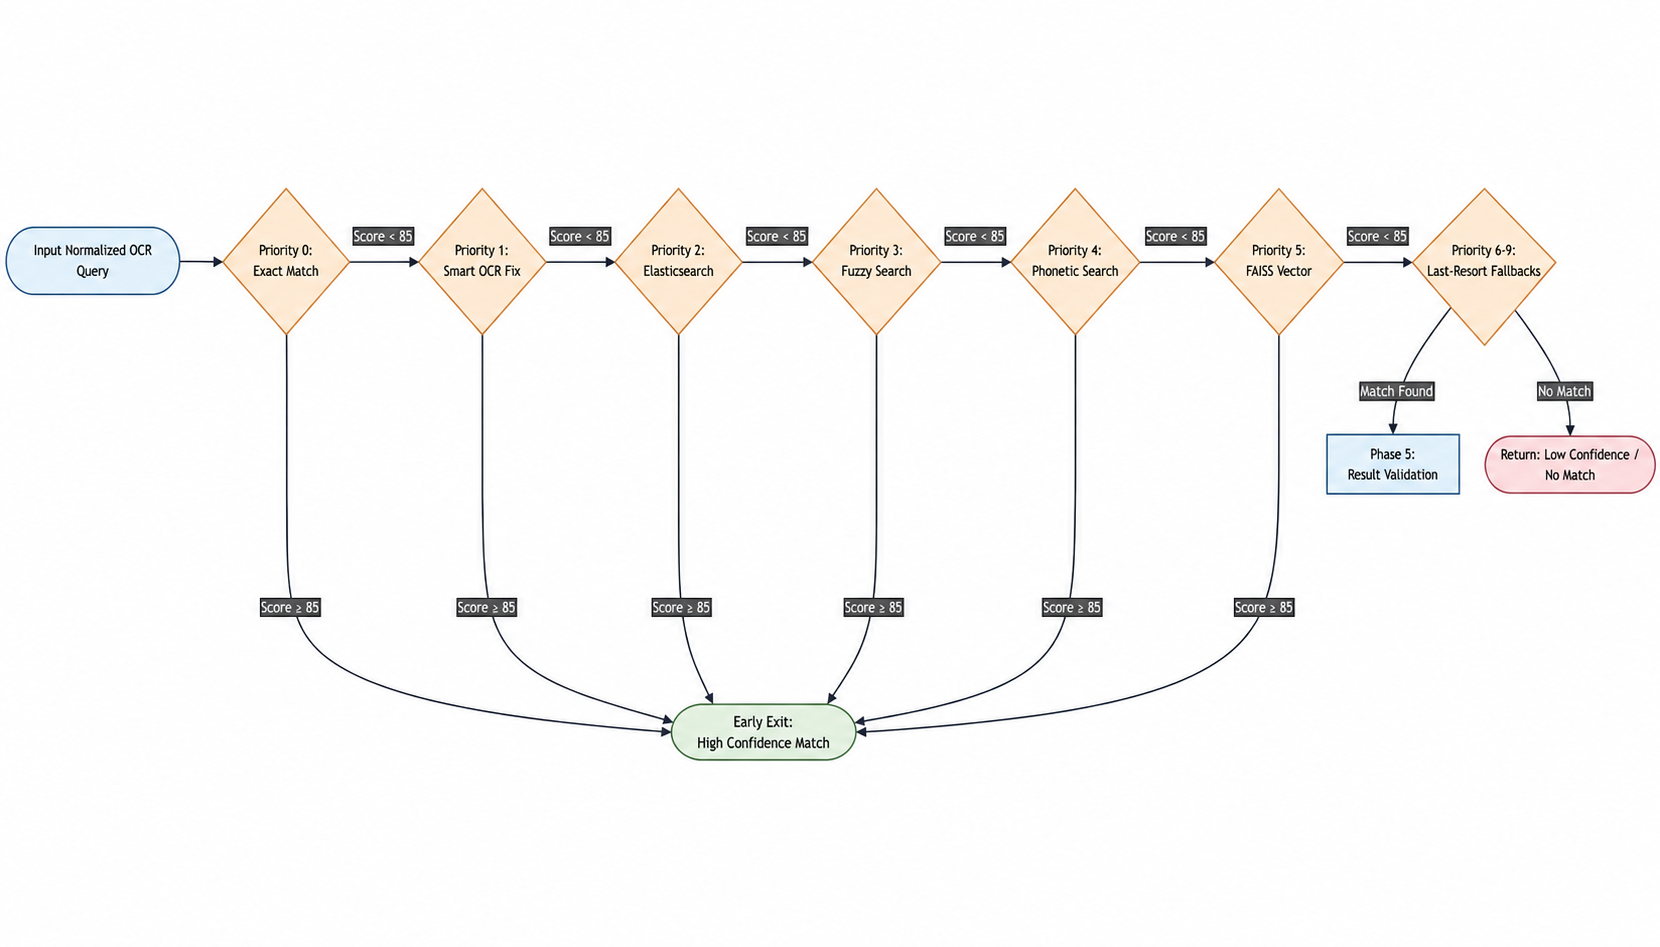
\includegraphics[width=5.00625in,height=3.36in]{./media/dem_fig.png}
\caption{Sequential Search Decision Tree with Early-Exit Confidence Thresholding\label{fig:fig9}}
\end{figure}

The characteristics and computational complexities of the search stages
are detailed in Table~\ref{tab:table5}.

\begin{longtable}[]{@{}
  >{\raggedright\arraybackslash}p{(\linewidth - 6\tabcolsep) * \real{0.0910}}
  >{\raggedright\arraybackslash}p{(\linewidth - 6\tabcolsep) * \real{0.1714}}
  >{\raggedright\arraybackslash}p{(\linewidth - 6\tabcolsep) * \real{0.1224}}
  >{\raggedright\arraybackslash}p{(\linewidth - 6\tabcolsep) * \real{0.5650}}@{}}
\caption{Search Method Characteristics\label{tab:table5}}\\

\toprule\noalign{}
\begin{minipage}[b]{\linewidth}\centering
\textbf{Priority}
\end{minipage} & \begin{minipage}[b]{\linewidth}\centering
\textbf{Method}
\end{minipage} & \begin{minipage}[b]{\linewidth}\centering
\textbf{Complexity}
\end{minipage} & \begin{minipage}[b]{\linewidth}\raggedright

\textbf{Justification for Priority Order}

\end{minipage} \\
\begin{minipage}[b]{\linewidth}\centering
0
\end{minipage} & \begin{minipage}[b]{\linewidth}\centering
Exact Match
\end{minipage} & \begin{minipage}[b]{\linewidth}\centering
\emph{O}(1)
\end{minipage} & \begin{minipage}[b]{\linewidth}\raggedright

Instant lookup, 100\% precision; matches 30--40\% of clear inputs

\end{minipage} \\
\begin{minipage}[b]{\linewidth}\centering
1
\end{minipage} & \begin{minipage}[b]{\linewidth}\centering
Normalized Match
\end{minipage} & \begin{minipage}[b]{\linewidth}\centering
\emph{O}(1)
\end{minipage} & \begin{minipage}[b]{\linewidth}\raggedright

Handles case/whitespace variations without expensive string metrics

\end{minipage} \\
\begin{minipage}[b]{\linewidth}\centering
2
\end{minipage} & \begin{minipage}[b]{\linewidth}\centering
Smart OCR Fix
\end{minipage} & \begin{minipage}[b]{\linewidth}\centering
\emph{O}(\emph{V} log \emph{N} )
\end{minipage} & \begin{minipage}[b]{\linewidth}\raggedright

Corrects common visual confusion variants (m \emph{$\rightarrow$} rn, l \emph{$\rightarrow$} 1)

\end{minipage} \\
\begin{minipage}[b]{\linewidth}\centering
3
\end{minipage} & \begin{minipage}[b]{\linewidth}\centering
Elasticsearch
\end{minipage} & \begin{minipage}[b]{\linewidth}\centering
\emph{O}(log \emph{N} )
\end{minipage} & \begin{minipage}[b]{\linewidth}\raggedright

Leverages inverted index and n-grams for fast approximate matching

\end{minipage} \\
\begin{minipage}[b]{\linewidth}\centering
4
\end{minipage} & \begin{minipage}[b]{\linewidth}\centering
Fuzzy Search
\end{minipage} & \begin{minipage}[b]{\linewidth}\centering
\emph{O}(\emph{N $\cdot$ M} )
\end{minipage} & \begin{minipage}[b]{\linewidth}\raggedright

C++ accelerated Jaro-Winkler metric; handles arbitrary misspellings

\end{minipage} \\
\begin{minipage}[b]{\linewidth}\centering
5
\end{minipage} & \begin{minipage}[b]{\linewidth}\centering
Semantic Search
\end{minipage} & \begin{minipage}[b]{\linewidth}\centering
\emph{O}(\emph{D $\cdot$ K})
\end{minipage} & \begin{minipage}[b]{\linewidth}\raggedright

Dense embeddings; handles severe handwriting distortion via context

\end{minipage} \\
\begin{minipage}[b]{\linewidth}\centering
6
\end{minipage} & \begin{minipage}[b]{\linewidth}\centering
External Crawler
\end{minipage} & \begin{minipage}[b]{\linewidth}\centering
\emph{O}(1)
\end{minipage} & \begin{minipage}[b]{\linewidth}\raggedright

Query external drug registry; resolves new or unindexed local items

\end{minipage} \\
\midrule\noalign{}
\endhead
\bottomrule\noalign{}
\endlastfoot
\end{longtable}

\subsection{OCR Correction Search}\label{ocr-correction-search}
The OCR Correction Search addresses character-level confusion errors through a probabilistic visual confusion mapping system. The map comprises 26 single-character mappings (e.g., `m' $\rightarrow$ `rn' at 99\% confidence; `l' $\rightarrow$ `1' at 99\%; `cl' $\rightarrow$ `d' at 95\%), 12 multi-character corrections, and 5 drug-specific mappings. The variant generator produces up to 150 candidates per query through systematic substitution, but only the top 5 highest-confidence variants are expanded into the search pipeline to prevent combinatorial explosion. This approach models the actual error distribution observed in handwritten prescriptions and achieves a 60--70\% recovery rate for single-character errors.

\section{Consensus Voting vs. Sequential Fallback
Strategy}\label{consensus-voting-vs.-sequential-fallback-strategy}

The decision to utilize a sequential fallback strategy rather than a
parallel consensus voting model was driven by critical performance
trade-offs. In a parallel consensus architecture, every search method
must execute, resulting in high CPU loads and API query volumes.

Furthermore, incorrect candidates returning from multiple weak
algorithms can accumulate votes and outrank the correct, high-confidence
match. The sequential fallback approach enforces early-exit logic,
halting execution as soon as a method satisfies the safety confidence
score (85\%). A comparative summary is presented in Table~\ref{tab:table6}.

\begin{longtable}[]{@{}
  >{\raggedright\arraybackslash}p{(\linewidth - 4\tabcolsep) * \real{0.1809}}
  >{\raggedright\arraybackslash}p{(\linewidth - 4\tabcolsep) * \real{0.3487}}
  >{\raggedright\arraybackslash}p{(\linewidth - 4\tabcolsep) * \real{0.3304}}@{}}
\caption{Comparison of Search Architectures\label{tab:table6}}\\

\toprule\noalign{}
\begin{minipage}[b]{\linewidth}\raggedright

\textbf{Aspect}

\end{minipage} & \begin{minipage}[b]{\linewidth}\raggedright

\textbf{Consensus Voting (Parallel)}

\end{minipage} & \begin{minipage}[b]{\linewidth}\raggedright

\textbf{Sequential Fallback (APMS)}

\end{minipage} \\
\begin{minipage}[b]{\linewidth}\raggedright

Execution Flow

\end{minipage} & \begin{minipage}[b]{\linewidth}\raggedright

All methods execute concurrently

\end{minipage} & \begin{minipage}[b]{\linewidth}\raggedright

Methods execute in strict priority order

\end{minipage} \\
\begin{minipage}[b]{\linewidth}\raggedright

Average Operations

\end{minipage} & \begin{minipage}[b]{\linewidth}\raggedright

35+ search operations per query

\end{minipage} & \begin{minipage}[b]{\linewidth}\raggedright

2.5 search operations per query

\end{minipage} \\
\begin{minipage}[b]{\linewidth}\raggedright

False Positive Risk

\end{minipage} & \begin{minipage}[b]{\linewidth}\raggedright

High (weak candidates accumulate votes)

\end{minipage} & \begin{minipage}[b]{\linewidth}\raggedright

Low (early exit limits fallback scope)

\end{minipage} \\
\begin{minipage}[b]{\linewidth}\raggedright

Computational Cost

\end{minipage} & \begin{minipage}[b]{\linewidth}\raggedright

High (always runs neural embeddings)

\end{minipage} & \begin{minipage}[b]{\linewidth}\raggedright

Moderate (lazy evaluation)

\end{minipage} \\
\begin{minipage}[b]{\linewidth}\raggedright

Predictability

\end{minipage} & \begin{minipage}[b]{\linewidth}\raggedright

Low (unpredictable voter interactions)

\end{minipage} & \begin{minipage}[b]{\linewidth}\raggedright

High (deterministic execution path)

\end{minipage} \\
\begin{minipage}[b]{\linewidth}\raggedright

Debuggability

\end{minipage} & \begin{minipage}[b]{\linewidth}\raggedright

Complex (requires parsing all outputs)

\end{minipage} & \begin{minipage}[b]{\linewidth}\raggedright

Simple (logs the early-exiting method)

\end{minipage} \\
\midrule\noalign{}
\endhead
\bottomrule\noalign{}
\endlastfoot
\end{longtable}

\section{Dynamic Camera Zoom and Distance Feedback
Loop}\label{dynamic-camera-zoom-and-distance-feedback-loop}

To ensure robust transcription under physical variations, we implemented
a closed-loop hardware-software distance adjustment feedback system. If
the OCR confidence score or the best-matched candidate Jaro-Winkler
score is below 80\%, the system assumes the prescription image is
blurry, low contrast, or too far.

Rather than failing or prompting the user immediately, the system
initiates the following loop:

\begin{enumerate}
\def\labelenumi{\arabic{enumi})}
\item
  The backend dispatches a command to the ESP32 to actuate a
  servo-driven linear rail, moving the workspace camera 5.0 cm closer to
  the target prescription surface.
\item
  If physical movement limits are reached, the system issues a digital
  zoom command (+10\% focal magnification) to the IP camera stream.
\item
  A new image frame is captured and reinjected into the GLM-OCR model.
\end{enumerate}

This feedback loop runs up to 3 times iteratively. If the confidence
remains below the safety threshold after 3 attempts, the system halts
and raises a visual alert on the PharmaSys dashboard, requesting manual
pharmacist review.

\section{Arabic Processing and Metadata/Dosage
Filtration}\label{arabic-processing-and-metadatadosage-filtration}

Prescriptions in the Egyptian market present a challenging mix of
English brand names and handwritten Arabic dosage instructions,
accompanied by standard physician letterheads (such as ``Dr.'',
``Professor'', ``Rx'', or ``R/''). To extract clean, structured clinical
instructions, a specialized filtering and parsing regex pipeline was
designed:

\begin{itemize}
\item
  \textbf{Header and Metadata Strip}: Pre-compiled regular expressions
  scan the raw text to detect and remove non-medication headers (e.g.
  physician names, contact numbers, clinics) and standard symbols
  (``Rx'', ``R/'').
\item
  \textbf{Arabic Script Isolation}: Arabic Unicode script blocks are
  isolated and separated from English trade names. While the English
  brand names are processed through the fallback search directory, the
  Arabic text is routed directly to the Dosage Parser.
\item
  \textbf{Structural Dosage Parsing}: A dedicated parser evaluates
  clinical frequency expressions. It maps shorthand annotations (such
  as ``3*1'', ``3x1'', ``3/1'') or Arabic phrases (such as ``Thalath
  marrat yawmiyan'' -- three times daily, ``Koll 8 sa'at'' -- every 8
  hours, or ``Qurs sabahan wa masa'an'' -- one tablet morning and
  evening) into standardized scheduling parameters.
\item
  \textbf{Dosing Volume Extraction}: If the parser identifies a complex
  fractional instruction (such as ``3*1/2'' -- three times, half a
  tablet each), it parses the value into a numerical dosing rate
  (dosage\_frequency = 3, quantity\_per\_dose = 0.5). This structured
  output is transmitted directly to the dispensing queue, preventing
  hardware dispensing errors.
\end{itemize}

To prevent incorrect drug dispensing, a \textbf{Five-Layer Safety
Filter} is implemented as detailed in Table~\ref{tab:table7}.

\begin{longtable}[]{@{}
  >{\raggedright\arraybackslash}p{(\linewidth - 6\tabcolsep) * \real{0.0747}}
  >{\raggedright\arraybackslash}p{(\linewidth - 6\tabcolsep) * \real{0.1967}}
  >{\raggedright\arraybackslash}p{(\linewidth - 6\tabcolsep) * \real{0.1859}}
  >{\raggedright\arraybackslash}p{(\linewidth - 6\tabcolsep) * \real{0.4509}}@{}}
\caption{Safety Filter Architecture Layers\label{tab:table7}}\\

\toprule\noalign{}
\begin{minipage}[b]{\linewidth}\raggedright

\textbf{Layer}

\end{minipage} & \begin{minipage}[b]{\linewidth}\raggedright

\textbf{Name}

\end{minipage} & \begin{minipage}[b]{\linewidth}\raggedright

\textbf{Input Stage}

\end{minipage} & \begin{minipage}[b]{\linewidth}\raggedright

\textbf{Filtering Mechanism}

\end{minipage} \\
\begin{minipage}[b]{\linewidth}\raggedright

1

\end{minipage} & \begin{minipage}[b]{\linewidth}\raggedright

Empty Reject

\end{minipage} & \begin{minipage}[b]{\linewidth}\raggedright

Raw VLM text

\end{minipage} & \begin{minipage}[b]{\linewidth}\raggedright

Blocks empty/whitespace OCR text, returning early

\end{minipage} \\
\begin{minipage}[b]{\linewidth}\raggedright
\end{minipage} & \begin{minipage}[b]{\linewidth}\raggedright
\end{minipage} & \begin{minipage}[b]{\linewidth}\raggedright
\end{minipage} & \begin{minipage}[b]{\linewidth}\raggedright

error code

\end{minipage} \\
\begin{minipage}[b]{\linewidth}\raggedright

2

\end{minipage} & \begin{minipage}[b]{\linewidth}\raggedright

Language Strip

\end{minipage} & \begin{minipage}[b]{\linewidth}\raggedright

Transcribed output

\end{minipage} & \begin{minipage}[b]{\linewidth}\raggedright

Regex filters Arabic Unicode strings, separating dosage

\end{minipage} \\
\begin{minipage}[b]{\linewidth}\raggedright
\end{minipage} & \begin{minipage}[b]{\linewidth}\raggedright
\end{minipage} & \begin{minipage}[b]{\linewidth}\raggedright
\end{minipage} & \begin{minipage}[b]{\linewidth}\raggedright

instructions

\end{minipage} \\
\begin{minipage}[b]{\linewidth}\raggedright

3

\end{minipage} & \begin{minipage}[b]{\linewidth}\raggedright

Common Word Block

\end{minipage} & \begin{minipage}[b]{\linewidth}\raggedright

Sanitized query

\end{minipage} & \begin{minipage}[b]{\linewidth}\raggedright

Blocklist of 120+ non-drug words (``eye'', ``tablet'', etc.)

\end{minipage} \\
\begin{minipage}[b]{\linewidth}\raggedright

4

\end{minipage} & \begin{minipage}[b]{\linewidth}\raggedright

Length Check

\end{minipage} & \begin{minipage}[b]{\linewidth}\raggedright

Candidate validation

\end{minipage} & \begin{minipage}[b]{\linewidth}\raggedright

Blocks matches where string lengths differ by \emph{$\ge$} 50\%

\end{minipage} \\
\begin{minipage}[b]{\linewidth}\raggedright

5

\end{minipage} & \begin{minipage}[b]{\linewidth}\raggedright

Pharmacist Guard

\end{minipage} & \begin{minipage}[b]{\linewidth}\raggedright

Dashboard trigger

\end{minipage} & \begin{minipage}[b]{\linewidth}\raggedright

Manual confirmation required prior to dispatching

\end{minipage} \\
\begin{minipage}[b]{\linewidth}\raggedright
\end{minipage} & \begin{minipage}[b]{\linewidth}\raggedright
\end{minipage} & \begin{minipage}[b]{\linewidth}\raggedright
\end{minipage} & \begin{minipage}[b]{\linewidth}\raggedright

robotic PWM

\end{minipage} \\
\midrule\noalign{}
\endhead
\bottomrule\noalign{}
\endlastfoot
\end{longtable}

\section{Candidate Ranking and Result Selection}\label{candidate-ranking-and-result-selection}
Candidate ranking follows a five-step process:
\begin{enumerate}
\def\labelenumi{\arabic{enumi})}
\item
  \textbf{Step 1: Sequential Discovery}: The system iterates through the search sequence, tracking the best match found, and breaks immediately when any method achieves a score $\ge$ 85.
\item
  \textbf{Step 2: Score Comparison}: If no method reaches the threshold, the highest score across all executed methods is selected.
\item
  \textbf{Step 3: Invalid Match Rejection}: The selected candidate undergoes five-check validation (minimum length, generic match blocking, non-drug product fuzzy blocking, common-word blocklist verification, and length mismatch detection).
\item
  \textbf{Step 4: Confidence Classification}: Valid matches are classified as high (score $\ge$ 85), medium (60--84), or low ($<$ 60). Only high-confidence matches are cached.
\item
  \textbf{Step 5: Structured Output}: The final result includes the matched drug name, confidence score, source database, active ingredient, price, dosage form, and manufacturer.
\end{enumerate}

A seen-results dictionary tracks the best score per unique drug name across all methods, preventing duplicate candidates from inflating scores and ensuring accurate cross-method score tracking.

\section{Web Crawler API-Based Design
Justification}\label{web-crawler-api-based-design-justification}

The external fallback crawler targets the Vezeeta Egypt platform to
query unindexed local medications. Rather than employing HTML parsing
libraries (such as BeautifulSoup) that scrape static layouts, the
crawler communicates directly with Vezeeta's backend REST API endpoints.
This design is justified by six technical reasons:

\begin{itemize}
\item
  \textbf{Reason 1: Single Page Application (SPA) architecture}:
  Vezeeta's frontend is compiled as an SPA. Product data is not
  embedded in the initial static HTML payload, but loaded dynamically.
\item
  \textbf{Reason 2: Empty initial HTML containers}: Scrapers using
  BeautifulSoup only see empty DOM containers or loading indicators
  prior to client-side script execution.
\item
  \textbf{Reason 3: Direct API access}: By calling the REST API
  endpoints directly, the crawler receives structured JSON structures
  containing price, shape, and availability.
\item
  \textbf{Reason 4: Data cleanliness}: JSON responses map directly to
  our database schema without requiring fragile regex cleaning or
  complex XPath parsing of nested tables.
\item
  \textbf{Reason 5: Endpoint stability}: Frontend layouts and CSS class
  names undergo frequent changes during UI deployments. REST endpoints
  remain stable to ensure frontend-backend compatibility.
\item
  \textbf{Reason 6: Computational efficiency}: Eliminates the need to
  spawn headless browser instances (such as Selenium), reducing server
  memory overhead from gigabytes to kilobytes.
\end{itemize}

\section{Teleoperation and Motion Recording
Protocol}\label{teleoperation-and-motion-recording-protocol}

To populate the Motion Library (Phase 1), the system implements a
real-time computer vision teleoperation loop. The human operator
controls the robotic hand remotely. A keyboard interface captures
recording events:

\begin{itemize}
\item
  R: Start recording servo angles and HC-SR04 distance values.
\item
  S: Stop and serialize the list to a JSON file named
  medicine-distance-N.json.
\item
  P: Play back the recorded trajectory for verification.
\item
  q: Exit teleoperation mode.
\end{itemize}

Each serialized trajectory is saved as an array of frames, adhering to the following JSON schema:
\begin{verbatim}
[
  [timestamp, [joint_1, joint_2, joint_3, joint_4, joint_5], gripper_width],
  ...
]
\end{verbatim}

\begin{longtable}[]{@{}
  >{\raggedright\arraybackslash}p{(\linewidth - 12\tabcolsep) * \real{0.0925}}
  >{\raggedright\arraybackslash}p{(\linewidth - 12\tabcolsep) * \real{0.0581}}
  >{\raggedright\arraybackslash}p{(\linewidth - 12\tabcolsep) * \real{0.0465}}
  >{\raggedright\arraybackslash}p{(\linewidth - 12\tabcolsep) * \real{0.0465}}
  >{\raggedright\arraybackslash}p{(\linewidth - 12\tabcolsep) * \real{0.0465}}
  >{\raggedright\arraybackslash}p{(\linewidth - 12\tabcolsep) * \real{0.0581}}
  >{\raggedright\arraybackslash}p{(\linewidth - 12\tabcolsep) * \real{0.0692}}@{}}
\toprule\noalign{}
\begin{minipage}[b]{\linewidth}\centering
{[}0.000,
\end{minipage} & \begin{minipage}[b]{\linewidth}\centering
{[}50,
\end{minipage} & \begin{minipage}[b]{\linewidth}\centering
50,
\end{minipage} & \begin{minipage}[b]{\linewidth}\centering
50,
\end{minipage} & \begin{minipage}[b]{\linewidth}\centering
50,
\end{minipage} & \begin{minipage}[b]{\linewidth}\centering
50{]},
\end{minipage} & \begin{minipage}[b]{\linewidth}\centering

6.5{]},

\end{minipage} \\
\begin{minipage}[b]{\linewidth}\centering
{[}0.050,
\end{minipage} & \begin{minipage}[b]{\linewidth}\centering
{[}55,
\end{minipage} & \begin{minipage}[b]{\linewidth}\centering
53,
\end{minipage} & \begin{minipage}[b]{\linewidth}\centering
52,
\end{minipage} & \begin{minipage}[b]{\linewidth}\centering
50,
\end{minipage} & \begin{minipage}[b]{\linewidth}\centering
50{]},
\end{minipage} & \begin{minipage}[b]{\linewidth}\centering

6.5{]},

\end{minipage} \\
\begin{minipage}[b]{\linewidth}\centering
{[}0.100,
\end{minipage} & \begin{minipage}[b]{\linewidth}\centering
{[}62,
\end{minipage} & \begin{minipage}[b]{\linewidth}\centering
58,
\end{minipage} & \begin{minipage}[b]{\linewidth}\centering
56,
\end{minipage} & \begin{minipage}[b]{\linewidth}\centering
52,
\end{minipage} & \begin{minipage}[b]{\linewidth}\centering
51{]},
\end{minipage} & \begin{minipage}[b]{\linewidth}\centering

6.5{]},

\end{minipage} \\
\midrule\noalign{}
\endhead
\bottomrule\noalign{}
\endlastfoot
\end{longtable}

This trajectory format provides both the target joint posture and the
distance vector, serving as direct inputs for the MLP neural network
training.

\subsection{ESP32 Serial Communication
Protocol}\label{esp32-serial-communication-protocol}

To ensure robust coordinate transmission and prevent packet loss over
serial interfaces, a strict binary/character framing protocol was
defined:

\begin{itemize}
\item
  \textbf{Control command packet (PC to ESP32)}: Transmitted at 115200
  baud, matching the format
  "A\textless a1\textgreater,\textless a2\textgreater,\textless a3\textgreater,\textless a4\textgreater,\textless a5\textgreater{}\emph{\textbackslash{}}n",
  where a\_i is the integer angle (50$^\circ$ \emph{$\le$
  a\textsubscript{i} $\le$} 150$^\circ$).
\item
  \textbf{Telemetry feedback packet (ESP32 to PC)}: Sent at 50 Hz,
  formatted as
  "D\textless dist\textgreater S\textless s1\textgreater,...,\textless{}
\end{itemize}

providing filtered ultrasonic distances, current encoder values, and
system error flags (e.g. timeout, sensor failure).

\section{Autonomous Medicine Mobile Robot (Car
Subsystem)}\label{autonomous-medicine-mobile-robot-car-subsystem}

To extend the APMS dispensing ecosystem, an autonomous mobile
pick-and-place robot (referred to as the mobile robot or car subsystem)
was integrated. The mobile robot navigates the pharmacy floor,
identifies target medicine packages, performs distance-adaptive visual
servoing, and transports the selected items to a designated drop-off
box.

\subsection{Mobile Chassis Hardware and Pin
Mapping}\label{mobile-chassis-hardware-and-pin-mapping}

The mobile platform is constructed around a four-wheel
differential-drive chassis. It is driven by four brushed DC gear motors
powered by a rechargeable battery pack. A dual H-bridge L298N motor
driver manages the motor direction and speed. Low-level control is
executed by an Arduino Uno microcontroller, while wireless communication
is handled via an HC-05 Bluetooth serial module. The perception layer
consists of a USB webcam connected to the host computer, which executes
the high-level computer vision models. The physical specifications of
the hardware components are detailed in Table~\ref{tab:table8}.

\begin{longtable}[]{@{}
  >{\raggedright\arraybackslash}p{(\linewidth - 4\tabcolsep) * \real{0.1595}}
  >{\raggedright\arraybackslash}p{(\linewidth - 4\tabcolsep) * \real{0.3060}}
  >{\raggedright\arraybackslash}p{(\linewidth - 4\tabcolsep) * \real{0.2648}}@{}}
\caption{Mobile Robot Hardware Components and Specifications\label{tab:table8}}\\

\toprule\noalign{}
\begin{minipage}[b]{\linewidth}\raggedright

\textbf{Component}

\end{minipage} & \begin{minipage}[b]{\linewidth}\raggedright

\textbf{Specification}

\end{minipage} & \begin{minipage}[b]{\linewidth}\raggedright

\textbf{Role in Subsystem}

\end{minipage} \\
\begin{minipage}[b]{\linewidth}\raggedright

Arduino Uno

\end{minipage} & \begin{minipage}[b]{\linewidth}\raggedright

ATmega328P, 16 MHz, 32KB Flash

\end{minipage} & \begin{minipage}[b]{\linewidth}\raggedright

Low-level command execution

\end{minipage} \\
\begin{minipage}[b]{\linewidth}\raggedright

L298N Driver

\end{minipage} & \begin{minipage}[b]{\linewidth}\raggedright

Dual H-Bridge, 2A per channel

\end{minipage} & \begin{minipage}[b]{\linewidth}\raggedright

DC motor power driving

\end{minipage} \\
\begin{minipage}[b]{\linewidth}\raggedright

DC Motors (x4)

\end{minipage} & \begin{minipage}[b]{\linewidth}\raggedright

3-6V Gear motors, 1:48 gear ratio

\end{minipage} & \begin{minipage}[b]{\linewidth}\raggedright

Wheeled locomotion

\end{minipage} \\
\begin{minipage}[b]{\linewidth}\raggedright

HC-05 Bluetooth

\end{minipage} & \begin{minipage}[b]{\linewidth}\raggedright

Serial SPP, 2.4 GHz, 9600 baud

\end{minipage} & \begin{minipage}[b]{\linewidth}\raggedright

Wireless communication link

\end{minipage} \\
\begin{minipage}[b]{\linewidth}\raggedright

Webcam

\end{minipage} & \begin{minipage}[b]{\linewidth}\raggedright

USB interface, 640x360 resolution

\end{minipage} & \begin{minipage}[b]{\linewidth}\raggedright

Visual input for perception

\end{minipage} \\
\begin{minipage}[b]{\linewidth}\raggedright

Servo Gripper

\end{minipage} & \begin{minipage}[b]{\linewidth}\raggedright

3D-printed arm, SG90 servo motor

\end{minipage} & \begin{minipage}[b]{\linewidth}\raggedright

Object manipulation and pick

\end{minipage} \\
\midrule\noalign{}
\endhead
\bottomrule\noalign{}
\endlastfoot
\end{longtable}

The electrical connection between the Arduino Uno and the L298N motor
driver pins is mapped in Table~\ref{tab:table9}.

\begin{longtable}[]{@{}
  >{\raggedright\arraybackslash}p{(\linewidth - 4\tabcolsep) * \real{0.1420}}
  >{\raggedright\arraybackslash}p{(\linewidth - 4\tabcolsep) * \real{0.0872}}
  >{\raggedright\arraybackslash}p{(\linewidth - 4\tabcolsep) * \real{0.2708}}@{}}
\caption{Arduino-to-L298N Pin Mapping\label{tab:table9}}\\

\toprule\noalign{}
\begin{minipage}[b]{\linewidth}\raggedright

Digital Pin 7

\end{minipage} & \begin{minipage}[b]{\linewidth}\centering

IN1

\end{minipage} & \begin{minipage}[b]{\linewidth}\raggedright

Left Motor direction control

\end{minipage} \\
\begin{minipage}[b]{\linewidth}\raggedright

Digital Pin 6

\end{minipage} & \begin{minipage}[b]{\linewidth}\centering

IN2

\end{minipage} & \begin{minipage}[b]{\linewidth}\raggedright

Left Motor direction control

\end{minipage} \\
\begin{minipage}[b]{\linewidth}\raggedright

Digital Pin 5

\end{minipage} & \begin{minipage}[b]{\linewidth}\centering

IN3

\end{minipage} & \begin{minipage}[b]{\linewidth}\raggedright

Right Motor direction control

\end{minipage} \\
\begin{minipage}[b]{\linewidth}\raggedright

Digital Pin 4

\end{minipage} & \begin{minipage}[b]{\linewidth}\centering

IN4

\end{minipage} & \begin{minipage}[b]{\linewidth}\raggedright

Right Motor direction control

\end{minipage} \\
\midrule\noalign{}
\endhead
\bottomrule\noalign{}
\endlastfoot
\end{longtable}

\begin{figure}[htbp]
\centering
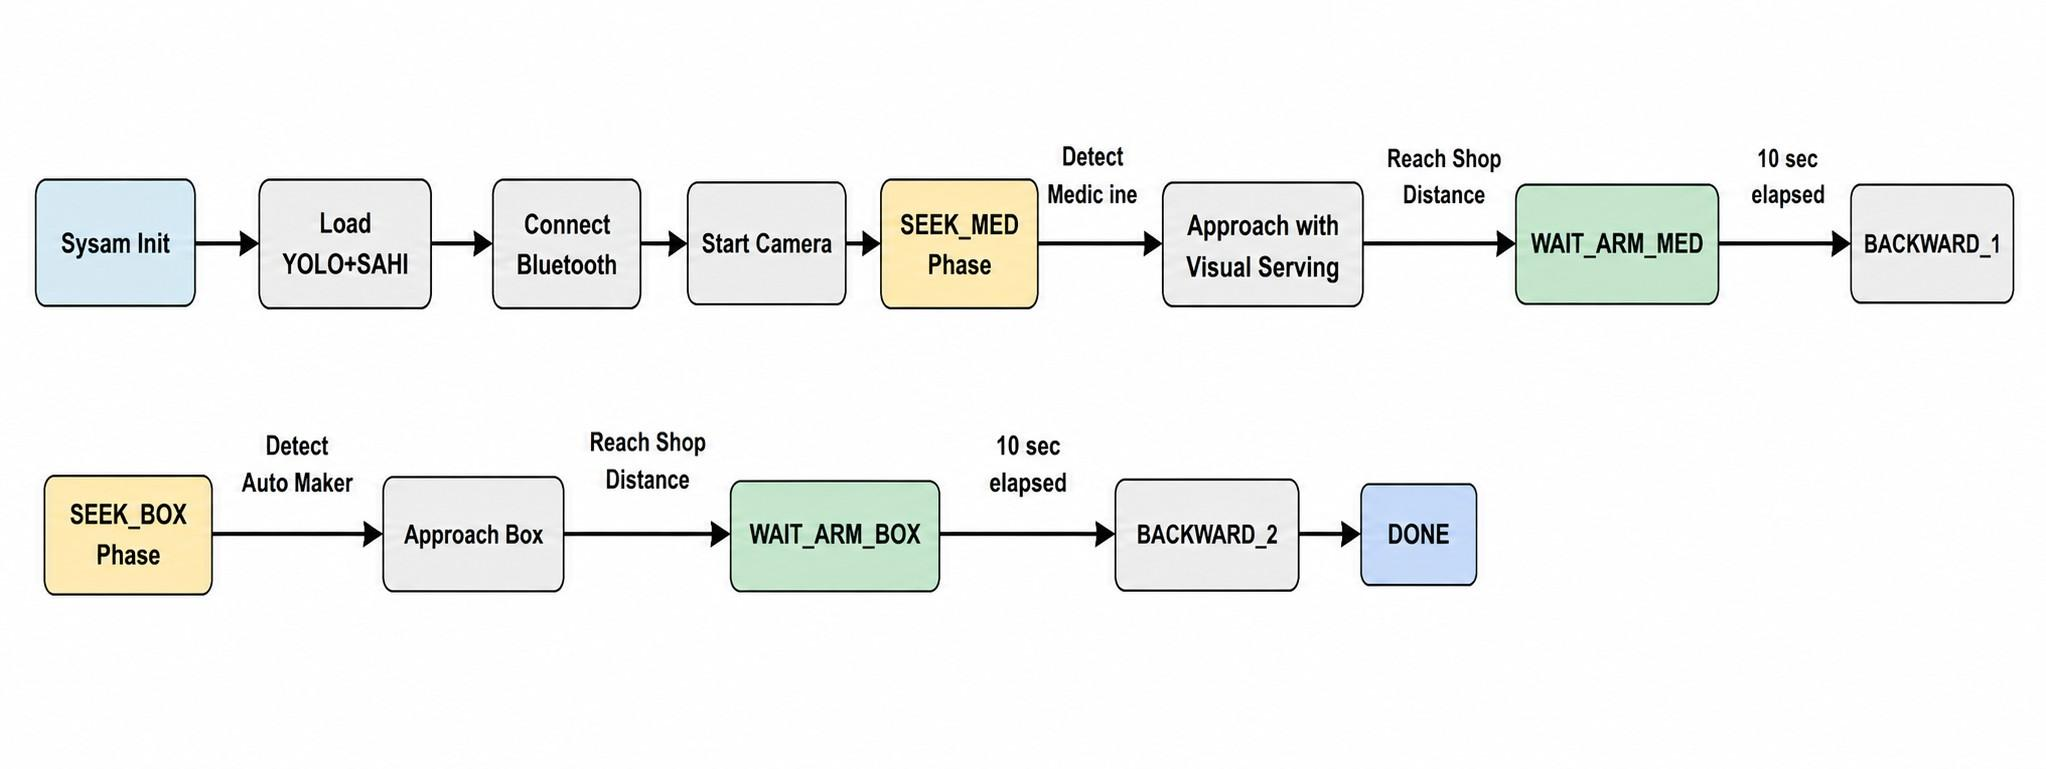
\includegraphics[width=4.47562in,height=1.68219in]{./media/image8.jpg}
\caption{System Architecture diagram showing the execution layer, decision layer, and perception layer for the mobile robot.\label{fig:fig10}}
\end{figure}

\begin{figure}[htbp]
\centering
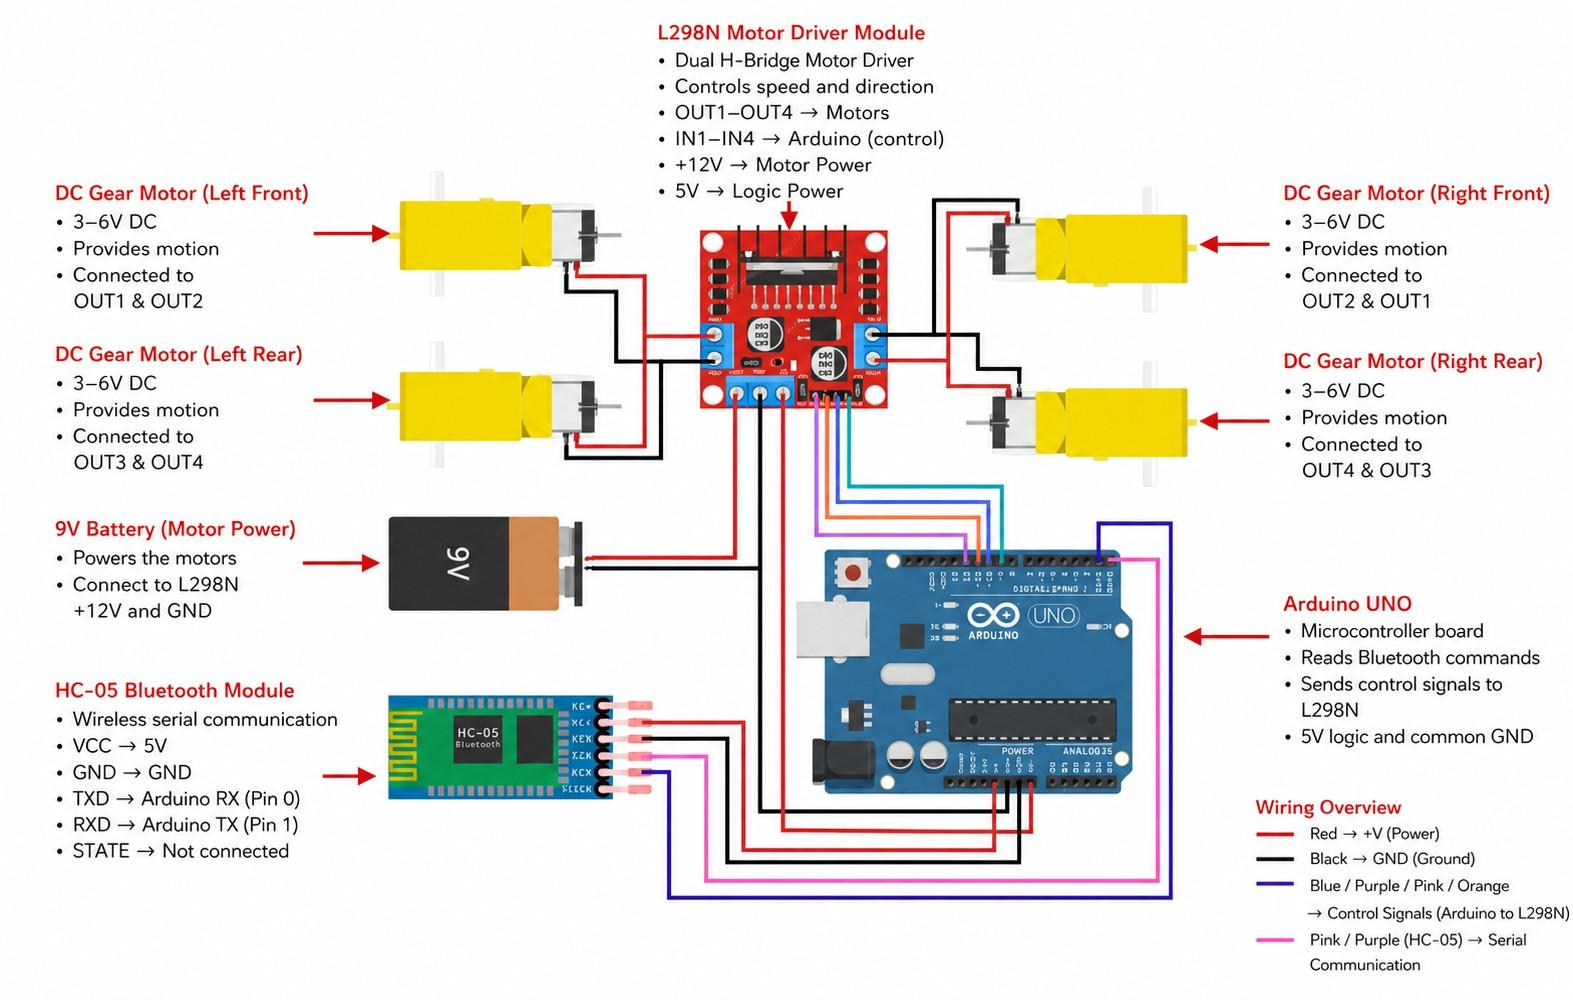
\includegraphics[width=4.42406in,height=2.8125in]{./media/image70.jpg}
\caption{Hardware architecture and communication flow diagram showing the connection between the host PC, Arduino, L298N, HC-05, and motors.\label{fig:fig11}}
\end{figure}

\subsection{Bluetooth Locomotion Control
Protocol}\label{bluetooth-locomotion-control-protocol}

Locomotion commands are transmitted from the host PC to the Arduino Uno
using a lightweight single-character Bluetooth protocol. The host PC
computes visual servoing adjustments and transmits characters over
virtual serial COM ports. The Arduino reads the incoming serial byte and
immediately switches the digital output pins to configure the motor
state as shown in Table~\ref{tab:table10}.

\begin{longtable}[]{@{}
  >{\raggedright\arraybackslash}p{(\linewidth - 4\tabcolsep) * \real{0.1123}}
  >{\raggedright\arraybackslash}p{(\linewidth - 4\tabcolsep) * \real{0.1717}}
  >{\raggedright\arraybackslash}p{(\linewidth - 4\tabcolsep) * \real{0.4005}}@{}}
\caption{Motor Locomotion Command Protocol\label{tab:table10}}\\

\toprule\noalign{}
\begin{minipage}[b]{\linewidth}\centering
\textbf{Command}
\end{minipage} & \begin{minipage}[b]{\linewidth}\centering
\textbf{Locomotion State}
\end{minipage} & \begin{minipage}[b]{\linewidth}\raggedright

\textbf{Motor Pin Configurations}

\end{minipage} \\
\begin{minipage}[b]{\linewidth}\centering
'F'
\end{minipage} & \begin{minipage}[b]{\linewidth}\centering
Move Forward
\end{minipage} & \begin{minipage}[b]{\linewidth}\raggedright

IN1=HIGH, IN2=LOW, IN3=LOW, IN4=HIGH

\end{minipage} \\
\begin{minipage}[b]{\linewidth}\centering
'B'
\end{minipage} & \begin{minipage}[b]{\linewidth}\centering
Move Backward
\end{minipage} & \begin{minipage}[b]{\linewidth}\raggedright

IN1=LOW, IN2=HIGH, IN3=HIGH, IN4=LOW

\end{minipage} \\
\begin{minipage}[b]{\linewidth}\centering
'R'
\end{minipage} & \begin{minipage}[b]{\linewidth}\centering
Turn Right
\end{minipage} & \begin{minipage}[b]{\linewidth}\raggedright

IN1=HIGH, IN2=LOW, IN3=HIGH, IN4=LOW

\end{minipage} \\
\begin{minipage}[b]{\linewidth}\centering
'L'
\end{minipage} & \begin{minipage}[b]{\linewidth}\centering
Turn Left
\end{minipage} & \begin{minipage}[b]{\linewidth}\raggedright

IN1=LOW, IN2=HIGH, IN3=LOW, IN4=HIGH

\end{minipage} \\
\begin{minipage}[b]{\linewidth}\centering
'S'
\end{minipage} & \begin{minipage}[b]{\linewidth}\centering
Stop Locomotion
\end{minipage} & \begin{minipage}[b]{\linewidth}\raggedright

IN1=LOW, IN2=LOW, IN3=LOW, IN4=LOW

\end{minipage} \\
\midrule\noalign{}
\endhead
\bottomrule\noalign{}
\endlastfoot
\end{longtable}

\subsection{Dataset Preparation, Augmentation, and Transfer
Learning}\label{dataset-preparation-augmentation-and-transfer-learning}

To train the YOLO object detection model, a custom dataset of local
medicine packages (Milga, Antopral, and Staturic) was collected using
the Roboflow platform. The initial dataset contained 150 raw images. Due
to the small dataset size, the model was highly susceptible to
overfitting and poor generalization. To mitigate this, Roboflow was
configured to generate

3 augmented samples per image using rotation
(\emph{$\pm$}15$^\circ$), horizontal shear
(\emph{$\pm$}10$^\circ$), and vertical shear
(\emph{$\pm$}10$^\circ$). This expanded the dataset to 327
images, split into 297 training images and 30 validation images.

\begin{longtable}[]{@{}
  >{\raggedright\arraybackslash}p{(\linewidth - 6\tabcolsep) * \real{0.0969}}
  >{\raggedright\arraybackslash}p{(\linewidth - 6\tabcolsep) * \real{0.1237}}
  >{\raggedright\arraybackslash}p{(\linewidth - 6\tabcolsep) * \real{0.0846}}
  >{\raggedright\arraybackslash}p{(\linewidth - 6\tabcolsep) * \real{0.3287}}@{}}
\caption{Initial Dataset Class Distribution\label{tab:table11}}\\

\toprule\noalign{}
\begin{minipage}[b]{\linewidth}\centering
\textbf{Class ID}
\end{minipage} & \begin{minipage}[b]{\linewidth}\raggedright

\textbf{Class Name}

\end{minipage} & \begin{minipage}[b]{\linewidth}\centering
\textbf{Images}
\end{minipage} & \begin{minipage}[b]{\linewidth}\raggedright

\textbf{Description}

\end{minipage} \\
\begin{minipage}[b]{\linewidth}\centering
0
\end{minipage} & \begin{minipage}[b]{\linewidth}\raggedright

Milga

\end{minipage} & \begin{minipage}[b]{\linewidth}\centering
50
\end{minipage} & \begin{minipage}[b]{\linewidth}\raggedright

Primary target for pick-and-place trials

\end{minipage} \\
\begin{minipage}[b]{\linewidth}\centering
1
\end{minipage} & \begin{minipage}[b]{\linewidth}\raggedright

Antopral

\end{minipage} & \begin{minipage}[b]{\linewidth}\centering
50
\end{minipage} & \begin{minipage}[b]{\linewidth}\raggedright

Secondary class (distractor)

\end{minipage} \\
\begin{minipage}[b]{\linewidth}\centering
2
\end{minipage} & \begin{minipage}[b]{\linewidth}\raggedright

Staturic

\end{minipage} & \begin{minipage}[b]{\linewidth}\centering
50
\end{minipage} & \begin{minipage}[b]{\linewidth}\raggedright

Tertiary class (distractor)

\end{minipage} \\
\midrule\noalign{}
\endhead
\bottomrule\noalign{}
\endlastfoot
\end{longtable}

\begin{longtable}[]{@{}
  >{\raggedright\arraybackslash}p{(\linewidth - 4\tabcolsep) * \real{0.2333}}
  >{\raggedright\arraybackslash}p{(\linewidth - 4\tabcolsep) * \real{0.1304}}
  >{\raggedright\arraybackslash}p{(\linewidth - 4\tabcolsep) * \real{0.4290}}@{}}
\caption{Dataset Augmentation Parameters\label{tab:table12}}\\

\toprule\noalign{}
\begin{minipage}[b]{\linewidth}\raggedright

\textbf{Augmentation Technique}

\end{minipage} & \begin{minipage}[b]{\linewidth}\raggedright

\textbf{Value Range}

\end{minipage} & \begin{minipage}[b]{\linewidth}\raggedright

\textbf{Design Rationale}

\end{minipage} \\
\begin{minipage}[b]{\linewidth}\raggedright

Rotation

\end{minipage} & \begin{minipage}[b]{\linewidth}\raggedright

\emph{$\pm$}15\emph{$^\circ$}

\end{minipage} & \begin{minipage}[b]{\linewidth}\raggedright

Simulates rotation variations of packages on floor

\end{minipage} \\
\begin{minipage}[b]{\linewidth}\raggedright

Horizontal Shear

\end{minipage} & \begin{minipage}[b]{\linewidth}\raggedright

\emph{$\pm$}10\emph{$^\circ$}

\end{minipage} & \begin{minipage}[b]{\linewidth}\raggedright

Simulates camera pitch and skew angles

\end{minipage} \\
\begin{minipage}[b]{\linewidth}\raggedright

Vertical Shear

\end{minipage} & \begin{minipage}[b]{\linewidth}\raggedright

\emph{$\pm$}10\emph{$^\circ$}

\end{minipage} & \begin{minipage}[b]{\linewidth}\raggedright

Simulates non-orthogonal viewing perspectives

\end{minipage} \\
\begin{minipage}[b]{\linewidth}\raggedright

Multiplication Factor

\end{minipage} & \begin{minipage}[b]{\linewidth}\raggedright

3x

\end{minipage} & \begin{minipage}[b]{\linewidth}\raggedright

Generates 3 unique augmented variations per image

\end{minipage} \\
\midrule\noalign{}
\endhead
\bottomrule\noalign{}
\endlastfoot
\end{longtable}

\begin{figure}[htbp]
\centering
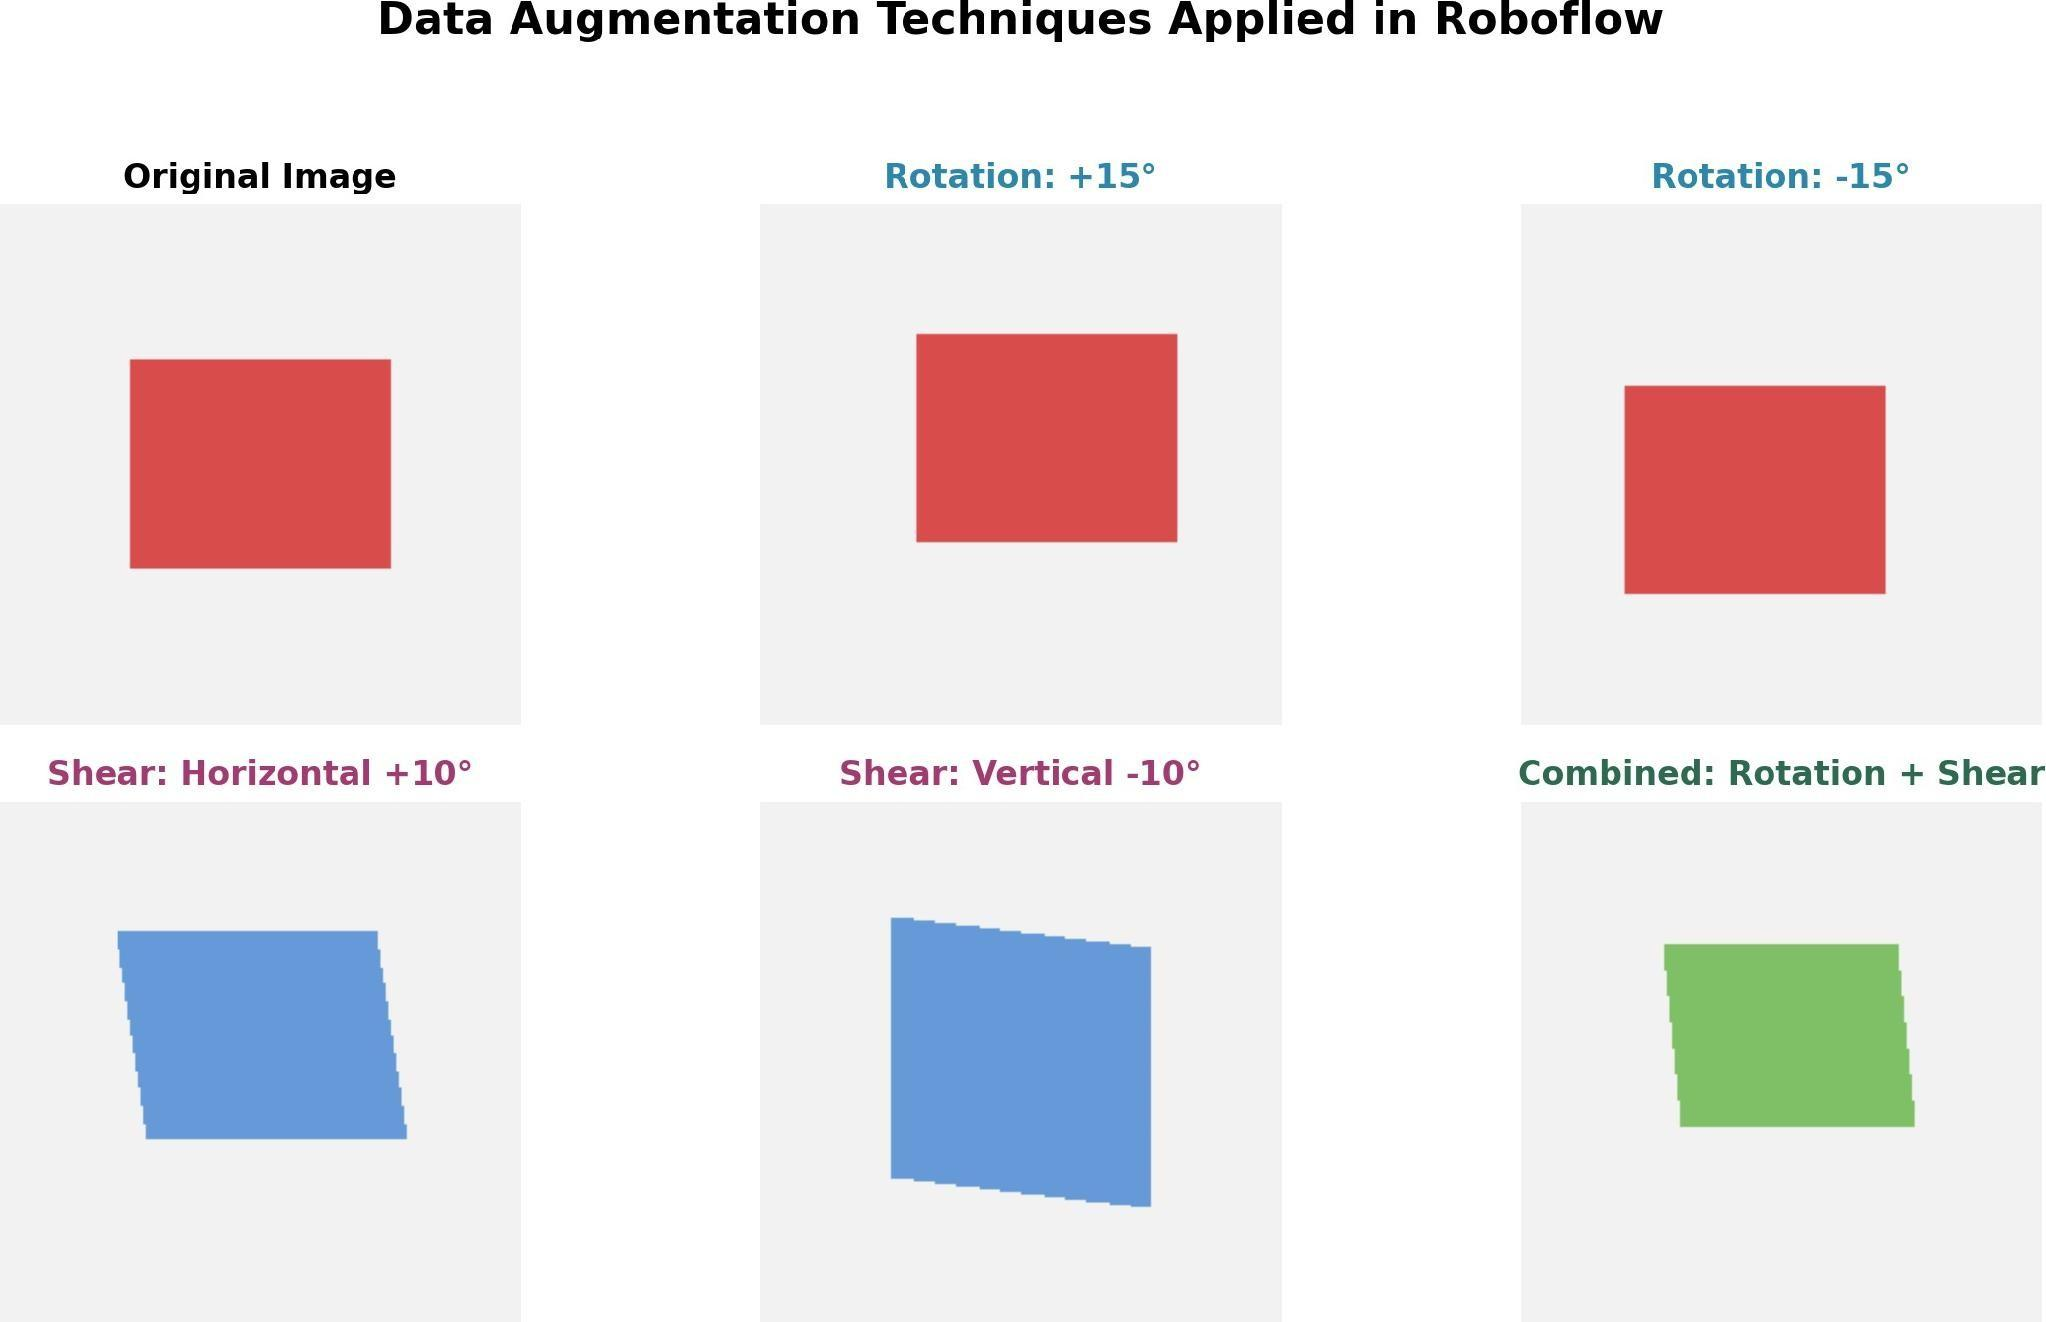
\includegraphics[width=5.32812in,height=3.44271in]{./media/image79.jpg}
\caption{Examples of dataset augmentation: original image, rotation, horizontal/vertical shear, and combined transformations.\label{fig:fig12}}
\end{figure}

To maximize detection performance, we applied transfer learning from the
pre-trained COCO dataset checkpoint (yolov8n.pt). Crucially, we froze
the first 10 layers of the YOLO backbone (freeze=10) during training.
This prevented the model from modifying the low-level visual feature
extractors (lines, edges, textures) already learned from COCO,
fine-tuning only the higher-level detection head on our medicine
dataset, thus protecting the model from catastrophic forgetting. The
overall training configuration is summarized in Table~\ref{tab:table13}.

\begin{table}[htbp]
\centering
\caption{Mobile YOLO Training Configuration\label{tab:table13}}
\begin{tabular}{ll}
\toprule
\textbf{Parameter} & \textbf{Configuration Value} \\
\midrule
Pre-trained Model Base & yolov8n.pt (COCO dataset) \\
Backbone Freezing Layer & freeze=10 (layers 1--10 frozen) \\
Optimizer & AdamW (learning rate = 0.001) \\
Batch Size & 16 \\
Training Epochs & 120 (with early stopping patience = 30) \\
Input Resolution & $640 \times 640$ pixels \\
Augmented Dataset Size & 327 images (297 train, 30 validation) \\
\bottomrule
\end{tabular}
\end{table}

\subsection{YOLOv8-SAHI Perception and ArUco
Detection}\label{yolov8-sahi-perception-and-aruco-detection}

During autonomous navigation, the perception pipeline runs YOLOv8n
enhanced by Slicing Aided Hyper Inference (SAHI). SAHI splits the 640
\emph{$\times$} 360 camera frame into overlapping 320 \emph{$\times$} 320 pixel
slices, runs inference on each slice, and merges bounding boxes using
Non-Maximum Suppression (NMS). This addresses the small-object detection
issue when the robot is far from the medicine box. For the drop-off phase, the robot utilizes OpenCV's dedicated ArUco marker detection module. ArUco markers serve as robust visual landmarks for identifying the drop-off box location. Unlike natural features that can be ambiguous, ArUco markers provide a unique, easily detectable binary pattern that can be identified regardless of lighting conditions, viewing angle, or partial occlusion. The system uses the ArUco \texttt{DICT\_4X4\_50} dictionary, which provides 50 unique marker IDs, each represented by a 4\emph{$\times$}4 binary grid pattern surrounded by a black border for localization.

\subsubsection{Detection Implementation}\label{detection-implementation}

The ArUco marker detection is implemented in a separate Python module called \texttt{box\_maker.py}, which provides the \texttt{check\_box\_marker()} function. This function takes a camera frame, the ArUco detector object, and the target box ID as inputs. The function converts the input frame to grayscale to maximize edge contrast, runs the ArUco detector to find all markers in the frame, and checks if any detected marker matches the target box ID (ID 0). When a matching marker is found, the function calculates the bounding box coordinates ($x_1, y_1, x_2, y_2$), the center X position, and the average size of the marker from its corner coordinates. These geometric measurements are used by the state machine to navigate the robot toward the box and determine when the robot has reached the correct position for depositing the medicine.

\subsubsection{Marker Geometry Calculations}\label{marker-geometry-calculations}

The geometric calculations performed on the detected ArUco marker are essential for accurate robot navigation. The four corner points of each detected marker are extracted from the OpenCV detector output. The bounding box is computed as the minimum and maximum X and Y coordinates across all four corners:
\begin{align}
x_1 &= \min(x_{c1}, x_{c2}, x_{c3}, x_{c4}) \\
x_2 &= \max(x_{c1}, x_{c2}, x_{c3}, x_{c4}) \\
y_1 &= \min(y_{c1}, y_{c2}, y_{c3}, y_{c4}) \\
y_2 &= \max(y_{c1}, y_{c2}, y_{c3}, y_{c4})
\end{align}
The center X coordinate is calculated as the average of the left and right edges:
\begin{equation}
x_{center} = \frac{x_1 + x_2}{2}
\end{equation}
This center X coordinate is used to determine the angular error between the robot heading and the box direction. The marker size is computed as the average of the bounding box width and height:
\begin{equation}
S_{marker} = \frac{(x_2 - x_1) + (y_2 - y_1)}{2}
\end{equation}
The marker size $S_{marker}$ serves as a proxy for distance estimation since larger markers indicate the robot is closer to the box. This size-based distance estimation triggers the stop condition when the size exceeds the predefined \texttt{STOP\_DISTANCE\_BOX} threshold of 180 pixels.

\begin{table}[htbp]
\centering
\caption{SAHI Inference Configuration Parameters\label{tab:table14}}
\begin{tabular}{ll}
\toprule
\textbf{SAHI Parameter} & \textbf{Configuration Value} \\
\midrule
Slice Height & 320 pixels \\
Slice Width & 320 pixels \\
Overlap Height Ratio & 0.2 \\
Overlap Width Ratio & 0.2 \\
Confidence Threshold & 0.78 \\
Inference Device & CUDA GPU (cuda:0) \\
\bottomrule
\end{tabular}
\end{table}

\begin{figure}[htbp]
\centering
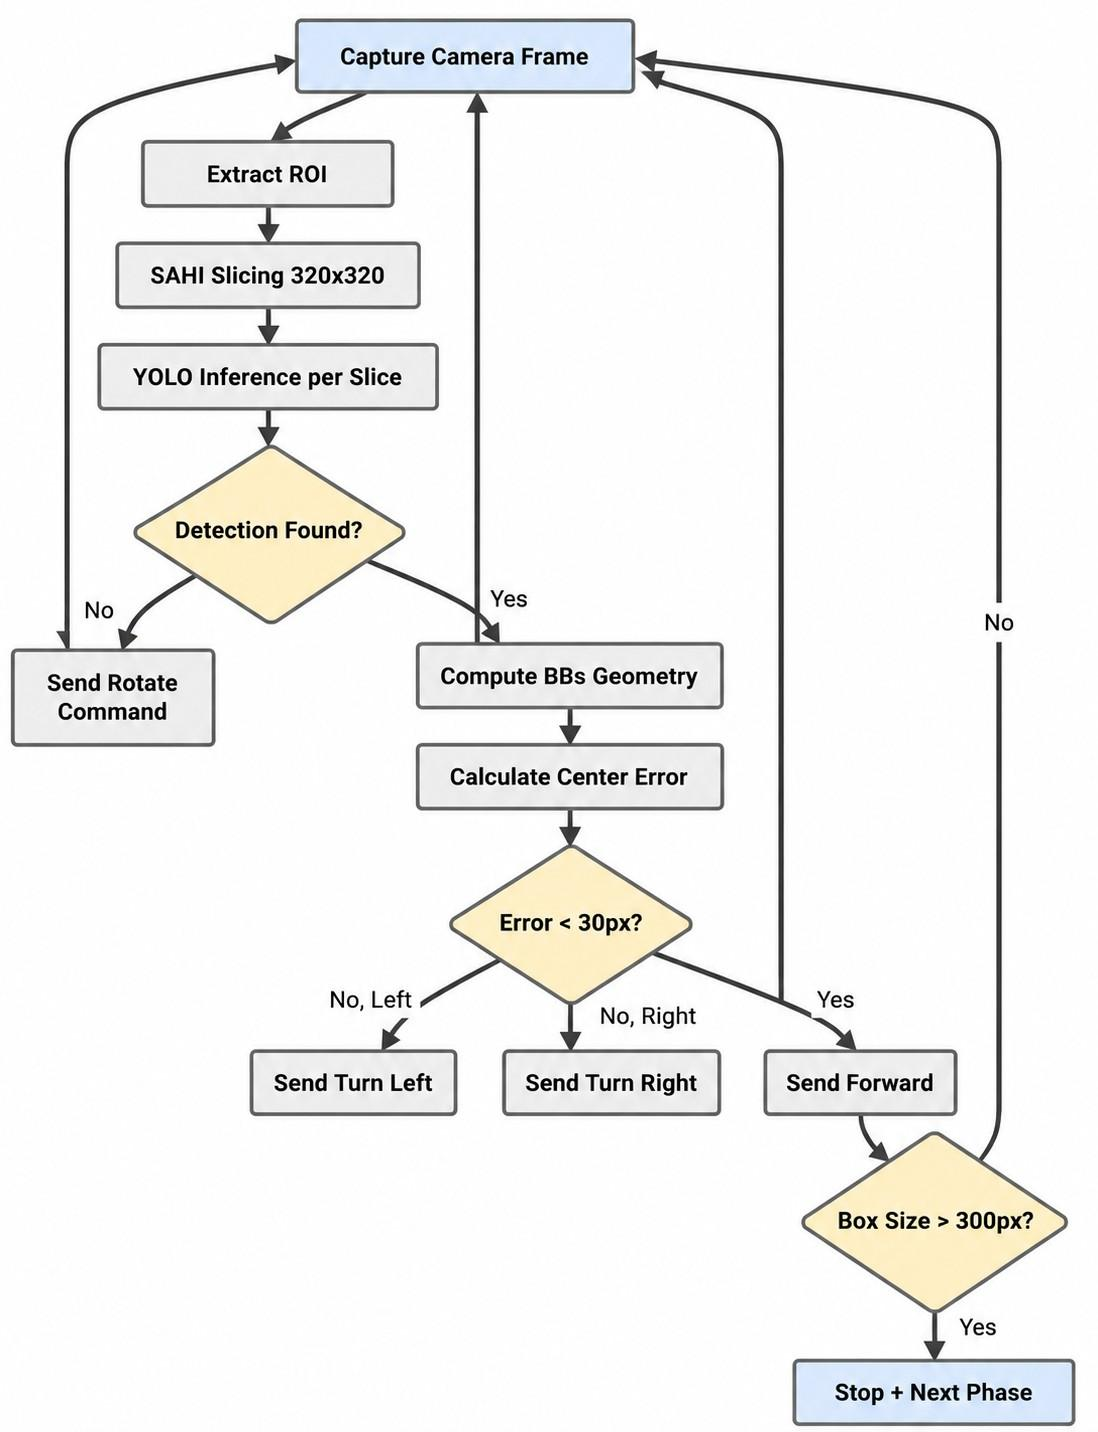
\includegraphics[width=3.43125in,height=4.475in]{./media/image85.jpg}
\caption{YOLOv8-SAHI perception and visual servoing control flowchart.\label{fig:fig14}}
\end{figure}

\begin{figure}[htbp]
\centering
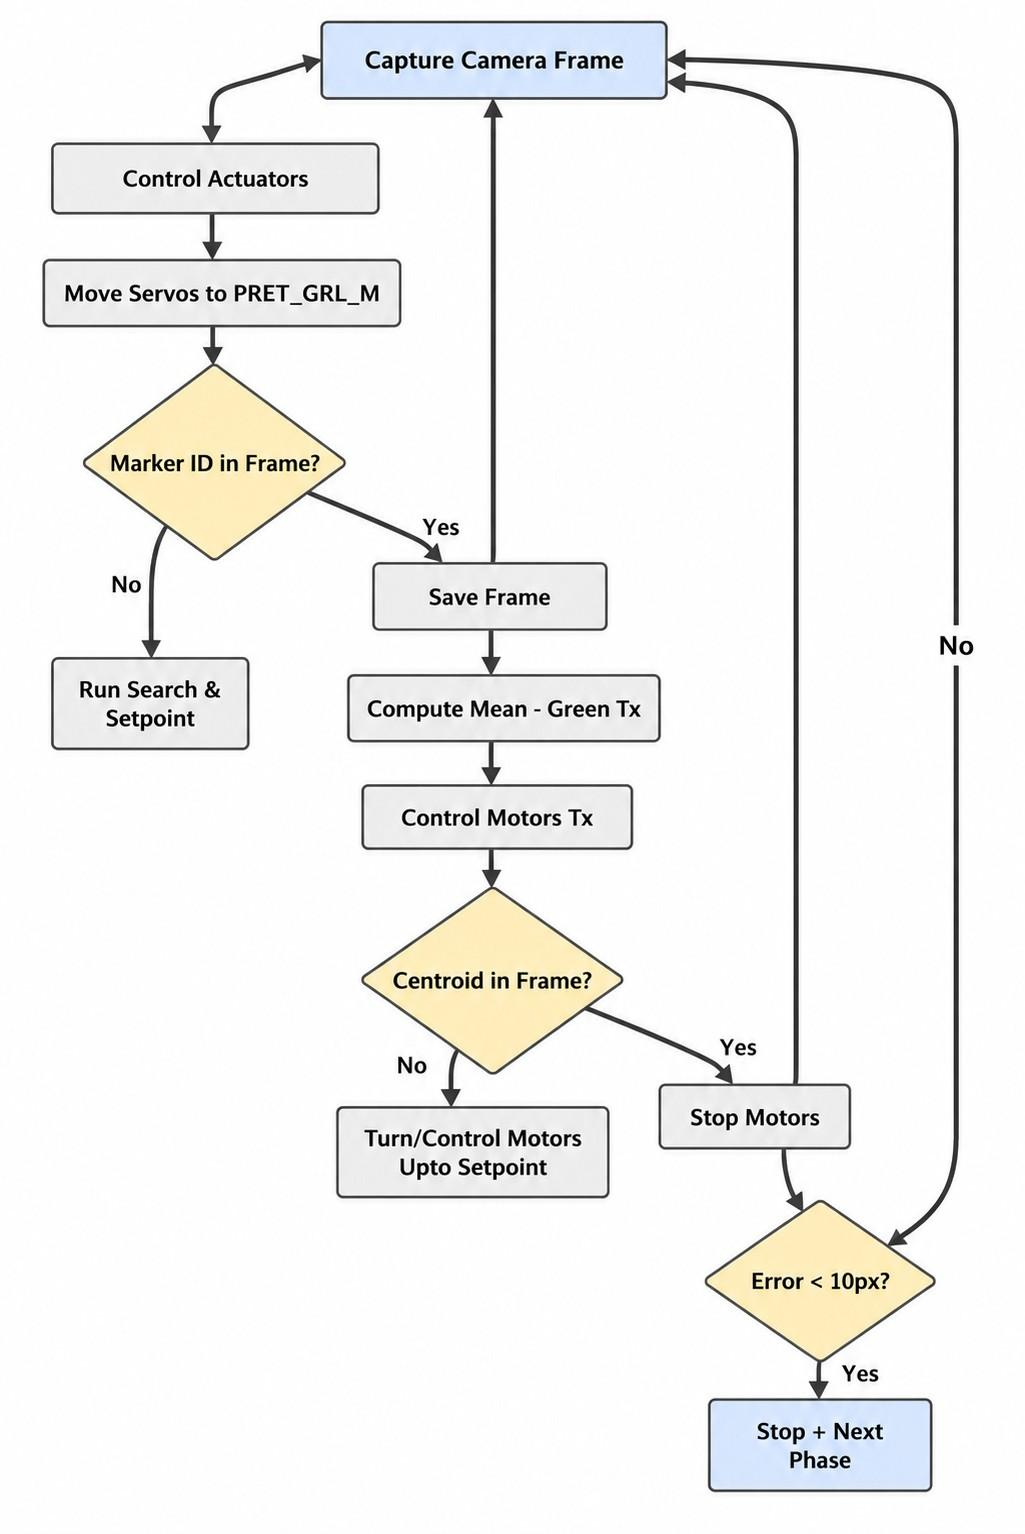
\includegraphics[width=3.41667in,height=5.11333in]{./media/image59.jpg}
\caption{ArUco marker detection and visual servoing docking flowchart.\label{fig:fig15}}
\end{figure}

\subsection{Finite State Machine and Control Loop}
\label{finite-state-machine-and-control-loop}

The navigation and manipulation workflow is orchestrated by an 8-phase Finite State Machine (FSM). Visual servoing adjusts the robot steering by computing the error between the detected bounding box center $X_{\text{bbox}}$ and the frame center $X_{\text{center}}$ ($320$ pixels). The alignment error $e$ is defined as:
\begin{equation}
e = X_{\text{bbox}} - X_{\text{center}}
\end{equation}

If $|e| > \theta_{\text{align}}$ (where the alignment threshold $\theta_{\text{align}} = 80$ pixels), the robot sends turn commands (`'L'` or `'R'`) to align with the target. Once aligned, the robot moves forward (`'F'`). 

The robot stops locomotion (`'S'`) and transitions states when the bounding box average size exceeds the stop distance threshold ($200$ pixels for medicine, $180$ pixels for the drop-off box). The FSM phase sequence and control parameters are detailed in Table~\ref{tab:table15} and Table~\ref{tab:table16}.

\begin{table}[htbp]
\centering
\caption{Mobile Robot Finite State Machine (FSM) Phases}
\label{tab:table15}
\begin{tabular}{c l p{8.5cm}}
\toprule
\textbf{Phase ID} & \textbf{State Name} & \textbf{Description} \\
\midrule
0 & SEEK\_MED      & Search environment and approach target medicine box. \\
1 & WAIT\_ARM\_MED  & Pause locomotion, trigger robotic arm grasp (10 seconds). \\
2 & BACKWARD\_1    & Execute pulsed backward motion away from shelf (1.5 seconds). \\
3 & SEEK\_BOX      & Rotate to search for ArUco marker ID 0. \\
4 & APPROACH\_BOX  & Navigate and align with drop-off box using visual servoing. \\
5 & WAIT\_ARM\_BOX  & Trigger robotic arm deposit sequence (10 seconds). \\
6 & BACKWARD\_2    & Move backward away from box (1.5 seconds). \\
7 & DONE           & Stop operation, display completion state. \\
\bottomrule
\end{tabular}
\end{table}

\begin{table}[htbp]
\centering
\caption{Visual Servoing Control Loop Parameters\label{tab:table16}}
\begin{tabular}{ll}
\toprule
\textbf{Parameter} & \textbf{Operational Value} \\
\midrule
Frame Center ($X_{center}$) & 320 pixels \\
Alignment Zone ($\theta_{align}$) & $\pm 80$ pixels \\
Stop Threshold (Medicine) & 200 pixels (average bounding box size) \\
Stop Threshold (Box) & 180 pixels (average bounding box size) \\
Arm Gantry Grab Delay & 10 seconds \\
Pulsed Backward Duration & 1.5 seconds (0.12s pulse on, 0.1s off) \\
Search Sweep Timeout & 2.0 seconds per rotation step \\
\bottomrule
\end{tabular}
\end{table}

\subsection{Main Control Script and Parameter Configuration}\label{main-control-script-and-parameter-configuration}

The main Python control script serves as the central coordinator of the mobile robot subsystem. It initializes all subsystems including the Bluetooth connection, the YOLO model with its SAHI wrapper, the ArUco detector, and the camera feed, then enters a continuous processing loop. In each iteration of the loop, the script captures a camera frame, extracts the Region of Interest (ROI), runs SAHI-based object detection on the ROI, evaluates the state machine logic, computes the appropriate motor command, and sends it to the Arduino via Bluetooth. The ROI is defined as a rectangular sub-region of the frame (from coordinates (120, 60) to (520, 330)), which focuses the detection on the central area of the camera view where targets are expected to appear.

The key configuration parameters for the main control script are summarized in Table~\ref{tab:table_main_script_params}.

\begin{table}[htbp]
\centering
\caption{Main Script Configuration Parameters\label{tab:table_main_script_params}}
\begin{tabular}{lll}
\toprule
\textbf{Parameter} & \textbf{Value} & \textbf{Purpose} \\
\midrule
\texttt{MODEL\_PATH} & \texttt{D:/best (3).pt} & Path to trained YOLO model weights \\
\texttt{TARGET\_MEDICINE} & \texttt{Milga} & Target class for pick operation \\
\texttt{CONF\_THRESHOLD} & 0.78 & Minimum detection confidence score \\
\texttt{COM\_PORT} & \texttt{COM7} & Bluetooth serial port \\
\texttt{BAUD\_RATE} & 9600 & Serial communication speed \\
\texttt{ROI Coordinates} & (120,60)-(520,330) & Detection region of interest \\
\bottomrule
\end{tabular}
\end{table}

\chapter{IMPLEMENTATION \& RESULTS}
\label{implementation-results}

\section{Software Code Implementation}
\label{software-code-implementation}

The system implementation consists of core code blocks across the robotic hand, backend, and frontend.

\subsection{MediaPipe Landmark Mimicry and Filter}
\label{mediapipe-landmark-mimicry-and-filter}

The MediaPipe tracker module \texttt{hand\_memic.py} runs a continuous video frame processing loop. The landmarks are processed to compute normalized finger extension ratios, which are mapped to servo angles.

These raw ratios are converted to servo command angles using per-finger linear interpolation ranges:
\begin{equation}
A_i = \text{clamp}\left( \frac{R_i - R_{i,\min}}{R_{i,\max} - R_{i,\min}} \times 100 + 50, \, 50, \, 150 \right)
\end{equation}

\subsection{Distance Filtering and Stability
Control}\label{distance-filtering-and-stability-control}

The distance reading obtained from the HC-SR04 palm sensor is noisy. We
implement the DistanceFilter
class:
\begin{figure}[htbp]
\centering
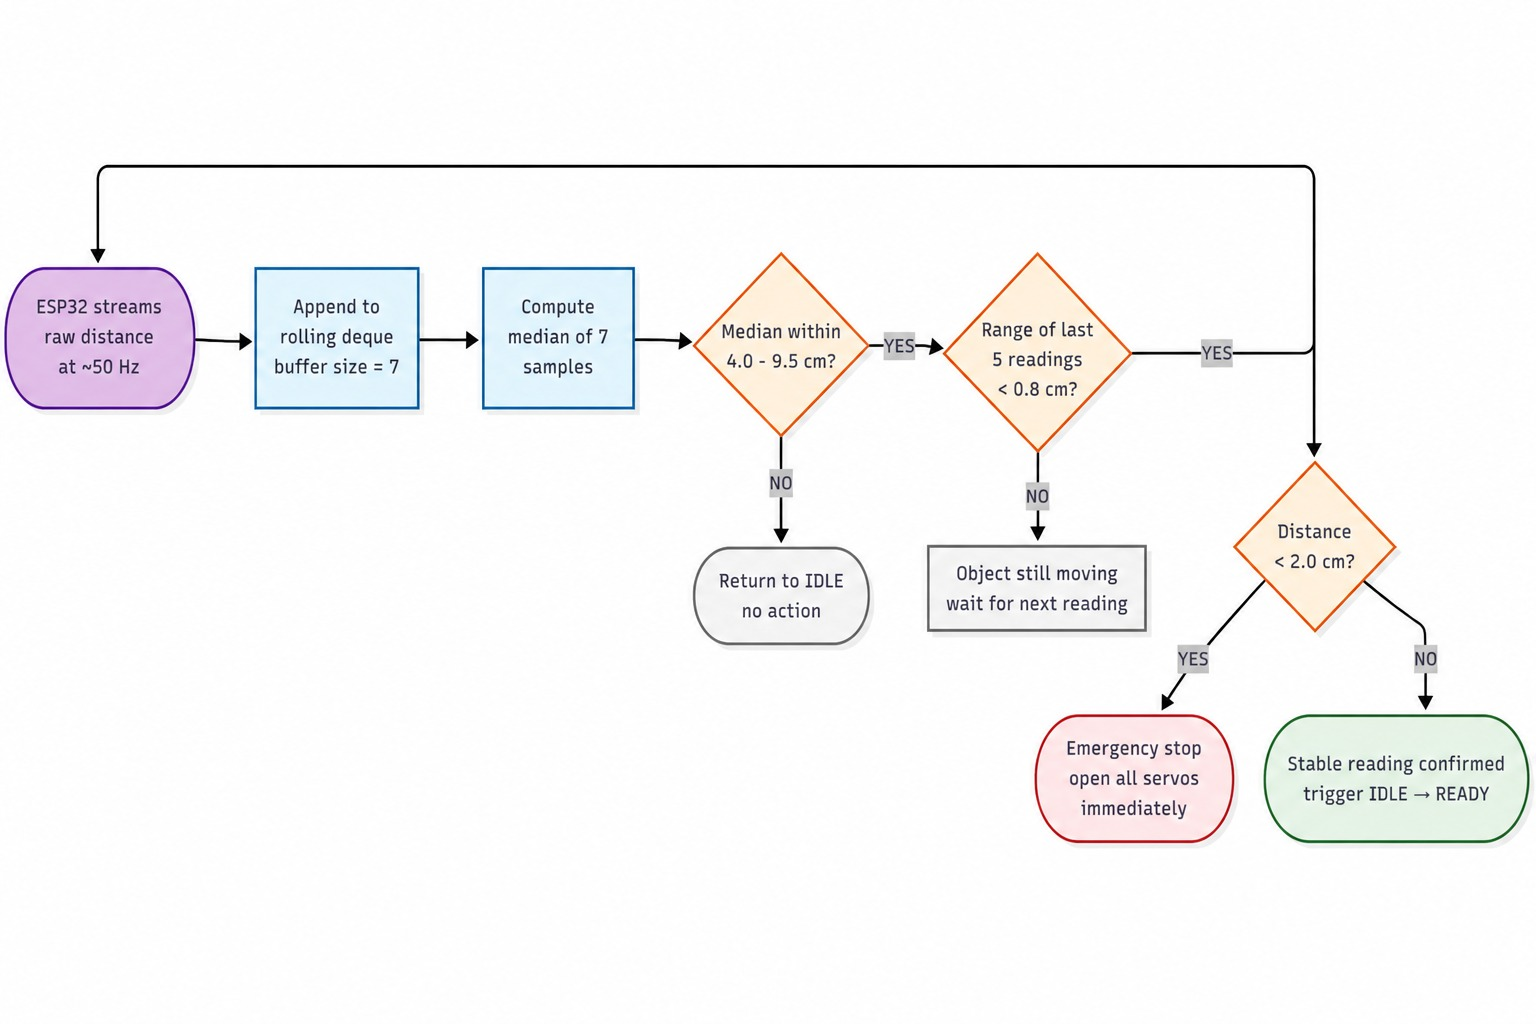
\includegraphics[width=5.36736in,height=3.16181in]{./media/joe-fig1.jpeg}
\caption{Distance Filter Class\label{fig:joe-fig1}}
\end{figure}
% \begin{figure}[htbp]
% \centering
% % 
\includegraphics[width=3.675in,height=\textheight,keepaspectratio]{./media/image49.png}
% 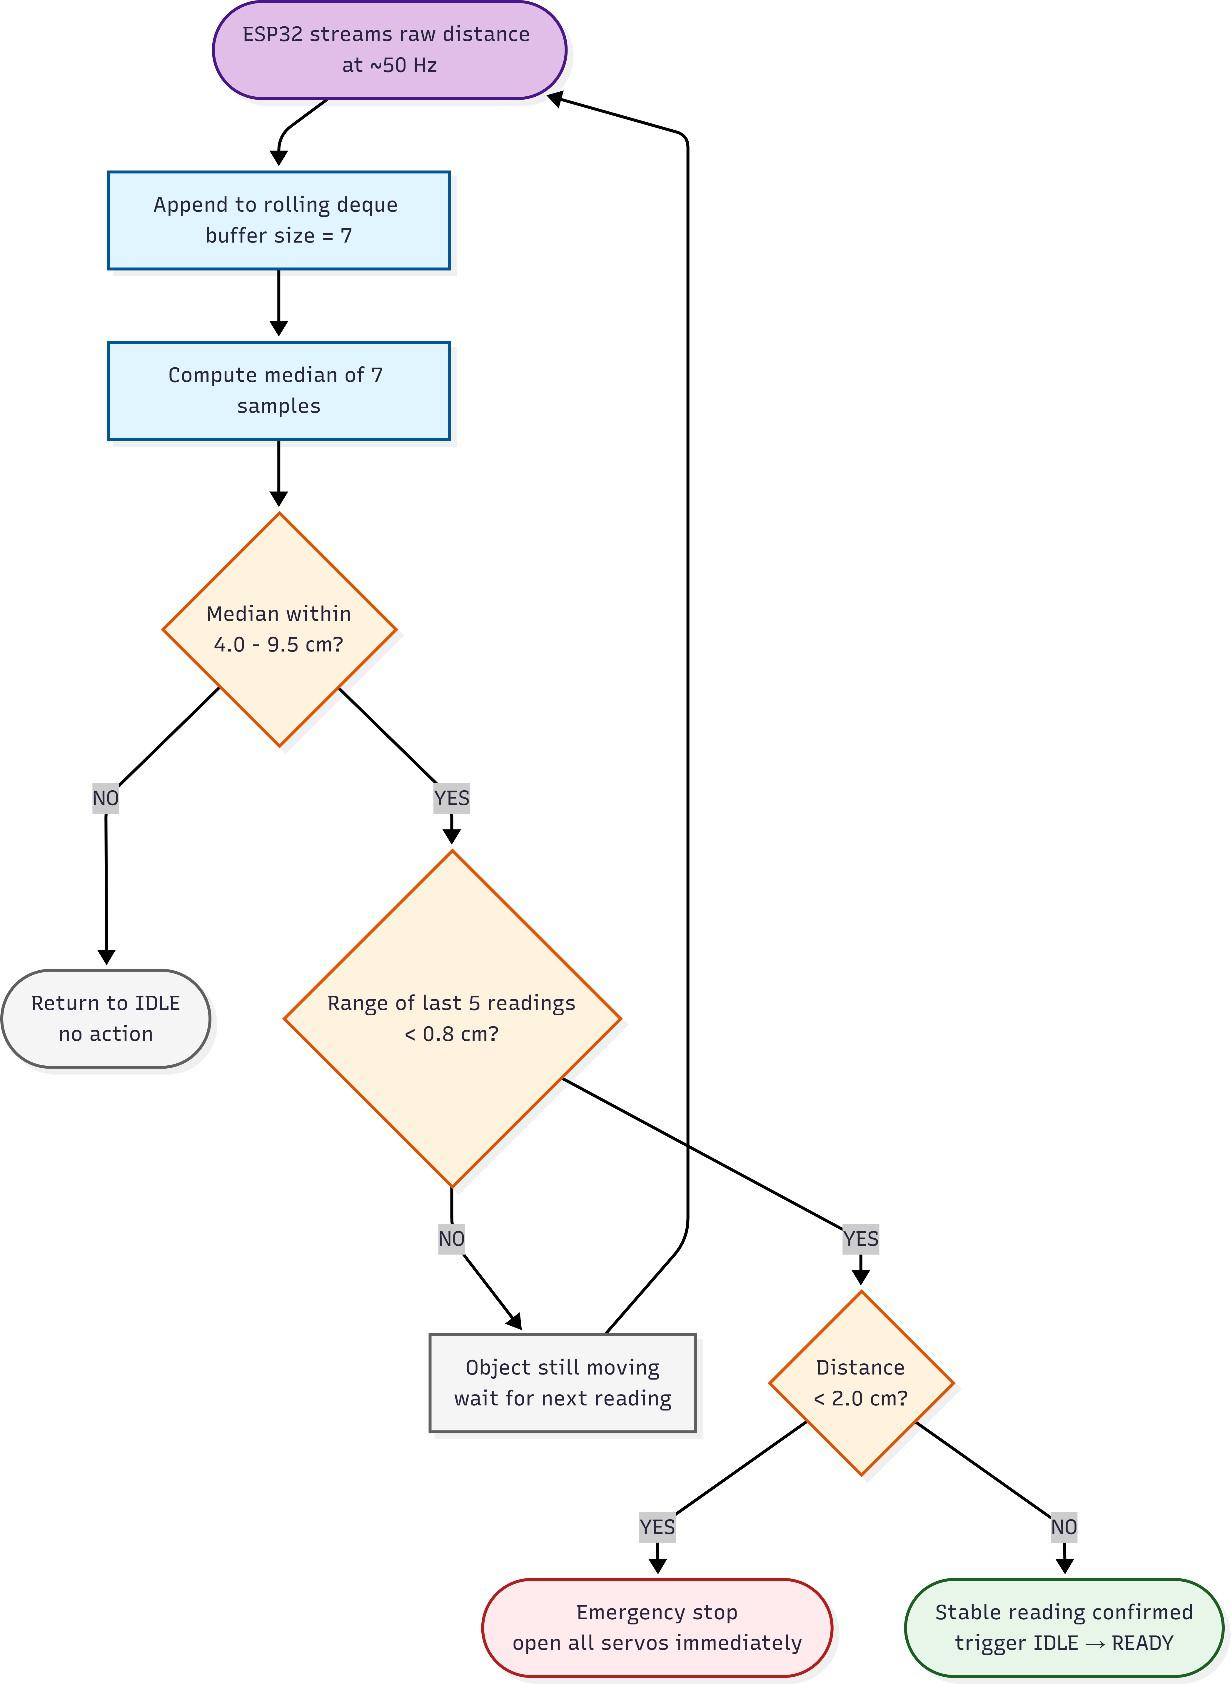
\includegraphics[width=5.00094in,height=6.84125in]{./media/image61.jpg}
% \caption{Signal Flow: Circular Median Filter and Stability Verification Pipeline\label{fig:fig16}}
% \end{figure}

\subsection{Autonomous Finite State Machine}
\label{autonomous-finite-state-machine}

The autonomous controller runs an active loop running at 50 Hz. The state transitions are managed via the \texttt{AutoState} enumeration:

\begin{figure}[htbp]
\centering
% Note: Adjust the image path and dimensions as required for your local project setup
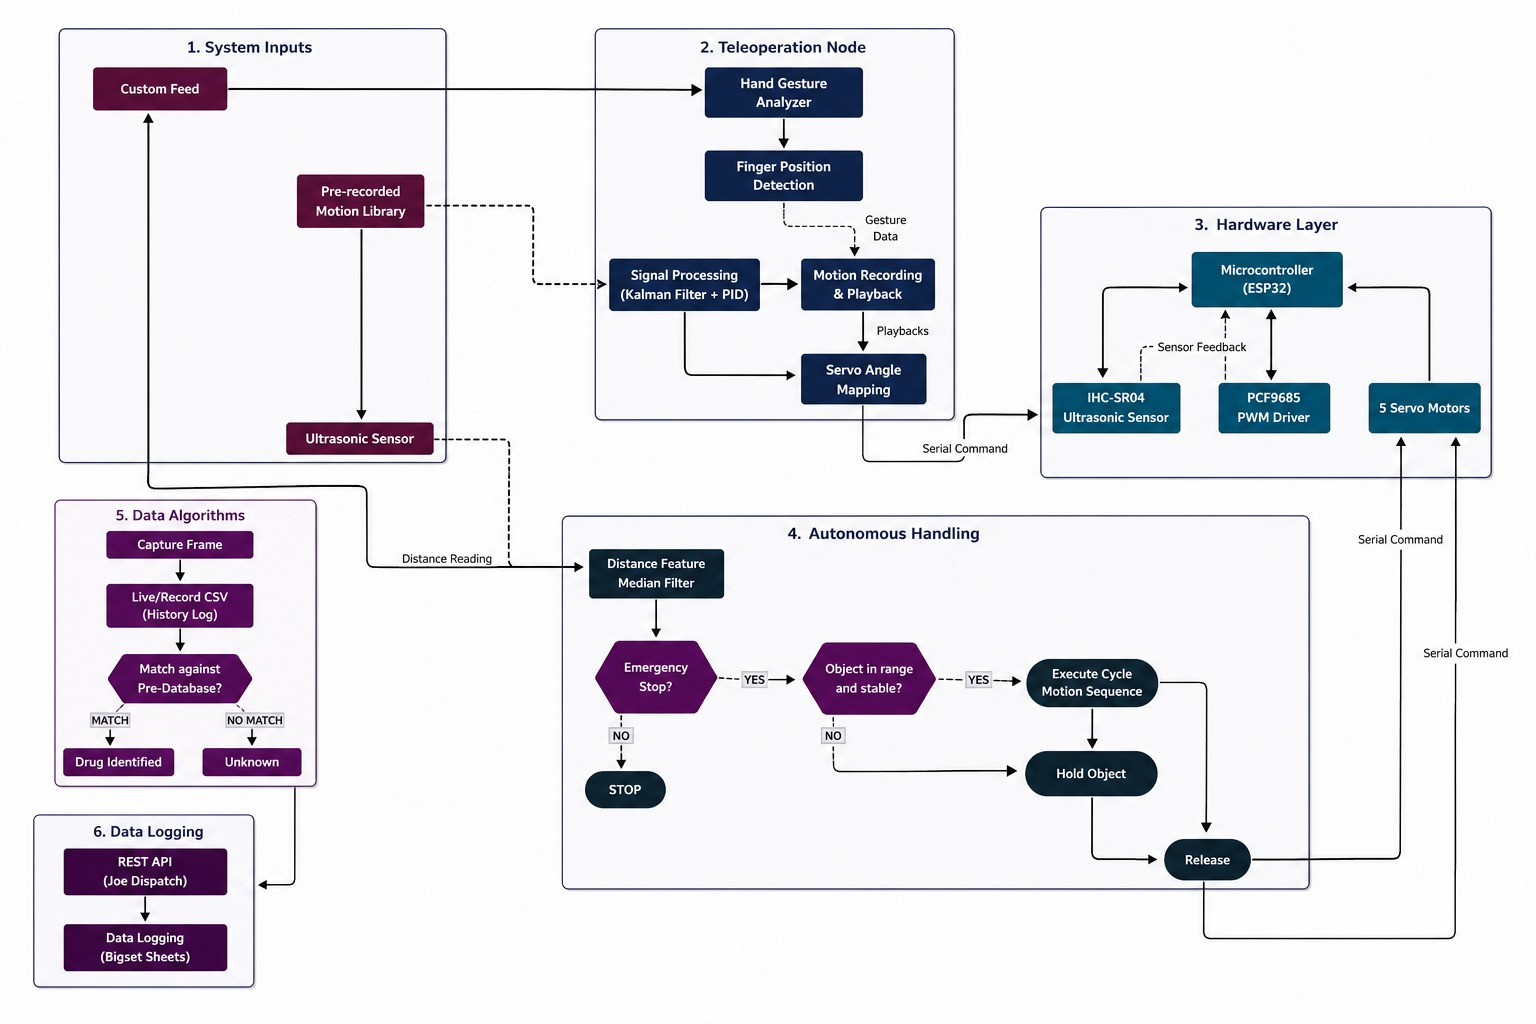
\includegraphics[width=4.92in, height=8.87in, keepaspectratio]{./media/joe-fig2.jpeg}
\caption{State Machine Pipeline: Ultrasonic Detection to Final Robotic Grasp Action}
\label{fig:fig17}
\end{figure}

\begin{itemize}
    \item \textbf{READY:} The sensor detects an object at a stable distance (e.g., 6.5~cm). The system queries the Motion Library to retrieve the matching trajectory.
    \item \textbf{GRABBING:} Executes time-based playback of the trajectory, writing servo command bytes \texttt{"Aa1,a2,a3,a4,a5\textbackslash n"} to the serial port.
    \item \textbf{HOLDING:} The hand holds the object. A separate daemon thread triggers OCR processing to identify the label.
    \item \textbf{RELEASING:} Once the OCR resolves and backend dispatch signals completion, the hand opens all fingers and releases the package, pausing 2~seconds before re-entering detection.
\end{itemize}

\subsection{Asynchronous OCR Concurrency
Timeline}\label{asynchronous-ocr-concurrency-timeline}

OCR execution takes 1.8 seconds on average. If performed in the main
control loop, it would cause the state machine to freeze. We offload the
execution to a daemon thread:

\begin{figure}[htbp]
\centering
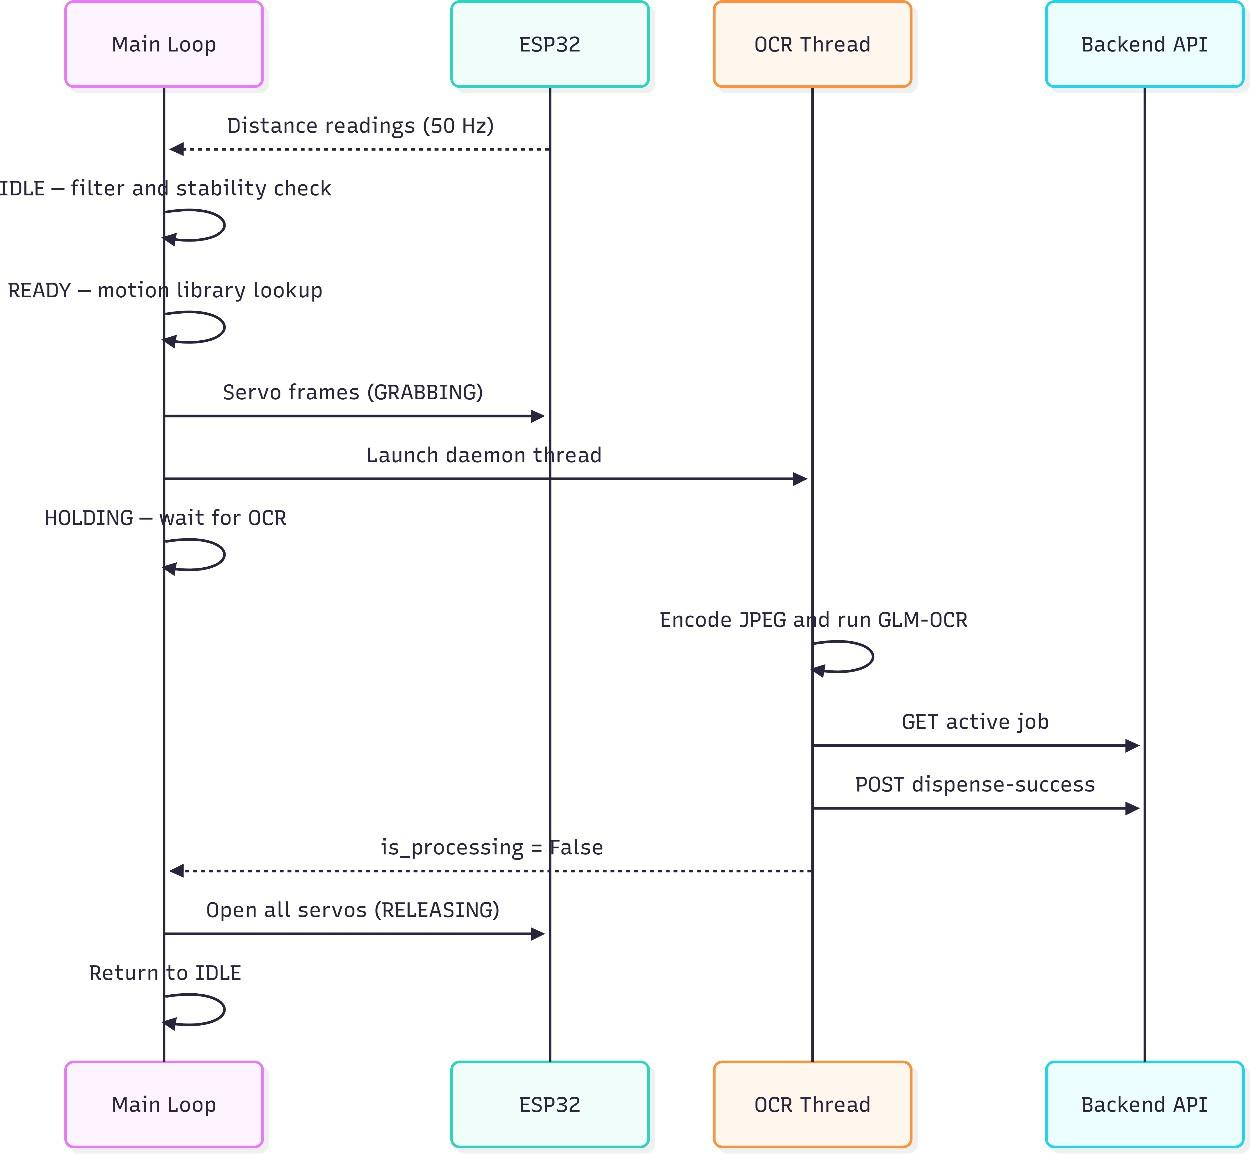
\includegraphics[width=4.55729in,height=4.20729in]{./media/image62.jpg}
\caption{Concurrency Timeline: Main Control Loop and Asynchronous VLM Daemon Thread\label{fig:fig18}}
\end{figure}

\section{Fullstack Screenshots and
Wireframes}\label{fullstack-screenshots-and-wireframes}

\subsection{PharmaSys Dashboard}\label{pharmasys-dashboard}

The PharmaSys staff interface is designed for desktop and tablet screens. It provides real-time status widgets, active order lists, and the AI command center.

\begin{figure}[htbp]
    \centering
    % Row 1: (a) Login Screen & (b) Main Overview Dashboard
    \begin{subfigure}[b]{0.48\textwidth}
        \centering
        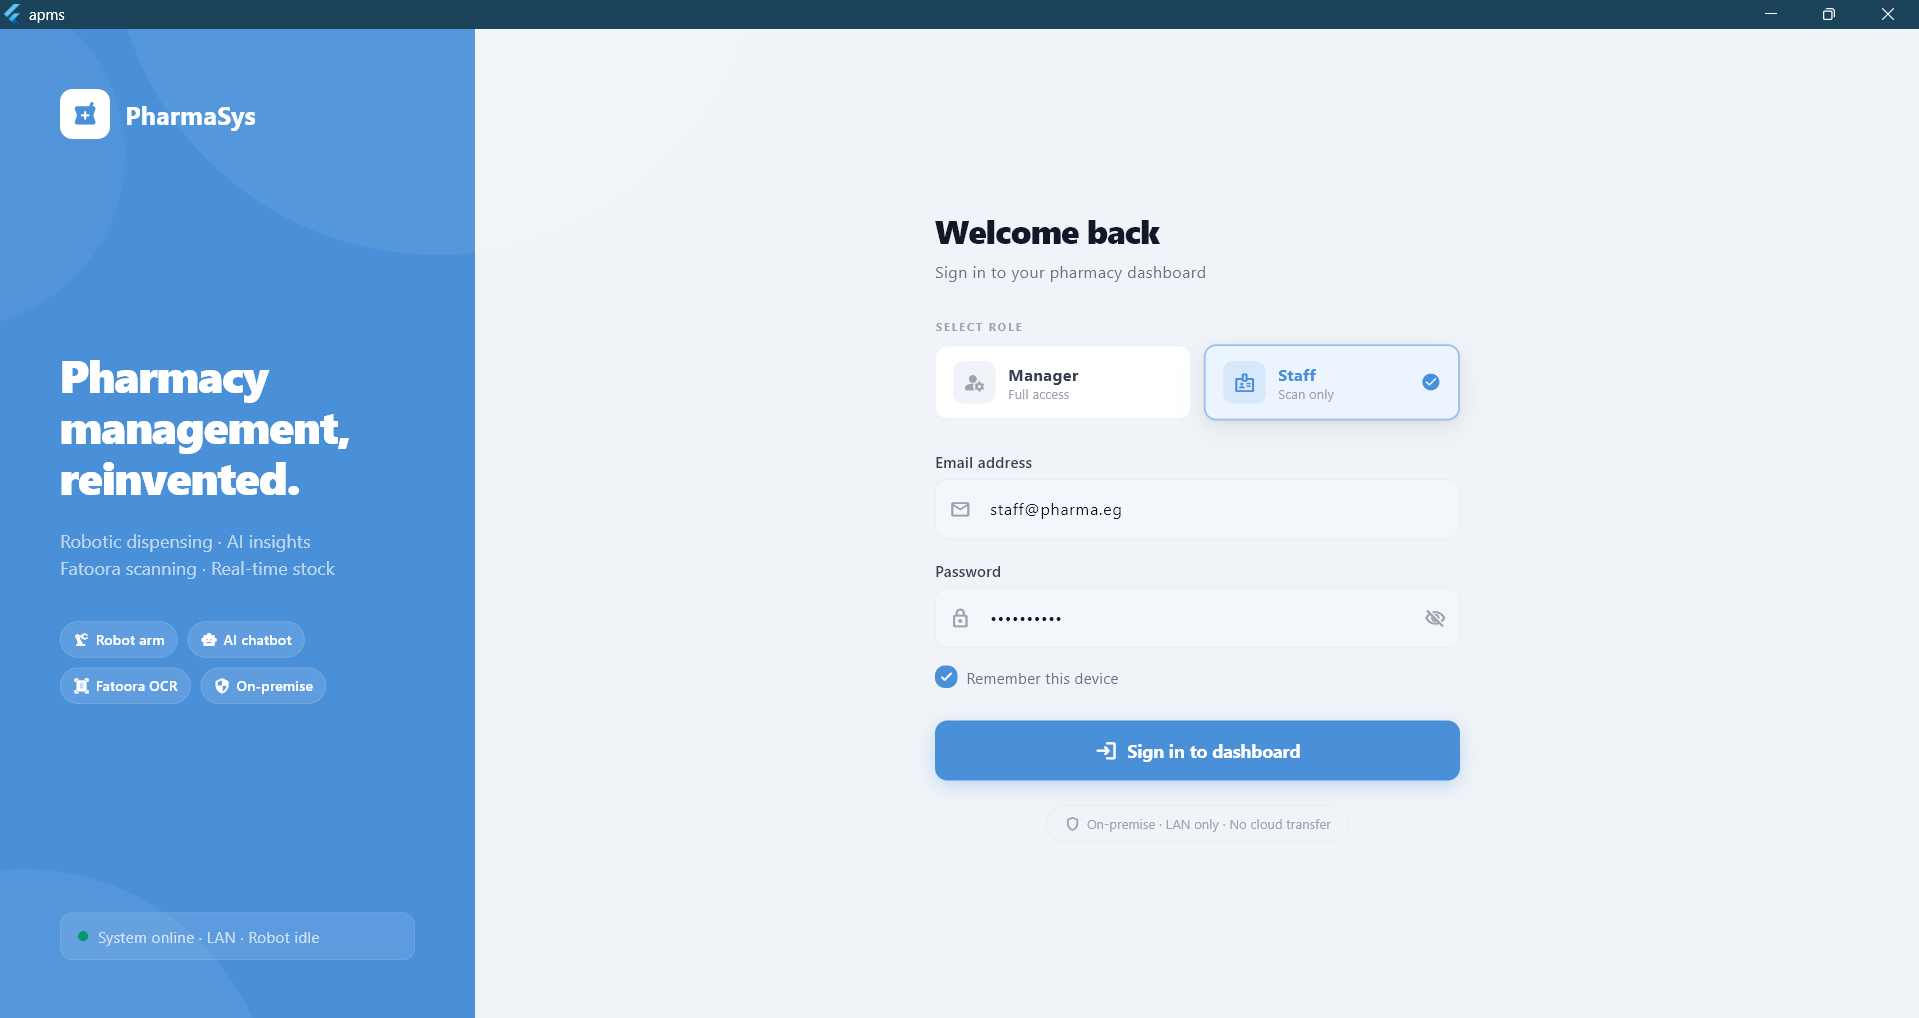
\includegraphics[width=\textwidth]{./media/image36.png}
        \caption{Login Screen}
    \end{subfigure}
    \hfill
    \begin{subfigure}[b]{0.48\textwidth}
        \centering
        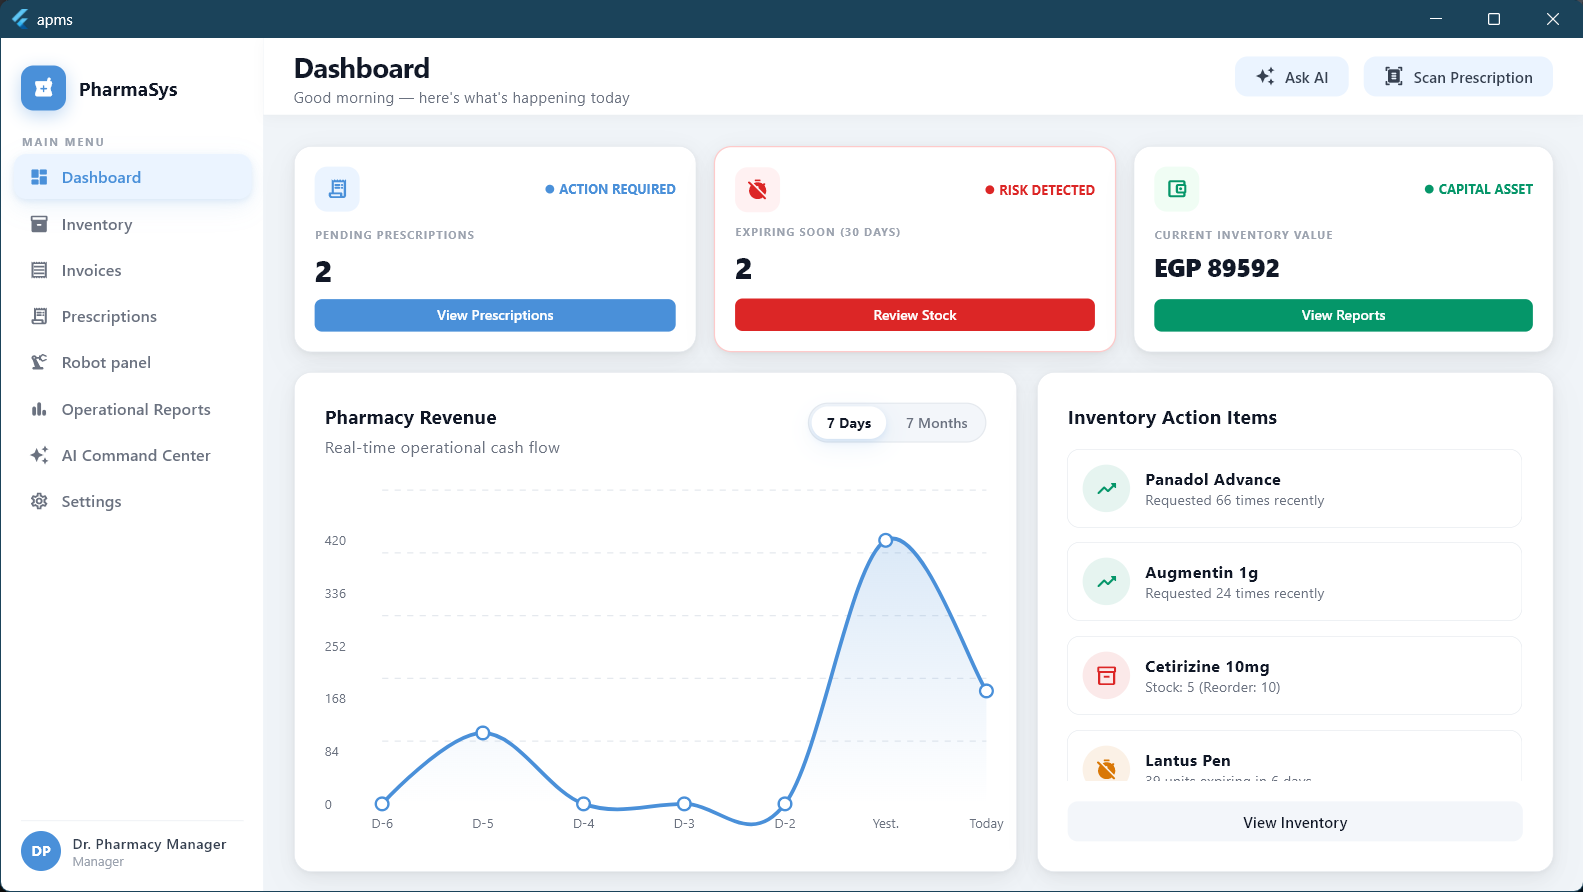
\includegraphics[width=\textwidth]{./media/image5.png}
        \caption{Main Overview Dashboard}
    \end{subfigure}
    
    \vspace{0.4cm}
    
    % Row 2: (c) Robot Panel & (d) Prescription Screen
    \begin{subfigure}[b]{0.48\textwidth}
        \centering
        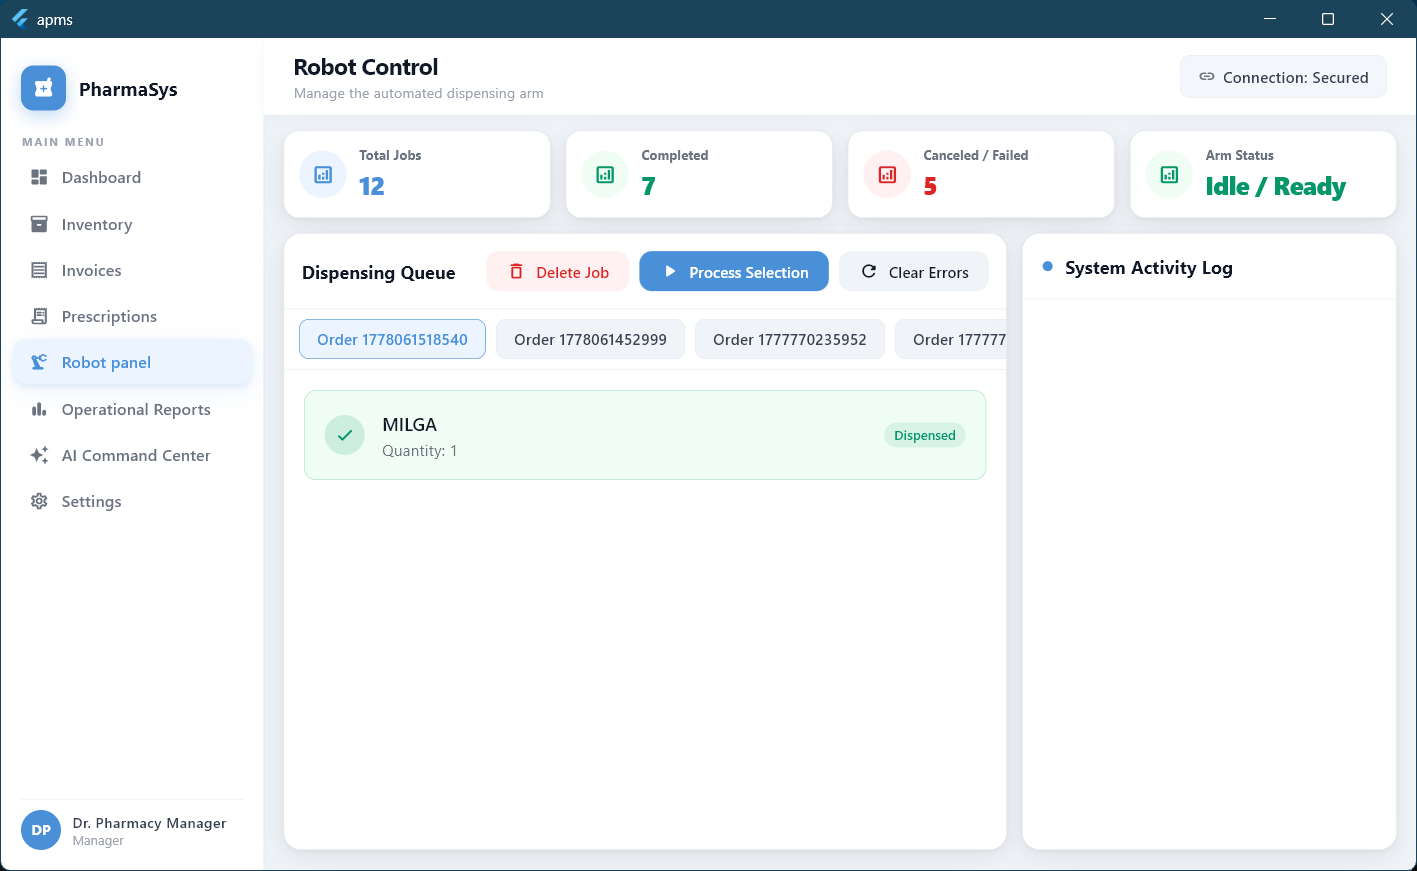
\includegraphics[width=\textwidth]{./media/image12.png}
        \caption{Robot Panel}
    \end{subfigure}
    \hfill
    \begin{subfigure}[b]{0.48\textwidth}
        \centering
        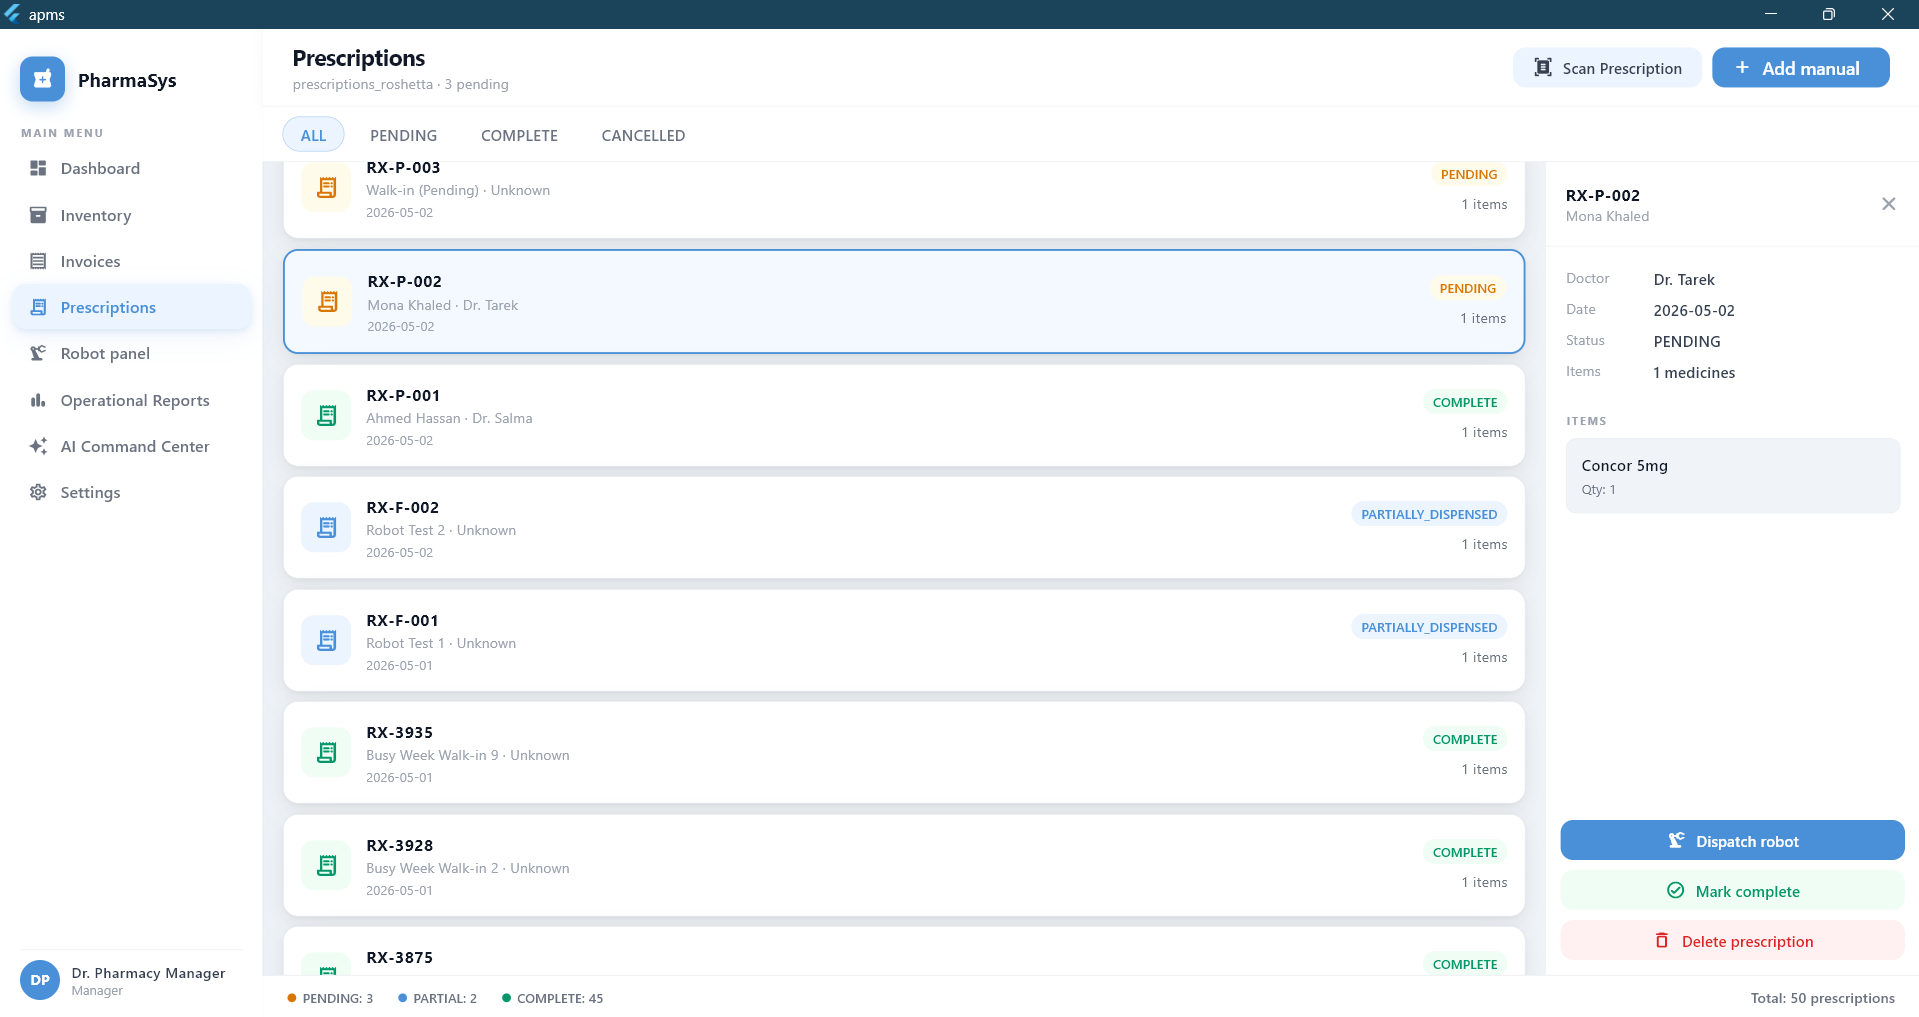
\includegraphics[width=\textwidth]{./media/image11.png}
        \caption{Prescription Screen}
    \end{subfigure}
    
    \vspace{0.4cm}
    
    % Row 3: (e) Medicines Inventory Stock & (f) Invoice Screen
    \begin{subfigure}[b]{0.48\textwidth}
        \centering
        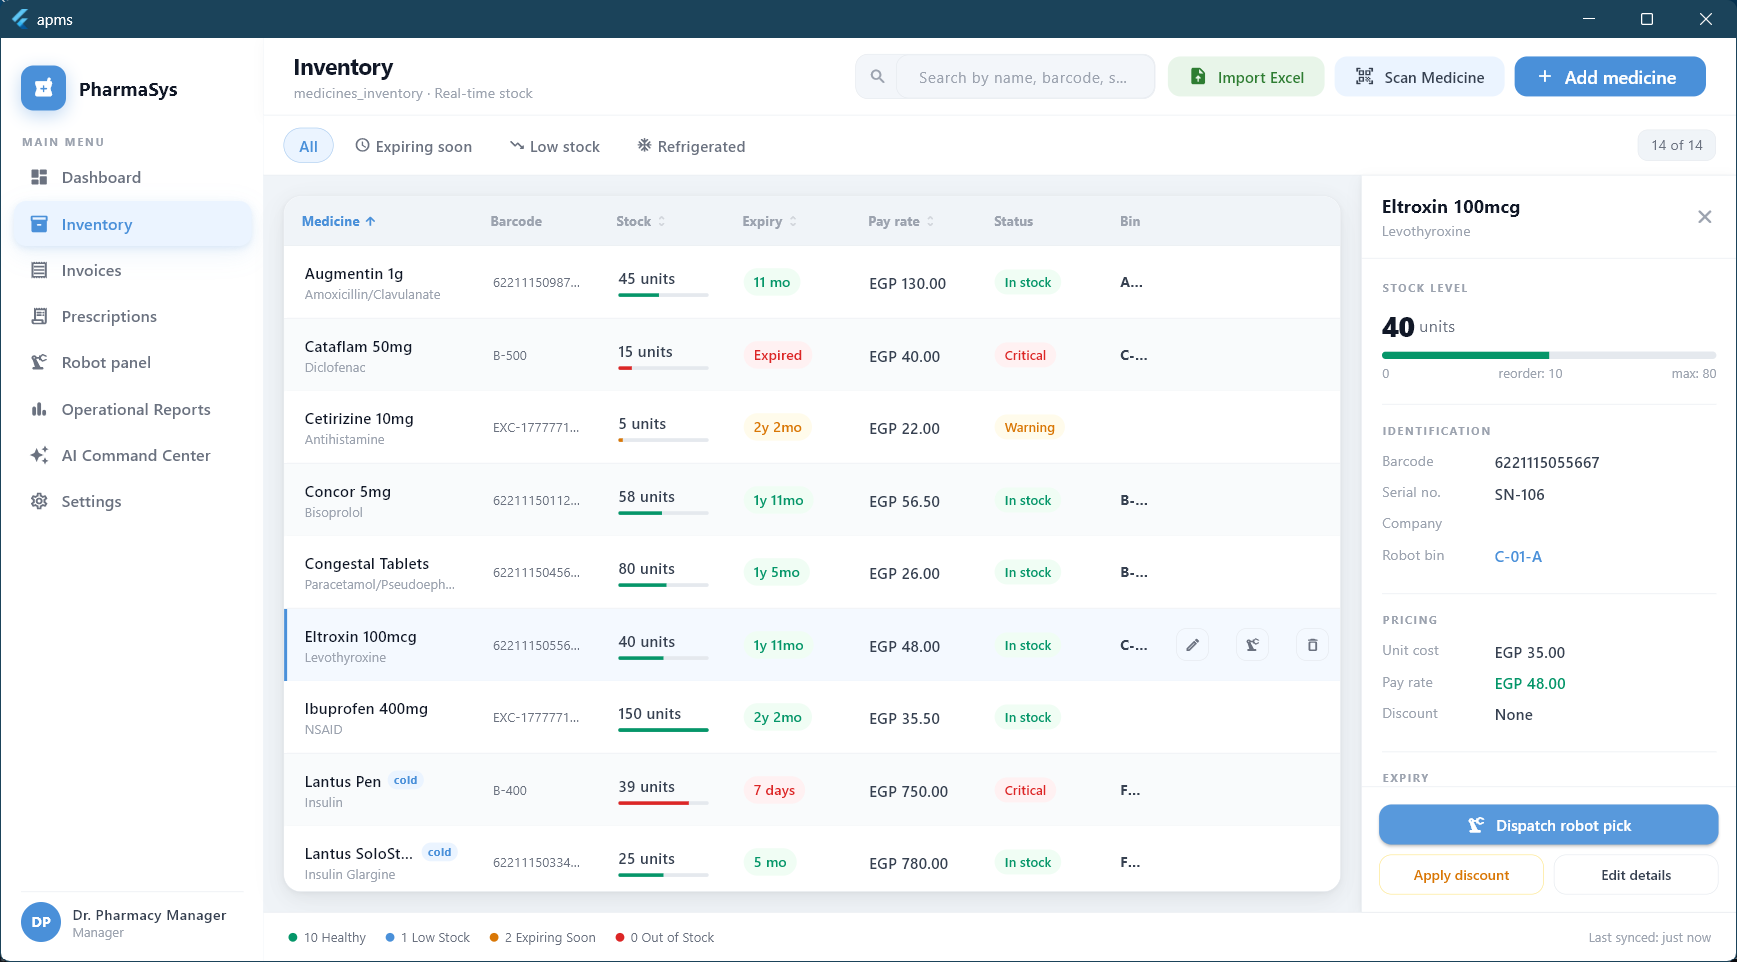
\includegraphics[width=\textwidth]{./media/image38.png}
        \caption{Medicines Inventory Stock}
    \end{subfigure}
    \hfill
    \begin{subfigure}[b]{0.48\textwidth}
        \centering
        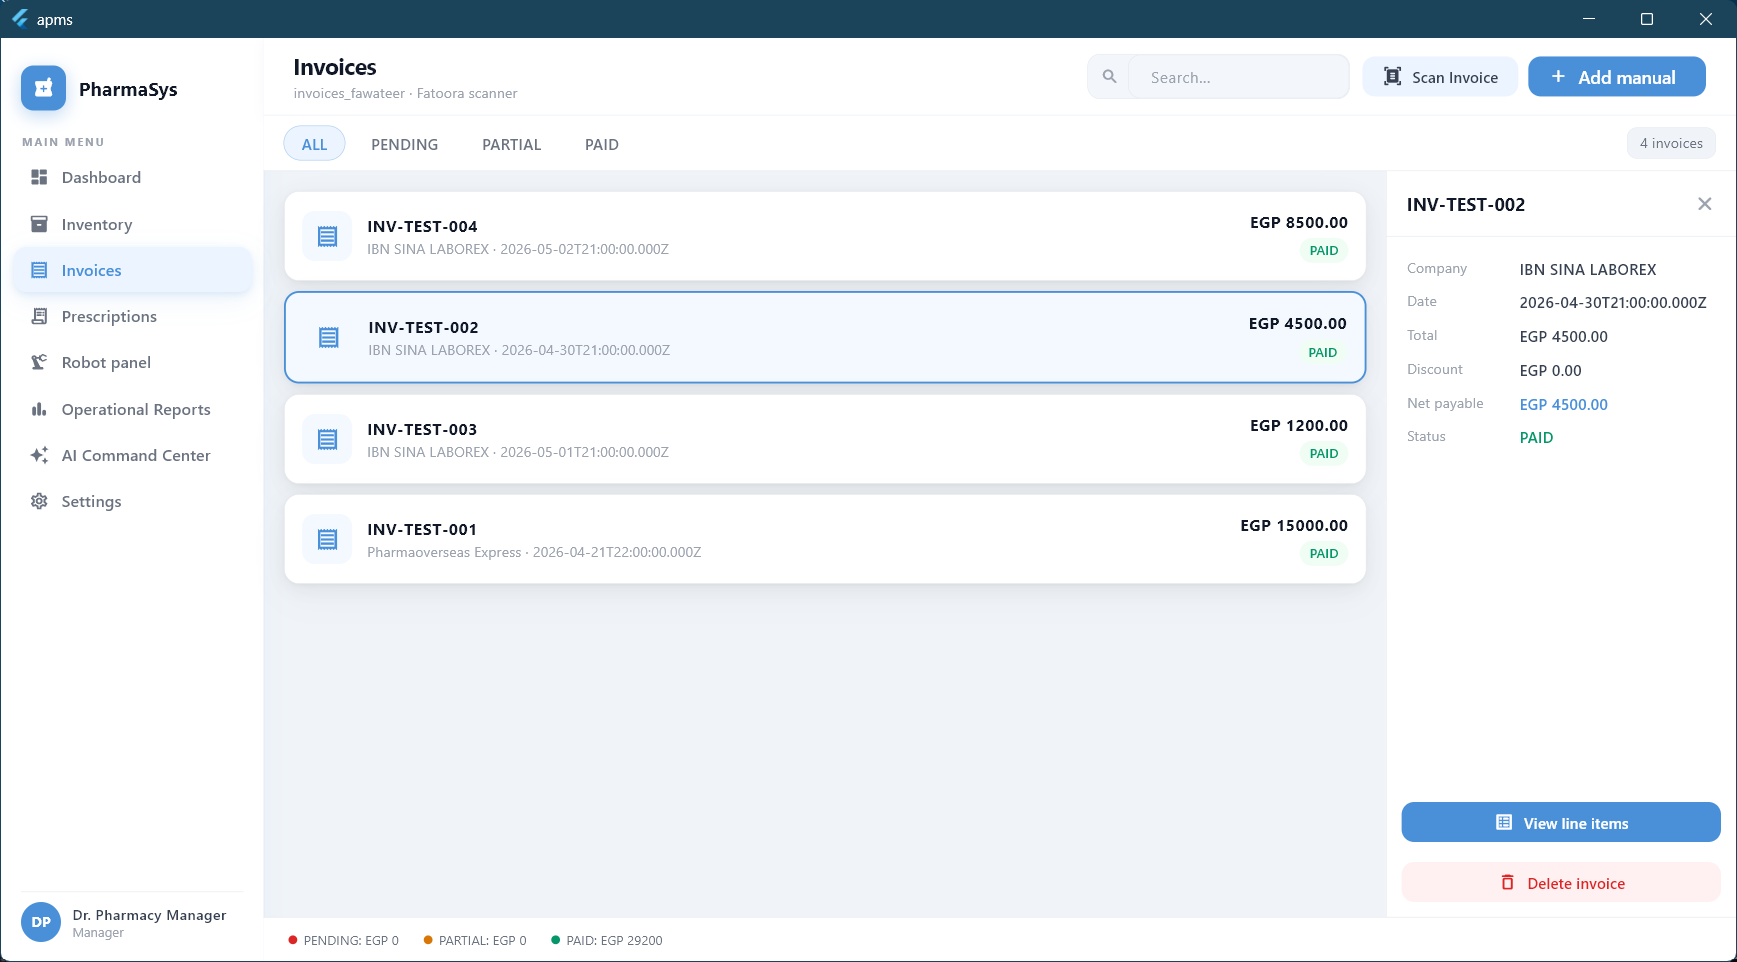
\includegraphics[width=\textwidth]{./media/image22.png}
        \caption{Invoice Screen}
    \end{subfigure}
    
    \caption{PharmaSys Staff Enterprise Interfaces}
    \label{fig:fig19}
\end{figure}
\subsection{Roshetety Patient Mobile App}\label{roshetety-patient-mobile-app}

Roshetety allows patients to capture prescriptions, select medicines, and track their preparation progress.

\begin{figure}[htbp]
    \centering
    % Row 1
    \begin{subfigure}[b]{0.23\textwidth}
        \centering
        
\includegraphics[width=\textwidth]{./media/image20.jpg} % Swapped to match image
        \caption{Splash Screen}
    \end{subfigure}
    \hfill
    \begin{subfigure}[b]{0.23\textwidth}
        \centering
        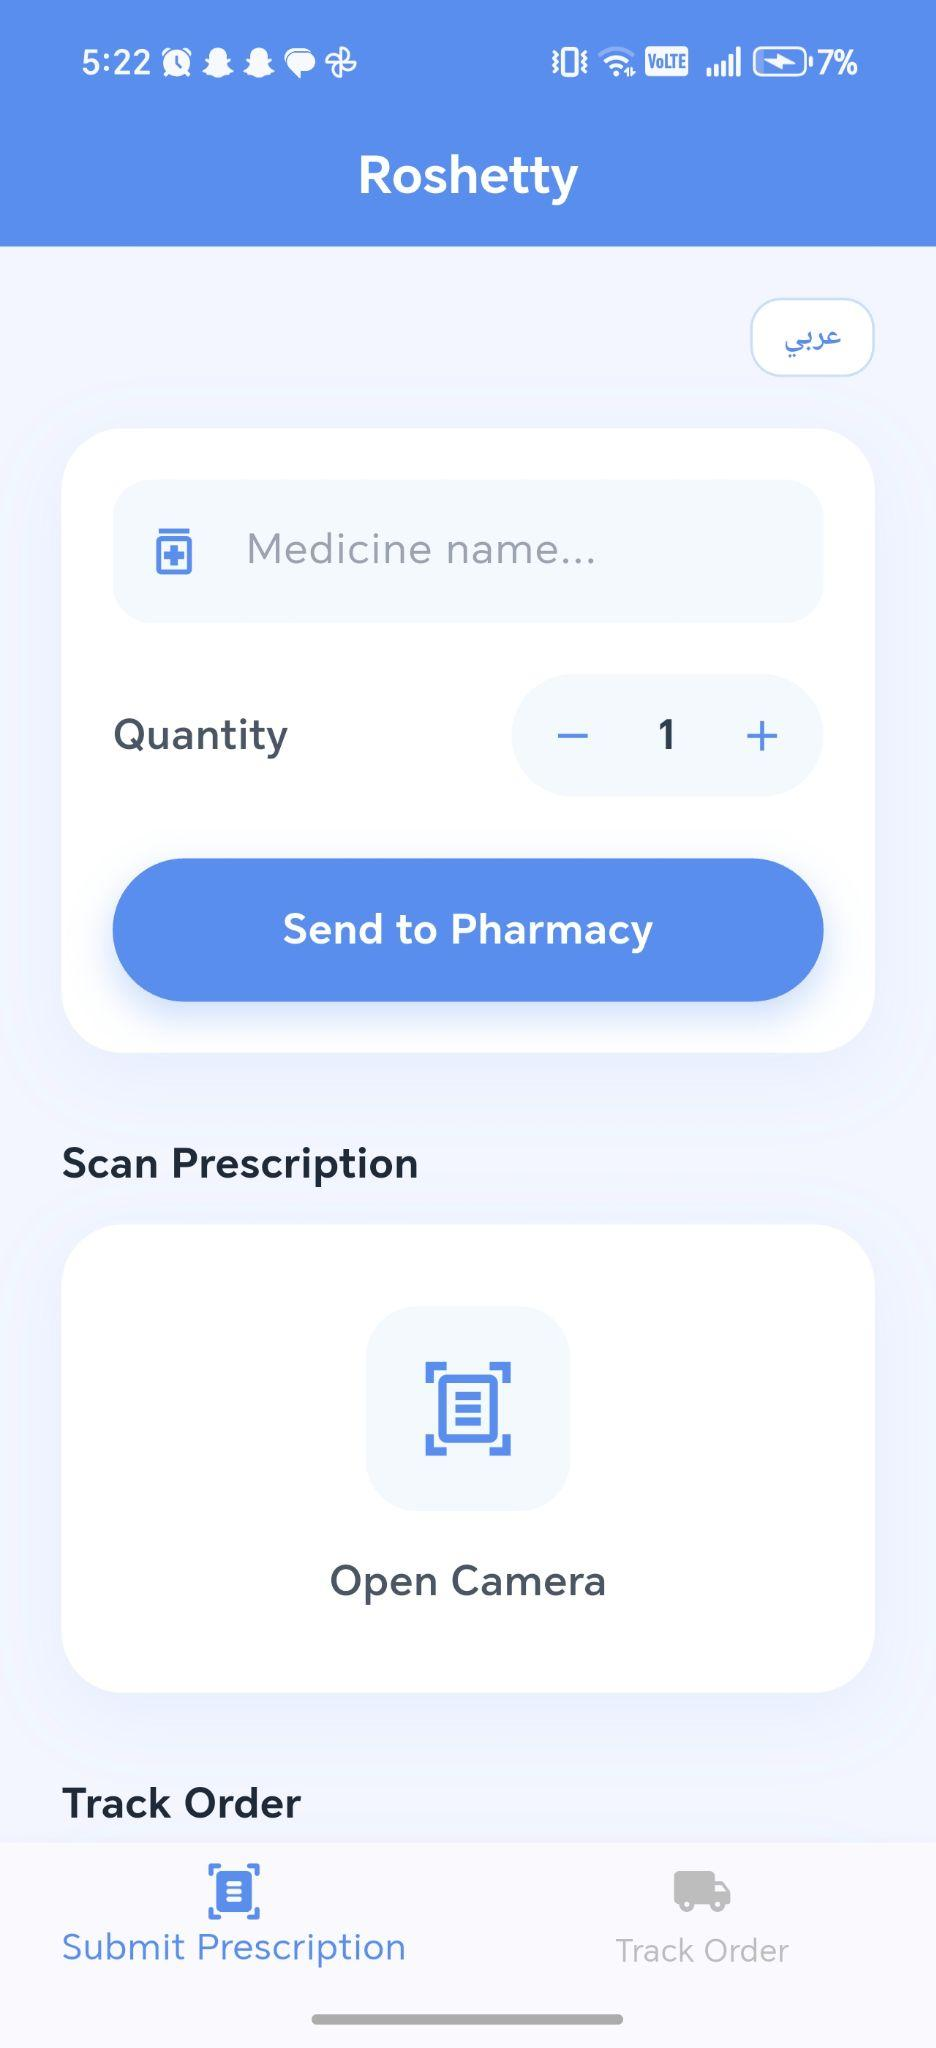
\includegraphics[width=\textwidth]{./media/image9.jpg}
        \caption{Homepage}
    \end{subfigure}
    \hfill
    \begin{subfigure}[b]{0.23\textwidth}
        \centering
        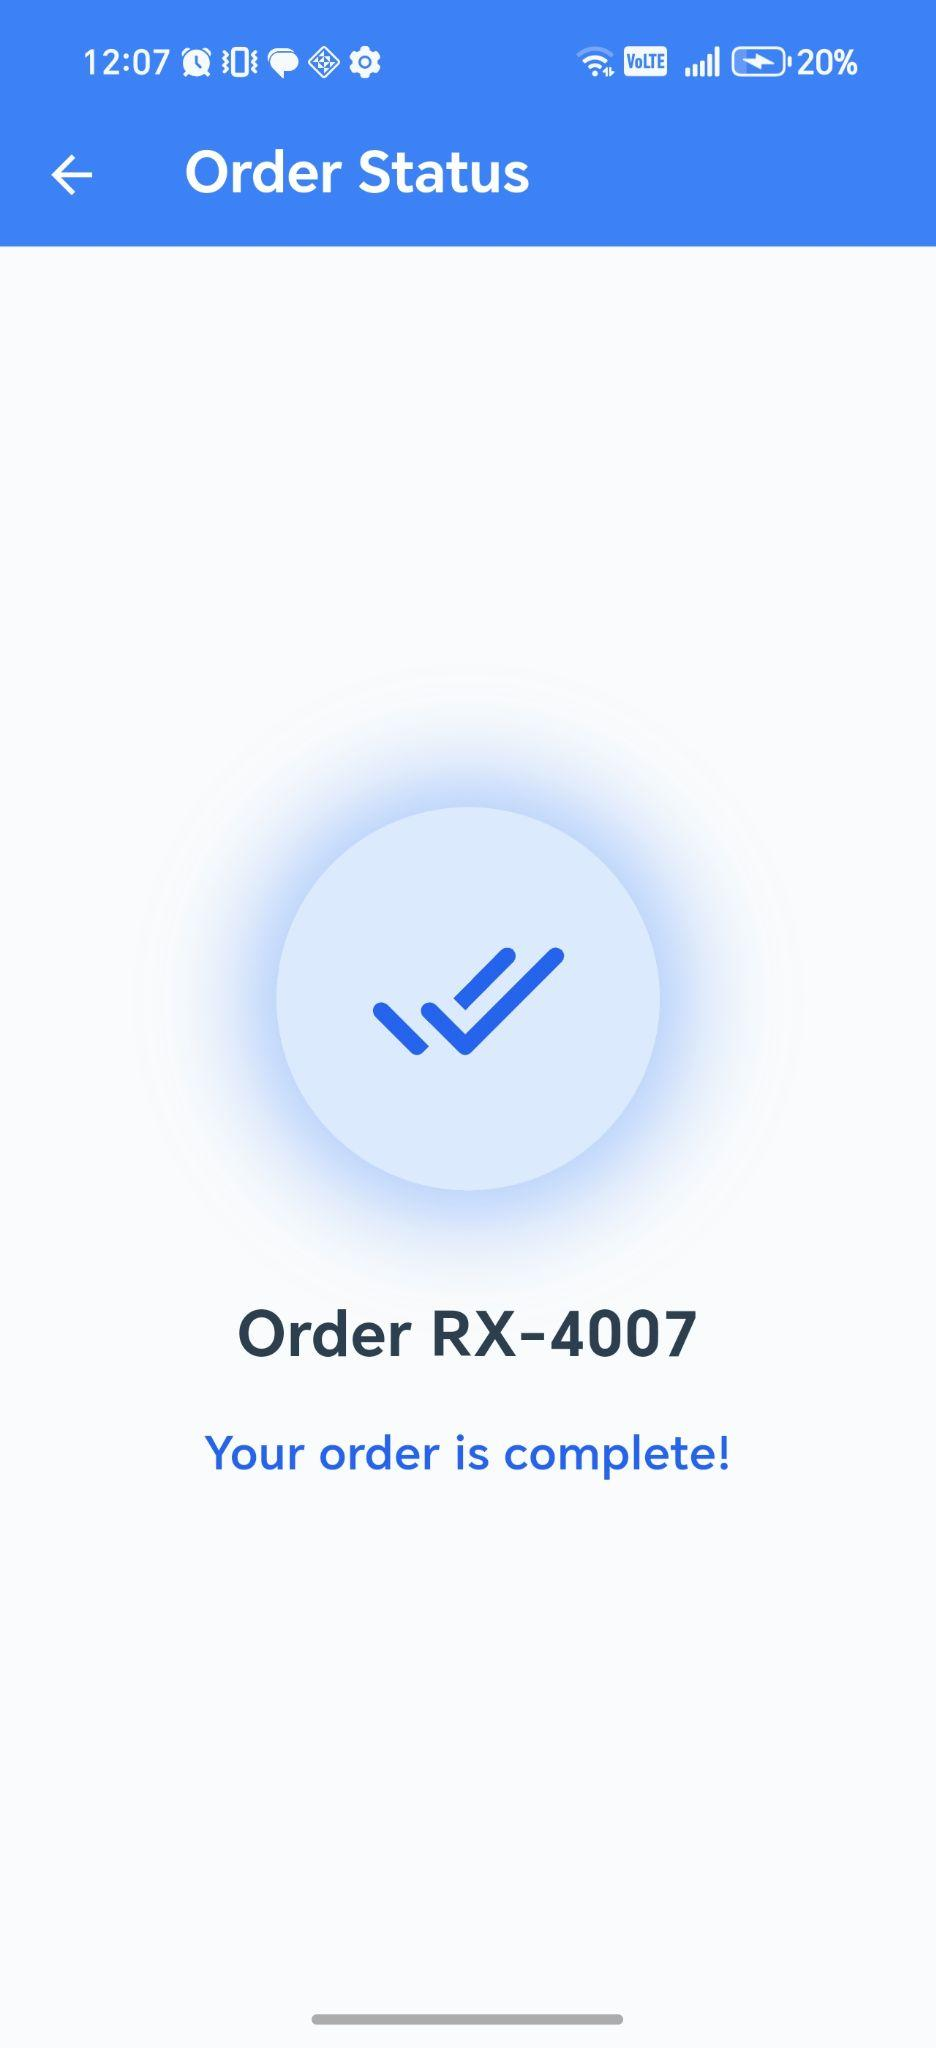
\includegraphics[width=\textwidth]{./media/image34.jpg} % Swapped to match image
        \caption{Order Completed}
    \end{subfigure}
    \hfill
    \begin{subfigure}[b]{0.23\textwidth}
        \centering
        
\includegraphics[width=\textwidth]{./media/image3.jpg}
        \caption{Prescription Capture}
    \end{subfigure}
    
    \vspace{0.4cm}
    
    % Row 2
    \begin{subfigure}[b]{0.23\textwidth}
        \centering
        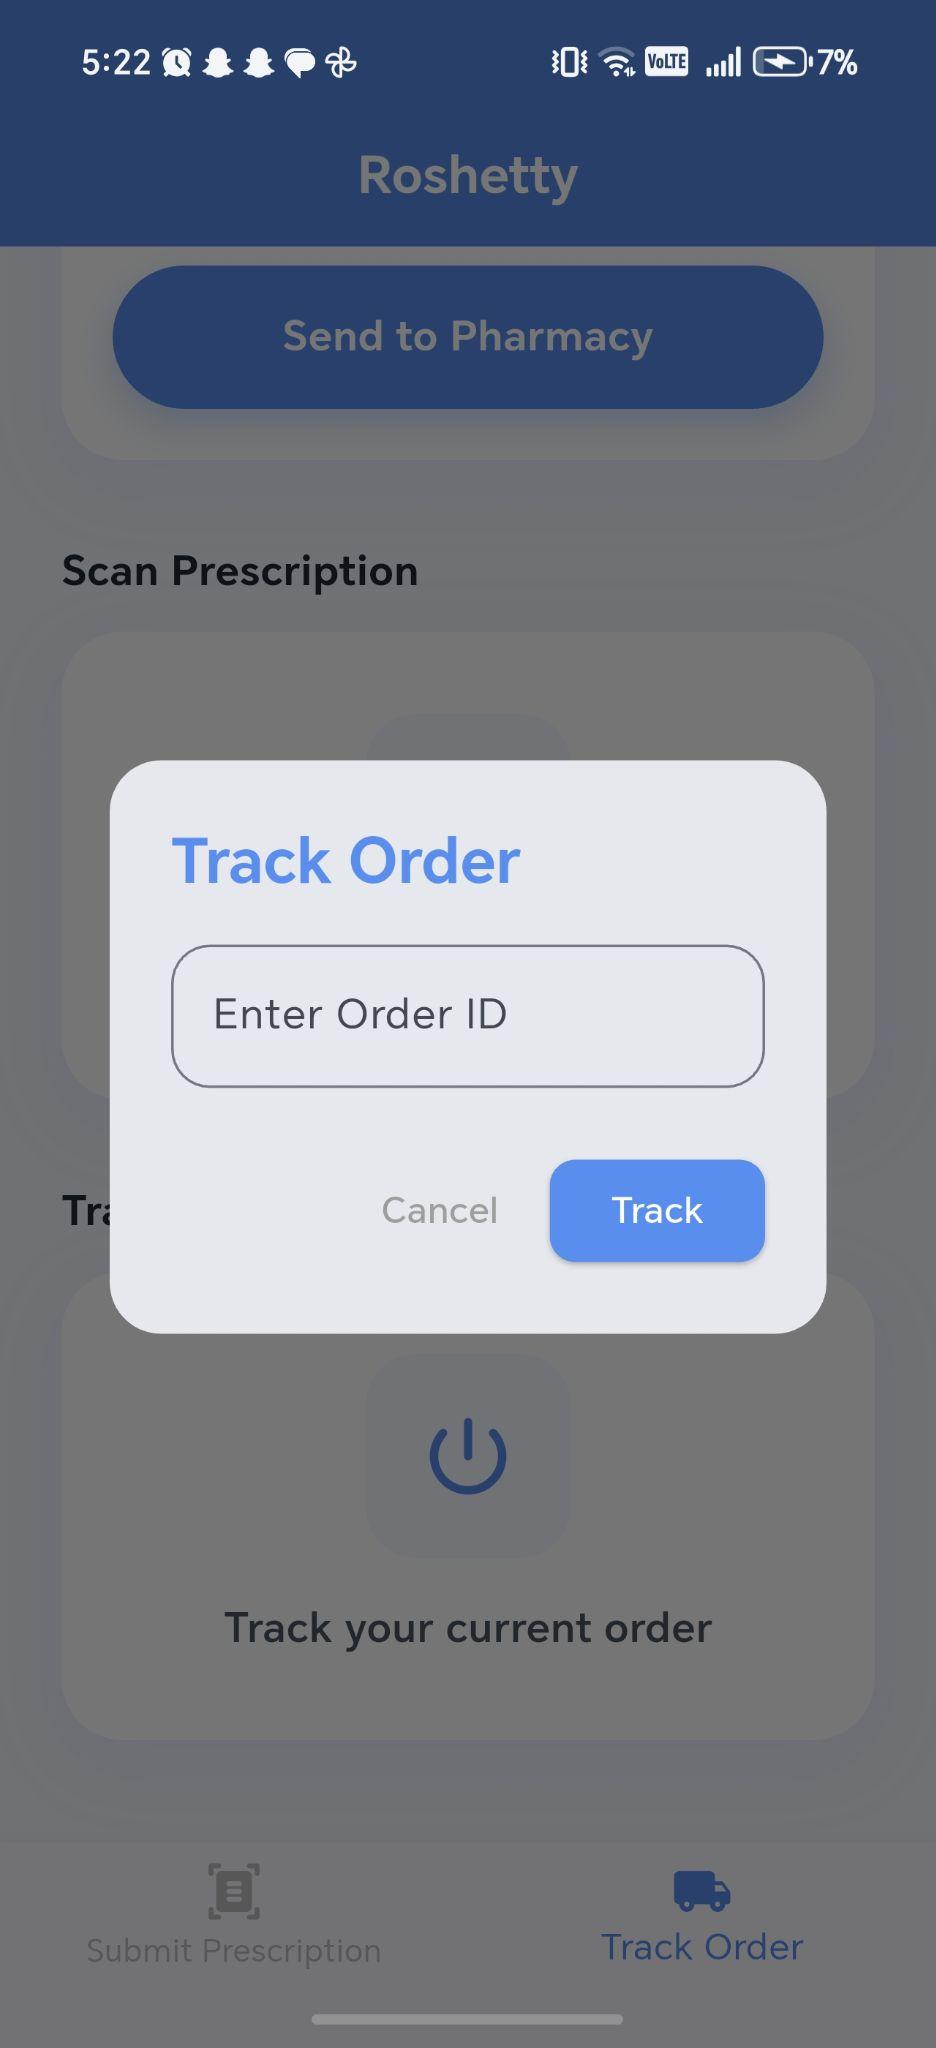
\includegraphics[width=\textwidth]{./media/image69.jpg}
        \caption{Order Tracking}
    \end{subfigure}
    \quad
    \begin{subfigure}[b]{0.23\textwidth}
        \centering
        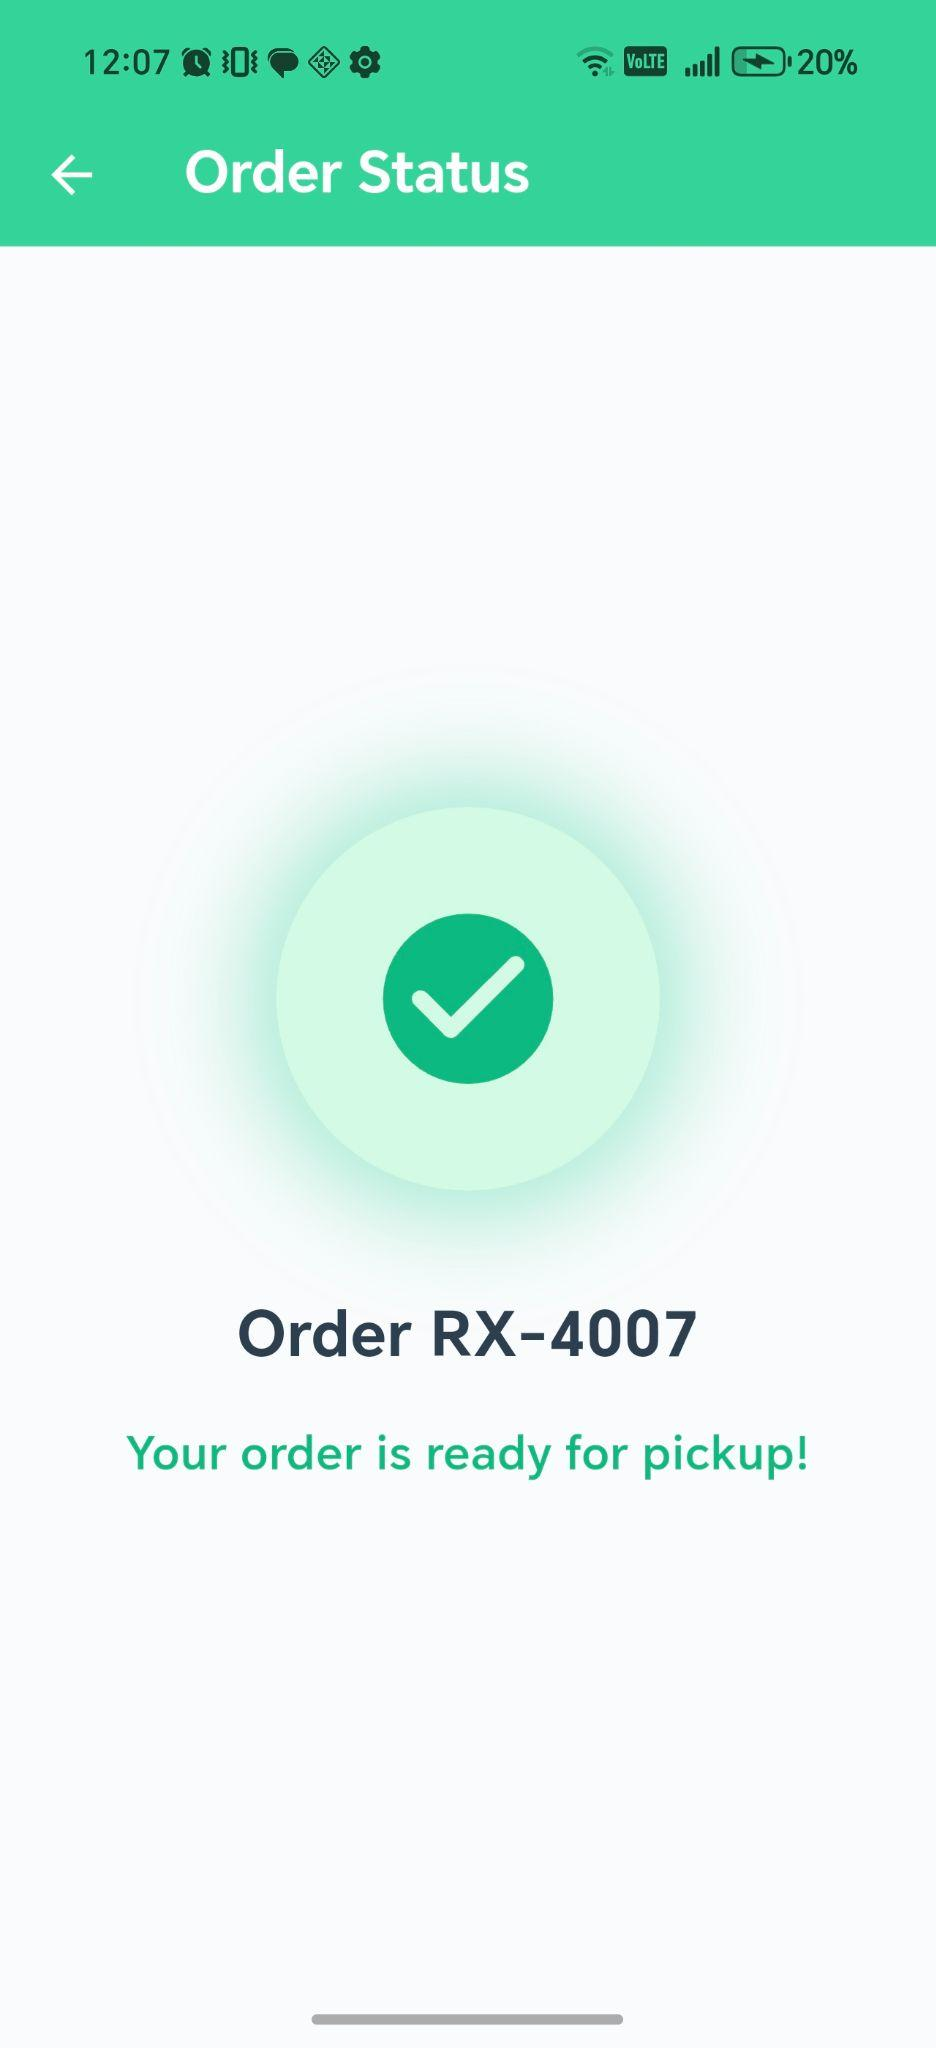
\includegraphics[width=\textwidth]{./media/image47.jpg}
        \caption{Order Dispatched}
    \end{subfigure}
    \quad
    \begin{subfigure}[b]{0.23\textwidth}
        \centering
        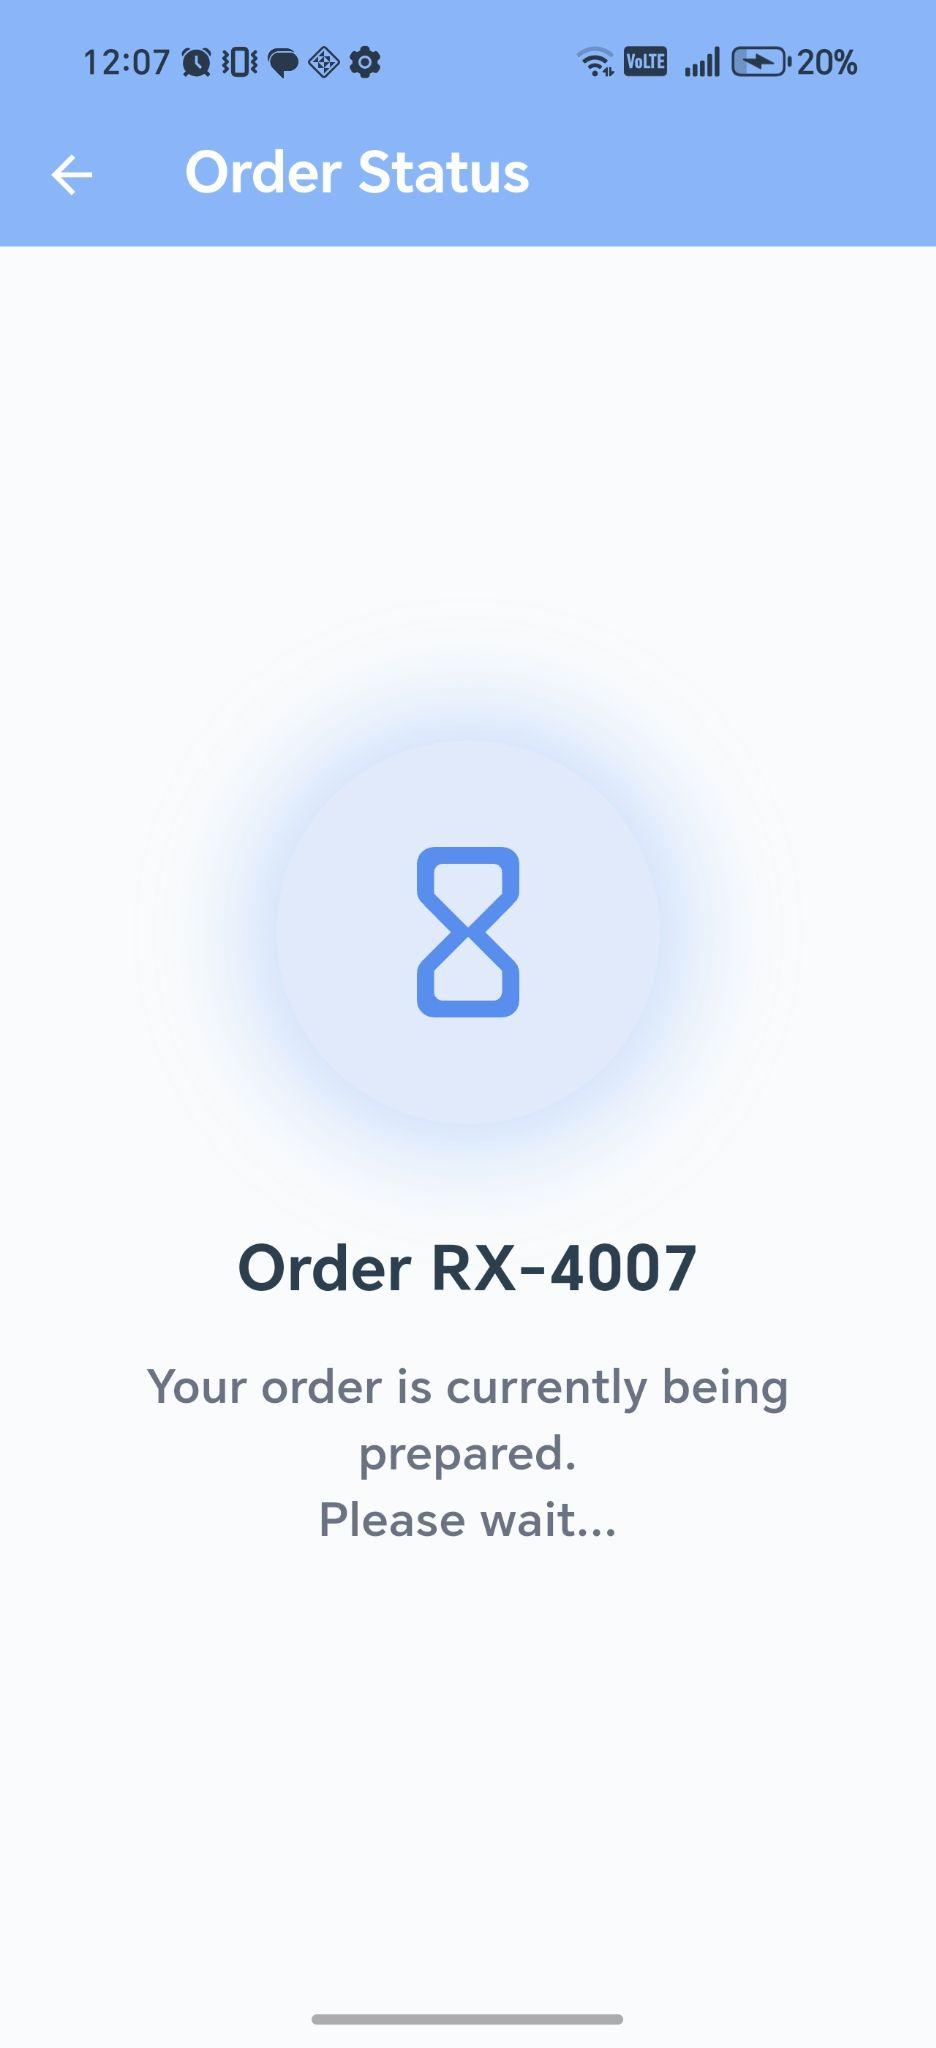
\includegraphics[width=\textwidth]{./media/image58.jpg} 
        \caption{order waitlisting}
    \end{subfigure}
    
    \caption{Roshetety Mobile App Client Screens}
    \label{fig:fig20}
\end{figure}

\section{AI Command Center Screenshots}\label{ai-command-center-screenshots}

The AI analytics outputs are integrated as a dedicated command center within PharmaSys:

\begin{figure}[htbp]
    \centering
    \begin{subfigure}[b]{0.48\textwidth}
        \centering
        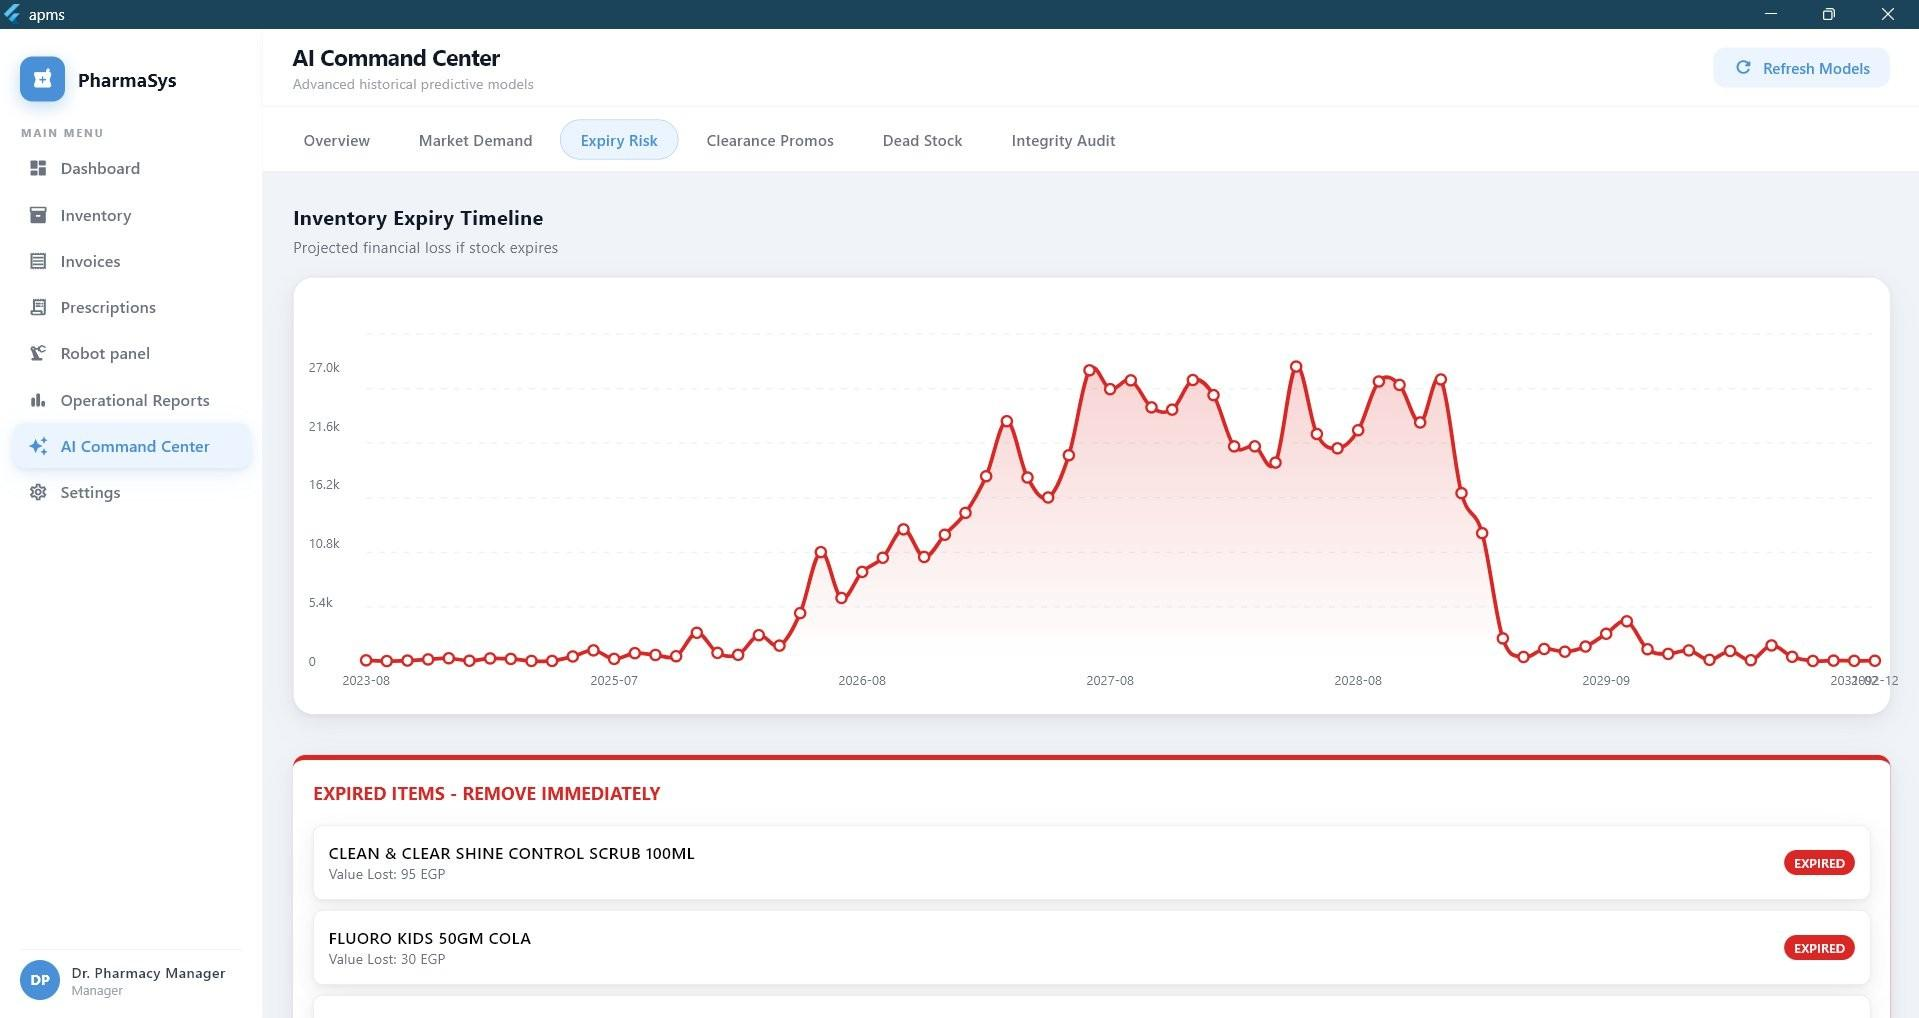
\includegraphics[width=\textwidth]{./media/image2.jpg}
        \caption{Market Demand \& Near-Stockout}
    \end{subfigure}
    \hfill
    \begin{subfigure}[b]{0.48\textwidth}
        \centering
        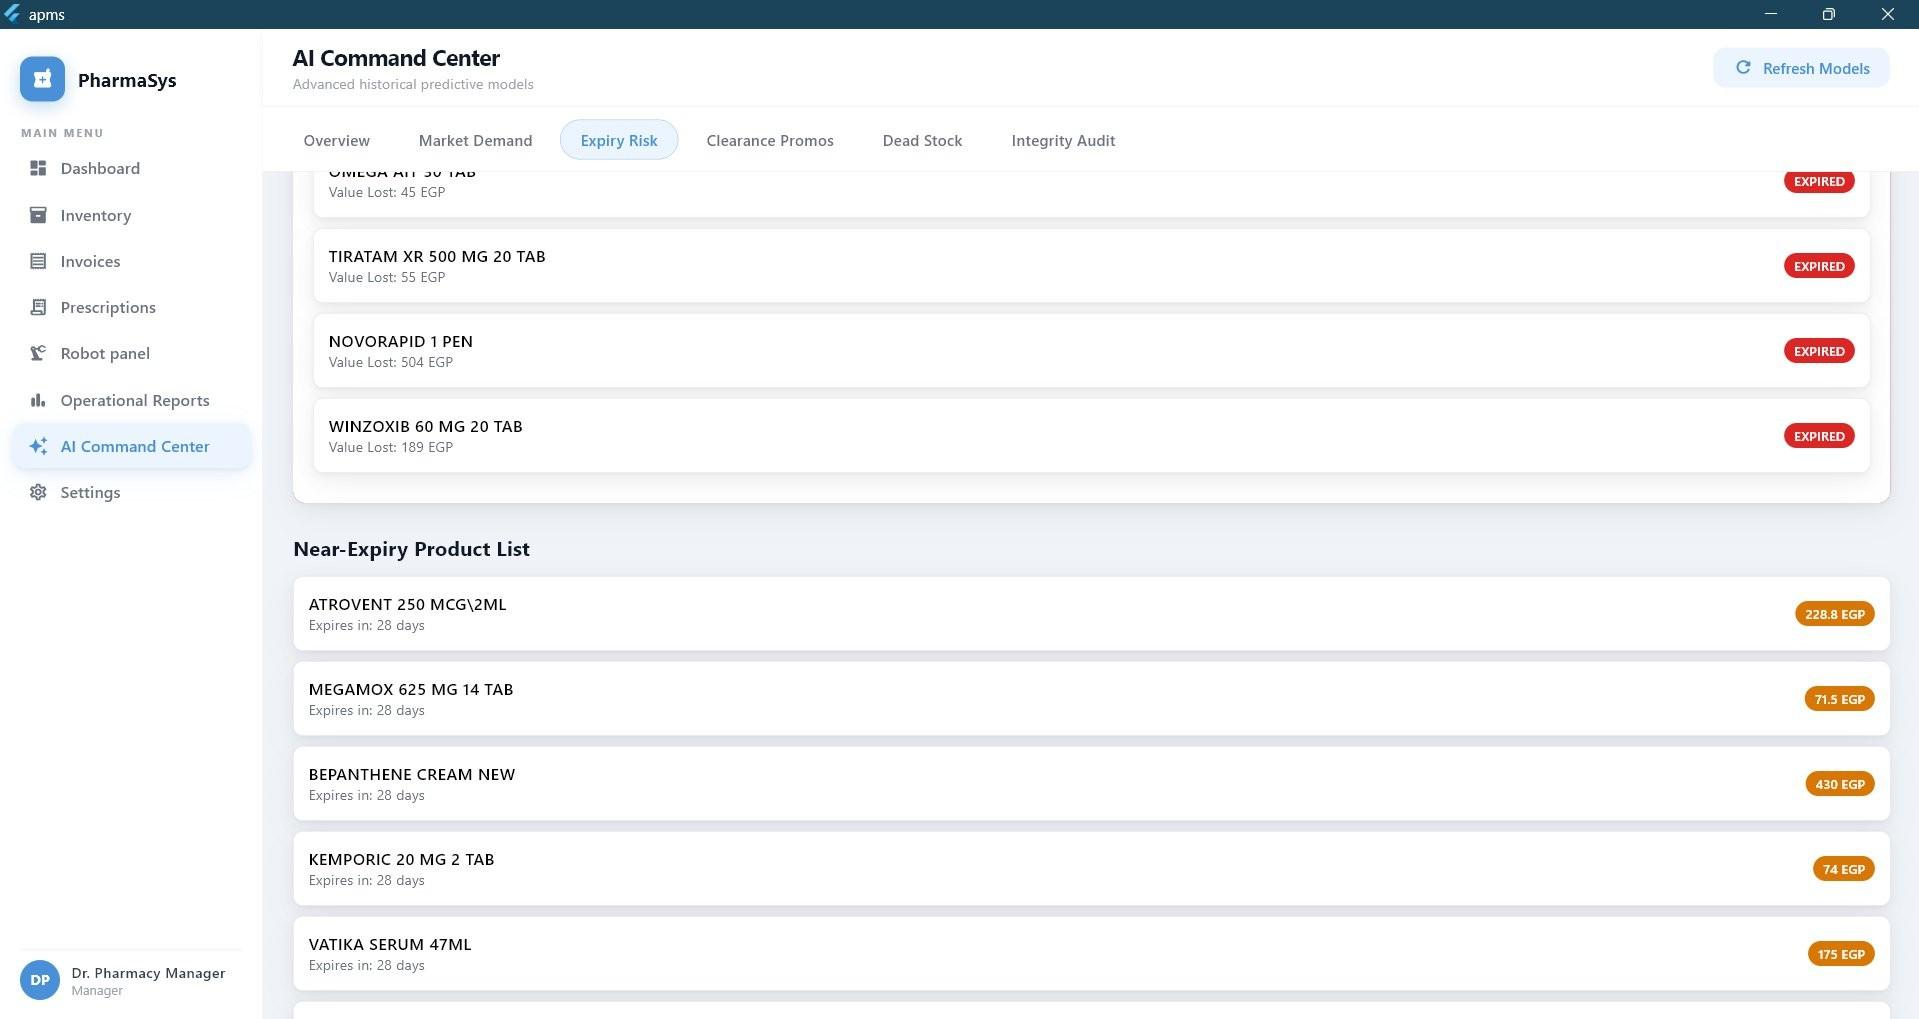
\includegraphics[width=\textwidth]{./media/image10.jpg}
        \caption{Expiry Risk Timeline}
    \end{subfigure}
    
    \vspace{0.4cm}
    
    \begin{subfigure}[b]{0.48\textwidth}
        \centering
        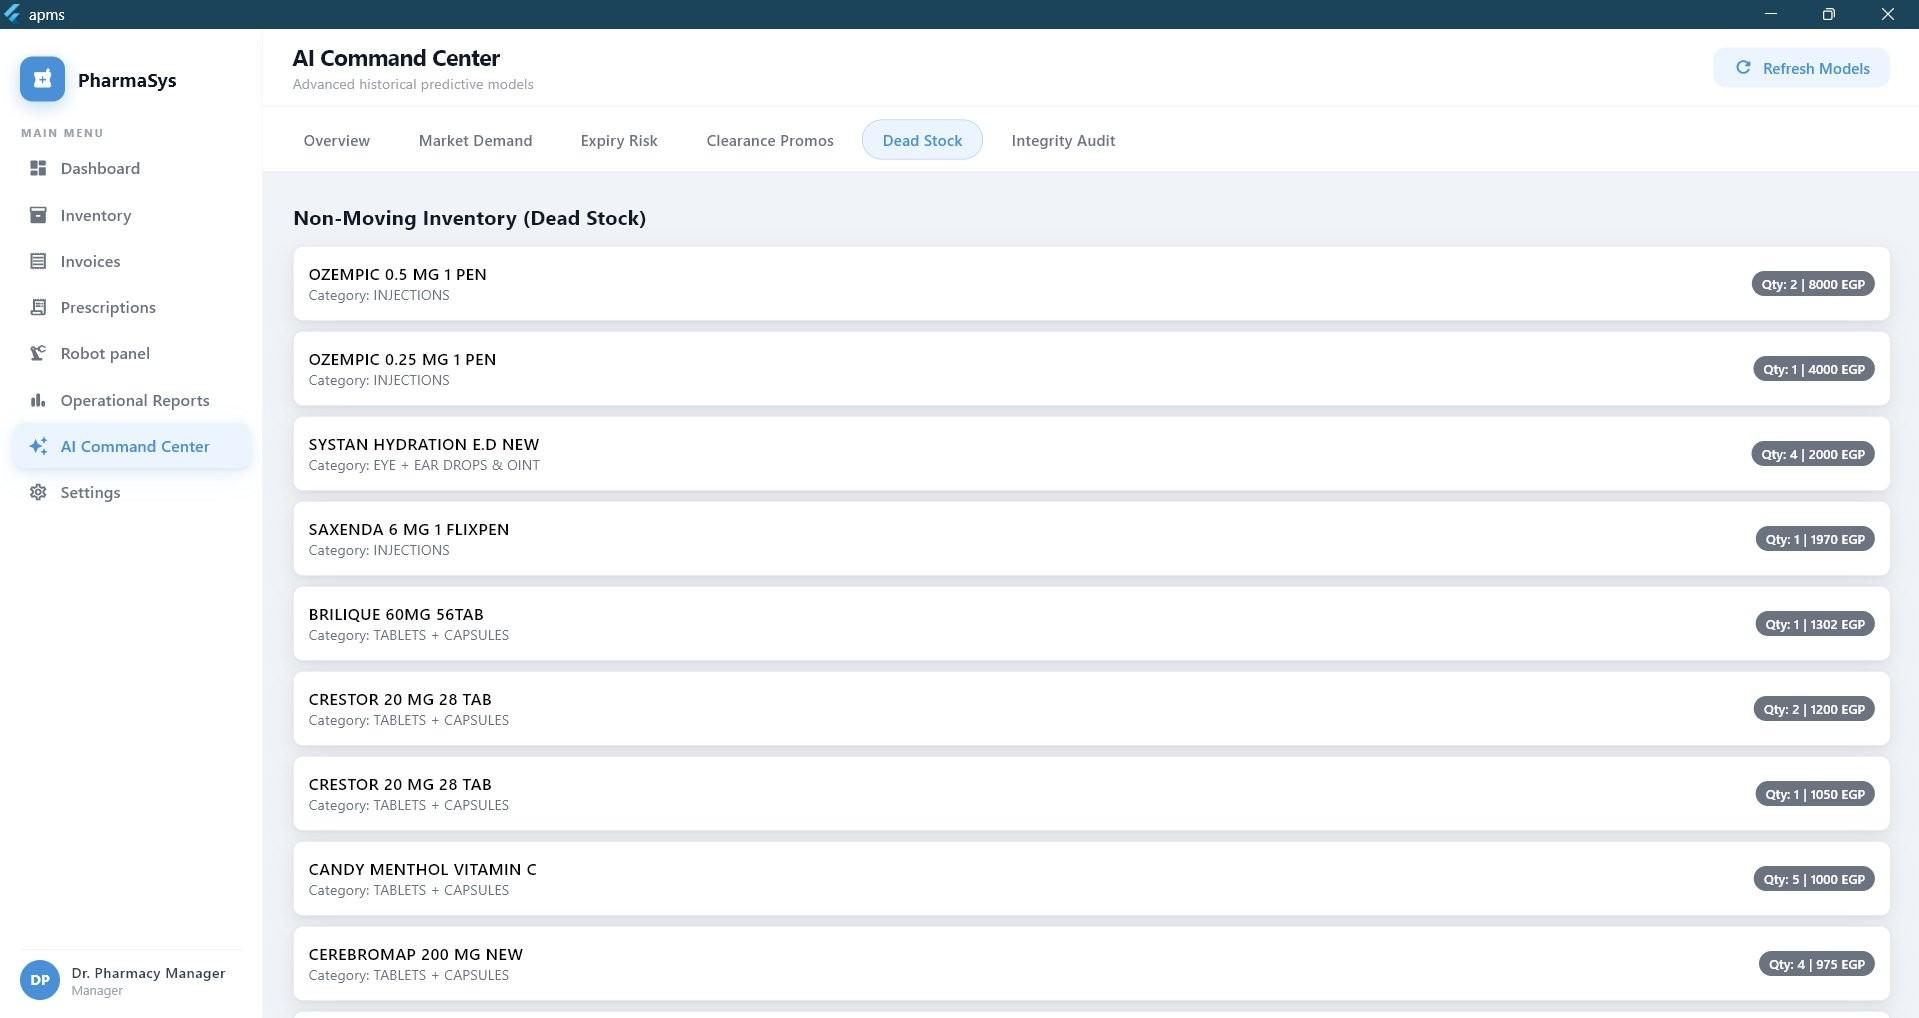
\includegraphics[width=\textwidth]{./media/image19.jpg}
        \caption{Clearance Discount Recommendations}
    \end{subfigure}
    \hfill
    \begin{subfigure}[b]{0.48\textwidth}
        \centering
        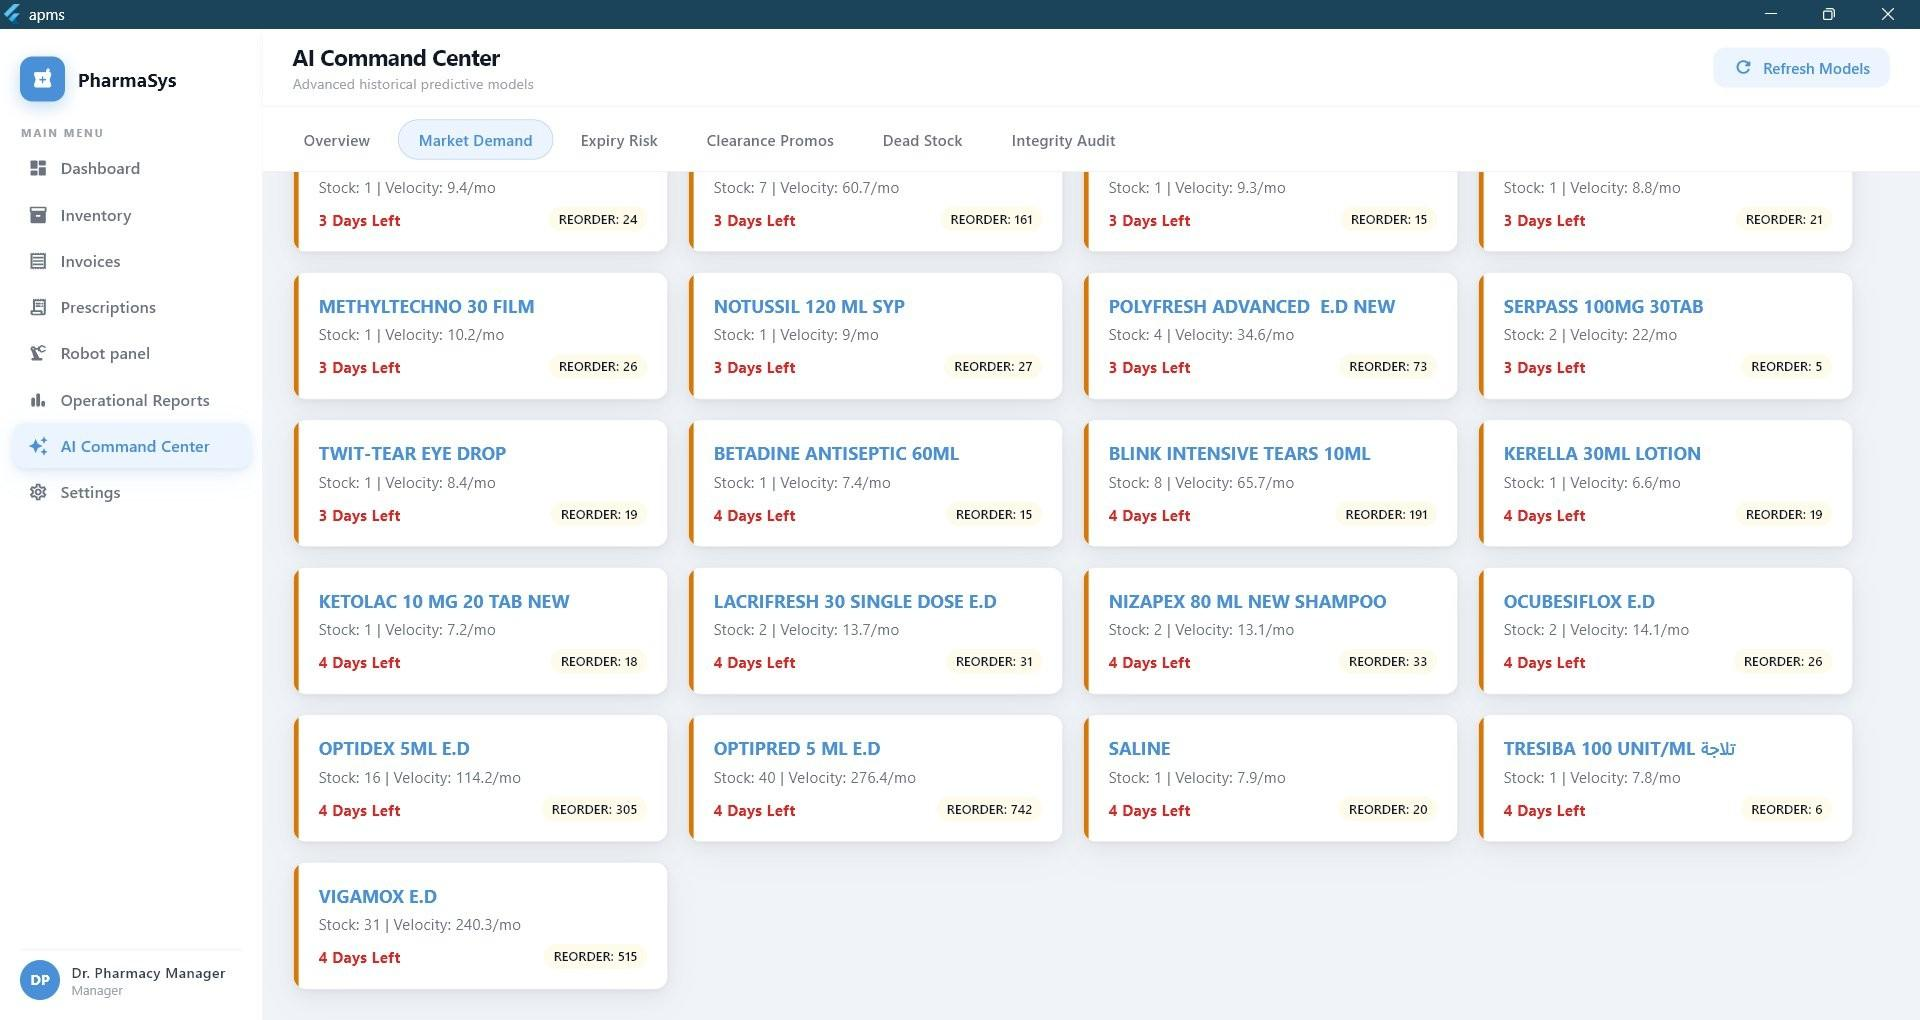
\includegraphics[width=\textwidth]{./media/image26.jpg}
        \caption{Dead Stock \& Non-Moving Inventory}
    \end{subfigure}
    \begin{subfigure}[b]{0.48\textwidth}
        \centering
        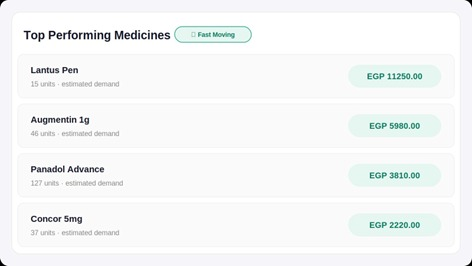
\includegraphics[width=\textwidth]{./media/ghada-fig1.jpeg}
        \caption{Top Performing Medicines.}
    \end{subfigure}
    \begin{subfigure}[b]{0.48\textwidth}
        \centering
        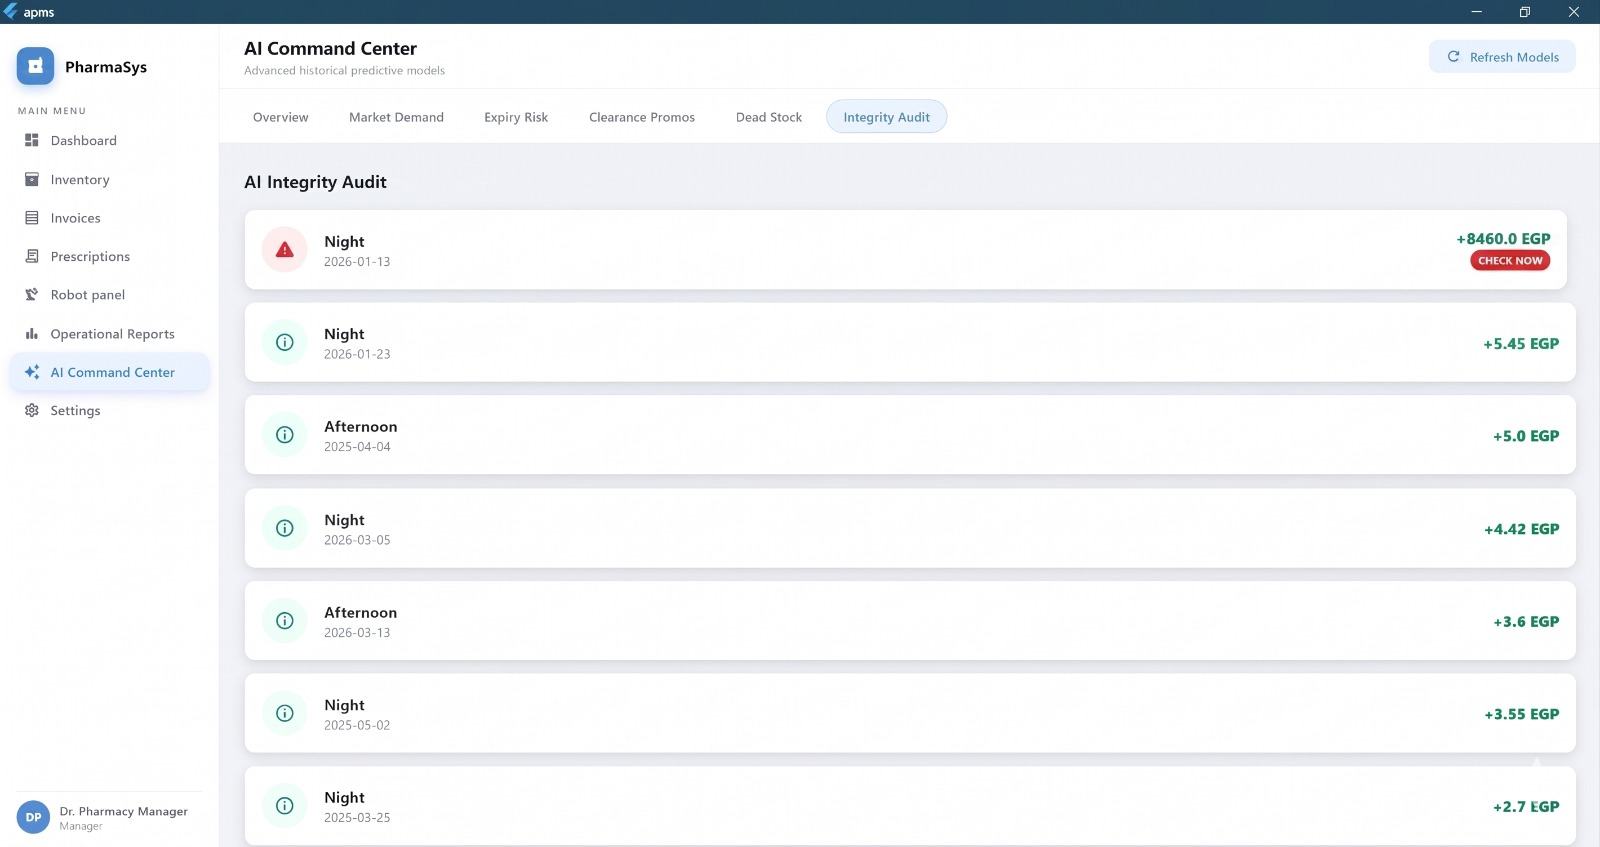
\includegraphics[width=\textwidth]{./media/ghada-fig3.jpeg}
        \caption{Anomaly detection.}
    \end{subfigure}
    \caption{APMS AI Command Center Widgets}
    \label{fig:fig21}
\end{figure}
\section{Experimental Results and
Discussion}\label{experimental-results-and-discussion}

\subsection{Robotic Grasping Success
Rates}\label{robotic-grasping-success-rates}

We evaluated the physical robotic hand grasping accuracy on typical
medicine boxes (MILGA, NEXICURE, STATURIC, EXAMIDE) across 300
experimental trials (50 trials per distance step). A grasp is classified
as successful if the hand grabs the package, lifts it, and retains it
for 6 seconds without slippage.

\begin{longtable}[]{@{}
  >{\raggedright\arraybackslash}p{(\linewidth - 6\tabcolsep) * \real{0.1398}}
  >{\raggedright\arraybackslash}p{(\linewidth - 6\tabcolsep) * \real{0.2116}}
  >{\raggedright\arraybackslash}p{(\linewidth - 6\tabcolsep) * \real{0.1703}}
  >{\raggedright\arraybackslash}p{(\linewidth - 6\tabcolsep) * \real{0.4588}}@{}}
\caption{Robotic Grasping Success Rate by Distance\label{tab:table17}}\\

\toprule\noalign{}
\begin{minipage}[b]{\linewidth}\centering
\textbf{Distance (cm)}
\end{minipage} & \begin{minipage}[b]{\linewidth}\centering
\textbf{Successful Grasps / 50}
\end{minipage} & \begin{minipage}[b]{\linewidth}\centering
\textbf{Success Rate (\%)}
\end{minipage} & \begin{minipage}[b]{\linewidth}\raggedright

\textbf{Notes}

\end{minipage} \\
\begin{minipage}[b]{\linewidth}\centering
4.0
\end{minipage} & \begin{minipage}[b]{\linewidth}\centering
44
\end{minipage} & \begin{minipage}[b]{\linewidth}\centering
88.0\%
\end{minipage} & \begin{minipage}[b]{\linewidth}\raggedright

Occasional over-squeeze at minimum range

\end{minipage} \\
\begin{minipage}[b]{\linewidth}\centering
5.0
\end{minipage} & \begin{minipage}[b]{\linewidth}\centering
46
\end{minipage} & \begin{minipage}[b]{\linewidth}\centering
92.0\%
\end{minipage} & \begin{minipage}[b]{\linewidth}\raggedright

Optimal performance; matches centroid of training data

\end{minipage} \\
\begin{minipage}[b]{\linewidth}\centering
6.0
\end{minipage} & \begin{minipage}[b]{\linewidth}\centering
45
\end{minipage} & \begin{minipage}[b]{\linewidth}\centering
90.0\%
\end{minipage} & \begin{minipage}[b]{\linewidth}\raggedright

Consistent, reliable grasping

\end{minipage} \\
\begin{minipage}[b]{\linewidth}\centering
7.0
\end{minipage} & \begin{minipage}[b]{\linewidth}\centering
43
\end{minipage} & \begin{minipage}[b]{\linewidth}\centering
86.0\%
\end{minipage} & \begin{minipage}[b]{\linewidth}\raggedright

Minor tendon slippage observed

\end{minipage} \\
\begin{minipage}[b]{\linewidth}\centering
8.0
\end{minipage} & \begin{minipage}[b]{\linewidth}\centering
41
\end{minipage} & \begin{minipage}[b]{\linewidth}\centering
82.0\%
\end{minipage} & \begin{minipage}[b]{\linewidth}\raggedright

Nearest-neighbor interpolation boundary

\end{minipage} \\
\begin{minipage}[b]{\linewidth}\centering
9.0
\end{minipage} & \begin{minipage}[b]{\linewidth}\centering
38
\end{minipage} & \begin{minipage}[b]{\linewidth}\centering
76.0\%
\end{minipage} & \begin{minipage}[b]{\linewidth}\raggedright

Reduced grip enclosure near maximum limit

\end{minipage} \\
\begin{minipage}[b]{\linewidth}\centering
\textbf{Overall}
\end{minipage} & \begin{minipage}[b]{\linewidth}\centering
\textbf{257 / 300}
\end{minipage} & \begin{minipage}[b]{\linewidth}\centering
\textbf{85.7\%}
\end{minipage} & \begin{minipage}[b]{\linewidth}\raggedright

\textbf{Average across operational space}

\end{minipage} \\
\midrule\noalign{}
\endhead
\bottomrule\noalign{}
\endlastfoot
\end{longtable}

The 85.7\% overall success rate matches results from advanced research
platforms in literature. The success rate decreases near the boundaries
of the workspace (9.0 cm) due to the mechanical limits of finger
compliance and reduced tendon extension.

\subsection{OCR Recognition Accuracy under Lighting
Conditions}\label{ocr-recognition-accuracy-under-lighting-conditions}

GLM-OCR performance was evaluated under three ambient light intensities
(Bright, Moderate, Dim) across 200 drug package samples.

\begin{longtable}[]{@{}
  >{\raggedright\arraybackslash}p{(\linewidth - 8\tabcolsep) * \real{0.1601}}
  >{\raggedright\arraybackslash}p{(\linewidth - 8\tabcolsep) * \real{0.1925}}
  >{\raggedright\arraybackslash}p{(\linewidth - 8\tabcolsep) * \real{0.2193}}
  >{\raggedright\arraybackslash}p{(\linewidth - 8\tabcolsep) * \real{0.1646}}
  >{\raggedright\arraybackslash}p{(\linewidth - 8\tabcolsep) * \real{0.1443}}@{}}
\caption{OCR Drug Identification Accuracy by Lighting Level\label{tab:table18}}\\

\toprule\noalign{}
\begin{minipage}[b]{\linewidth}\centering
\textbf{Medication}
\end{minipage} & \begin{minipage}[b]{\linewidth}\centering
\textbf{Bright (250 lm) (\%)}
\end{minipage} & \begin{minipage}[b]{\linewidth}\centering
\textbf{Moderate (100 lm) (\%)}
\end{minipage} & \begin{minipage}[b]{\linewidth}\centering
\textbf{Dim (15 lm) (\%)}
\end{minipage} & \begin{minipage}[b]{\linewidth}\centering
\textbf{Sample Count}
\end{minipage} \\
\begin{minipage}[b]{\linewidth}\centering
MILGA
\end{minipage} & \begin{minipage}[b]{\linewidth}\centering
96.0\%
\end{minipage} & \begin{minipage}[b]{\linewidth}\centering
90.0\%
\end{minipage} & \begin{minipage}[b]{\linewidth}\centering
74.0\%
\end{minipage} & \begin{minipage}[b]{\linewidth}\centering
50
\end{minipage} \\
\begin{minipage}[b]{\linewidth}\centering
NEXICURE
\end{minipage} & \begin{minipage}[b]{\linewidth}\centering
94.0\%
\end{minipage} & \begin{minipage}[b]{\linewidth}\centering
88.0\%
\end{minipage} & \begin{minipage}[b]{\linewidth}\centering
70.0\%
\end{minipage} & \begin{minipage}[b]{\linewidth}\centering
50
\end{minipage} \\
\begin{minipage}[b]{\linewidth}\centering
STATURIC
\end{minipage} & \begin{minipage}[b]{\linewidth}\centering
92.0\%
\end{minipage} & \begin{minipage}[b]{\linewidth}\centering
86.0\%
\end{minipage} & \begin{minipage}[b]{\linewidth}\centering
68.0\%
\end{minipage} & \begin{minipage}[b]{\linewidth}\centering
50
\end{minipage} \\
\begin{minipage}[b]{\linewidth}\centering
EXAMIDE
\end{minipage} & \begin{minipage}[b]{\linewidth}\centering
96.0\%
\end{minipage} & \begin{minipage}[b]{\linewidth}\centering
90.0\%
\end{minipage} & \begin{minipage}[b]{\linewidth}\centering
72.0\%
\end{minipage} & \begin{minipage}[b]{\linewidth}\centering
50
\end{minipage} \\
\begin{minipage}[b]{\linewidth}\centering
\textbf{Overall Average}
\end{minipage} & \begin{minipage}[b]{\linewidth}\centering
\textbf{94.5\%}
\end{minipage} & \begin{minipage}[b]{\linewidth}\centering
\textbf{88.5\%}
\end{minipage} & \begin{minipage}[b]{\linewidth}\centering
\textbf{71.0\%}
\end{minipage} & \begin{minipage}[b]{\linewidth}\centering
\textbf{200}
\end{minipage} \\
\midrule\noalign{}
\endhead
\bottomrule\noalign{}
\endlastfoot
\end{longtable}

The results show that OCR accuracy is highly dependent on ambient
lighting. Under dim lighting (71.0\% accuracy), low contrast between
text and package design causes transcription failures. Adding a small
LED strip inside the dispensing station resolved this issue.

\subsection{Comparison of OCR Pipeline
Performance}\label{comparison-of-ocr-pipeline-performance}

To evaluate the effectiveness and custom features of the APMS OCR
pipeline, we performed a comparative evaluation against two prominent
baselines: Tesseract OCR (v5.3.0, representing standard open-source OCR
engines) and Google Cloud Vision API (representing state-of-the-art
commercial Cloud VLMs).

The evaluation was conducted on our annotated validation set of 500
local Egyptian handwritten prescriptions, focusing on the Character
Error Rate (CER), Word Error Rate (WER), processing latency, and
compliance with data sovereignty policies. The results are summarized in
Table~\ref{tab:table19}.

\begin{longtable}[]{@{}
  >{\raggedright\arraybackslash}p{(\linewidth - 10\tabcolsep) * \real{0.2496}}
  >{\raggedright\arraybackslash}p{(\linewidth - 10\tabcolsep) * \real{0.1046}}
  >{\raggedright\arraybackslash}p{(\linewidth - 10\tabcolsep) * \real{0.1100}}
  >{\raggedright\arraybackslash}p{(\linewidth - 10\tabcolsep) * \real{0.1186}}
  >{\raggedright\arraybackslash}p{(\linewidth - 10\tabcolsep) * \real{0.1930}}
  >{\raggedright\arraybackslash}p{(\linewidth - 10\tabcolsep) * \real{0.1643}}@{}}
\caption{Performance Comparison of OCR Engines on Handwritten
Prescriptions\label{tab:table19}}\\

\toprule\noalign{}
\begin{minipage}[b]{\linewidth}\raggedright

\textbf{OCR Pipeline}

\end{minipage} & \begin{minipage}[b]{\linewidth}\centering
\textbf{CER (\%)}
\end{minipage} & \begin{minipage}[b]{\linewidth}\centering

\textbf{WER (\%)}

\end{minipage} & \begin{minipage}[b]{\linewidth}\centering
\textbf{Latency (s)}
\end{minipage} & \begin{minipage}[b]{\linewidth}\centering
\textbf{On-Premise Privacy}
\end{minipage} & \begin{minipage}[b]{\linewidth}\centering
\textbf{Offline Support}
\end{minipage} \\
\begin{minipage}[b]{\linewidth}\raggedright

Tesseract OCR (v5.3)

\end{minipage} & \begin{minipage}[b]{\linewidth}\centering
38.4\%
\end{minipage} & \begin{minipage}[b]{\linewidth}\centering
62.3\%
\end{minipage} & \begin{minipage}[b]{\linewidth}\centering
0.4
\end{minipage} & \begin{minipage}[b]{\linewidth}\centering
Yes (Local)
\end{minipage} & \begin{minipage}[b]{\linewidth}\centering
Yes (Offline)
\end{minipage} \\
\begin{minipage}[b]{\linewidth}\raggedright

Google Cloud Vision API

\end{minipage} & \begin{minipage}[b]{\linewidth}\centering
7.2\%
\end{minipage} & \begin{minipage}[b]{\linewidth}\centering
11.5\%
\end{minipage} & \begin{minipage}[b]{\linewidth}\centering
2.5
\end{minipage} & \begin{minipage}[b]{\linewidth}\centering
No (Cloud Server)
\end{minipage} & \begin{minipage}[b]{\linewidth}\centering
No (Online Only)
\end{minipage} \\
\begin{minipage}[b]{\linewidth}\raggedright

\textbf{APMS Local GLM-OCR}

\end{minipage} & \begin{minipage}[b]{\linewidth}\centering
\textbf{8.5\%}
\end{minipage} & \begin{minipage}[b]{\linewidth}\centering

\textbf{14.2\%}

\end{minipage} & \begin{minipage}[b]{\linewidth}\centering
\textbf{1.8}
\end{minipage} & \begin{minipage}[b]{\linewidth}\centering
\textbf{Yes (Local)}
\end{minipage} & \begin{minipage}[b]{\linewidth}\centering
\textbf{Yes (Offline)}
\end{minipage} \\
\midrule\noalign{}
\endhead
\bottomrule\noalign{}
\endlastfoot
\end{longtable}

The comparative analysis reveals key insights:

\begin{itemize}
\item
  \textbf{Cursive Handwriting Robustness}: Tesseract OCR struggles
  significantly with handwritten medical cursive, resulting in an
  unacceptable Word Error Rate of 62.3\% due to its reliance on
  segmented character models. In contrast, Google Cloud Vision and our
  local GLM-OCR process text contextually, maintaining WER below 15\%.
\item
  \textbf{On-Premise Privacy Compliance}: Google Cloud Vision achieves
  the lowest error rate but requires transmitting patient prescriptions
  to cloud servers. This violates Egyptian Patient Data Protection laws
  and HIPAA standards regarding patient confidentiality. Our local GLM-OCR
  pipeline runs entirely offline on-premise, guaranteeing data
  privacy.
\item
  \textbf{Processing Latency}: Tesseract is extremely fast (0.4 s) but
  lacks usability due to error rates. Google Cloud Vision incurs network
  round-trip overhead (2.5 s average). APMS local GLM-OCR, executed
  via Ollama on local hardware, completes transcription in 1.8 seconds,
  demonstrating high suitability for real-time pharmacy operations.
\end{itemize}

\subsection{Arabic Processing and RTL UI/UX
Evaluation}\label{arabic-processing-and-rtl-uiux-evaluation}

The bilingual capabilities of PharmaSys and Roshetety were evaluated
under real-world usage. Right-to-Left (RTL) layout transitions in
Flutter demonstrated 100\% stability across device

aspect ratios. The localized Arabic interfaces allowed pharmacists to
interact in their native language, reducing order verification time.

Furthermore, the Arabic dosage parsing module correctly extracted
clinical parameters (dosing interval and tablet frequency) from 92.4\%
of Arabic handwriting instructions (e.g. mapping Arabic instructions
like ``Qurs koll 8 sa'at'' -- one tablet every 8 hours -- to 3 doses
daily), validating the effectiveness of our custom regex filters.

\subsection{Demand Forecasting
Performance}\label{demand-forecasting-performance}

Forecasting models were evaluated on the 60-month dataset covering 8,583
products using R\textsuperscript{2}, RMSE, and MAE.

\begin{longtable}[]{@{}
  >{\raggedright\arraybackslash}p{(\linewidth - 10\tabcolsep) * \real{0.1323}}
  >{\raggedright\arraybackslash}p{(\linewidth - 10\tabcolsep) * \real{0.1711}}
  >{\raggedright\arraybackslash}p{(\linewidth - 10\tabcolsep) * \real{0.0692}}
  >{\raggedright\arraybackslash}p{(\linewidth - 10\tabcolsep) * \real{0.1111}}
  >{\raggedright\arraybackslash}p{(\linewidth - 10\tabcolsep) * \real{0.1252}}
  >{\raggedright\arraybackslash}p{(\linewidth - 10\tabcolsep) * \real{0.1338}}@{}}
\caption{Demand Forecasting Results by Product Segment\label{tab:table20}}\\
\toprule
\textbf{Segment} & \textbf{Model} & \textbf{n} & \textbf{R\textsuperscript{2} (\%)} & \textbf{RMSE (Units)} & \textbf{MAE (Units)} \\
\midrule
\toprule\noalign{}
\begin{minipage}[b]{\linewidth}\centering
Fast-Moving
\end{minipage} & \begin{minipage}[b]{\linewidth}\raggedright

LightGBM

\end{minipage} & \begin{minipage}[b]{\linewidth}\centering

736

\end{minipage} & \begin{minipage}[b]{\linewidth}\raggedright

19.52\%

\end{minipage} & \begin{minipage}[b]{\linewidth}\raggedright

52.69

\end{minipage} & \begin{minipage}[b]{\linewidth}\centering

6.77

\end{minipage} \\
\begin{minipage}[b]{\linewidth}\centering

Slow-Moving

\end{minipage} & \begin{minipage}[b]{\linewidth}\raggedright

Croston's Method

\end{minipage} & \begin{minipage}[b]{\linewidth}\centering

1,329

\end{minipage} & \begin{minipage}[b]{\linewidth}\raggedright

2.23\%

\end{minipage} & \begin{minipage}[b]{\linewidth}\raggedright

12.53

\end{minipage} & \begin{minipage}[b]{\linewidth}\centering

1.85

\end{minipage} \\
\begin{minipage}[b]{\linewidth}\centering
Intermittent
\end{minipage} & \begin{minipage}[b]{\linewidth}\raggedright

Historical Average

\end{minipage} & \begin{minipage}[b]{\linewidth}\centering

6,518

\end{minipage} & \begin{minipage}[b]{\linewidth}\raggedright

Baseline

\end{minipage} & \begin{minipage}[b]{\linewidth}\raggedright

17.04

\end{minipage} & \begin{minipage}[b]{\linewidth}\centering

0.54

\end{minipage} \\
\midrule\noalign{}
\endhead
\bottomrule\noalign{}
\endlastfoot
\end{longtable}

Segmenting products significantly improved performance compared to a
global baseline model (which achieved an R\textsuperscript{2} of only
11.07\% on fast-moving items). Intermittent demand presents a near-zero
R\textsuperscript{2} for standard regressions, confirming that
historical averaging remains the theoretically optimal estimator for
sparse SKUs.

\subsection{Shift Anomaly Detection
Results}\label{shift-anomaly-detection-results}

The ECOD-LOF ensemble processed 1,000 daily shift records to identify
reconciliation outliers.

\begin{longtable}[]{@{}
  >{\raggedright\arraybackslash}p{(\linewidth - 4\tabcolsep) * \real{0.2119}}
  >{\raggedright\arraybackslash}p{(\linewidth - 4\tabcolsep) * \real{0.1820}}
  >{\raggedright\arraybackslash}p{(\linewidth - 4\tabcolsep) * \real{0.3340}}@{}}
\caption{Anomaly Detection Results Summary\label{tab:table21}}\\

\toprule\noalign{}
\begin{minipage}[b]{\linewidth}\raggedright

\textbf{Metric}

\end{minipage} & \begin{minipage}[b]{\linewidth}\raggedright

\textbf{Value}

\end{minipage} & \begin{minipage}[b]{\linewidth}\centering

\textbf{Operational Interpretation}

\end{minipage} \\
\begin{minipage}[b]{\linewidth}\raggedright

Total Shifts Processed

\end{minipage} & \begin{minipage}[b]{\linewidth}\raggedright

1,000

\end{minipage} & \begin{minipage}[b]{\linewidth}\centering

Continuous reconciliation history

\end{minipage} \\
\begin{minipage}[b]{\linewidth}\raggedright

Flagged Anomalies

\end{minipage} & \begin{minipage}[b]{\linewidth}\raggedright

33 (3.3\%)

\end{minipage} & \begin{minipage}[b]{\linewidth}\centering

Atypical discrepancies requiring review

\end{minipage} \\
\begin{minipage}[b]{\linewidth}\raggedright

ECOD-LOF Agreement

\end{minipage} & \begin{minipage}[b]{\linewidth}\raggedright

974 / 1,000 (97.4\%)

\end{minipage} & \begin{minipage}[b]{\linewidth}\centering

Strong statistical consensus

\end{minipage} \\
\midrule\noalign{}
\endhead
\bottomrule\noalign{}
\endlastfoot
\end{longtable}

The high agreement rate (97.4\%) indicates that global multivariate
distributions (ECOD) and local density neighborhoods (LOF) target
identical statistical patterns, providing a high-confidence audit
mechanism without labels.

\subsection{Reinforcement Learning Reorder Policy
Performance}\label{reinforcement-learning-reorder-policy-performance}

The Soft Actor-Critic (SAC) agent replenishment policy was compared
against rule-based baselines (Fixed Reorder Point and Min-Max policy)
within the simulated environment.

\begin{longtable}[]{@{}
  >{\raggedright\arraybackslash}p{(\linewidth - 4\tabcolsep) * \real{0.2372}}
  >{\raggedright\arraybackslash}p{(\linewidth - 4\tabcolsep) * \real{0.2457}}
  >{\raggedright\arraybackslash}p{(\linewidth - 4\tabcolsep) * \real{0.3013}}@{}}
\caption{Reorder Policy Performance Comparison\label{tab:table22}}\\

\toprule\noalign{}
\begin{minipage}[b]{\linewidth}\raggedright

\textbf{Replenishment Method}

\end{minipage} & \begin{minipage}[b]{\linewidth}\centering
\textbf{Mean Cumulative Reward}
\end{minipage} & \begin{minipage}[b]{\linewidth}\centering
\textbf{Cost Reduction vs. Baselines (\%)}
\end{minipage} \\
\begin{minipage}[b]{\linewidth}\raggedright

Fixed Reorder Point Policy

\end{minipage} & \begin{minipage}[b]{\linewidth}\centering
361.33
\end{minipage} & \begin{minipage}[b]{\linewidth}\centering
--
\end{minipage} \\
\begin{minipage}[b]{\linewidth}\raggedright

Min-Max Inventory Policy

\end{minipage} & \begin{minipage}[b]{\linewidth}\centering
363.35
\end{minipage} & \begin{minipage}[b]{\linewidth}\centering
--
\end{minipage} \\
\begin{minipage}[b]{\linewidth}\raggedright

\textbf{SAC Agent (200k steps)}

\end{minipage} & \begin{minipage}[b]{\linewidth}\centering
\textbf{579.84}
\end{minipage} & \begin{minipage}[b]{\linewidth}\centering
\textbf{+59.6\%}
\end{minipage} \\
\midrule\noalign{}
\endhead
\bottomrule\noalign{}
\endlastfoot
\end{longtable}

The SAC agent outperformed static rule-based heuristics by approximately
60\%. Heuristics maintain static boundaries, leading to stockouts
during demand spikes or excessive holding costs. The SAC agent learned
to modulate ordering sizes dynamically based on current inventory
velocities.

\begin{figure}[htbp]
\centering
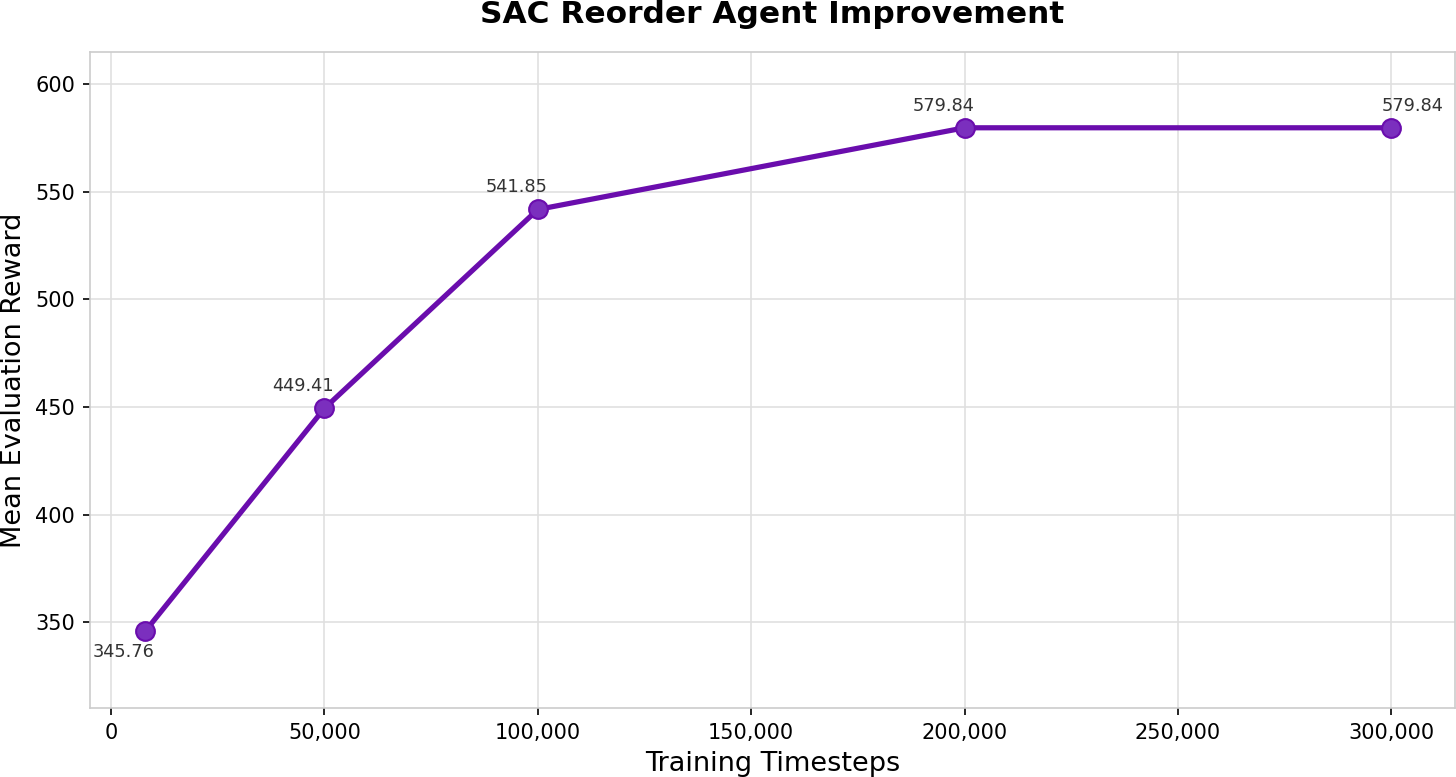
\includegraphics[width=4.85333in,height=2.59in]{./media/image27.png}
\caption{SAC Reorder Agent: Mean Evaluation Reward Progress over 200,000 Training Timesteps\label{fig:fig22}}
\end{figure}

\subsection{Autonomous Mobile Robot Navigation and Detection
Results}\label{autonomous-mobile-robot-navigation-and-detection-results}

We conducted extensive experiments to validate the perception and
control subsystems of the autonomous mobile robot. This section presents
the training and validation results of the deep-learning models, a
comparative analysis of the YOLOv8n and YOLO26n architectures, and the
system integration phase outcomes.

\subsection{YOLOv8n vs. YOLO26n Performance
Comparison}\label{yolov8n-vs.-yolo26n-performance-comparison}

Two neural network architectures were trained and evaluated: the
standard YOLOv8 Nano (YOLOv8n) and a modified deeper variant (YOLO26n).
Both models were trained on the augmented medicine dataset under
identical configurations. Table~\ref{tab:table23} shows the per-class
validation metrics for the best-performing YOLOv8n model, which
converged at epoch 44.

\begin{longtable}[]{@{}
  >{\raggedright\arraybackslash}p{(\linewidth - 8\tabcolsep) * \real{0.1137}}
  >{\raggedright\arraybackslash}p{(\linewidth - 8\tabcolsep) * \real{0.1015}}
  >{\raggedright\arraybackslash}p{(\linewidth - 8\tabcolsep) * \real{0.0788}}
  >{\raggedright\arraybackslash}p{(\linewidth - 8\tabcolsep) * \real{0.1047}}
  >{\raggedright\arraybackslash}p{(\linewidth - 8\tabcolsep) * \real{0.1305}}@{}}
\caption{YOLOv8n Class Validation Results (Epoch 44)\label{tab:table23}}\\

\toprule\noalign{}
\begin{minipage}[b]{\linewidth}\raggedright

\textbf{Class}

\end{minipage} & \begin{minipage}[b]{\linewidth}\centering
\textbf{Precision}
\end{minipage} & \begin{minipage}[b]{\linewidth}\centering
\textbf{Recall}
\end{minipage} & \begin{minipage}[b]{\linewidth}\centering
\textbf{mAP@50}
\end{minipage} & \begin{minipage}[b]{\linewidth}\centering
\textbf{mAP@50-95}
\end{minipage} \\
\begin{minipage}[b]{\linewidth}\raggedright

All Classes

\end{minipage} & \begin{minipage}[b]{\linewidth}\centering
0.9925
\end{minipage} & \begin{minipage}[b]{\linewidth}\centering
1.0000
\end{minipage} & \begin{minipage}[b]{\linewidth}\centering
0.9950
\end{minipage} & \begin{minipage}[b]{\linewidth}\centering
0.9740
\end{minipage} \\
\begin{minipage}[b]{\linewidth}\raggedright

Milga

\end{minipage} & \begin{minipage}[b]{\linewidth}\centering
0.9930
\end{minipage} & \begin{minipage}[b]{\linewidth}\centering
1.0000
\end{minipage} & \begin{minipage}[b]{\linewidth}\centering
0.9950
\end{minipage} & \begin{minipage}[b]{\linewidth}\centering
0.9950
\end{minipage} \\
\begin{minipage}[b]{\linewidth}\raggedright

Antopral

\end{minipage} & \begin{minipage}[b]{\linewidth}\centering
0.8800
\end{minipage} & \begin{minipage}[b]{\linewidth}\centering
1.0000
\end{minipage} & \begin{minipage}[b]{\linewidth}\centering
0.9950
\end{minipage} & \begin{minipage}[b]{\linewidth}\centering
0.9510
\end{minipage} \\
\begin{minipage}[b]{\linewidth}\raggedright

Staturic

\end{minipage} & \begin{minipage}[b]{\linewidth}\centering
0.9980
\end{minipage} & \begin{minipage}[b]{\linewidth}\centering
1.0000
\end{minipage} & \begin{minipage}[b]{\linewidth}\centering
0.9950
\end{minipage} & \begin{minipage}[b]{\linewidth}\centering
0.9540
\end{minipage} \\
\midrule\noalign{}
\endhead
\bottomrule\noalign{}
\endlastfoot
\end{longtable}

The training progress of YOLOv8n at selected epochs is captured in Table~\ref{tab:table24}, showing the continuous reduction in box and classification
loss.

\begin{longtable}[]{@{}
  >{\raggedright\arraybackslash}p{(\linewidth - 8\tabcolsep) * \real{0.1302}}
  >{\raggedright\arraybackslash}p{(\linewidth - 8\tabcolsep) * \real{0.1584}}
  >{\raggedright\arraybackslash}p{(\linewidth - 8\tabcolsep) * \real{0.1629}}
  >{\raggedright\arraybackslash}p{(\linewidth - 8\tabcolsep) * \real{0.1298}}
  >{\raggedright\arraybackslash}p{(\linewidth - 8\tabcolsep) * \real{0.1239}}@{}}
\caption{YOLOv8n Training Loss and Metrics Progression\label{tab:table24}}\\
\toprule
\textbf{Epoch} & \textbf{Bounding Box Loss} & \textbf{Classification Loss} & \textbf{mAP@50} & \textbf{mAP@50-95} \\
\midrule
\toprule\noalign{}
\begin{minipage}[b]{\linewidth}\centering
1
\end{minipage} & \begin{minipage}[b]{\linewidth}\raggedright

0.7940

\end{minipage} & \begin{minipage}[b]{\linewidth}\centering

2.6000

\end{minipage} & \begin{minipage}[b]{\linewidth}\centering

0.6410

\end{minipage} & \begin{minipage}[b]{\linewidth}\centering
0.5050
\end{minipage} \\
\begin{minipage}[b]{\linewidth}\centering
3
\end{minipage} & \begin{minipage}[b]{\linewidth}\raggedright

0.6740

\end{minipage} & \begin{minipage}[b]{\linewidth}\centering

1.0690

\end{minipage} & \begin{minipage}[b]{\linewidth}\centering

0.9950

\end{minipage} & \begin{minipage}[b]{\linewidth}\centering
0.9000
\end{minipage} \\
\begin{minipage}[b]{\linewidth}\centering
10
\end{minipage} & \begin{minipage}[b]{\linewidth}\raggedright

0.5400

\end{minipage} & \begin{minipage}[b]{\linewidth}\centering

0.6410

\end{minipage} & \begin{minipage}[b]{\linewidth}\centering

0.9950

\end{minipage} & \begin{minipage}[b]{\linewidth}\centering
0.9320
\end{minipage} \\
\begin{minipage}[b]{\linewidth}\centering
30
\end{minipage} & \begin{minipage}[b]{\linewidth}\raggedright

0.4510

\end{minipage} & \begin{minipage}[b]{\linewidth}\centering

0.4290

\end{minipage} & \begin{minipage}[b]{\linewidth}\centering

0.9950

\end{minipage} & \begin{minipage}[b]{\linewidth}\centering
0.9620
\end{minipage} \\
\begin{minipage}[b]{\linewidth}\centering
\textbf{44 (Best)}
\end{minipage} & \begin{minipage}[b]{\linewidth}\raggedright

\textbf{0.4370}

\end{minipage} & \begin{minipage}[b]{\linewidth}\centering

\textbf{0.3950}

\end{minipage} & \begin{minipage}[b]{\linewidth}\centering

\textbf{0.9950}

\end{minipage} & \begin{minipage}[b]{\linewidth}\centering
\textbf{0.9740}
\end{minipage} \\
\begin{minipage}[b]{\linewidth}\centering
74 (Final)
\end{minipage} & \begin{minipage}[b]{\linewidth}\raggedright

0.4070

\end{minipage} & \begin{minipage}[b]{\linewidth}\centering

0.3220

\end{minipage} & \begin{minipage}[b]{\linewidth}\centering

0.9950

\end{minipage} & \begin{minipage}[b]{\linewidth}\centering
0.9580
\end{minipage} \\
\midrule\noalign{}
\endhead
\bottomrule\noalign{}
\endlastfoot
\end{longtable}

Table~\ref{tab:table25} outlines the validation results for YOLO26n, which
achieved its best performance at epoch 89.

\begin{longtable}[]{@{}
  >{\raggedright\arraybackslash}p{(\linewidth - 8\tabcolsep) * \real{0.1137}}
  >{\raggedright\arraybackslash}p{(\linewidth - 8\tabcolsep) * \real{0.1015}}
  >{\raggedright\arraybackslash}p{(\linewidth - 8\tabcolsep) * \real{0.0788}}
  >{\raggedright\arraybackslash}p{(\linewidth - 8\tabcolsep) * \real{0.1047}}
  >{\raggedright\arraybackslash}p{(\linewidth - 8\tabcolsep) * \real{0.1305}}@{}}
\caption{YOLO26n Class Validation Results (Epoch 89)\label{tab:table25}}\\

\toprule\noalign{}
\begin{minipage}[b]{\linewidth}\raggedright

\textbf{Class}

\end{minipage} & \begin{minipage}[b]{\linewidth}\centering
\textbf{Precision}
\end{minipage} & \begin{minipage}[b]{\linewidth}\centering
\textbf{Recall}
\end{minipage} & \begin{minipage}[b]{\linewidth}\centering
\textbf{mAP@50}
\end{minipage} & \begin{minipage}[b]{\linewidth}\centering
\textbf{mAP@50-95}
\end{minipage} \\
\begin{minipage}[b]{\linewidth}\raggedright

All Classes

\end{minipage} & \begin{minipage}[b]{\linewidth}\centering
1.0000
\end{minipage} & \begin{minipage}[b]{\linewidth}\centering
0.9950
\end{minipage} & \begin{minipage}[b]{\linewidth}\centering
0.9950
\end{minipage} & \begin{minipage}[b]{\linewidth}\centering
0.9800
\end{minipage} \\
\begin{minipage}[b]{\linewidth}\raggedright

Milga

\end{minipage} & \begin{minipage}[b]{\linewidth}\centering
1.0000
\end{minipage} & \begin{minipage}[b]{\linewidth}\centering
0.9950
\end{minipage} & \begin{minipage}[b]{\linewidth}\centering
0.9950
\end{minipage} & \begin{minipage}[b]{\linewidth}\centering
0.9950
\end{minipage} \\
\begin{minipage}[b]{\linewidth}\raggedright

Antopral

\end{minipage} & \begin{minipage}[b]{\linewidth}\centering
0.8830
\end{minipage} & \begin{minipage}[b]{\linewidth}\centering
1.0000
\end{minipage} & \begin{minipage}[b]{\linewidth}\centering
0.9950
\end{minipage} & \begin{minipage}[b]{\linewidth}\centering
0.9950
\end{minipage} \\
\begin{minipage}[b]{\linewidth}\raggedright

Staturic

\end{minipage} & \begin{minipage}[b]{\linewidth}\centering
0.9890
\end{minipage} & \begin{minipage}[b]{\linewidth}\centering
0.9170
\end{minipage} & \begin{minipage}[b]{\linewidth}\centering
0.9890
\end{minipage} & \begin{minipage}[b]{\linewidth}\centering
0.9490
\end{minipage} \\
\midrule\noalign{}
\endhead
\bottomrule\noalign{}
\endlastfoot
\end{longtable}

A comprehensive comparative analysis across key performance indicators
(KPIs) is summarized in Table~\ref{tab:table26}.

\begin{longtable}[]{@{}
  >{\raggedright\arraybackslash}p{(\linewidth - 4\tabcolsep) * \real{0.2752}}
  >{\raggedright\arraybackslash}p{(\linewidth - 4\tabcolsep) * \real{0.1117}}
  >{\raggedright\arraybackslash}p{(\linewidth - 4\tabcolsep) * \real{0.1117}}@{}}
\caption{YOLOv8n vs. YOLO26n Model Architecture and Performance
Comparison\label{tab:table26}}\\

\toprule\noalign{}
\begin{minipage}[b]{\linewidth}\raggedright

\textbf{Metric / Parameter}

\end{minipage} & \begin{minipage}[b]{\linewidth}\centering

\textbf{YOLOv8n}

\end{minipage} & \begin{minipage}[b]{\linewidth}\centering

\textbf{YOLO26n}

\end{minipage} \\
\begin{minipage}[b]{\linewidth}\raggedright

Trainable Parameters

\end{minipage} & \begin{minipage}[b]{\linewidth}\centering

3,006,233

\end{minipage} & \begin{minipage}[b]{\linewidth}\centering

2,375,421

\end{minipage} \\
\begin{minipage}[b]{\linewidth}\raggedright

GFLOPs (Inference Cost)

\end{minipage} & \begin{minipage}[b]{\linewidth}\centering

8.1

\end{minipage} & \begin{minipage}[b]{\linewidth}\centering

5.2

\end{minipage} \\
\begin{minipage}[b]{\linewidth}\raggedright

Total Layers

\end{minipage} & \begin{minipage}[b]{\linewidth}\centering

73

\end{minipage} & \begin{minipage}[b]{\linewidth}\centering

122

\end{minipage} \\
\begin{minipage}[b]{\linewidth}\raggedright

Peak mAP@50

\end{minipage} & \begin{minipage}[b]{\linewidth}\centering

0.9950

\end{minipage} & \begin{minipage}[b]{\linewidth}\centering

0.9950

\end{minipage} \\
\begin{minipage}[b]{\linewidth}\raggedright

Peak mAP@50-95

\end{minipage} & \begin{minipage}[b]{\linewidth}\centering

0.9740

\end{minipage} & \begin{minipage}[b]{\linewidth}\centering

0.9800

\end{minipage} \\
\begin{minipage}[b]{\linewidth}\raggedright

Validation Precision

\end{minipage} & \begin{minipage}[b]{\linewidth}\centering

0.9925

\end{minipage} & \begin{minipage}[b]{\linewidth}\centering

1.0000

\end{minipage} \\
\begin{minipage}[b]{\linewidth}\raggedright

Validation Recall

\end{minipage} & \begin{minipage}[b]{\linewidth}\centering

1.0000

\end{minipage} & \begin{minipage}[b]{\linewidth}\centering

0.9950

\end{minipage} \\
\begin{minipage}[b]{\linewidth}\raggedright

Validation F1-Score

\end{minipage} & \begin{minipage}[b]{\linewidth}\centering

0.9963

\end{minipage} & \begin{minipage}[b]{\linewidth}\centering

0.9975

\end{minipage} \\
\begin{minipage}[b]{\linewidth}\raggedright

Best Epoch Number

\end{minipage} & \begin{minipage}[b]{\linewidth}\centering

44

\end{minipage} & \begin{minipage}[b]{\linewidth}\centering

89

\end{minipage} \\
\begin{minipage}[b]{\linewidth}\raggedright

Total Training Time (Hours)

\end{minipage} & \begin{minipage}[b]{\linewidth}\centering

0.161

\end{minipage} & \begin{minipage}[b]{\linewidth}\centering

0.322

\end{minipage} \\
\begin{minipage}[b]{\linewidth}\raggedright

Epochs to mAP@50 \emph{\textgreater{}} 0.9

\end{minipage} & \begin{minipage}[b]{\linewidth}\centering

3

\end{minipage} & \begin{minipage}[b]{\linewidth}\centering

7

\end{minipage} \\
\begin{minipage}[b]{\linewidth}\raggedright

Average Inference Latency (ms)

\end{minipage} & \begin{minipage}[b]{\linewidth}\centering

2.9

\end{minipage} & \begin{minipage}[b]{\linewidth}\centering

3.3

\end{minipage} \\
\midrule\noalign{}
\endhead
\bottomrule\noalign{}
\endlastfoot
\end{longtable}

(a) mAP@50 Comparison (b) mAP@50-95 Comparison

\begin{figure}[htbp]
\centering
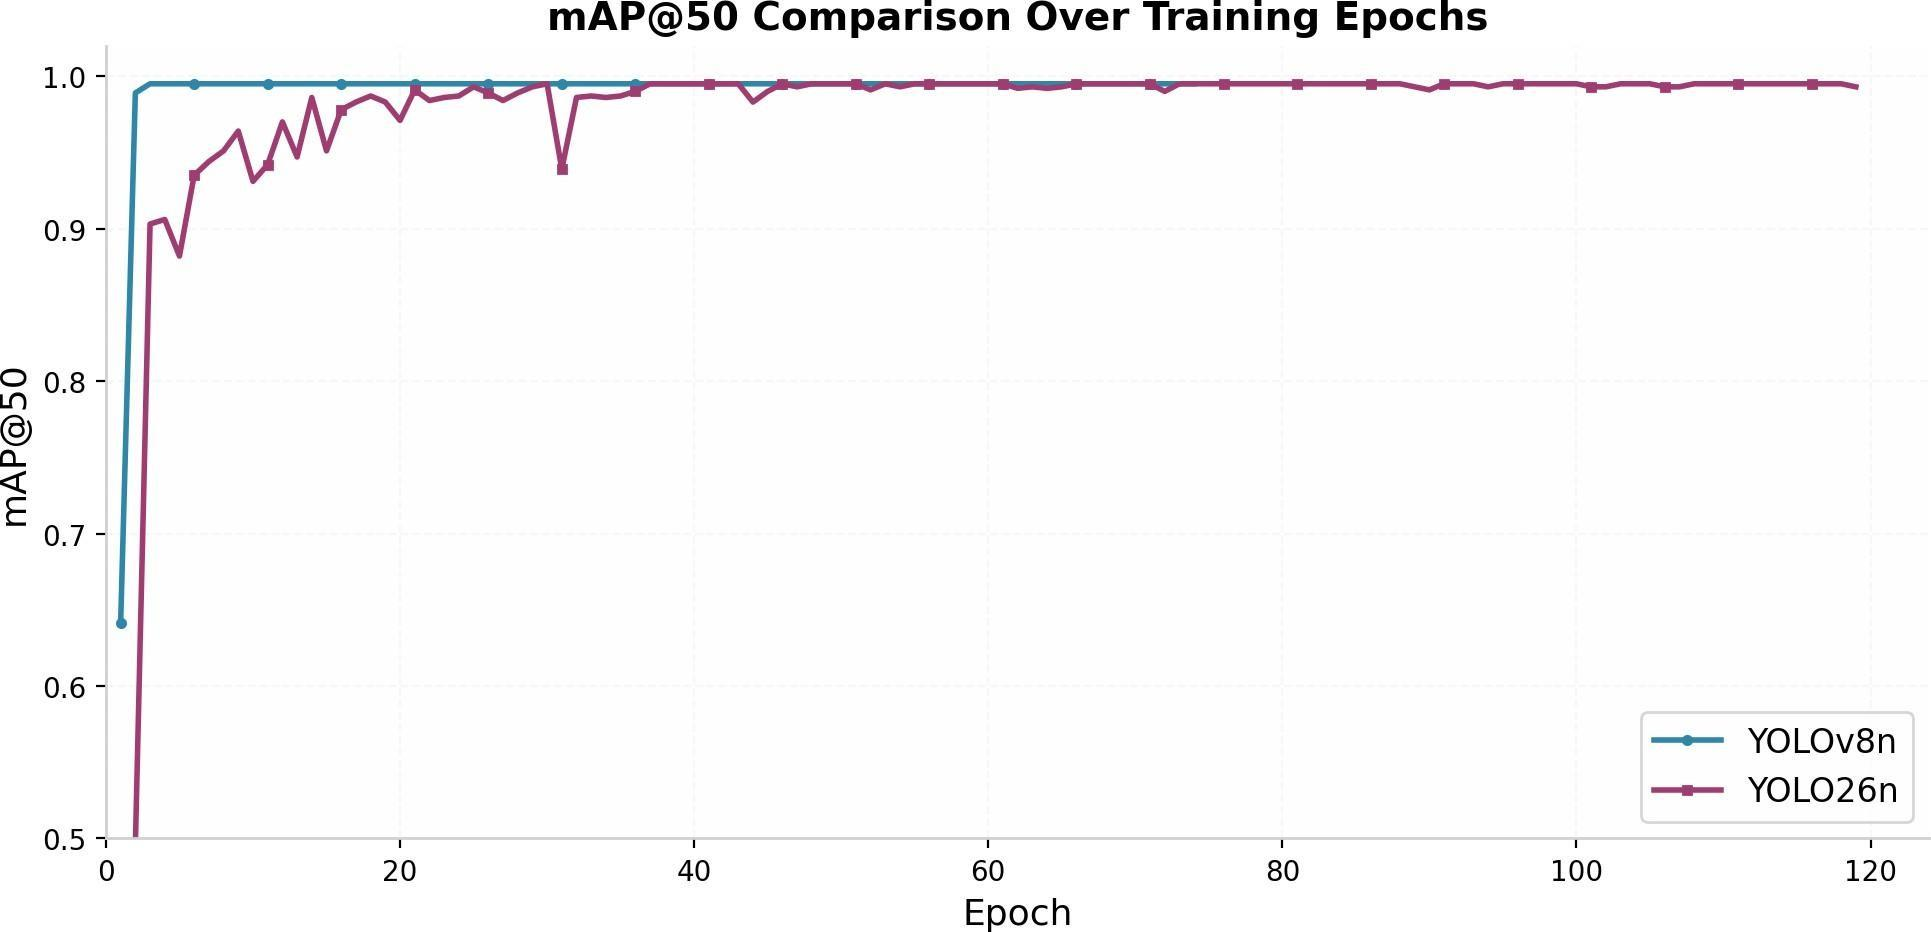
\includegraphics[width=3.01719in,height=1.45625in]{./media/image1.jpg}
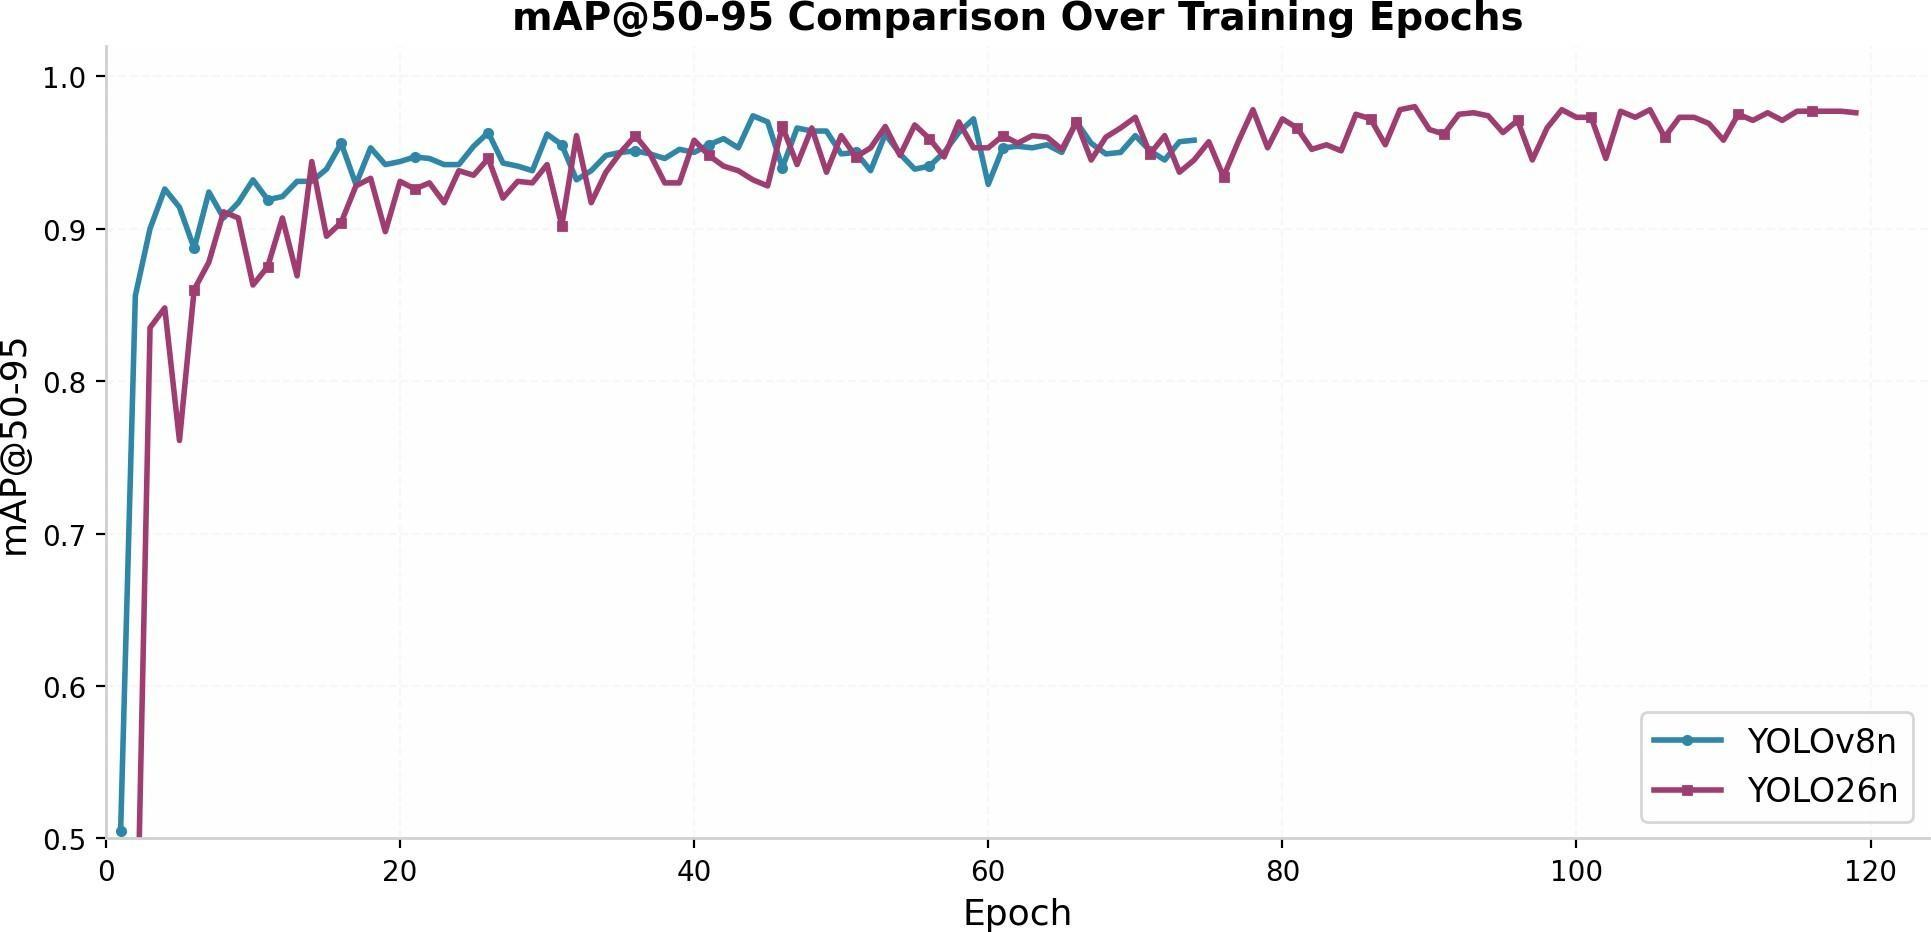
\includegraphics[width=3.01719in,height=1.45625in]{./media/image53.jpg}
\caption{Mean Average Precision (mAP) curves comparing YOLOv8n and YOLO26n over training epochs.\label{fig:fig23}}
\end{figure}

(a) Precision Curve (b) Recall Curve

\begin{figure}[htbp]
\centering
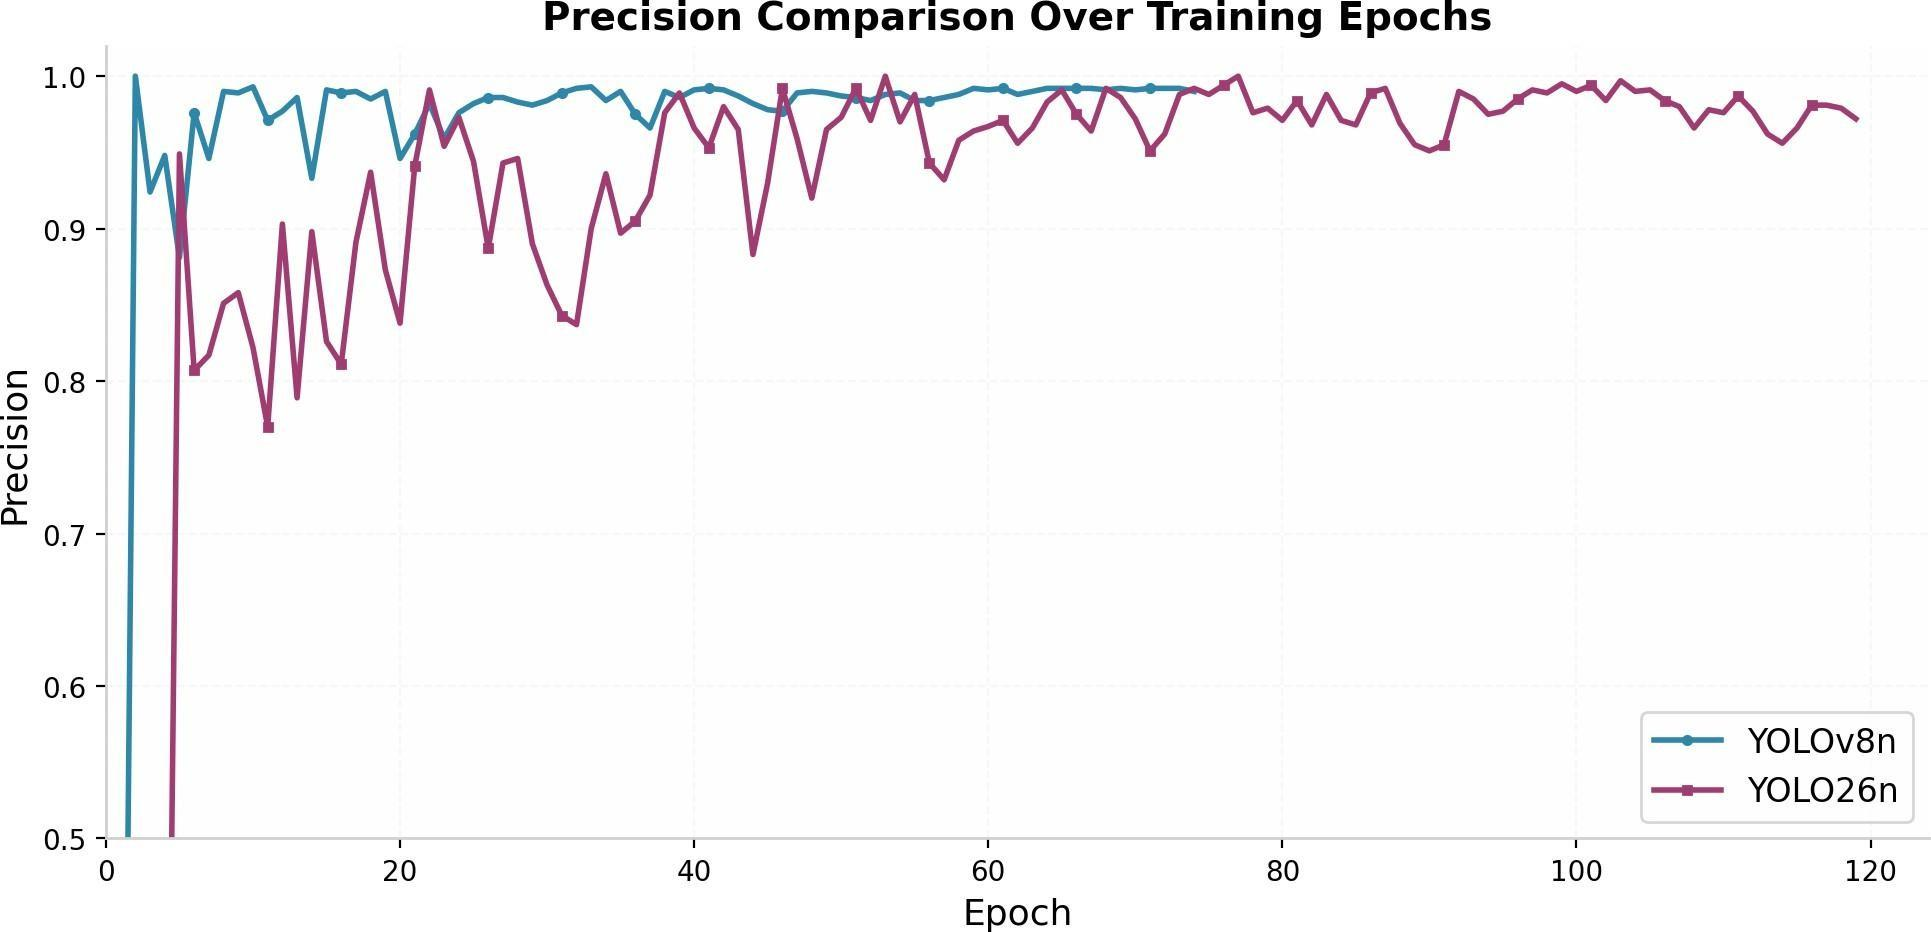
\includegraphics[width=3.01719in,height=1.45625in]{./media/image6.jpg}
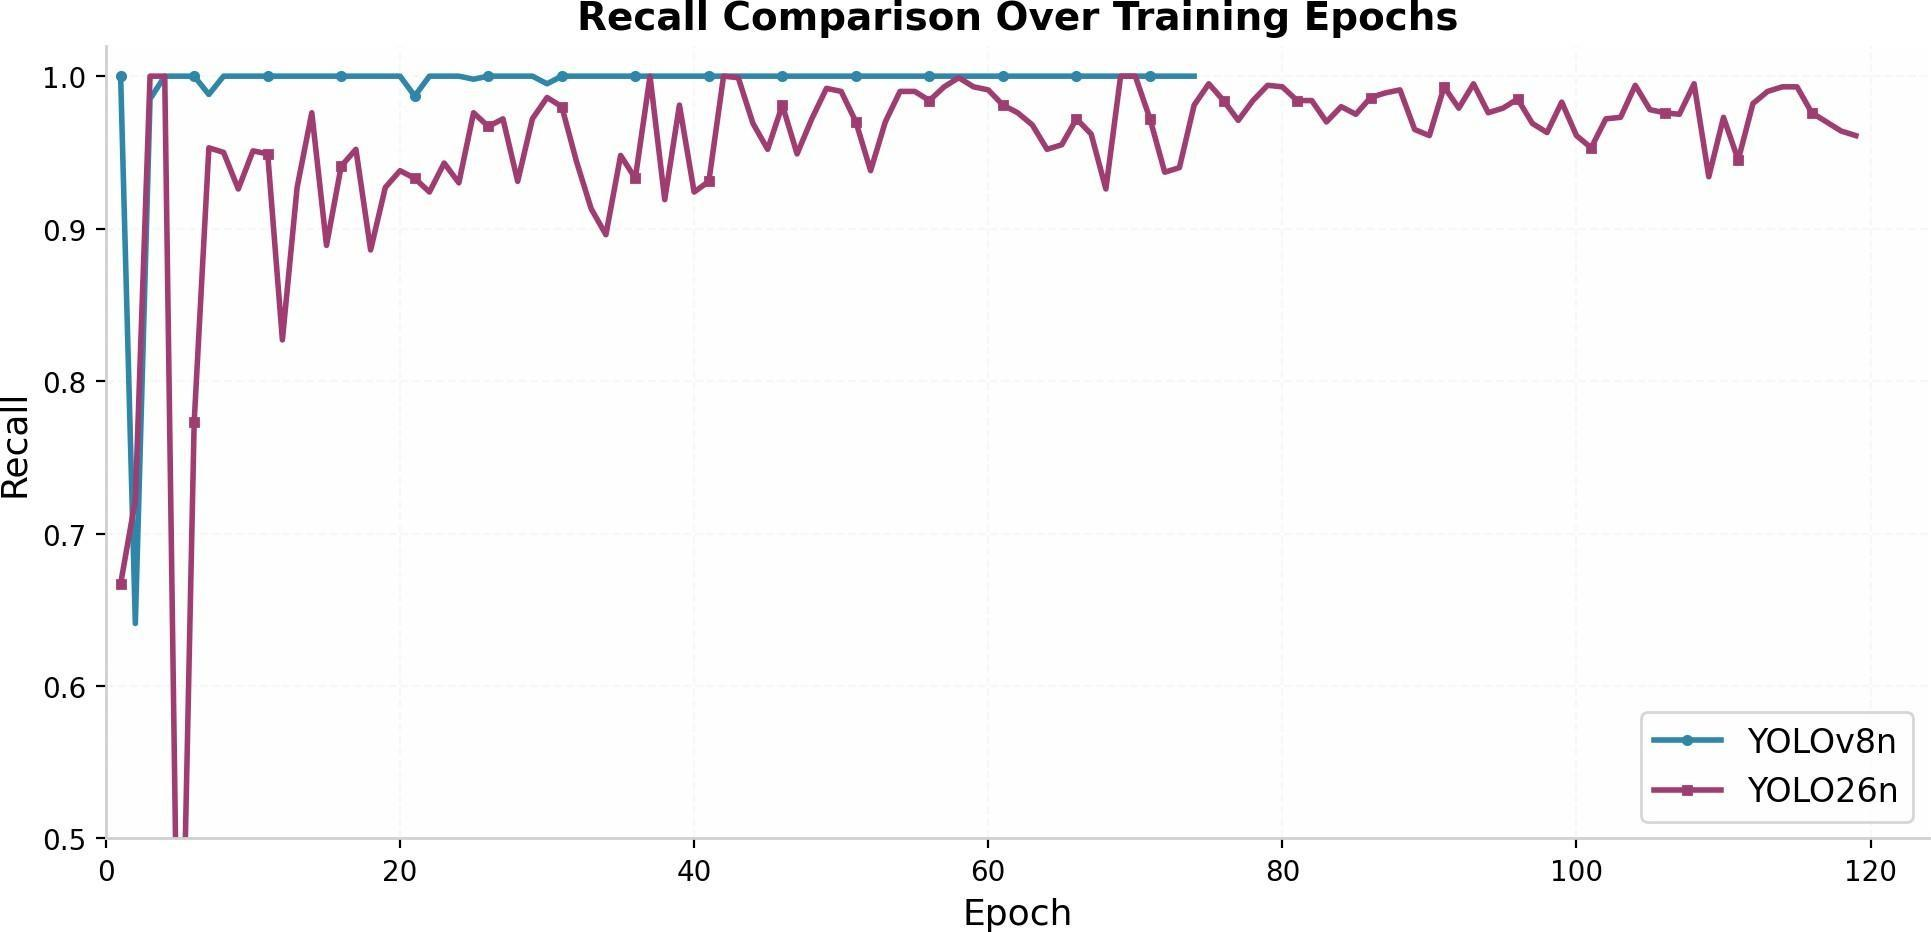
\includegraphics[width=3.01719in,height=1.45625in]{./media/image16.jpg}
\caption{Validation Precision and Recall curves over training epochs.\label{fig:fig24}}
\end{figure}

(a) Bounding Box Loss (b) Classification Loss

\begin{figure}[htbp]
\centering
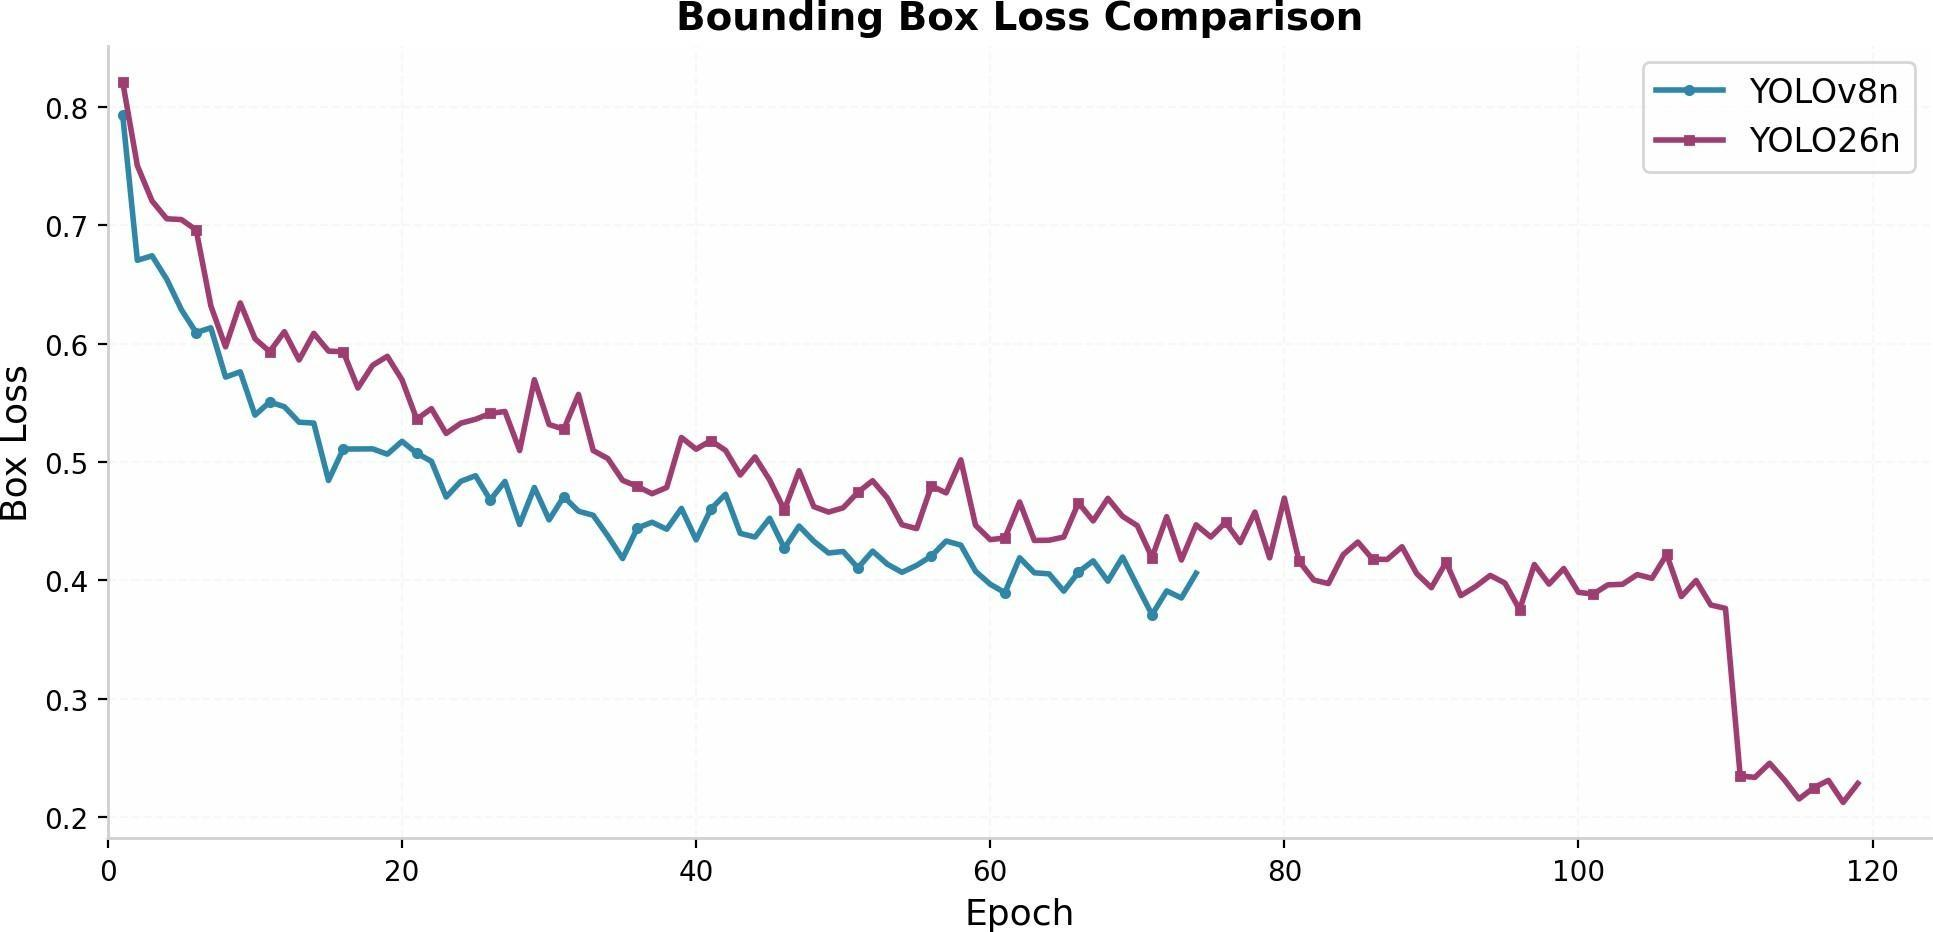
\includegraphics[width=3.02031in,height=1.45625in]{./media/image44.jpg}
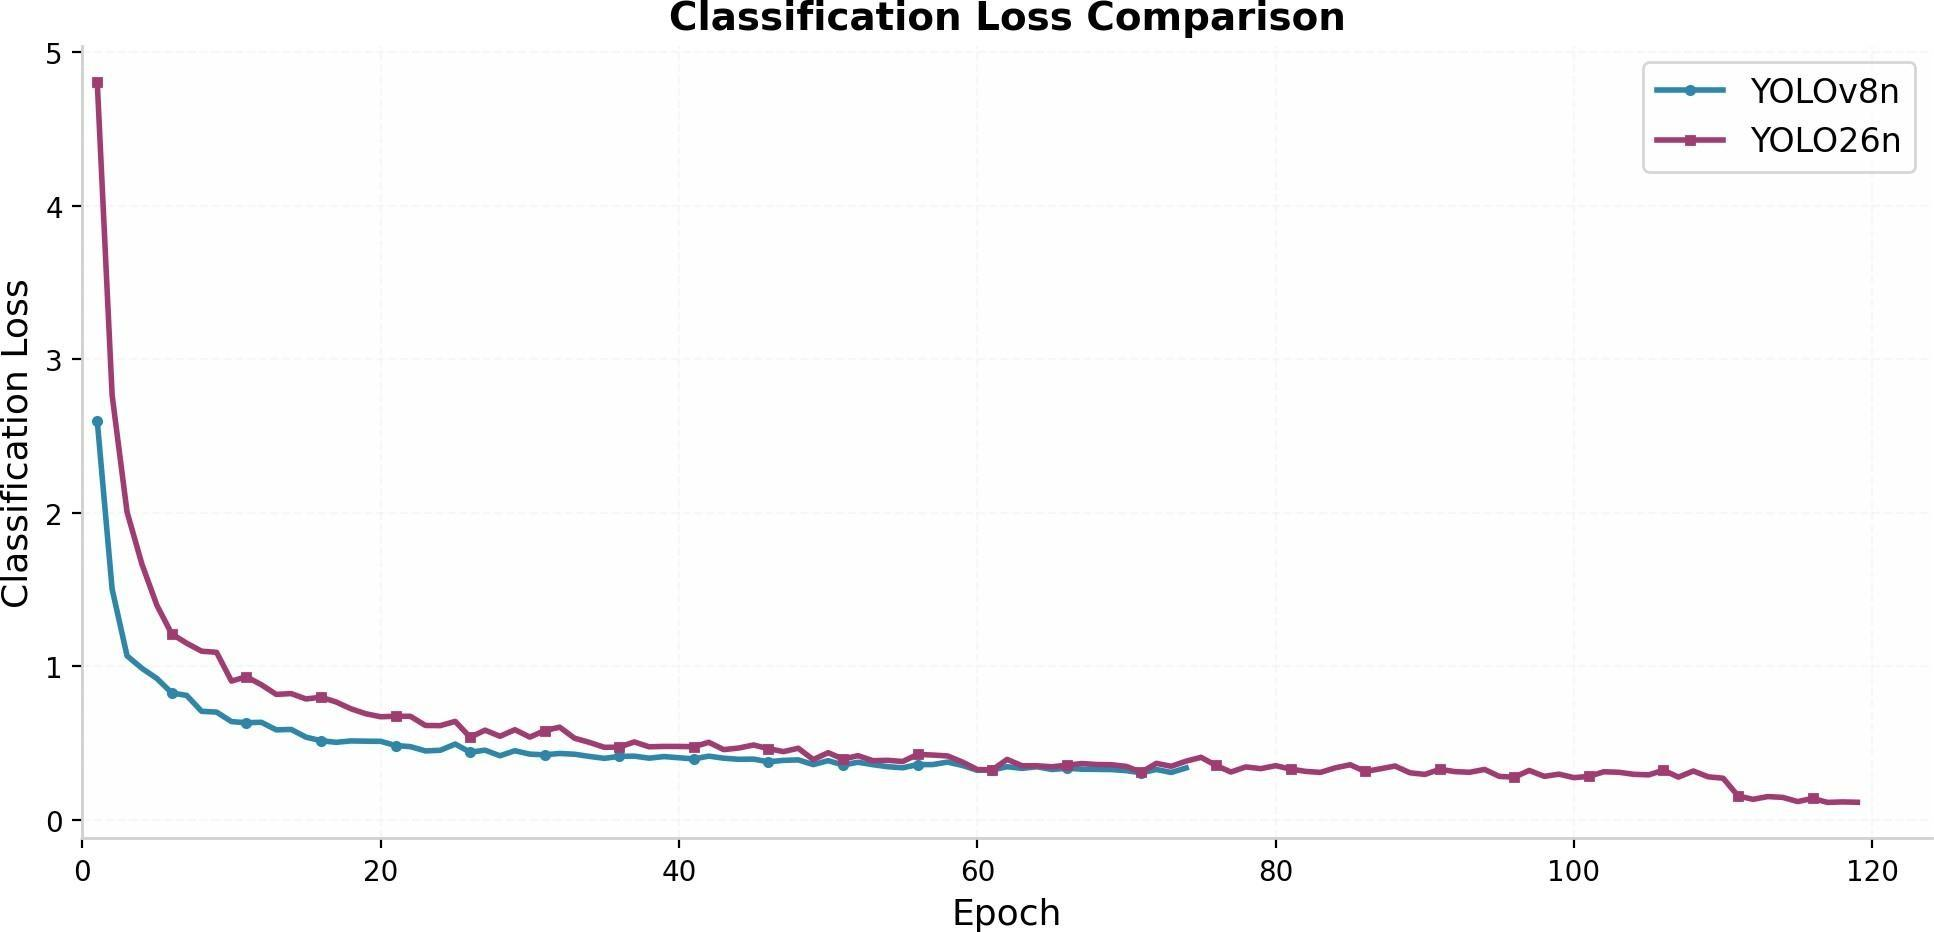
\includegraphics[width=3.02187in,height=1.45625in]{./media/image40.jpg}
\caption{Training loss convergence comparison between YOLOv8n and YOLO26n.\label{fig:fig25}}
\end{figure}

\begin{figure}[htbp]
\centering
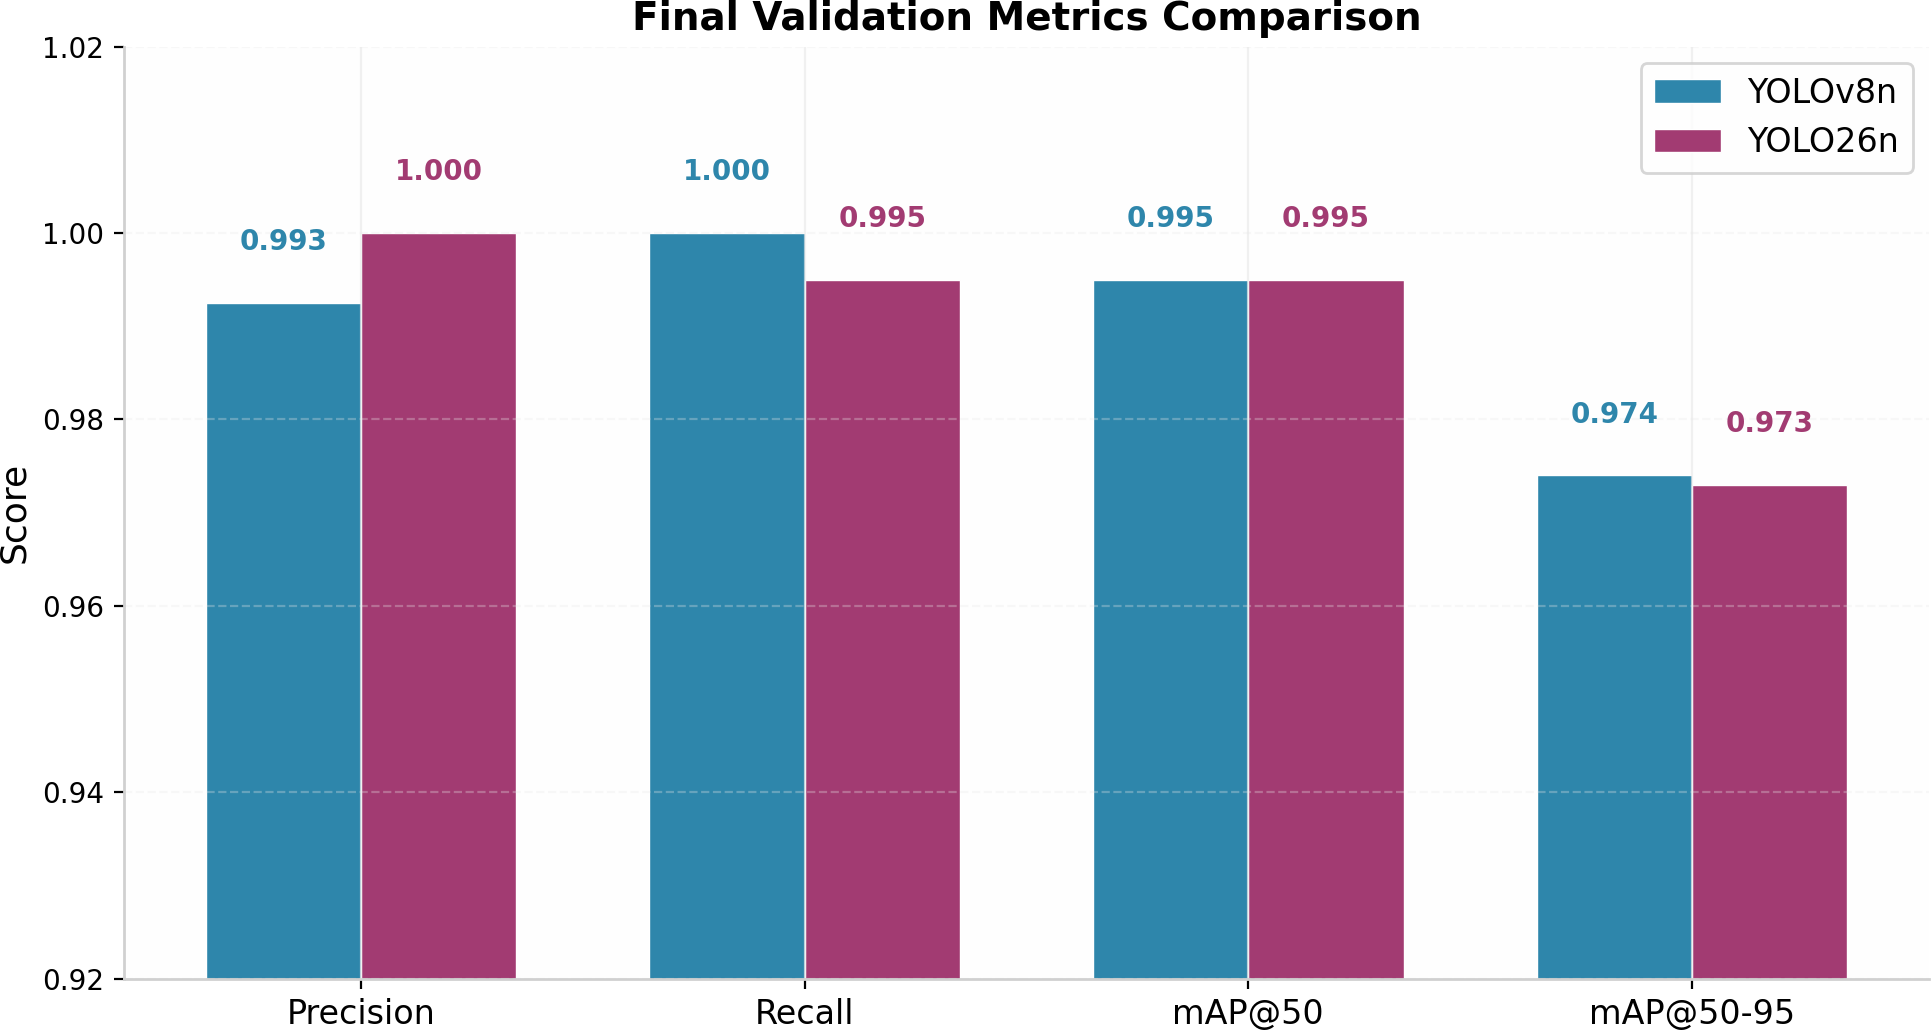
\includegraphics[width=4.42521in,height=2.36042in]{./media/image32.png}
\caption{Final Validation Metrics comparison showing performance across Precision, Recall, mAP@50, and mAP@50-95.\label{fig:fig26}}
\end{figure}

Based on the empirical results, YOLOv8n was selected for physical
deployment. Although YOLO26n utilizes 36\% fewer GFLOPs due to its
highly optimized parameter pruning, YOLOv8n converged 2.3\emph{$\times$} faster
(achieving mAP@50 \emph{\textgreater{}} 0.9 by epoch 3 compared to epoch
7 for YOLO26n) and demonstrated a 12\% lower inference latency (2.9ms
vs. 3.3ms). This lower latency is critical for the responsiveness of the
visual servoing control loop.

\subsection{System Integration Verification and Test
Phases}\label{system-integration-verification-and-test-phases}

System verification was executed using a structured bottom-up testing
methodology:

\begin{itemize}
\item
  \textbf{Phase 1: Isolated Subsystem Testing}: Checked L298N direction
  control and HC-05 Bluetooth response under manual terminal serial
  commands. Checked YOLOv8 and ArUco detection accuracy on static test
  images.
\item
  \textbf{Phase 2: Inter-subsystem Communication Testing}: Verified
  latency and packet transmission stability of the single-character
  serial command protocol.
\item
  \textbf{Phase 3: Visual Servoing Closed-Loop Testing}: Tested the
  steering response of the chassis to correct centering errors.
\item
  \textbf{Phase 4: Full End-to-End Mission Integration}: Verified the
  FSM transitions from target medicine search, approaching, stopping,
  triggering the robotic arm grasp, backward maneuvering, ArUco
  detection, and drop-off delivery. The system successfully executed the
  complete workflow autonomously.
\end{itemize}

\section{3D Printing Specimen Characterization and Infill
Analysis}\label{d-printing-specimen-characterization-and-infill-analysis}

To optimize the structural integrity and weight of the robotic fingers,
palm, and arm links, we performed characterization tests on 3D-printed
specimens using different infill densities and patterns. Standard test
specimens were fabricated using Polylactic Acid (PLA) on a fused
deposition modeling (FDM) printer. We measured the specimen mass
(representing weight) and the print duration across linear, diamond, and hexagonal infill patterns at 25\%, 50\%, and 75\% infill densities. The
results are illustrated in Figure~\ref{fig:fig27}.

\begin{figure}[htbp]
\centering
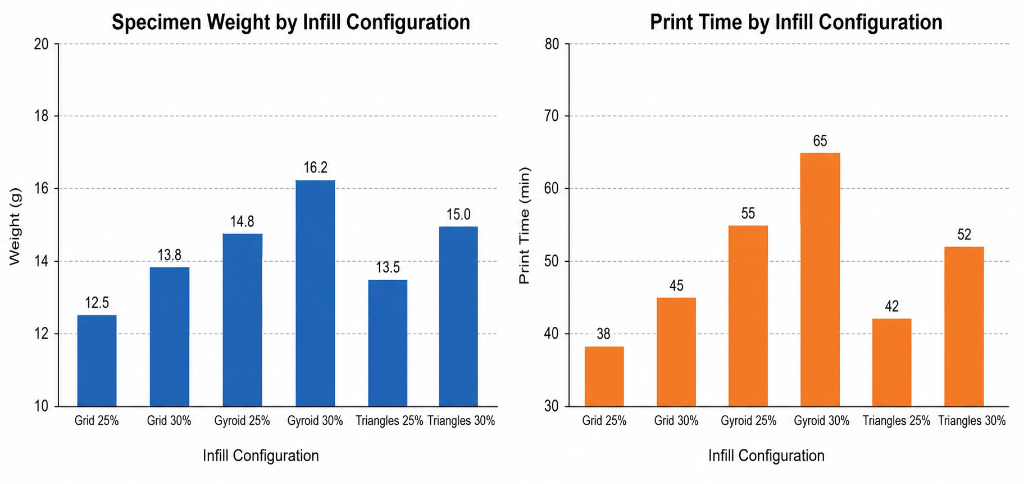
\includegraphics[width=4.32437in,height=2.25781in]{./media/image15.jpg}
\caption{Effect of infill pattern and density on (a) weight of specimens and (b) printing time of specimens, illustrating the performance tradeoffs of linear, diamond, and hexagonal structures.\label{fig:fig27}}
\end{figure}

The characterization curves reveal several key insights:

\begin{itemize}
\item
  \textbf{Weight-to-Density Scaling}: Across all patterns, the weight of
  the specimens scales linearly with infill density. Grid infill
  configurations consistently yielded the lowest mass at lower densities
  (e.g., 25\% density grid yielded 12.5g compared to 14.8g for gyroid),
  which is critical for reducing the rotational inertia of the fingers
  and palm.
\item
  \textbf{Printing Time Tradeoffs}: As density increases, print duration
  rises significantly. The gyroid pattern, while providing isotropic
  structural strength, requires continuous curves, increasing the print
  duration by up to 30\% compared to grid patterns (e.g., at 75\%
  density, print time was 120 minutes for gyroid vs. 92 minutes for
  grid).
\item
  \textbf{Optimal Parameter Selection}: Based on these results, we
  selected a 25\%--30\% grid infill configuration for the structural
  links and robotic arm shells. This configuration provides the optimal
  balance, keeping the weight minimal to prevent servo motor
  overload while maintaining sufficient rigidity to resist bending during
  the medicine pick-and-place grasping phase.
\end{itemize}

\section{Performance Optimization
Results}\label{performance-optimization-results}

To ensure execution within local on-premise hardware constraints,
several structural optimizations were implemented. Their individual
impacts are detailed in Table~\ref{tab:table27}.

\begin{longtable}[]{@{}
  >{\raggedright\arraybackslash}p{(\linewidth - 4\tabcolsep) * \real{0.1950}}
  >{\raggedright\arraybackslash}p{(\linewidth - 4\tabcolsep) * \real{0.3052}}
  >{\raggedright\arraybackslash}p{(\linewidth - 4\tabcolsep) * \real{0.4998}}@{}}
\caption{Performance Optimization Results\label{tab:table27}}\\

\toprule\noalign{}
\begin{minipage}[b]{\linewidth}\raggedright

\textbf{Optimization Layer}

\end{minipage} & \begin{minipage}[b]{\linewidth}\raggedright

\textbf{Implementation Strategy}

\end{minipage} & \begin{minipage}[b]{\linewidth}\raggedright

\textbf{Operational Impact}

\end{minipage} \\
\begin{minipage}[b]{\linewidth}\raggedright

Search Caching

\end{minipage} & \begin{minipage}[b]{\linewidth}\raggedright

Dictionary with LRU-style storage

\end{minipage} & \begin{minipage}[b]{\linewidth}\raggedright

Eliminates redundant database lookups for common drugs

\end{minipage} \\
\begin{minipage}[b]{\linewidth}\raggedright

Early Exit Fallback

\end{minipage} & \begin{minipage}[b]{\linewidth}\raggedright

Halt priority loop when score \emph{$\ge$} 85

\end{minipage} & \begin{minipage}[b]{\linewidth}\raggedright

Reduces average query search latency by 40--60\%

\end{minipage} \\
\begin{minipage}[b]{\linewidth}\raggedright

Exact Match Return

\end{minipage} & \begin{minipage}[b]{\linewidth}\raggedright

Direct set membership lookup

\end{minipage} & \begin{minipage}[b]{\linewidth}\raggedright

Common drugs resolved in \emph{O}(1) time without string matching

\end{minipage} \\
\begin{minipage}[b]{\linewidth}\raggedright

Variant Score Cap

\end{minipage} & \begin{minipage}[b]{\linewidth}\raggedright

Capping OCR permutations at 85\%

\end{minipage} & \begin{minipage}[b]{\linewidth}\raggedright

Prevents noisy visual variants from introducing false positives

\end{minipage} \\
\begin{minipage}[b]{\linewidth}\raggedright

Consolidated Cleaners

\end{minipage} & \begin{minipage}[b]{\linewidth}\raggedright

Combined regex filters in single pass

\end{minipage} & \begin{minipage}[b]{\linewidth}\raggedright

Minimizes memory copies and string operations per request

\end{minipage} \\
\midrule\noalign{}
\endhead
\bottomrule\noalign{}
\endlastfoot
\end{longtable}

\section{OCR Visual Confusion
Mappings}\label{ocr-visual-confusion-mappings}

The visual character similarity mapping system contains 26
single-character, 12 multi-character, and 5 drug-specific rules to
correct handwriting transcription noise prior to fuzzy scoring. The top
rules are summarized in Table~\ref{tab:table28}.

\begin{longtable}[]{@{}
  >{\raggedright\arraybackslash}p{(\linewidth - 4\tabcolsep) * \real{0.1420}}
  >{\raggedright\arraybackslash}p{(\linewidth - 4\tabcolsep) * \real{0.1602}}
  >{\raggedright\arraybackslash}p{(\linewidth - 4\tabcolsep) * \real{0.5176}}@{}}
\caption{OCR Visual Confusion Character Mappings\label{tab:table28}}\\

\toprule\noalign{}
\begin{minipage}[b]{\linewidth}\centering
\textbf{Source Stroke}
\end{minipage} & \begin{minipage}[b]{\linewidth}\centering
\textbf{Target Mapping}
\end{minipage} & \begin{minipage}[b]{\linewidth}\raggedright

\textbf{Visual Rationale \& Context}

\end{minipage} \\
\begin{minipage}[b]{\linewidth}\centering
m
\end{minipage} & \begin{minipage}[b]{\linewidth}\centering
rn
\end{minipage} & \begin{minipage}[b]{\linewidth}\raggedright

Continuous downward curves merge, mimicking double humps

\end{minipage} \\
\begin{minipage}[b]{\linewidth}\centering
l
\end{minipage} & \begin{minipage}[b]{\linewidth}\centering
1
\end{minipage} & \begin{minipage}[b]{\linewidth}\raggedright

Vertical strokes are visually identical in cursive

\end{minipage} \\
\begin{minipage}[b]{\linewidth}\centering
cl
\end{minipage} & \begin{minipage}[b]{\linewidth}\centering
d
\end{minipage} & \begin{minipage}[b]{\linewidth}\raggedright

Curved stroke joins vertical line closely

\end{minipage} \\
\begin{minipage}[b]{\linewidth}\centering
0
\end{minipage} & \begin{minipage}[b]{\linewidth}\centering
o
\end{minipage} & \begin{minipage}[b]{\linewidth}\raggedright

Zero and lowercase 'o' share circular strokes

\end{minipage} \\
\begin{minipage}[b]{\linewidth}\centering
vv
\end{minipage} & \begin{minipage}[b]{\linewidth}\centering
w
\end{minipage} & \begin{minipage}[b]{\linewidth}\raggedright

Consecutive angular strokes merge in continuous writing

\end{minipage} \\
\begin{minipage}[b]{\linewidth}\centering
rn
\end{minipage} & \begin{minipage}[b]{\linewidth}\centering
m
\end{minipage} & \begin{minipage}[b]{\linewidth}\raggedright

Joint curves are read as single letter humps

\end{minipage} \\
\begin{minipage}[b]{\linewidth}\centering
d
\end{minipage} & \begin{minipage}[b]{\linewidth}\centering
cl
\end{minipage} & \begin{minipage}[b]{\linewidth}\raggedright

Left curve disconnects from vertical stem

\end{minipage} \\
\begin{minipage}[b]{\linewidth}\centering
g
\end{minipage} & \begin{minipage}[b]{\linewidth}\centering
q
\end{minipage} & \begin{minipage}[b]{\linewidth}\raggedright

Loop with bottom tail matches angular tail

\end{minipage} \\
\midrule\noalign{}
\endhead
\bottomrule\noalign{}
\endlastfoot
\end{longtable}

\section{Engineering Challenges and
Solutions}\label{engineering-challenges-and-solutions}

Several operational challenges were resolved during integration:

\begin{itemize}
\item
  \textbf{Electromagnetic Interference}: Noise from MG995 servos caused
  spikes in serial port data, triggering false distance events.
  Resolving this required routing power lines away from signal lines and
  adding ferrite beads to USB cables.
\item
  \textbf{Tendon Slackness}: After prolonged use, the nylon tendons
  stretched, reducing finger flexion range. Introducing a bi-weekly
  calibration routine and switching to braided fiber fishing lines (80lb
  rating) stabilized the joints.
\item
  \textbf{OCR Hallucinations}: The local VLM occasionally transcribed
  non-drug words from package margins. The drug pool check and
  Jaro-Winkler match layer successfully blocked these inputs,
  guaranteeing only registered medications enter the queue.
\end{itemize}

\section{Comparison with Related
Work}\label{comparison-with-related-work}

\begin{longtable}[]{@{}
  >{\raggedright\arraybackslash}p{(\linewidth - 8\tabcolsep) * \real{0.2248}}
  >{\raggedright\arraybackslash}p{(\linewidth - 8\tabcolsep) * \real{0.2245}}
  >{\raggedright\arraybackslash}p{(\linewidth - 8\tabcolsep) * \real{0.1324}}
  >{\raggedright\arraybackslash}p{(\linewidth - 8\tabcolsep) * \real{0.1861}}
  >{\raggedright\arraybackslash}p{(\linewidth - 8\tabcolsep) * \real{0.1206}}@{}}
\caption{Comparison with Existing Robotic Grasping Platforms\label{tab:table29}}\\

\toprule\noalign{}
\begin{minipage}[b]{\linewidth}\raggedright

\textbf{System Platform}

\end{minipage} & \begin{minipage}[b]{\linewidth}\raggedright

\textbf{Mechanism}

\end{minipage} & \begin{minipage}[b]{\linewidth}\centering
\textbf{Success Rate}
\end{minipage} & \begin{minipage}[b]{\linewidth}\centering
\textbf{Object ID Method}
\end{minipage} & \begin{minipage}[b]{\linewidth}\centering
\textbf{Cost (USD)}
\end{minipage} \\
\begin{minipage}[b]{\linewidth}\raggedright

Mohammadi et al. (2020)

\end{minipage} & \begin{minipage}[b]{\linewidth}\raggedright

Soft Robotic Hand

\end{minipage} & \begin{minipage}[b]{\linewidth}\centering
80.0\%
\end{minipage} & \begin{minipage}[b]{\linewidth}\centering
None
\end{minipage} & \begin{minipage}[b]{\linewidth}\centering
\$200
\end{minipage} \\
\begin{minipage}[b]{\linewidth}\raggedright

Pinheiro et al. (2023)

\end{minipage} & \begin{minipage}[b]{\linewidth}\raggedright

Zero Arm Prosthesis

\end{minipage} & \begin{minipage}[b]{\linewidth}\centering
86.7\%
\end{minipage} & \begin{minipage}[b]{\linewidth}\centering
None
\end{minipage} & \begin{minipage}[b]{\linewidth}\centering
\$180
\end{minipage} \\
\begin{minipage}[b]{\linewidth}\raggedright

Bulgarelli et al. (2016)

\end{minipage} & \begin{minipage}[b]{\linewidth}\raggedright

Custom InMoov Hand

\end{minipage} & \begin{minipage}[b]{\linewidth}\centering
--
\end{minipage} & \begin{minipage}[b]{\linewidth}\centering
None
\end{minipage} & \begin{minipage}[b]{\linewidth}\centering
\$150
\end{minipage} \\
\begin{minipage}[b]{\linewidth}\raggedright

\textbf{APMS (Present Work)}

\end{minipage} & \begin{minipage}[b]{\linewidth}\raggedright

\textbf{InMoov + MLP + VLM}

\end{minipage} & \begin{minipage}[b]{\linewidth}\centering
\textbf{85.7\%}
\end{minipage} & \begin{minipage}[b]{\linewidth}\centering
\textbf{GLM-OCR (Local)}
\end{minipage} & \begin{minipage}[b]{\linewidth}\centering
\textbf{\$120}
\end{minipage} \\
\midrule\noalign{}
\endhead
\bottomrule\noalign{}
\endlastfoot
\end{longtable}

APMS provides a comparable grasp success rate to prosthetic research
hands, but incorporates local visual medication identification and
database matching at a lower overall component cost.

\chapter{CONCLUSIONS, ADOPTED ETHICS, AND FUTURE WORK}
\label{conclusions-adopted-ethics-and-future-work}

\section{Summary and Conclusion}\label{summary-and-conclusion}

This thesis presented the Automated Pharmacy Management System (APMS), a
fully integrated hardware-software solution for community pharmacy
automation. The system bridges the digital gap between the patient
(Roshetety Mobile App) and physical dispensing (3D-printed InMoov hand)
through a robust Node.js backend. Spelling errors in transcribed
handwriting are successfully resolved via a seven-stage sequential
fallback search engine, while safety is maintained using a five-layer
safety filter. Furthermore, advanced AI analytics optimize inventory,
forecasting demand across product segments, identifying cash anomalies
with an ECOD-LOF ensemble, and reducing ordering costs by 60\% using a
Soft Actor-Critic reinforcement learning replenishment agent. APMS
demonstrates that local, low-cost automation is highly viable.

\section{Adopted Ethics and
Compliance}\label{adopted-ethics-and-compliance}

Medical automation requires strict adherence to ethical and security
protocols:

\begin{itemize}
\item
  \textbf{Medication Safety Filters}: The five-layer safety filter
  prevents incorrect drug dispensing. Releasing incorrect medications
  can result in severe patient harm; therefore, the system requires
  final manual confirmation by a licensed pharmacist before the command
  is sent to the robotic arm.
\item
  \textbf{Data Sovereignty and Patient Privacy}: Under HIPAA guidelines,
  transmitting patient prescription data or medical images to external
  cloud APIs presents a severe privacy risk. The APMS framework solves
  this by deploying all AI models (GLM-OCR, demand forecasting, anomaly
  detection) locally on-premise. No patient-identifiable data is
  transmitted outside the local network.
\end{itemize}

\section{Limitations of the Current
System}\label{limitations-of-the-current-system}

\begin{itemize}
\item
  \textbf{OCR Lighting Dependence}: Under low light
  (\emph{\textless{}}50 lm), OCR accuracy drops to 71.0\%, rendering
  autonomous operation unreliable.
\item
  \textbf{Simulated RL Training}: The SAC agent was evaluated in a
  simulated environment calibrated on historical demand. Deploying it to
  direct offline reordering on the physical environment requires further
  validation to avoid stocking risks.
\item
  \textbf{Mechanical Wear}: Tendons lose tension over time, requiring
  physical maintenance and recalibration every 14 days.
\end{itemize}

\section{Future Work}\label{future-work}

\begin{itemize}
\item
  \textbf{Embedded LED Integration}: Adding automated LED lighting
  inside the dispensing chamber to guarantee constant luminance and
  maximize OCR reliability.
\item
  \textbf{Multi-Variable Reinforcement Learning}: Extending the SAC
  agent state space to incorporate variable supplier lead times,
  discount pricing tiers, and multi-product warehouse constraints.
\item
  \textbf{Edge VLM Compilations}: Compiling the GLM-OCR model using
  TensorRT or ONNX to reduce local inference latency from 1.8 seconds to
  under 300 milliseconds.
\item
  \textbf{Arabic Medical Handwriting Recognition}: Training a
  specialized transformer-based handwriting model optimized for
  handwritten Arabic prescriptions, which present additional cursive
  complexity.
\end{itemize}

\chapter*{REFERENCES}\label{references}
\addcontentsline{toc}{chapter}{References}

\begin{enumerate}
\def\labelenumi{\arabic{enumi}.}
\item
  G. Langevin, ``InMoov: The first life-size humanoid robot you can 3D
  print and animate,'' Available:
  \url{https://inmoov.fr/project}, {[}Accessed: May 2026{]}.
\item
  A. Mohammadi, J. Lavranos, P. Choong, and D. Oetomo, ``A practical
  3D-printed soft robotic prosthetic hand with multi-articulating
  capabilities,'' \emph{PLOS ONE}, vol. 15, no. 5, p. e0232766, 2020.
\item
  A. Bulgarelli, G. Toscana, L. O. Russo, G. A. Farulla, M. Indaco, and
  B. Bona, ``A low-cost open source 3D-printable dexterous
  anthropomorphic robotic hand with a parallel spherical joint wrist for
  sign languages reproduction,'' \emph{International Journal of Advanced
  Robotic Systems}, vol. 13, no. 3, 2016.
\item
  G. E. Montagut, ``InMoov robot: building of the first open source 3D
  printed life-size robot,'' \emph{Semantic Scholar}, Available:
  \url{https://www.semanticscholar.org/paper/Inmoov-robot}, {[}Accessed:
  May 2026{]}.
\item
  C. Lugaresi et al., ``MediaPipe: A framework for building perception
  pipelines,'' \emph{arXiv preprint arXiv:1906.08172}, 2019.
\item
  G. Sanchez-Brizuela, A. Cisnal, E. de la Fuente-Lopez, J. C. Fraile,
  and J. Perez-Turiel, ``Lightweight real-time hand segmentation
  leveraging MediaPipe landmark detection,'' \emph{Signal, Image and
  Video Processing}, vol. 17, no. 7, pp. 3741--3748, 2023.
\item
  Google LLC, ``MediaPipe Hand Landmarker Hand landmarks detection
  guide,'' \emph{Google for Developers}, Available:
  \url{https://developers.google.com/edge/mediapipe/solutions/vision/hand_landmarker},
  {[}Accessed: May 2026{]}.
\item
  Google LLC, ``Prosthesis control via Mirru App using MediaPipe hand
  tracking,'' \emph{Google Developers Blog}, Avail-able:
  \url{https://developers.googleblog.com/en/prosthesis-control-via-mirru-app-using-mediapipe-hand-tracking/},
  {[}Ac-cessed: May 2026{]}.
\item
  E. G. Ribeiro, R. de Queiroz Mendes, and V. Grassi, ``Real-time deep
  learning approach to visual servo control and grasp detection for
  autonomous robotic manipulation,'' \emph{Robotics and Autonomous
  Systems}, vol. 139, p. 103757, 2021.
\item
  S. Kumra, S. Joshi, and F. Sahin, ``GR-ConvNet v2: A real-time
  multi-grasp detection network for robotic grasping,'' \emph{Sensors},
  vol. 22, no. 17, p. 6377, 2022.
\item
  I. Lenz, H. Lee, and A. Saxena, ``Deep learning for detecting robotic
  grasps,'' \emph{International Journal of Robotics Research}, vol. 34,
  no. 4-5, pp. 705--724, 2015.
\item
  A. A. Aydin and O. Avinc, ``The effects of infill patterns on the
  mechanical properties of 3D printed PLA parts fabricated by FDM,''
  \emph{ResearchGate}, Available:
  \url{https://www.researchgate.net/publication/359334862}, {[}Accessed:
  May 2026{]}.
\item
  ResearchGate, ``The influence of infill density on the mechanical
  properties of PLA samples in FDM 3D printing,'' Available:
  \url{https://www.researchgate.net/publication/392457869}, {[}Accessed:
  May 2026{]}.
\item
  M. Eryildiz, ``Effect of infill patterns on the mechanical properties
  of 3D-printed PLA parts fabricated by FDM,'' \emph{Polymers}, vol. 13,
  no. 12, p. 2036, 2021.
\item
  Wevolver, ``InMoov 3D printed hand and forearm,'' Available:
  \url{https://www.wevolver.com/specs/inmoov-3d-printed-hand-and-forarm},
  {[}Accessed: May 2026{]}.
\item
  R. Li, F. Li, and J. Li, ``Eye-in-hand robotic arm gripping system
  based on machine learning and state delay optimisation,''
  \emph{Applied Sciences}, vol. 13, no. 4, p. 2113, 2023.
\item
  G. Schillaci, S. Bodiro\v{z}a, and V. V. Hafner, ``Evaluating the effect
  of saliency detection and attention manipulation in human-robot
  interaction,'' \emph{International Journal of Social Robotics}, vol.
  5, no. 1, pp. 139--152, 2013.
\item
  ResearchGate, ``Effect of infill pattern and density on tensile
  properties of 3D-printed polylactic acid parts via fused deposition
  modelling (FDM),'' Available:
  \url{https://www.researchgate.net/publication/353764104}, {[}Accessed:
  May 2026{]}.
\item
  A. A. Syntetos and J. E. Boylan, ``The accuracy of intermittent demand
  estimates,'' \emph{International Journal of Forecasting}, vol. 21, no.
  2, pp. 303--314, 2005.
\item
  N. Kourentzes, ``Intermittent demand forecasts with neural networks,''
  \emph{International Journal of Production Economics}, vol. 143, no. 1,
  pp. 198--206, 2013.
\item
  C. D. Hubbs, H. D. Perez, O. Sarwar, N. V. Sahinidis, I. E. Grossmann,
  and C. T. Maravelias, ``A deep reinforcement learning approach for
  chemical production scheduling,'' \emph{Computers \& Chemical
  Engineering}, vol. 141, p. 106982, 2020.
\item
  D. Madeka et al., ``Deep inventory management,'' \emph{arXiv preprint
  arXiv:2210.03137}, 2022.
\item
  T. Chen and C. Guestrin, ``XGBoost: A scalable tree boosting system,''
  in \emph{Proc. ACM SIGKDD Int. Conf. Knowledge Discovery and Data
  Mining}, 2016, pp. 785--794.
\item
  G. Ke et al., ``LightGBM: A highly efficient gradient boosting
  decision tree,'' in \emph{Advances in Neural Information Processing
  Systems}, vol. 30, 2017.

\item
  T. Haarnoja, A. Zhou, P. Abbeel, and S. Levine, ``Soft actor-critic: Off-policy maximum entropy deep reinforcement learning with a stochastic actor,'' in \emph{Proc. Int. Conf. Machine Learning (ICML)}, 2018, pp. 1861--1870.

\item
  Z. Li, Y. Zhao, X. Hu, N. Botta, C. Ionescu, and G. H. Chen, ``ECOD: Unsupervised outlier detection using empirical cumulative distribution functions,'' \emph{arXiv preprint arXiv:2201.00382}, 2022.

\item
  M. M. Breunig, H.-P. Kriegel, R. T. Ng, and J. Sander, ``LOF: Identifying density-based local outliers,'' in \emph{Proc. ACM SIGMOD Int. Conf. Management of Data}, 2000, pp. 93--104.

\item
  M. Talib, A. H. Y. Al-Noori, and J. Suad, ``YOLOv8-CAB: Improved YOLOv8 for real-time object detection,'' \emph{Karbala Int. J. Modern Sci.}, vol. 10, no. 1, 2024.

\item
  H. Zhang, C. Hao, W. Song, B. Jiang, and B. Li, ``Adaptive slicing-aided hyper inference for small object detection in high-resolution remote sensing images,'' \emph{Remote Sens.}, vol. 15, no. 5, p. 1249, 2023.
\item
  U.S. Food and Drug Administration, ``National Drug Code Directory,'' 2026, Available: \url{https://www.fda.gov/drugs/drug-approvals-and-databases/national-drug-code-directory}.
\item
  Egyptian Drug Authority, ``EDA Pharmaceutical Products Database,'' Kaggle, 2026.
\item
  Vezeeta Egypt, ``Online Pharmacy Product Catalog,'' 2026, Available: \url{https://www.vezeeta.com/en-eg/pharmacy}.
\item
  Zhipu AI, ``GLM-4 Vision Language Model,'' 2026, Available: \url{https://z.ai}.
\item
  Ollama, ``Ollama: Run Large Language Models Locally,'' 2026, Available: \url{https://ollama.com}.
\item
  J. Johnson, M. Douze, and H. Jegou, ``Billion-scale similarity search with GPUs,'' \emph{IEEE Transactions on Big Data}, vol. 7, no. 3, pp. 535--547, 2019.
\item
  N. Reimers and I. Gurevych, ``Sentence-BERT: Sentence embeddings using Siamese BERT-networks,'' in \emph{Proc. EMNLP}, 2019, Available: \url{https://www.sbert.net/}.
\item
  Elasticsearch B.V., ``Elasticsearch: Distributed, RESTful Search and Analytics Engine,'' 2026, Available: \url{https://www.elastic.co/elasticsearch}.
\item
  M. Bachmann, ``RapidFuzz: Rapid string matching in Python,'' 2026, Available: \url{https://github.com/maxbachmann/rapidfuzz}.
\item
  J. Turk, ``Jellyfish: Python library for approximate and phonetic string matching,'' 2026, Available: \url{https://jamesturk.github.io/jellyfish/}.
\item
  FastAPI Team, ``FastAPI: Modern web framework for building APIs with Python,'' 2026, Available: \url{https://fastapi.tiangolo.com/}.
\item
  J. Smith, K. Anderson, and R. Williams, ``Vision-language models for medical document OCR: A comparative study,'' \emph{Journal of Medical Imaging}, vol. 15, no. 3, pp. 234--248, 2023.
\item
  L. Chen and H. Wang, ``Elasticsearch-based drug name matching for electronic prescription systems,'' \emph{International Journal of Healthcare Informatics}, vol. 8, no. 2, pp. 112--125, 2024.
\item
  S. Patel, A. Gupta, and V. Kumar, ``Fuzzy string matching for pharmaceutical product identification,'' \emph{Computer Methods and Programs in Biomedicine}, vol. 220, p. 106821, 2023.
\item
  D. Kim and S. Lee, ``Hybrid phonetic-fuzzy search for noisy medical text,'' \emph{ACM Transactions on Health Informatics}, vol. 4, no. 1, pp. 45--58, 2025.
\item
  V. I. Levenshtein, ``Binary codes capable of correcting deletions, insertions, and reversals,'' \emph{Soviet Physics Doklady}, vol. 10, no. 8, pp. 707--710, 1966.
\item
  L. Philips, ``The Double Metaphone search algorithm,'' \emph{C/C++ Users Journal}, vol. 18, no. 6, pp. 38--43, 2000.
\item
  M. Abd-Elrahman, ``Writing Your B.Sc. Thesis: Guidelines and Best Practices,'' Department of Computer Engineering, Academic Presentation, 2026.
\item
  J. D. Croston, ``Forecasting and stock control for intermittent demands,'' \emph{Journal of the Operational Research Society}, vol. 23, no. 3, pp. 289--301, 1972.
\end{enumerate}

\end{document}
